%%**************************************************************************************************
%%
%% File Name : PhysNote_CM.tex
%% 説明      : 物理学の導入をかねた,古典力学(ニュートン力学と解析力学)を学習する.
%%
%%**************************************************************************************************
%===================================================================================================
%  Chapter : 物理学への導入
%  説明    : 物理学の基本的な考え方(定義,法則等)について説明する.
%===================================================================================================
\chapter{物理学への導入}
%   %-----------------------------------------------------------------------------------------------
%   %  Input
%   %    File Name : PhysNote_CM_PhysIntro.tex
%   %    説明      : 物理学の基本的な考え方(定義,法則等)について説明する.
%   %-----------------------------------------------------------------------------------------------
        e;;%===================================================================================================
%  Chapter : 物理学への導入
%  説明    : 物理学の基本的な考え方(定義,法則等)について説明する.
%===================================================================================================
%   %==========================================================================
%   %  Section
%   %==========================================================================
    \section{物理学を勉強する理由}
        \begin{mycomment}
            これから物理学を勉強していく.だけどその前に,物理学を勉強する理由について述べておきたい.
            このノートでの理由は,簡単に言ってしまえば,"知りたい" とういう衝動である.
            単純な興味から物理学の教科書やWebサイトなどを読んで,それを理解することで満足感を得ることだ.
            以下,もう少し一般的な視点で記述しておく.
        \end{mycomment}

%       %======================================================================
%       %  SubSection
%       %======================================================================
        \subsection{科学を勉強する}
        \subsubsection{科学とは何か}
            物理学は科学の基礎となる分野である.
            全ての他の科学は,究極的には,物理学によって説明できるはずである
                \footnote{
                    根拠はない.大袈裟かもしれない.この見解は間違っているかもしれない.
                    でも,すべての科学理論が物理学に帰着できると信じている.
                }.
            物理学のノートを作成するにあたり,最初に,科学的活動に
            ついてのイメージを記述しておくべきだろう.

            科学に対するイメージとして有名なのは,次の2つであろう.
                \begin{description}
                    \item[ (1)] 科学とは,世の中の複雑な現象を解析し,理解するための活動である.
                    \item[ (2)] 科学とは,世の中の複雑な現象に対して,最も単純な説明を与える活動である.
                \end{description}
            (1)のイメージは,「真の自然法則を追い求めることが科学である」と
            いう主張である.これに対し,(2)のイメージは,「科学は自然現象の良い説明の探求」
            である.要するに,(1)の考え方では,科学によって真の自然の姿を見出すことが可能である
            と信じるのだが,翻って(2)の考え方によると
                \footnote{
                    翻る(ひるがえる):態度・説などが、急に変わって反対になる
                },
            科学では自然の真の姿を見出すことではなく
                \footnote{
                    (2)の考え方では,科学は真の自然の姿を見出すことはできないという
                    立場である.
                },
            それに限りなく近づくことである,ということである.
            (1)の考え方をとると,自然の姿そのものの探求となるが,(2)の考え方では
            自然現象の"説明"の探求ということになる.この2つの考え方はどちらも間違っては
            いないように思える.科学を熱く語る場合には(1)の立場になりがちだが,それを
            冷静に反省している時には(2)の立場になることだろう.

            科学とは何かとか,どういった活動かを考える学問分野に,\textbf{科学哲学} がある.
            科学哲学は人間が行う科学的な活動について研究する分野で,法則の信頼性であるとか,
            科学的推論の妥当性だとかを見直す必要があることを示してくれる.

            実は「科学とは何か」という疑問は奥が深い.実際,未だに万人が賛成するような
            結論がない.ここでは,科学とは何かという問題は思ったよりも難しいものである
            ことを認識してもらって,学習を先に進めよう.学習をすすめる過程で,科学とは
            どういったことかを体験できるであろう
                \footnote{
                    ただし,言葉で説明するのではなく,実際に物理学の学習を通して,
                    その感覚を覚えるということである.
                }.

             とりあえず,やってみること.そして,それをやり続けること.そうする中で,一度立ち止まり,
             今までやってきたことを反省してみる.そうすることで,科学とは何かを悟るしかない.
             もともと,科学という活動基準があったのではない.ある活動を後から反省すると,
             その中に,特別な思想に従った活動であることを見出し,その活動に科学という
             名前を与えたのだ.これはきっと,科学だけではなく,他の学問に対しても,
             同じことが言えるだろう.

        \subsubsection{科学活動の原動力は好奇心だ}
            なぜ,自然現象を理解したり,それを説明しようとするのか.
            その理由は,別に大した理由ではなく,
            単に,"知りたいから" という知的好奇心によるものであろう.
            工学的な仕事をしている私にとっては,「世の中の原理を解明して,それを利用することで,
            より暮らしが豊かになるような装置を作ることができる」ときれいごとを言うことが
            できるかもしれないが,これは建前であり本心ではない.

            日常生活で不思議に感じる現象やモノについて,その性質や特徴を調べて,整理する.
            もしその複雑な現象を人間が理解し,更に制御できるようになれば,
            その現象を利用した,よりよい世界を構築できる.本当にそうなのだろうか.
            科学的活動を行う動機や理由は人それぞれで,絶対的な答えはないかもしれない.
            それでも,次のことだけは言えると思う.

            「世の中には不思議な現象がたくさんある.
            人間は不思議なことをそのまま放っておくことができない.
            自分が納得し不思議がなくなるまで追求し続けなければ,気が済まない」

        \subsubsection{科学的活動の手順}
            具体的に科学的活動をするには,どうすればよいのだろうか.
            いや,そもそも,私に科学的活動が行えるだろうか.
            結論から言うと,残念ながら,私のような人間には科学的活動はできない.
            理由は簡単で,私が理解力に乏しく,発想力もないからだ.科学的活動に
            必要なのは,認識力や観察力や発想力であり,更に加えて行動力,忍耐力なども大事だ.

            現象を解析するには,その現象を詳細に観察し,その特徴を見抜かないとならない.
            安易に観察すると言ってしまったが,そんな簡単にできるものではない.
            観察するための環境作りが必要なのだ.
            現象を観測するためには,確実にその現象を起こすことができ,その現象を多角的
                \footnote{
                    多角的:いろいろな考え方という意味.1つの現象を異なった観点から
                    見つめなおすことは大切なこと.「相手の立場になって考えてみなさい」
                    とか言われるでしょ?
                }
            に見ることができる環境が必要とされる.そもそも観測の方法すら思いつかない
            ことも多々ある
                \footnote{
                    UFOや幽霊を科学的に扱うことは難しい.その確実な観測方法がわからないし,
                    人によって見えたり見えなかったりするからだ.
                }.

            努力して観測環境が整えたとしても,その観測作業は単調な場合が多く,忍耐力も必要だ.
            単純作業の繰り返しはつまらないから,飽きてしまいがちなのだ.だけど,それに耐えて
            必死に観測して,十分に考察できるためのデータを集めないといけない.
            データがたくさん集まったら,そのデータを解析してその特徴をつかむ.これには,
            奇抜な発想力が必要だ.ときには大胆な仮説をたてる精神力も必要とされる.
            大胆な仮説は,反感をいだかせることが多く,多くの人からの反対意見を浴びることだろう
                \footnote{
                    無限集合論の立役者であるカントールや,統計物理学の生みの親である
                    ボルツマンは有名だ.
                }.

            \begin{memo}{科学するために意識したいこと}
                だらだらと書いてしまったので,まとめておこう.
                科学とは,世の中に存在する複雑な現象を解析し,理解するための活動である.
                そして,科学を勉強する上で意識しておきたいことは下記の通り.
                \begin{itemize}
                    \item 認識力:現象を見逃してはならない
                    \item 観察力:現象を詳細に見ないといけない(現象を深く理解するため)
                    \item 行動力:探求の遂行する力
                    \item 忍耐力:単調なデータ収集作業にも耐えること(データなくして考察はできない)
                    \item 発想力:困難なことでも,それを解決するために
                    \item 読解力:先人の研究成果は,文書によりまとめられている
                    \item 文章力:研究成果を明確に記録する必要がある
                    \item 注意力:計算ミス,記述漏れ,論理的矛盾がないように
                    \item 精神力:奇抜な仮説を,相手に理解してもらうために
                \end{itemize}

                もちろん上記だけでは十分でないが,少なくともこうした能力は必要とされるだろう
                    \footnote{
                        これらは必要条件であり,十分条件ではない.
                    }.
            \end{memo}

        \subsubsection{まずは,教科書を読むことから}
            教科書で物理学を学習するということは,科学的活動ではない.
            確かに,それは科学を始める第一歩ということかもしれないが,単なる準備段階でしかない.
            教科書で物理学を学習するということは,
            すでに解析済みの現象に関する知識を得るということである.
            すでに解決されていることを,未知の現象として問題にすることは馬鹿げているだろう.
            単に自分が知らないだけで,過去の偉人がその現象を解明しているのであれば,
            その知識をありがたく受け入れるべきだ.
            つまり,先人の行った研究とその結果を知っておく必要がある,ということだ.
            その為に,教科書を読むのであり,教科書はそのために書かれている.
            科学者の仕事は,現在でも未解決である問題に取り組み,それを解き明かすべく模索を行うことである.
            ただし,教科書に書かれていることを鵜呑みにしてはならない.納得しながらその内容を吸収することが
            大事だ.

            このノートで行うことは,上記のうち,先人たちが行なってきた研究とその結果を学習することにある.
            しかし,その理由は科学のさらなる発展のためではなく,単に"知りたい"という欲求を満たすためである.

        \begin{memo}{眼の前で起きている現象に対する説明}
            僕たちは眼の前で起きている現象について,なぜその現象が起きているのかを説明したいという
            欲求に駆られる.
            例えば,なぜテストの点数が低かったのかとか,なんで先生は怒っているのだろうかとか,
            なぜ交通事故が起きたのだろうかとか,なぜ病気になってしまったのかとか,疑問がいっぱいある.
            そして,それらに対して何らかの説明をつけたいという気持ちになる.
            なんで,こういう気持ちになるのだろう
                \footnote{
                    この質問が出てくること自体にも,説明をしてもらいたい自分がここにいる.
                }.
            このような説明を付け加えたい現象の一つに,この宇宙の始まりがある.
            この宇宙の始まりの原因は何かという疑問だ.そもそも,宇宙に「始まり」はあるのか.
            適当に考えを巡らすと,その答えの候補として,
                \begin{enumerate}
                    \item 原因が特定できて,納得の行く答えが得られる.
                    \item 原因はあるのだが,まだ我々はそれに気づくことができない.
                    \item 原因などない.原因があるという信念が間違っているのだ.
                        僕たちにできるのは,ありのままのこの世界があるという事実を受け入れるのみだ.
                    \item 原因はあるのだが,原因を探るなんて無意味だ.
                        そもそも,僕たちが知ることなんてできないのだから.
                \end{enumerate}
            などが頭にうかんでくる.でも,上記の答えはどれも納得がいかない.
            それぞれの疑問に対して,納得できるかを考えてコメントを添えてみよう.
            \begin{enumerate}
                \item 原因が特定できて,納得の行く答えが得られる.
                    \begin{itemize}
                        \item 原因が特定できたとして,その特定された原因はなぜ起きたのか.
                            この答えだと,原因の原因は何かという疑問がのこるので,問題が
                            先送りされただけであり,これは僕たちの知りたい答えではない.
                    \end{itemize}
                \item 原因はあるのだが,我々は原理的にそれに気づくことができない.
                    \begin{itemize}
                        \item これが答えだとすると,なぜ原理的に気づくことができないのか,
                              という別問題が浮上する.たしかに,宇宙の始まりについての疑問
                              に答えられたと感じるかもしれないが,問題が別にすり替えられた
                              だけであり,これは今僕たちが欲しい納得の行く答えにはなっていない.
                    \end{itemize}
                \item 原因などない.原因があるという信念が間違っているのだ.
                      僕たちにできるのは,ありのままのこの世界があるという事実を受け入れるのみだ.
                    \begin{itemize}
                        \item この答えに至っては,到底納得ができない.原因なしに宇宙が存在することが
                              あり得るのだろうか.なぜ原因がないと言えるのか,という新しい疑問が
                              でてくる.疑問の根本的な解決に立っておらず,諦めや逃げになってしまっている.
                    \end{itemize}
                \item 原因はあるのだが,原因を探るなんて無意味だ.
                      そもそも,僕たちが知ることなんてできないのだから.
                    \begin{itemize}
                        \item なぜそんなことが言えるのか.原因を探ることの無意味さの理由を示すことはできるのか.
                    \end{itemize}
                \end{enumerate}
        \end{memo}
        
        いまのところ,納得の行く説明に至っていない.しかし,だからといって,説明をあきらめたくはない.
        では何ができるか.その答えに至る一つの手段として,科学がある.科学でこの疑問に答えは得ることは
        できないと思われるが
            \footnote{
                科学は現象の原因を探ることはできる.しかし,なぜその原因が起きるのかという「原因の原因」
                という新しい問題を生む.科学では現象を詳しく知ることはできるようであるが,根本的な
                宇宙の始まりを説明することはできないとおもわれる.
            },
        何も考えないのでは何も得られない.現象を少しでも詳しく知って,答えを得ようとする努力をしたい.
        問題に回答するということを諦めたくない.

%       %======================================================================
%       %  SubSection
%       %======================================================================
        \subsection{学問と専門用語}
            学問的に意味のある現象には,それを指すための語彙があり,
            そのような語彙のことを \textbf{専門用語} という.

            専門用語には日常的に
            使う語彙を用いる(流用している)こともあるが,
            その意味は日常言語の意味とは異なることが多い.
            もちろん,日常言語と意味が一致することもあろう.
            学問的に意味のある語彙が日常言語に存在する場合,
            それを使うこともある.「力」とかは,その有名な例だ.
            日常言語が専門用語として使われる場合でも,詳細に意味づけ(定義)されている.

            専門用語は議論を簡潔にするために,使用される.分かりきったことを
            何度も書くのは,紙面や時間の無駄なので,何か特別な単語をつく
            って,それを簡略的に表現するのである.決して,わざと難解な言い回しでをして,
            格好をつけているのではない.専門用語を使うことで,論理の流れを明確にし,
            議論の妥当性の判断を容易にできるのだ.

                \begin{memo}{専門用語を使うとカッコよくみえる?}
                    「『知』の欺瞞」という,有名な本がある.
                    著者はソーカルとブリクモンという科学者の二人である.
                    内容を簡単にいうと,次の通り.

                    哲学者が,科学的成果を自説の根拠として引用するようになった.
                    しかし,その引用される科学的成果は,誤解されていたり,単に
                    自身の議論の妥当性を強く見せかけるためであったりと,
                    間違った解釈で乱用されることが多く,正式な哲学論文でもこのような
                    状況が頻発するようになった.論文の査読者がいるにもかかわらず,
                    科学的成果の間違った解釈が,論文として流布するようになっていたのである.
                    著者二人は,この状況を見過ごしてはならないと決意し,1つの
                    論文を書きあげる.その論文の内容は,科学的成果を"意図的に"誤用して
                    いるものであった.そしてそれを,哲学の論文として雑誌に掲載してもらうべく,
                    学術機関に提出した.
                    本来であれば,論文の内容が明らかに誤っているから,査読の段階で
                    そのことを指摘されるはず.しかし実際は,正式な哲学論文として認められ,
                    実際に哲学論文雑誌に掲載されてしまった.これにより,
                    哲学論文の査読者が科学的成果を正確に把握していないことが,明らかになった
                        \footnote{
                            科学的成果を語ることは格好が良いことであり,
                            論文もそれっぽく仕上がっているように錯覚されてしまうのだろうか.
                        }.

                    著者らは,この論文の雑誌掲載の後に,その内容がなんの根拠もない
                    無意味な文の羅列であることを告白した.
                    それは,科学者から,科学的成果を乱用する哲学者に
                    向けた否定的な批判であり,その後,様々な言い争いが展開されることになる.
                \end{memo}

%   %==========================================================================
%   %  Section
%   %==========================================================================
    \section{物理学の思想}
%       %======================================================================
%       %  SubSection
%       %======================================================================
        \subsection{物理学を学ぼう}
            物理学の,その第一の目的は,
            \textbf{私たちの生きるこの世界は,どのように作られているか}
            ということを調べることである
                \footnote{
                    先にも書いた通り,自然の真理そのものを求めるのか,それとも,
                    自然の真理の説明を求めるのか,というような考え方の
                    違う立場あるが,いずれにしても,自然現象の振る舞い
                    について調べることが,第一の目標である.
                }
            .
            だから,物理学を始めるには,何よりも先に,この世界の現象を体験しない
            とならない.当たり前のことだけど,この点に関しては,物理学に関心がな
            い人でも行っている.そして,次の段階には,この世界の現象に興味を抱くこ
            とが必要だ.世界の現象に興味を抱けば,それを把握したいという欲求は,
            どんな人でも感じることだと思う.この,\textbf{世界を把握したい}という
            気持ちが,物理学を学ぶ上で大きな動機につながることだろう.さあ,世
            界がどのように構成されているかを調べるための第一歩として,物理学を学
            んでいこう.

        \begin{memo}{「なぜ」と「どうのように」の違い}
            物理学の目的は,
            なぜこの世界は存在するのかとか,なぜこの世界はこんな風になっ
            ているのかとか,「なぜ」を調べるのではない.「どうなっている
            か」を調べることが,物理学である.物理学の教科書には,こう書
            かれていることが多い.物理学は「なぜ」を探るのではなく,
            「どのように」を探る学問だというのだ.しかし,最初に思い浮かぶ
            疑問は「なぜ」だろう."なぜ空は青いのか","なぜ鳥は空を飛べるのか"
            という疑問がはじめにあるはずである.このような「なぜ」の疑問
            に対する答えを得るべくして最初に行うことが,「どのように」を
            探ることなのだと思う.なぜ空が青いのかを調べるために,空が青く
            見える仕組みを探るということである.

            物理学を始めとする科学を学習していくうちに,「なぜ」という質問
            に答えることができないことを悟っていくことだろう.逃げの言葉に
            聞こえるかもしれないが,実際にできないのだからしかたがない.
            だけど,面白いことに,「どのように」という疑問を推し進めて
            いくと,「なぜ」という疑問の答えに近づいていくのである.

            なぜこれがそうなっているのか.まずは,これがどういう仕組みなのかを
            調べてみよう.そしてその仕組みがわかったら,更にその疑問を深めて,
            なぜその仕組みになっているのかを考えてみよう.より基本的な原理を
            見出すことができるだろう.そのより基本的な原理とは,どのような原理
            なのだろうか.もっと詳しく調べてみよう ----- 科学はこうして進展する.
        \end{memo}
%       %======================================================================
%       %  SubSection
%       %======================================================================
        \subsection{因果関係}
            例えば,普段の生活で,事件が発生した時,その原因があるはずという確信の下,
            原因を追究する.この原因と事件(事実)の関係を \textbf{因果関係} という.
            例えば,ポケットに入れておいたはずの財布が無くなっていた場合,原因は
            落としてしまったか,もしくは,盗まれたかであろう.
            ここでは,落としてしまったとしよう.財布がポケットから無くなったという事件は,財布を
            落としたという原因により,発生したのである
                \footnote{
                    ふつうは事件と原因の順を入れ替えて,
                    財布を落としてしまったので,財布がポケットから無くなってしまったのだ,と考えるだろう.
                }

            一般に,事件(財布がない)とその原因(財布を落とした)は何らかの関係があると感じられる.
            財布を落としたから手元にない,というように,財布がない\textbf{理由}として,
            落としたことを関連付けることは当たり前であると思われるのである.
            しかし,突き詰めて考えると,事件と原因の関係を関連付ける理由はどこにもない.
            わかっているのは,「財布が手元にないこと」と「財布を落としてしまった」という2つの
            事実だけである.この2つの関連は人間が勝手に想像しているに過ぎない.
            因果関係は人が勝手に想定しているだけで,実際にその関係自体を観測できるわけではない.
            実験的にわかることは相関関係であり,因果関係は実験で確認することはできない.
            しかし,物理学では因果関係を実験的に検証しようとする.

            物理学は,宇宙の起源や物体の構成を研究する学問であり,
            現在の私たちの身の回りで起きている事件とその原因の因果関係を
            研究することで,それを探っている.因果関係には厳密な根拠はないけれども,
            私たちにはそれに対して強い確信をもっている.
            因果関係を厳密に説明できないけれど,実験でわかる様々な事象の相関関係を総合的に考慮することで,
            事件とその原因を\textbf{合理的に関連づける}ことができ,因果関係が成立していると信じることにしよう.


%       %======================================================================
%       %  SubSection
%       %======================================================================
        \subsection{経験,仮説,実験,解釈}
        \subsubsection{科学的活動}
            自然現象の発生原因とその機構を実験により解明し,整理し理解しようとする行為を,
            \textbf{科学的活動} という.現象の規則性を見出し,言葉によって書き表すことが,
            目的である
                \footnote{
                    その原動力は単なる知的好奇心であったり,自然災害などの被害を最小限に
                    抑えるための手段の探究だったりと,様々な動機があるだろう.
                }
            科学的活動を行うにあたって,いくつかの段階がある.特徴的なものを大まかにあげると,
            \begin{center}
                (1)経験,(2)仮説,(3)実験,(4)解釈
            \end{center}
            となるだろう.

            自然現象を経験し,その現象の説明する仮説をたて,その仮説を実証するために実験をして,結果を考察する.
            そして,考察して得た情報から,その意味を解釈して仮説を支持するか否かを判断するのだ.
            以下で,この各段階で行われることについて,考える.
            \begin{figure}[hbt]
                \begin{center}
                    \includegraphics[keepaspectratio, width=7.2cm,height=6.35cm,clip]{kasetu.pdf}
                    \caption{科学的活動}
                    \label{fig:kasetu1}
                \end{center}
            \end{figure}

        \subsubsection{経験$=$現象を観察する}
            物理学は実験や経験を基に構成される.この経験というのは,私たちの五感
            で感じる経験のことである.この点で,経験を排除しようとする数学とは異る
                \footnote{
                    数学は,論理と算術のみによって,構成される.数学の構成には,
                    怪しげな経験などは含まれない.数学で仮定されるのは,ごく少数
                    の,それも誰もが正しいと認めるような,約束(\textbf{公理} と
                    呼ばれる)だけである.数学は,まず公理を構成し,その公理を満
                    たす対象の性質(\textbf{定理},\textbf{命題}など)を研究する.
                }.

        \subsubsection{仮説$=$現象の説明の試み}
            自然を肌で感じたことを,ノートに書き取る.いろいろ書いていくうちに,
            自然現象に共通点があることに気づく.そして,その共通点を元に,ある仮
            説をたてる.そして,その仮説を確かめるべく,実験をする.
            結果が正しければ,その仮説が立証させれたことになる
                \footnote{
                    仮説が否定さ
                    れる結果を得ることも多いが,仮説に対して肯定的な結果を得たときには,
                    さぞうれしいことだろう
                    こんな経験をしてみたい.
                }.

        \subsubsection{実験で仮説を検証する}
            何度も言うが,実験により確かめるということが重要であり,これを怠っては
            ならない.物理学の基本的な作業工程は,
            経験を元に,仮説を立て,実験をしてその仮説の正しさを確かめることである.
            立てた仮説が多くの
                \footnote{
                    「多くの」というのは,"これまで知られている法則から導出される現象よりも,
                     多くの現象が説明できる" という意味で用いた.とい言うことは,
                     古い法則が新しい法則によって上書きされるのであるが,決して古い法則が
                     間違っていたとは解釈されない.それは,法則が "拡張された" と言い訳されるのだ.
                     このへんの考え方は,おそらく物理学の学習を進めていく段階で,自ずと,身についてしまう
                     ものだ.
                }
            自然現象を説明できるのであれば,それはいつしか「法則」と呼ばれるようになる.

            実験の大まかな手順は次の通りだ.まず,仮説を検証するために妥当な実験をしないとならない.
            仮説と全く関係のない実験をしても無意味だ
                \footnote{
                    体重を測ろうとしているのに,身長を測っても仕方ないだろう.
                }.
            そのためには,\textbf{実験計画} を立てる必要がある.適切な実験方法を考えるのだ.
            そして,実験器具を揃え,注意深く実験を遂行する.実験データはノートに書き残しておく
                \footnote{
                    個人的には,紙のノートにペンで記録したい.
                }.
            実験中の異変も記録しておくべきだ.
            実験が終わったら,結果を整理し,計画通りの実験が行えたかどうかを見直す.
            間違いがなければ,これで実験の終了である.後は考察するだけだ.

            実験から統計学や論理的推論により,実験で何が得られたかを考えることを \textbf{考察} という.
            実験が終わったら,必ず考察をして,実験による得られたことを明確にすべきだ
                \footnote{
                    考察を怠るということは,実験をしなかったことにするということである.
                    実験の目的は,仮説の妥当性を実証もしくは反証することである.
                    その判断を行うための前段階として,実験結果から何が言えるかを
                    考えないとならない,
                }.
            実験結果は,多くの場合,仮説の実証や反証よりもさらに深い知識を,私たちに提供する.
            考察をすることにより,実験結果から最大限の情報を引き出すのだ.

            物理学の仮説は数学のように数と論理だけで証明することはできない.
            仮説の正しさは実験によってのみ確かめられる.実験による証明といういみで,\textbf{実証} と
            いうこともある.また,「科学的に証明された」など,科学を語る文脈で「証明」という語彙
            が使用されることも多いが,この場合の証明とは実証を意味するものである.
            「証明」とか「実証」だとかと言葉の使い方にいちいちこだわる必要はないが,
            科学的な仮説は数学のように証明できるものではないということを理解しておくべきである.

        \subsubsection{解釈(考察)$=$仮説の肯定,否定}
            さて,忘れがちなことだが,実験により得られたデータがその仮説を支持するか
            否かを判断することが必要である.このような行為を \textbf{解釈} という.
            仮説が物理法則になるための最後の関門が,この解釈である.
            多くの人々がその実験データが仮説を有力に支持すると判断したとき,
            その仮説は,法則と呼ばれるようになる.

            \subsection{自然現象の発生とその解釈}
            残念ながら,自然現象を人間が把握するには限界がある.
            いや,限界ではなく,制約という表現のほうがよいかもしれない.
            いずれにせよ,自然界で起こるすべての現象を正確に把握することは不可能
            である
                \footnote{
                    ここでは,立場を明確するために,不可能であると断言してしまったが,
                    実際のところ,こう断言するための根拠はない.主張を弱めて,
                    自然現象そのものを感じ取ることはできない,といったほうが
                    無難なのかもしれない.
                }.
            理由は,人間の五感
                \footnote{
                    「自然現象を感じ取るためのセンサー的機能」のことを指す.
                    人間が自然に対して直接的に干渉する部分は,この五感である.
                }
            と,その情報を処理する脳が絶対に正確であると言い切れないところにある.

            自然現象が発生したと人間が知る場合,まずそれは \textbf{五感} という感覚を
            通して通知される.
            そして,その感覚は脳へと渡り,初めて \textbf{認識} される.しかし,認識されるだけでは,
            まだ不安がある."気のせいだ" という判断したことがない人は,おそらく,いない
            はず.感覚を脳が認識したにもかかわらず,気のせいとしてしまい,片づけられたら,
            それは,認識されなかったことと同じである.自然現象が起きたことを確信する
            ためには,\textbf{解釈} することによる妥当性の保証が必要である.この解釈には,
            根拠ない自信であってもよいが,その現象を示す複数の感覚や証拠があるともっとよい.
            複数の人間が同じように認識したのであれば,それは有力であろう.とにかく,
            機能性ではなく,何かが絶対に起きたという解釈がなされることによって初めて,
            その現象がほんとに起こったこととして認識されるのである.

            現象を五感で感じ取り,それを脳で認識し,その妥当性を解釈によって判断することに
            よって,自然現象をとらえることができるのである.

            人間には,ウィルスを直接みることはできないし,
            超音波も聞こえず,紫外線も赤外線も見ることはできない.
            つまり,五感には限界があるということだ.
            先人はこれを克服すべく,顕微鏡を発明したり,現象を電圧や電流に変換するような
            装置を作ったりした.これによって,五感では感じ取れなかったことも"見える"ように
            なった.どうやら,五感に関する限界は,それにとってかわる装置を発明さえすれば,
            突破できるようだ.しかし,人間の思考(脳)については,今のところ,
            どんなに頑張っても,その正確性を保証することはできないようだ.

            "科学活動とは人間から見た自然現象の把握である"と考える
            人間原理的な立場では限界でも何でもないが,人間原理は
            新しい考え方を生まないために生産的ではなく,議論しても無駄だという結論しか導かれない.

        \begin{memo}{偶然と必然}
            科学では,偶然という考えは極力避けるべきである.
            自然現象は必然的に発生することであり,発生したすべての自然現象が総じて現実である.
            実際に発生していないことは必然的に発生していないのである.起きることも起きないことも
            必然であり,偶然ではない.

            しかし,必ず起きることとか,起きるかもしれないこととかの,判別の方法がない.
            偶然に起きたことだと思っていても,実はその発生は必然だったかもしれない.
            発生が必然的なものであったと思っていても,実はそれは偶然発生しただけかもしれない.

            例えば,ガラスのコップがテーブルから床へと落ちた場合を考えよう.
            仮に,コップが割れたとする.このとき,コップが割れたことは必然であろうか.
            一般的にガラスは落としたら割れるとされるので,コップが割れたことは必然であった
            とするのがしぜんであろう.しかし,もし,コップが割れなかった場合はどうか.
            コップが割れなかったことは,偶然であったと考えるのが妥当だと思うのだが,
            そう考えると,コップが割れることが必然であるという考えに矛盾する
                \footnote{
                    「落ちれば"必然"的に割れるガラスのコップが,"偶然"にもわれなかった」とは
                    どういうことか.偶然と必然は相反するものであり,
                    \textbf{必然的に起きることが偶然起きなかったなんてことは考えられない}.
                }.

            この矛盾を回避するために,可能性という概念を持ち出すことがある.
            コップが落ちたとき,コップが床に到達する直前では,コップが
            割れる場合と割れれない場合の2があるが,どちらになるかの判別は全くつかない.
            コップが床に衝突した後になってからそれがわかるのだが,割れるにせよ割れないにせよ,
            それは偶然的に起きたこととして認識される.つまり,可能性という概念を
            導入すると,現象の発生は偶然的であるということになる.だが,科学ではそうは考えない.
            床の硬度とコップの材料や形や強度とか落下速度などの必要な情報が全てそろえば,
            実際に落下しなくても,そのようなことが起きた場合を仮に想定して,割れるか割れないかの
            判別は計算によって判別することが可能であると信じるのである
                \footnote{
                    量子的な現象の場合には断定することができないのだが,
                    それでも統計的(確率的)にいうことはできる.
                }.
        \end{memo}

        \begin{memo}{相対主義と絶対主義/蓋然性の蓋然性}
            絶対に正しい真実はあるか.もしかしたら,あるかもしれない.でも,ないかもしれない.
            少なくとも,いままで見つかったことはない.答えは人それぞれであり,絶対的な答えはな
            いとする立場を \textbf{相対主義} という.他方,絶対に正しいという答えがあるとい
            う立場は \textbf{絶対主義} とよばれる.相対主義は正しいか,いや,もっと強く表現して,
            相対主義は絶対に正しいか.あれ,,相対主義が絶対に正しいとすると,絶対に正しいとする
            考えが存在するという立場にあるので,これは絶対主義である.矛盾だ.相対主義が正しいと
            主張する立場は絶対主義となる.ならば,相対主義も相対的に正しいのだと考えればどうか.
            だめだ.これでは,何も主張していないのに等しい.困った.これが相対主義のパラドクス.

            科学は仮設を実験的に検証することは可能だが,絶対に正しいとは言い切れない.
            そうかと言って,実験結果は人それぞれだというわけではないので,相対主義でもない.
            そうなると,「ある程度正しいだろう」という意味の \textbf{蓋然性} という考え方が浮上
            してくる.仮設が間違っているかもしれないという,譲歩的な気持ちがあらわれてくるのだ.
            でも,ちょっと待てよ.「『ある程度正しいだろう』という考え」はどの程度正しいのか.
            つまり,蓋然性という考え方の正しさはどの程度かI(蓋然性の蓋然性).正しさの根源を
            探ろうとすると,深みにハマる.答えが見つからない底なし沼だ.このあたりで,やめておこう.
        \end{memo}

        \begin{memo}{真偽と確実性}
            「Aであることは真実か」(真偽の問題)という質問と,「Aであることは確実か」(確実性の問題)という質問.
            両者は似ているようで異なる.真偽はあらかじめ決まっているものであり(我々が知らないだけ),実質的に根拠はいらない.
            他方で,確実性を考えるには根拠が必要である.「真であること」はありうるが,確実に真である保証はない.
            言葉と意味と論理に注意しておきたい.「『その事実が確実である』ことは確実ではない」といっているのではない.これは矛盾だ.

            例えば,未解決問題が解けたという主張があり,その主張が検証段階にある場合,
            その主張が真であるということは,確実ではない(いま,まさにこの検証をしているのだから).
            その主張が確実であるということは,真ではない(だからといって,確実でないことはない).
            確実性を問う場合には,確実ではない可能性が想定されている.真偽を問う場合には可能性は皆無である.

            真であることは真か,偽であることは真か,真であることは偽か,偽であることは偽か,真または偽であることは真か,
            同じ語彙を使う場合,メタレベルで考えないと矛盾に陥る.
            もっと,シックリくる説明はできないものか.
        \end{memo}


%       %======================================================================
%       %  SubSection
%       %======================================================================
        \subsection{論理的な飛躍}
            科学的な説明を聞いて,"もっともらしい"と感じたことはないだろうか.
            そして,それを論理的だと思ってしまったことはないだろうか.
            しかし,この感覚は間違っている.科学は論理的ではないのである.
            確かに,論証は論理的であるが,科学の根源的な法則は,論理的に導かれたものではない.
            先に説明したように,科学法則は経験や実験から推察することによって,
            得ているものであることを忘れてはいけない.この推察の部分に論理的飛躍があるのだ.

            \begin{memo}{例:ハッブルの法則}
                しばしば,仮説を表す命題の前提と結論を逆にすることにより一般化し,
                法則として捉えなおされることがある.

                具体的な例で考えてみよう.「ハッブルの法則」と言われている法則がある
                    \footnote{
                        ハッブル [著],戎崎 俊一 [訳],『銀河の世界』,岩波文庫
                    }.
                この法則が示すのは,宇宙が膨張していることである.その根拠は実験(観測)結果
                による.地球から見える天体が,遠ざかる速さとその距離が正比例する,というのが
                実験事実である.そして,そこから,宇宙が膨張していることが示されるという.
                論旨を追ってみると,まず,天体同士の距離が時間が経つごとに開くという観測事実
                がある.この現象は地球から見える宇宙のどの方向でも例外なく起こっていて,天体
                が近づくことはないという.つまり,宇宙のある所では天体間の距離が小さくなりつ
                つあり,別の所ではその距離が開きつつあるというのではなく,宇宙のいたるところ
                で,天体間の距離が同じように開いているというのである.宇宙の広がりに関する状
                態として考えられるのは3種類あり,
                (1)静止状態
                    \footnote{
                        広がったり縮まったりしておらずに定常状態を保っている,ということ.
                    },
                (2)広がりつつある状態,(3)縮まりつつある状態,である.
                この宇宙の3つの状態のうちでハッブルの法則に矛盾しないのは,(2)広がりつつある
                状態である.さらに,天体間には重力という引力が働いているので,天体同士が反発
                するということはありえない.つまり,宇宙は膨張していると結論できる,という.
                以上の論旨を整理しよう.
                    \begin{enumerate}
                        \item 天体間の距離は,宇宙の至る所で,広がりつつある(前提1$=$観測事実)
                        \item 天体同士は重力が働いていて,斥力はない(前提2$=$観測事実)
                        \item 宇宙が膨張しているとしないと,矛盾が生じる(論理的整合性の考慮)
                        \item だから,宇宙は膨張している(結論)
                    \end{enumerate}
                前提が実験事実である天体間の距離の拡大であり,結論が
                宇宙の膨張であるということに注意してほしい.ここまでは論理的な推論である.

                しかし,科学的解釈を加えると,ここから話が飛躍する.天体間の距離の拡大と宇宙
                の膨張を比べると,宇宙の膨張の方が根源的事実であり,天体間の距離の拡大は宇宙
                が膨張していることにより生じる1つの現象である,と考えるのが妥当だろう.要す
                るに,天体間の距離が広がりつつあるのは宇宙が膨張しているからである,という命
                題が立てられるのである.この命題は,さっきの論旨の逆である.以下のように記号
                化してみよう.
                \begin{description}
                    \item[A:] 天体間の距離は,宇宙の至る所で,広がりつつある
                    \item[B:] 宇宙は膨張している
                \end{description}
                法則を探り当てた段階では,A$\rightarrow$B だったが,一度宇宙の膨張が導かれる
                と,B$\rightarrow$A に置き換えられてしまった.論理的には,逆は必ずしも真には
                ならないのに.

                ここからは,B$\rightarrow$Aを法則として捉えてみよう.事実として現実に現れて
                いるのは,Aの天体間の距離の拡大である.そしてその根拠として,Bの宇宙の膨張が
                主張されている.しかし,この論理(B$\rightarrow$A)からは,AからBを導くことは
                できない.BはAを引き起こすことのできる1つの現象であると言えるが,それが唯一
                であるとは限らない.実際は何か別の現象Cがあって,C$\rightarrow$Aが成立してい
                ることも可能性として考えられるのだ.しかし,現在Cという可能性は提唱されてお
                らず,B$\rightarrow$Aの妥当性が極めて高いため,これを法則といっているのだ
                    \footnote{
                        論理的には,AとB$\rightarrow$Aが与えられた場合,"Bの可能性がある" としか
                        言えない.AとB$\rightarrow$Aから.これを科学法則に仕立てあげるには,
                        B以外の原因Cが起こり得ない(現実的に考えにくい/起こりにくい)ことを
                        示さなければならない.
                    }.

                科学的推論は論理的ではない.頻繁に使われる帰納的推論やアブダクションは必ずしも正しい結論に到達
                するわけではない.また,意図的に前件否定,後件肯定などが行われる.だから,科学には実験的検証と
                いう作業が欠かせない.科学には実験がつきものである理由がここにある.そして数学との違いも,ここ
                にある.

                数学的推論は,人間のうっかりミスなどがない限り,必ず正しい結論に到達する.ABC予想」,
                「リーマン予想」など予想があるが,これらは証明されていないので,「予想」とされている.
                科学であれば,現状観測し得るすべての場合で,その予想に反する事実がなければ,「正しい」
                とされる.しかし,数学は論理的推論によりその結論に達しない限りは,正しいとみなされない
                    \footnote{
                        数学は科学ではない.数学は科学の最重要な道具であるが,科学ではない.数学の方が
                        論理的に厳密である.数学は現実を反映しない.現実を離れて抽象化される.現に,物
                        理学的には,この世界は空間3次元と時間1次元の世界であるが,数学では次元は無限に
                        さえなり得る,科学は世界に忠実であろうとするが推論や論理に穴がある.数学は誤り
                        はないが,必ずしも現実世界に忠実であるとは限らない(現実を離れた抽象化できる).
                    }.
            \end{memo}

%       %======================================================================
%       %  SubSection
%       %======================================================================
        \subsection{推論の種類}
            科学は,実際の現象を感じ,その規則性を推論し,仮説を立てて,実験により
            その仮説を検証してその正しさを確かめることで,知識を増やしていく.
            その過程で行われる推論は大きく分けて3つある.ここで,推論という行為
            について,少し考えておこう.一言で推論といっても,その方法はいくつも
            ある.しかし,共通して言えることは,すでに得られている知識から,新しい
            知識を導き出すことである.その方法は,
            \textbf{演繹的推論},\textbf{帰納的推論},\textbf{発展的推論} がある.

%           %==================================================================
%           %  SubsubSection
%           %==================================================================
            \subsubsection{演繹的推論}
            演繹的推論は,例えば,数学の定理証明で使われる推論であり,三段論法を
            駆使して行われる行為である.この演繹的推論では常に正しい結論を得ることが
            できる
                \footnote{
                    もちろん,ケアレスミスなどの,人的な誤りがなければ,という
                    ことだ.人的な誤りはミスは必ず見つけれる.
                }.

%           %==================================================================
%           %  SubsubSection
%           %==================================================================
            \subsubsection{帰納的推論}
            帰納的推論とは,いくつかの現象から共通な部分を抜き出し,
            法則性を導き出す行為である.例えば,ケプラーの天体の運動に関する3つの法則
            は,帰納的推論により導き出されたものである.膨大な天体観測記録から,
            天体の運動の仕方に規則性を見出したのである.

%           %==================================================================
%           %  SubsubSection
%           %==================================================================
            \subsubsection{発想的推論}
            発想的推論とは,過去の経験や知識を基に,因果関係を探る行為である.
            例えば,ニュートンが発見した万有引力は,発想的推論により導き出された
            ものである.手で持った物体を,ある高さから静かに手を放すと,地面に
            落ちる,という現象が目の前で起こっているとする.物体が落ちるという現象は
            見ることができる明らかな事実であるが,その落ちる原因は直感的にはわからない.
            なので,推論によってその原因を探る必要がある.ものが落ちるという現象を引き起こす,
            もっともらしい原因を見つけ出す行為こそが,発想的推論なのだ.形式的に言えば,
            現象Xが知られていて,その原因として,仮説Yが成立していれば,現象Xが起こること
            が必然だとすると
                \footnote{
                    今までの例で言うと,X:物体の落下,Y:万有引力の法則 となる.
                },
            仮説Yが成立しているという結論が有力に支持される.もちろん,現象Xを
            説明できるのは,複数の仮説が考えられるはずである.この複数の仮説から
            真の原因を選び出すためには,実験と推論を繰り返す必要がある.
            発想的推論を短くいうならば,"Xであるという事実" を目にしたとき,
            "YならばXであるという必然的因果関係" があるならば,"Yかもしれない" という
            結論を得る推論ということになる.

%           %==================================================================
%           %  SubsubSection
%           %==================================================================
            \subsubsection{科学的推論}
            \begin{mysmallsec}{長所と短所}
            帰納的推論と発想的推論の長所は,新しい知識を生み出すことができるところだ.
            欠点は,人の経験や思いつきなどが絡みあい,
            間違った結論を導き出すという危険な副作用があるということ.
            更に欠点をいうと,これらの推論で得た結論は,将来起きる未知なる現象により,
            覆される可能性があるということだ.実際に起きていないことや過去に経験のないことに対しては,
            何も手が出せないのである.

            これに対し,演繹的推論は常に正しい結論を導くことはできるが,
            新しい知識を作り出すことはできない.しかしその代わりに,一度導き出された
            知識は,未来永劫にわたって真であり,覆される可能性は全くない.
            \end{mysmallsec}

            \begin{mysmallsec}{科学的推論}
            科学と数学と違いは,帰納的推論と発想的推論にある.
            これらの推論には間違いが含まれるかもしれないというリスクはあるが,
            それを補ってあまりある新しい知識を創造できるのである.
            対して,数学は演繹的推論のみを採用しており,帰納的推論と発想的推論は
            禁止されている.それが故に,数学はいつなん時でも正しい結論が得られる.

            科学的推論とは,帰納的推論や発想的推論で得られた知識を,
            演繹的推論によって洗練させて,実際に起来ている(あるはこれから起きるだろう)
            現象に対する有力な説明を与えることである.
            \end{mysmallsec}

%       %======================================================================
%       %  SubSection
%       %======================================================================
        \subsection{再現性}
            経験より得られた仮説は,実験を行って,その正しさを確かめないといけな
            い.けれど,全ての仮説に対して,実験が行えるわけではない.実験不可能
            な仮説も存在するのである.

            実験不可能な仮説の有名な例として,「幽霊の存在」がある.なぜ,幽霊の
            存在を実験的に確かめることができないのだろうか.ここには,実験の再現
            性がかかわっている.

            実験に要求されることのひとつとして,再現性がある.\textbf{再現性} と
            は,同じ環境で同じように実験を行うと,同じ結果を得ることだ.全く同じ
            条件で,全く同じ方法で実験を何回か行って,それぞれで異なった結果を得
            るのでは意味がない.もし,毎回結果が異なるのであれば,検証すべき
            その仮説は間違いであったと結論されるか,実験が正しく行われなかったか,
            原因は様々であるが,いずれにしても,何も得られなかったことになる.

            幽霊の存在の話に戻ろう.幽霊が存在することを実証できないのも,
            再現性のある実験方法がわからないからである.突如として現れる幽霊は,
            その発生条件すらもわからず,おまけに,目で見えたり見えなかったりする.
            心霊写真といわれるものがあるらしいが,それも幽霊の存在の実証にはなら
            ない.こうすれば絶対に幽霊の写る写真が取れる,という方法が確立されれ
            ばよいが,成功例はなく,難しいようである.

            再現性が要求されるのは,誰でも確かめられるということが重要だからであ
            る.客観的に自然現象を捉えるには,再現性は非常に重要な要請である.

            実をいうと,現在の物理学の実験は多くの場合非常に難しい実験であり,何
            度でも誰でも気軽に行えるものではない.それでは再現性があるとはいえな
            いのではないか,と考えてしまうかもしれないが,物理学者は再現性をもっ
            と緩くとらえているようである.すなわち,物理学者は,再現性がある実験
            かどうかを判断し,再現性があるだろうことが認められれば,それで良し
            とするのである.このことについて,中谷宇吉郎
                \footnote{
                    中谷宇吉郎(1900--1962, 日本):物理学者.雪についての研究が
                    一般的に有名.「雪は天から送られた手紙である」という有名な文
                    句でも知られる.
                }
            の易しい説明があるので,これを次に引用しておこう.
                \begin{memo}{「科学の方法」(中谷宇吉郎:岩波新書)より}
                    科学について,何かを論じようとする場合に,まず取り上げるべき
                    問題は,科学の限界の問題である.今日われわれが科学と称してい
                    るものは,その取り扱い得る問題,限界があるか否かというを,ま
                    ず検討してみる必要がある.

                    今世紀(20 世紀) に入って,科学が非常に進歩し,特に自然科学が
                    最近になって,急激な発展をとげたことは,いまさら言うまでも
                    ない.いわゆる,人工頭脳のような機械ができたり,原子力が解放
                    されたり,人工衛星が飛んだりしたために,まさに科学ブームの世
                    の中になった観がある.そしてこの調子で科学が進歩を続けていく
                    と,近い将来に人間のあらゆる問題が,科学によって解決されるで
                    あろう,という異様な錯覚に陥る人が,かなりあるように思われる.

                    もちろん科学は,非常に力強いものではあるが,科学が力強いとい
                    うことは,ある限界の中での話であって,その限界の外では,案外
                    無力なものであることを,つい忘れがちになっている.いわゆる,
                    科学万能的なものの考え方が,この頃の風潮になっているが,それ
                    には,科学の成果に幻惑されている点が,かなりあるように思われ
                    る.これは何も人生問題というような高尚な話ではなく,自然現象
                    においても,必ずしも全ての問題が,科学で解決できるとは限らな
                    いのである.今日の科学の進歩は,いろいろな自然現象の中から,
                    今日の科学に適した問題を抜き出して,それを解決していると見た
                    ほうが妥当である.もっとくわしくいえば,現代の科学の方法が,
                    その実態を調べるのに非常に有効であるもの,すなわち自然現象の
                    中のそういう特殊な面が,科学によって開発されているのである.

                    それはどういう面かというに,まず第一に,一番重要な点をあげれ
                    ば,科学は再現可能な問題,英語でリプロデューシブルといわれて
                    いる問題が,その対象となっている.もう一度繰り返して,やって
                    みることができるという,そういう問題についてのみ,科学は成り
                    立つものである.

                    なぜ再現可能の問題だけしか,科学は取り扱い得ないかといえば,
                    科学というものは,あることをいう場合に,それがほんとうか,ほ
                    んとうでないかということをいう学問である.それが美しいとか,
                    善いとか悪いとかということは,決していわないし,またいうこと
                    もできないものである.

                    それでは科学で,ほんとうであるというのは,どういうことかとい
                    うことを,まず考えてみる必要がある.ごく簡単な場合についてい
                    えば,いろいろな人間が同じことを調べてみて,それがいつでも同
                    じ結果になる場合には,それをほんとうというのである.最も
                    同じことを同じ方法で調べることができない場合もある.しかし人
                    間が自然界を見るときには,いつでも人間の感覚を通じてみるわけ
                    だが,この感覚を通じて自然界を見ることによって,ある知識を得
                    る.その得た知識と,他の人がその人の感覚を通じて得た知識と
                    の間に,互いに矛盾が無い場合には,われわれはそれをほんとうで
                    あるという.そうでない場合には,それはまちがっているというわ
                    けである.

                    (中谷宇吉郎[著],『科学の方法』,岩波書店(岩波新書),1998 より
                    \footnote{
                        初版は1958年.
                    }.)
                \end{memo}


%       %======================================================================
%       %  SubSection
%       %======================================================================
        \subsection{単純性:オッカムの剃刀}
            理論はできるだけ複雑にならないように組み立てるべきだ.
            この考え方を,\textbf{オッカムの剃刀} という
                \footnote{
                    William of Ockham(13世紀後半--14世紀前半,イギリス):
                    英語表記をそのまま訳すと,「オッカムのウィリアム」となる.
                    「オッカム」というのは,当時のイギリスの地名.
                    ウィリアムという名前でなく,地名であるオッカム
                    のみがその表現に残っているのかは不明.
                }.
            何かを説明するのに,必要以上の仮定を避けるべきだ,という考え方
            である.必要以上の仮定が含まれている理論を,カミソリによってそぎ落とし,
            より単純化するイメージ.

            但し,初めて人に説明するときは,これを正直に実行してしまうと,
            簡潔すぎて正しく伝わらないことだろう.
            概念をわかりやすく説明するためには,初めは多少遠回りをして,物事を考えるこ
            とも必要である.その場合,概念を理解した後に,単純性を満たすよう
            に整理すればよい.

            そうかといって,最も単純な理論がどのようなものなのかはわかりよう
            もない.単純さという感覚はどうにも曖昧だからだ.つまり,これには
            答えがない.「おぉ,単純だ.美しい!!」という直感が大事だ.

            もちろん,最初からできるはずもない.最初は何もわかっていないのだ
            から,論理的に不完全な推論しかできない.しかし,その推論がどうも
            正しい方向にあると感じたら,その足りない部分を補って,理論を構成
            していく.理論を構成していく上で,それまでに必要だと思っていたこ
            とが,実際には無駄なことであったというような部分も,見つかるかも
            しれない.そうした無駄な部分は削除される.こうして,単純な理論が
            構築されていく.時間をかけて無駄な部分を省き,シンプルにしていく
            のだ.

            単純性を追求してしまうと,それと同時に,「理論を作り上げるまでの
            考え方」も,削除されてしまう.どのようにして,その理論を作り上げ
            たのかが,わからなくなってしまうのである.いま学習している物理学
            は,既に単純化された理論である.この単純化された理論は,初めて物
            理学を学習する場合,とてもとっつきにくいものになっているだろう.
            なぜなら,単純な理論を構築するときに,その構築方法までも削除され
            ているからだ.理論を受け入れる場合は,単純な理論ではなく,理論に
            無駄部分はあっても,受け入れやすい形であることも大事である.理論
            の受け入れ方として,まず無駄な部分を含むが受け入れやすい形で,そ
            れを理解し,その後に単純化された理論を再度学ぶという方法がよい.

            ちなみに,このように,できるだけ理論を単純化しようとする動き
            を \textbf{思考経済} とよんだりする
                \footnote{
                    オッカムの剃刀と同じことを主張する,別の言い方.
                    いろんな言われ方があるくらいに,重要な考え方なのだ.

                    Everything should be made as simple as possible, but not simpler.
                    (A. アインシュタイン)
                }.
            できるだけシンプルに考える
            という思考方法である.思考経済は物理学に限ったことでなく,学問
            であるならば必ず採用されて いる.学問体系を構成する理論が冗長で
            あっては格好が悪いし,できる だけシンプルにまとまっていた方がわ
            かりやすいのだから.

            \begin{memo}{「オッカムの剃刀」は正しいのか}
                オッカムの剃刀は全面的に正しいとは限らない.
                単純な理論ほど良い理論であると,必ずしも言えないのだ.
                最も単純な理論は,神を持ち出すことである.
                どんな複雑な現象でも,神を理由にすれば,その説明はとても単純になる.
                少なくとも,いま知られている
                物理法則から現象を説明するよりは単純になる.しかし,これでは本末転倒だ.
                物理学の目標は,神を持ちださないで物理現象を説明することなのだから.
                つまり,オッカムの剃刀という考え方にも,適用限界があるということだ.
                どこに限界があるかを考えるべきだが,簡単には答えは見つかりそうもない.
                とても難しい.

                ここでは,オッカムの剃刀と言う考え方は不完全であることを
                気に留めておくことにし,難しい議論は避けよう.
            \end{memo}


%       %======================================================================
%       %  SubSection
%       %======================================================================
        \subsection{客観と主観}
%           %==================================================================
%           %  SubsubSection
%           %==================================================================
            \subsubsection{客観性}
                物理は客観的であるべきだ.しかし,物理学は本当に客観的に構成されているのだろうか.
                物理学に要求される客観性とは,どういったものなのだろうか.
                ここで,少し考えてみたい.

                世の中に存在するヒトの人数は,数十億人と
                言われる.物理で扱われる事柄は,これら数十億人のヒトにとって,
                共通でなければならない.言い換えれば,解釈がヒトによって異なってはならない.
                この客観性が,物理に課せられた条件の1つである.

                しかし,実際のところ,物理学を少し学習していくと,あるいは,
                物理学の啓蒙書を読みあさってみると,物理の解釈が人それぞれで異なって
                いるように,感じられる
                    \footnote{
                        「物理の」と曖昧に書いている.具体的には,「物理法則の」と
                        読み替えてもらえると,話が通じるはず.
                    }.
                つまり,物理は,完全には客観的では
                ないということである.おそらくこれは,物理が経験に基づいていることにあると思う.

                物理は数学とは違い,人間の経験を基に
                理論構築される.その理論の正しさの確認も,実験という経験を
                通してなされるものである.もちろん,経験といっても,一人の人間しか
                経験できないようなものではなく,すべての人ができる経験である.

                物理学に課せられている客観性とは,全ての人が経験できる事柄である.
                そして,その経験はすべての人に共通でないといけない.しかし,経験は
                人間ひとりひとりが感じるものであり,その感じ方(解釈)は人によって
                ことなる.だから,物理学ではこのような解釈の違いを排除すべく,
                基本単位を定義することにより,客観性を作り上げている.
                例えば,温度などは,"熱い"や"冷たい"などと表現するのではなく,
                セ氏何度という表現をしている.温度計を用いて,温度を測定する事により,
                熱いや冷たいなどと表現するのではなく,「セ氏20度」などと,万人に
                共通であるようにしているのだ.これにより,温度が客観的に表現された
                ということになる.

                もう少し,温度の例を考え続けよう.よく考えてみると,客観的に表された
                と思った温度であるが,本当に客観的なのだろうか.ここでいう「客観的」という
                語彙の意味は,すべての人にとって,同じであるという意味である.
                つまり,「セ氏20度」はすべての人に共通なのだろうか.共通であれば,
                客観的であるといえよう.しかし,それを知る術はないし,さらに言えば,そうではありえない.
                なぜなら "「セ氏20度」はすべての人に共通" ということは,「セ氏20度」という温度を
                経験する全ての人が,全く同じように暖かさを感じるということになるからである.
                これは,今までの私達の経験に反している.北海道などの北部に住む人々にとって,
                セ氏20度は,暖かく感じられ,沖縄などの南部の地方に住む人々にとっては,涼しく
                感じられるのではないか.更に言うと,一人の人間でも,季節の違いにより,温度の
                感じられれ方はことなる.夏のセ氏20度は涼しく感じられるし
                    \footnote{
                        むしろ寒いくらいだ.
                    },
                冬であれば暖かく感じる.セ氏温度により,客観的に温度を表現はできるものの,
                温度を感じるのは人間であり,つまり,そこに主観が入り込んできて,客観性が
                失われる.では,「セ氏温度の導入が,物理に客観性を生むのに失敗しているのだろうか」といえば,
                それは違う.現に,温度計を用いて温度を測ることには,客観性があることは,
                明らかである.いつでもどこでも,セ氏20度が変わることはない.

                ここに,温度の客観性に関して,矛盾が感じられる.大げさに言えば,
                宇宙のどこで測っても,セシ温度は共通であり,つまり,温度が客観的に
                表現されている.一方で,温度とは,人間が感じるものであり,その感じ方は,
                人それぞれ違うものであり,また,時期によってもその感じられ方は異なるので,
                客観性がないように思われる.どこが間違っているのだろうか.答えは簡単で,
                人それぞれの感じる温度を客観的に示すべくセ氏温度が導入されたのだから,
                温度を感じる人間を持ち出したことが,間違いであったのだ.要するに,人間の体験
                の排除をすることにより,客観性を産み出しているのである.セ氏20度の
                感じ方は,人それぞれ違うのは当たり前.それを統一すべくセ氏温度が導入されたのだ.

                別の例を上げてみよう.色に関する経験を考えてみる.「青」という色は,
                全ての人間に全く同じように感じられるのだろうか.答えはあからかにNoである.
                「青」という色を感じ取るのは,人であり,個体差があって当然である
                    \footnote{
                        目の作り,目で感じた光を脳に伝える神経の作り,脳の作りなど,
                        色を感じるための機構が同じである二人以上の人間がいるとは考えにくい.
                        色の感じ方は,人によって違うと考えたほうが自然である.
                        まあ,人によって同じかどうかということを考えることそのものが,
                        無意味である.なぜなら,確認のしようがないのだから.
                    }.
                では,物理では色を客観的に示すことはできないのだろうか.もちろん,そんなことはない.
                色は光であり,光は電磁波という波の一種であることがわかっている.物理で言う色の違い
                とは,この波の波長
                    \footnote{
                        周波数といっても同じことだ.$\nu T = 1$ ($\nu$ は波の周波数,$T$ は波の周期) の
                        関係式が成立しているはずである.周波数とは,一秒間で振動する波の回数であり,
                        周期とは,一回の振動にかかる時間のことである.つまり,$T = 1/\nu$ が成り立つ.
                        一秒間に $\nu$ 回振動するのだから,1を $\nu$ で割ることにより,周期を計算できる.
                    }
                の違いである.色を波長という数値で定義することができ,これにより,人間の
                体験の排除が実現されるのである.色を感じるのは確かに人間であるが,色を客観的に
                表現するには,人間の経験を排除しなければならない.その代わりに,番人に共通である
                波の波長という数値を導入するのである.

                長々と書いてしまったが,話を元に戻そう.何が言いたかったかというと,
                物理学における客観性とは何かということである.その答えは,もう既に
                書いてしまったが,\textbf{人間の体験の排除}である.数値は万人にたいして
                客観的事実を伝えるのであるから,人間の体験を数値で置き換えることをすることにより,
                客観性を保とうとしているのである.

%           %==================================================================
%           %  SubsubSection
%           %==================================================================
            \subsubsection{"客観" と "主観" の違い}
                物理,あるいはもっと範囲を広げて,科学とは客観的に構成される.
                しかし,客観的な科学はそのままでは,使いものにはならない
                    \footnote{
                        物理法則の理論的な側面だけを追求しようとする人には,
                        それで十分だと思われるかもしれないが,それにしても,
                        その物理法則の捉え方は人それぞれ解釈が異なる.
                        (式の解釈が万人に共通であるとは考えにくい.法則を表す式は一般的に
                        表現されるものであり,完全に意味付けされていない.具体的に意味づけしようと
                        する際に,解釈の違いが生まれてくる.これから,学習するニュートンの法則
                        もそれに同じ.図書館などで多くの教科書を探ってみよう.様々な説明のされ方が
                        なされることを知るだろう.)
                    }.
                科学は解釈しなければ,使うことができない.解釈するということは,そこに
                解釈者の主観が交じるということである.
                この解釈するという行為は,勘違いしやすく,矛盾に陥りやすい
                ところなので,特に注意しないといけない.

                科学を解釈するということは,客観的に記述されている科学的事実を解釈するという
                ことであり,科学が客観的でなくなるわけではない.

                科学の理論構築は,始めは人間の経験や体験によるものであるが,それを
                数値化することで,客観性をつくり出している.科学理論は客観的
                である.それを解釈するのは人間であり,この時に科学の客観性が失われ,主観が生じる.

                科学のおける客観性と,その解釈により生じる主観性は区別して考えなければならない.

%           \begin{memo}{「数」と「量」}
%               モノの個数を数えることを考えよう.具体的に考えるため,モノの例に果物をとる.
%               目の前に,林檎,蜜柑,苺,葡萄,桃がそれぞれ置かれているとしよう
%               (図\ref{fig:kudamono})
%                   \footnote{
%                       とりあえず,5種類を上げたが,この説明で使用するのは林檎と蜜柑
%                       だけ.他の果物は特に意味のないもの.果物がたくさんあったほうが,
%                       見栄えがいいでしょ?
%                   }.
%                   \begin{figure}[hbt]
%                       \begin{center}
%                           \includegraphicsdouble{kudamono.pdf}
%                           \caption{目の前に,美味しそうな果物が!}
%                           \label{fig:kudamono}
%                       \end{center}
%                   \end{figure}
%
%               それぞれの果物の個数は,見るからに異なる.では,どれだけ違うのか.
%               直接示して,林檎は
%                   \begin{figure}[hbt]
%                       \begin{center}
%                           \includegraphics[keepaspectratio, width=3cm,height=0.5cm,clip]{kudamono_apple.pdf}
%                           \label{fig:kudamono_apple}
%                       \end{center}
%                   \end{figure}
%               であり,蜜柑は
%                   \begin{figure}[hbt]
%                       \begin{center}
%                           \includegraphics[keepaspectratio, width=1.5cm,height=0.4cm,clip]{kudamono_orange.pdf}
%                           \label{fig:kudamono_orange}
%                       \end{center}
%                   \end{figure}
%               だ,といったところで,具体的な個数の違いを示せない.
%
%               ここで,\textbf{数} という概念が有用になる.\textbf{一対一対応} という考え方を使うのだ.
%                   \begin{figure}[hbt]
%                       \begin{center}
%                           \includegraphics[keepaspectratio, width=4cm,height=1.8cm,clip]{kudamono_comp.pdf}
%                           \label{fig:kudamono_comp}
%                       \end{center}
%                   \end{figure}
%           \end{memo}

%       %======================================================================
%       %  SubSection
%       %======================================================================
        \subsection{法則}
%           %==================================================================
%           %  SubsubSection
%           %==================================================================
            \subsubsection{還元主義}
            科学は \textbf{還元主義} という思想が強く反映されている.
            還元主義とは,どんなに複雑に見える現象でも,それらを詳細に分析
            することで,複数の簡単な問題に捉えなおすことができる,という
            考え方だ.

            物理学の目的の1つに,「少数の規則を議論の出発点として,現実に起こっている
            現象を説明すること」というものがある.しかし,実際の全ての現象が,
            少数の規則
                \footnote{
                    少数の規則:"少数"と曖昧に表現したのは,
                    個数には特にこだわらないからである.
                    しかし,規則の個数は有限個である必要があることを要求する.
                }
            で説明できるという保証はない.人がそう信じているだけだ.
            しかし実際のところ,この考え方によって物理学は発展している.
            もちろん,説明できない現象も多いが,それらについても,
            将来の物理学の発展によって,説明可能であるとされている.
            要するに,何の根拠もない考え方だけど,今までこの考え方で成功してきているのだ.

            還元主義は,今まで大成功を収めているので,根拠がないという理由で捨てることは
            できない(もったいない).足元が不安定に感じるかもしれないが,
            信じるしかないようだ.

            \begin{memo}{科学的思想の根本?}
                還元主義に根拠がないなど,科学の思想的土台はとても不安定だ.
                そもそも経験に根拠があるはずがなく,それ基にした学問だから仕方ない.
                科学とは,多くの人間の様々な経験の中から,"いつもそうなる" というものを抜き出して,
                それらを整理して体系立てることである
                    \footnote{
                        いろんなところで,"科学とは" といった説明を聞くだろう.
                        実際,このノートでも複数の箇所に,そういった表現がある.
                        しかし,そこで表現されていることが唯一ではなく,
                        科学という活動にはそういった一面もある,ということを言いたい.
                    }.
                科学に対して,論理学や数学のような強い理論的土台を求めてはならない.
                間違いに気が付いたら見直す,というくらいの気構えが必要だ.

                こう言ってしまうと,「科学的に立証された」という表現に対して,
                少々不信感が出てきてしまうかもしれない.それは正しい.科学には
                潜在的な間違いが含まれていることを,承知しておくべきだ.
                しかし,だからと言って,科学を過渡に拒否するのはもったいない.
                先人の多くの経験や実験による成果によって,現在の科学技術を駆使した
                生活があることも事実である.

                科学は間違っている部分もあるけれど,だからと言って,それを捨てるのは
                得策ではない.もし,間違っているかもしれないと感じた部分があれば,
                それを確かめるための実験を繰り返し行うことで,信頼性を高めることが
                可能だ.科学を安易に信頼するのも,過渡に拒絶するのもよくない.
                科学の性質を理解して,適切な認識をもつことが理想である.
            \end{memo}

%           %==================================================================
%           %  SubsubSection
%           %==================================================================
            \subsubsection{規則性の発見}
            実験や経験を基にして物理学を構成するには,まず,それらを言葉で表現す
            る必要がある.例えば,「落とした消しゴムは,拾わないと机には戻らな
            い」とか,「破れた紙は,元の状態に戻すことはできない」とかといった
            具合に.ときには,数式で表現されることもある
                \footnote{
                    数式によって表現されても,その根底には,言葉による表現がある.
                    言い換えれば,言葉による表現を数式として表すということだ.物
                    理は記号の羅列ではない.あくまでも,肌で感じた経験と,実験で得
                    た知識を前提にして,物理学は構成される.
                }.

            いろいろと,経験・実験を繰り替えしていき,それを言葉によって書き留め
            る.多くを経験したり,多くの実験を行えば,書き留められる言葉もそれだ
            け多くなる.このたくさんの言葉による経験・実験の記述を読み返し,吟味
            してみると,何かそれらの間で共通する部分を見出すことになる.

            例えば,「『鉛筆』は机の上から床に落ちる.拾わないと机の上には戻らな
            い」と言う記述と,「『教科書』は机の上から床に落ちる.拾わないと机の
            上には戻らない」という記述があったとしよう.鉛筆だろうが教科書だろう
            が,落ちたものは拾わないと元の位置には戻らない.当たり前のことだが,
            このことに気づくことが大事である.これが「法則」を得る第一歩だからで
            ある.

            ニュートン
                \footnote{
                    Sir Isaac Newton(1643--1727, イギリス):物理学の創始者.ケ
                    プラー(Johannes Kepler, 1571--1630, ドイツ)が唱えた「天体の
                    運動の3つの法則」を含む,物体の運動に関する3つの法則を提唱し
                    た.天体の運動と,地上ある「もの」の運動を同一視(同じように
                    見るということ)し,力学(「ニュートン力学」)を作り上げたの
                    である.「Philosophiae Naturalis Principia Mathematica」(和
                    訳名:自然哲学の数学的諸原理,もしくは,プリンキピア)によっ
                    て,現在に伝わっている.この過程で,微積分学を生み出した.数
                    学においても大きな貢献があるのだ.二項定理の証明も行っている.
                    また,物理学の他の貢献として,冷却の法則や光学に関する考察も
                    有名である.
                }
            は,たった3つの記述によって,どんな「もの」運動でも記述できることを示
            した.このような3つの記述のことを \textbf{法則} という.法則とは,ど
            んな「もの」でも,もっている性質である.

            規則を発見したところで,これからもその規則が成り立つという保証はどこにも
            ない.これを補うためには,反例を立証できないとあきらめの雰囲気が出るくらい,
            何回も実験を繰り返すことしかできない.

%           %==================================================================
%           %  SubsubSection
%           %==================================================================
            \subsubsection{法則は理論の土台である}
            物理学にはいくつかの \textbf{法則} がある.法則とは,実験によって確認される現象である.
            法則は論理的に説明されるものでもなければ,他の概念から定義されるものでもない.
            法則は理論の最も基本的な土台であり,実験のみによって実証されるべき仮説である.
            「なぜ法則が成り立つのか」を考えること は大事なことだが,それはとても難しい問題
                \footnote{
                    「難しい問題」とは,「解くのにものすごく時間がかかる」という意味であり,
                    「解けない問題」や「答えのない問題」とは異なる.そもそも,解法や答えがない問題は,
                    もはや問題ではなくなる.
                }
            であって,そう簡単には答えは出せない.

%           %==================================================================
%           %  SubsubSection
%           %==================================================================
            \subsubsection{法則の正しさ}
            法則は実験によって確認されるべきことである.だから,実験の \textbf{誤差} が
            その法則の1つの限界条件を与えている.例えば,光速を測るにしても,無限大桁の数値を
            測することは実際上において不可能であり,従って人間の知り得る光速の値は有限桁の値となる.

            だから,なぜ法則が成立しているのかと問うことはできない.
            法則が成立していることの論理的説明ができないからだ
                \footnote{
                    ただし,物理学の発展により自然に関する知識が深り,
                    より基礎的な法則が発見され,
                    それまで法則されていたことが,
                    その基礎的な法則から導かれることはあり得る.
                }.

%           %==================================================================
%           %  SubsubSection
%           %==================================================================
            \subsubsection{法則は適用範囲が存在する}
            \textbf{法則は何らかの条件のもとに成り立つものである}.
            この何らかの条件は物理学の発展の段階で示されるものである.
            例えばニュートンの運動の法則は,物体の速度が光速
                \footnote{
                    光速:光の速さのこと.その値は $3\times10^{8}$[m/s] である.
                }
            に比べて
            ,とても小さい場合に成り立つものである.物体の速度が光速に近い場合は
            特殊相対性理論に頼らねばならない.しかし,ニュートンの法則は光速に比べてかなり遅いと
            いう条件は考慮されていない.光の速度が物体の運動に関係していることが確認されていなかった
            ので当然のことだと言える.そもそも,ニュートンの時代には光の速度を測る技術がなかった.
            物体の運動が光速にも関係するという認識に至るには,アインシュタインの特殊相対性理論を
            待たねばならない.
            ニュートンは光速という条件は全く知らずに,ニュートン力学を作り上げた.
            物理学が発展してくると,そのような条件が見えてくるのである.
            人間の見出す法則には,限界があると頭の片隅に置いておくとよい
                \footnote{
                    物理理論は発想的推論により構築される.発想的推論による理論構築は,
                    現在知られていない現象に対する考慮が弱い.ここら辺が,科学的思考の
                    限界なのではなかろうか.科学理論の建設目標は,"現在知りうる現象"
                    をすべて説明できる最も単純な理論をつくることである.
                    新しい現象が現れて,その現象が理論と矛盾する可能背があるにせよ,それはその時に
                    ならないと分からないことなのだから,都度修正,改変,差し替えを行えばよいのだ.
                }.

            また,物理学の発展に伴ってそれまで成り立っていた法則が
            間違っていると判明したならば,その法則はもはや法則ではないと考えるべきだが,
            その法則が成立しない条件Aが明らかになれば,条件Aの否定(Aでない)が成立するという条件の下では,
            そのまま古い法則を扱えると考えてもかまわない.

%           %==================================================================
%           %  SubsubSection
%           %==================================================================
            \subsubsection{法則であるための条件}
            \begin{mysmallsec}{経験あるいは実証に基づくものであること}
            「法則」とは,具体的には,どのようなものなのだろうか.
            何をもってして「法則」といわれるのだろうか.
            「法則」について,もう少し詳しく考える.

            法則を見出すまでの過程を,具体的に考えてみよう.
            まず,自然を観察したり,経験や実験によって得た多くの結果を吟味して,
            それらに共通の性質を見つけ出す.例えば,
            「鉛筆は落ちる」とか,「消しゴムは落ちる」といったことをより一般的に
            考えて,「『もの』は落ちる」という1つ記述にまとめることができる.これ
            により,記述が減る
                \footnote{
                    今の例だと,2つの記述が,1つ記述にまとめられている.このよう
                    に,具体的な現象の共通な部分を抜き出し,より広範囲にわたる言
                    い回しにすることを,\textbf{一般化}するという.
                }.
            これを繰り返していくと,少数の記述で,「もの」のもつ性質を表現するこ
            とができることに気づく
                \footnote{
                    いや,昔の多くの学者さんがそうできることに気づいた,といった
                    方がより正確な表現だろう.
                }.
            \end{mysmallsec}

            \begin{mysmallsec}{正しさを示せること}
            こうして少数の記述を得たとして,今度は,その少数の記述によってどんな
            「もの」の性質も導き出すことができるかを,確認する.確認ができれば,
            それらの少数の記述は,\textbf{法則} とよばれるようになる.
            逆に言えば,正しさを確認できない主張は法則ではない.
            法則は,実験によってその正しさを確認できなければならない.
            実験により,正しいか否かを判定できるような性質を法則はもつべきなのだ.
            このような性質をもつとき,\textbf{反証可能} であるという
                \footnote{
                    「実証可能性」と言わないのは,法則が正しいことを示すことは
                    できないからである.示せるのは,間違っていないことである.
                    ここで言う「間違っていない」というのは,法則(仮説)と
                    実験結果が矛盾することがないということである.
                }.
            また,このような性質を \textbf{反証可能性} という.
            短く言うと,法則は反証可能であるべきだ,ということになる.
            \end{mysmallsec}

            \begin{mysmallsec}{可能な限り単純であること}
            法則とは,全ての物理現象の基礎になる性質を表した,少数の記述のことで
            ある.もし,今まで法則といっていたものを,より簡単に記述できるがわか
            った場合,今までの法則に取って代わって,新しい記述が法則といわれるよ
            うになる.ここには \textbf{単純性} が隠れている.単純性とは,自然は元
            来少数の記述によっ表現できる,という思想により求められる性質である.
            複雑な理屈を立てるよりも,簡明な理屈の方がスッキリしているという感覚
            に由来するのだろう.

            少数の記述により多くの現象を説明できる,ということを物理学
            は目指しているのである.
            \end{mysmallsec}

            \begin{memo}{ヘンペルのパラドクス}
            反証可能であるだけでは,法則であるために十分ではない.
            ヘンペルのパラドクスという有名な問題がある.簡単に紹介しておこう.

            「すべてのカラスは黒い」という法則
                \footnote{
                    法則とは言いがたく,単なる命題や主張と言いたいところだが,
                    法則と捉えることも可能である.
                }
            は反証可能である.すべてのカラスを観察し,それらがすべて黒いことを
            確認すればよい.しかし,実際問題として,すべてのカラスを見ることは
            不可能であろう
                \footnote{
                    仮にすべてのカラスを見ることができたとしても,
                    それは現在存在するカラスについての観察結果であり,今はすでに死んでしまった
                    カラスについての確認はできない.
                    同じように,これから生まれてくるであろうカラス
                    に対する観測は絶対に不可能だ(存在すらしていない).
                }.

            ではどうするかというと,その対偶をとってみるのだ.
            「すべてのカラスは黒い」の対偶は「黒くないものはすべてカラスではない」である.
            この対偶ならば簡単に示せる.手当たりしだいに,身の回りの黒くないものをとって,
            カラスでないことを確認すればよいのだ.対偶は論理的に同値であり,対偶を確認する
            ということは,「すべてのカラスは黒い」という主張を確認することと同じなのだ.
            何かおかしいと思われるかもしれないが,この考え方に論理的には誤りはない.
            それがパラドクスと言われる理由で,このもどかしさが簡単に解決できないことを
            暗示している.未だに明確な解決案が見出だせないでいる.
            \end{memo}


%           %==================================================================
%           %  SubsubSection
%           %==================================================================
            \subsubsection{実験誤差と法則の実証}
            法則は適用範囲が存在する.というのも,法則は実験を当してその正当性を
            確かめられるものだからである.実験には測定誤差がつきもので,測定物を
            厳密な数値で表すことができない.例えば,鉛筆の長さを測るとき,手元に
            ある定規を使って測るのが手っ取り早い.しかし,定規には,ミリ単位の刻
            みでしか,メモリが書かれていない.つまり,鉛筆の長さは,ミリ単位の精
            度以上に詳しく測ることができないのである.これが,実験に伴う,測定の
            限界である.


%           %==================================================================
%           %  SubsubSection
%           %==================================================================
            \subsubsection{法則に含まれる暗黙の前提}
            法則は経験や実験に基づいているいるので,経験や実験に付随する条件が,
            必然的に法則にも付加される.実験の状況が当たり前すぎて,前提条件とし
            て考え落としてしまうことがある.

            実際に起こった例で考えてみよう.ニュートンは,物体の運動の仕方には,
            3つの基本的な規則に従っていることを発見した.今日では,\textbf{ニュ
            ートンの運動の3法則} と呼ばれている.日常生活で起こるほとんどの物体の
            運動は,この3つの法則で説明できる.しかし,この3つの法則に
            は,暗黙のうちに,ある前提条件が含まれていた.その前提条件とは,「光
            の速さに比べて,無視できるくらいの速度で運動している物体」というもの
            である.ニュートンが運動の3法則を発見した時代には,当然,光の速さを測
            定する技術はなかった.だから,この条件を見逃してしまうことは必然的で
            あった.現在では,光の速さを考慮した運動の法則として,修正を加えられ
            ている
                \footnote{
                    特殊相対性理論を学習するときに,もう一度,触れることになる.
                }.
            このように,法則には予想もしない,暗黙的な前提条件が含まれてしまって
            いるのである.注意のしようがないことであるが,このことは,頭の片隅に
            入れておくべきだ.

%           %==================================================================
%           %  SubsubSection
%           %==================================================================
            \subsubsection{厳密な法則は得られない}
                自然には,何か規則がある
                    \footnote{
                        本当は断言できないが,経験的に,この世界に存在する物体は,
                        ある一定の決まった動きをしているようにみえる.
                    }.
                にもかかわらず,その規則の具体的な内容は,人間にとって明らかではない.
                しかし,規則が存在していることは,疑いようのないことである.
                そこで,様々な実験を通して,その規則を 知ろうと試みる.そしてその試みは,
                先を生きた偉大な学者達が,成功している.
                そして,それは今日,私たちは「教科書に書かれた物理法則」として,
                学んでいる
                    \footnote{
                        学ばされている,というべきか.別に好きで小学校,中学校で勉強
                        したわけではない.
                    }.

                しかし,ここで立ち止まって,次のようなことを考えてみる.
                    \begin{description}
                        \item[疑問] 私たちの知りたい規則とは,本当に今得られている物理法則であるのか.
                    \end{description}
                明らかに,答えは否定的である.なぜなら,上にも書いたように,実験で得られる数値は
                測定技術上の誤差があるし,その実験結果を解析するにしても,暗黙の前提を見逃して
                しまいがちだからだ.つまり,いま知られている物理法則は,あくまでも近似的な
                規則なのである.

                では,私たちが本当に知りたいと願う厳密な規則は一体,どうしたら得られるのだろうか.
                答えは簡単だ.そんなものは“得られない”のである.少なくとも,実験証拠に基づいた
                科学的理論の構築方法にを採用している限り,厳密な規則を得ることは不可能である.

                では,今知られている法則は,私たちにとって,何を教えてくれているのだろうか.
                確かに,いま知られている物理法則は,近似的ではあるが,一般性の高い規則
                である
                    \footnote{
                        それゆえに,「法則」とよばれているのである.
                    }.
                だけど,完全ではない
                    \footnote{
                        ニュートンの3つの運動法則が,光の速度を
                        無限大と見なした場合の近似理論であったことが,
                        理論が確立した後に示されたように.
                    }.
                では,何なのか.その答えは,少し視点を変えることで,得られる.
                私達が本当に知りたいと思っている,自然界の厳密な規則が得られたとして,
                それを確かめる方法はあるのか,と考えてみるのだ.当然,確かめる方法など
                存在するはずがない.なぜなら,それが実験結果だからである.実験結果
                そのものが,答えだからである.つまり,どうあがいても,自然界の厳密な規則
                は得られないのである.諦めるしかなさそうである.

%           %==================================================================
%           %  SubsubSection
%           %==================================================================
            \subsubsection{本当の "世界の規則" は知り得ない}
                前項目で,「どうあがいても,自然界の厳密な規則は得られない」と書いた.
                しかし,人間は経験や実験を通して,その規則を“推測”することが
                できる.自然の規則はブラックボックス
                    \footnote{
                        ブラックボックスとは,その名の通り,中身の分からない箱のことである.
                        ただ,入力とそのときの出力を見ることはできる.例えば,
                        多くの人々にとってパソコンはブラックボックスだろう.
                        キーボードから文字を入力したときに,その文字がテキストエディター
                        等で出力される.キーボードからの入力によって,パソコンは何らかの計算をして,
                        そして文字を出力しているが,パソコンの計算方法は分からない.ブラックボックスとは,
                        入力と出力を見ることのできるものである.
                    }
                の内側にあるものだ,と捉え直すのである.実験を通して,
                このブラックボックスの仕組みを推測するのである.分かるのは,
                原因とその結果であって,ブラックボックスの仕組みは完全には
                分からない.あくまでも,経験や実験はブラックボックスの仕組みを
                推測させることしかできない.ブラックボックスの仕組みを完全に
                解明することは不可能である.例えば,石ころを投げてみたとき,石ころは地面に落ちる.
                分かるのは,石ころを投げる行為(原因)と,石ころが地面に落ちる(結果)ということである.
                なぜ石ころを投げると,それは地面に落ちるのか.いや,石ころに限ったことではない.
                他の物体でも投げれば必ず地面に落ちてくる.なぜ,落ちてくるのか.
                ニュートンはその天才的な発想で万有引力の法則を提案し,
                物が落ちるという現象を説明した.物体Aには他の物体Bを引き寄せるという性質をもつという.
                地球も石ころも物体であるからこれらは引き寄せ合っていて,われわれの目から見たときに,
                石が落ちるというように見えるのである.万有引力の法則の提案によって,物体の落下という現象を
                完全に説明できるようになった.

                しかし,万有引力は自然の規則であると完全にいうことはできない.
                この法則はいろいろな現象を説明することにできる大変重要なものだが,
                あくまでも,実験や経験を通して万有引力というものを“推測した”にすぎない.

                “法則”を考えるとき,これは絶対的な物であるとは考えてはいけない.
                法則はあくまでも実験・経験を通して得たものである.
                自然の規則はブラックボックスであり,このブラックボックスに
                様々な入力をしてその出力を見る.法則とは,この入力と出力の関係であり,
                推測されるものである.

%           %==================================================================
%           %  SubsubSection
%           %==================================================================
            \subsubsection{本当に知りたい規則と "等価" な規則}
                自然界の厳密な規則がブラックボックスの内側に隠れている以上,
                私たちは,それを見ることはできない.しかし,自然(実験対象)に対し,
                何か刺激を与えれば,その対象は何らかの反応を起こすことは確かめられる.
                この対象に対する刺激とその反応を記録していくことが実験するということであり,
                法則はこのような実験を通して得るものである.要するに,何度も書いているが,
                物理学は"本当の"自然の姿を記述することはできない.では,今得られている法則は
                何だろうか.法則は,厳密な規則を表したものでもないが,
                そうかといって,全く的はずれでもない
                    \footnote{
                        むしろ,私達が十分満足できる程度に正確である・
                    }.
                法則とは何かを考えると,このような曖昧さを感じ,捉えにくい.

                開き直って,考える.「自然界の厳密な法則は絶対に得られない」,これはよしとしよう.
                そして,「実験を通して得られた規則が,自然界のそれと同じかどうかを確かめる方法はない」,
                これも認めよう.さらに,「自然界の法則を見ようとしても,その真の姿を見ることは
                不可能である」,これもまた認めよう.
                これらを考慮した上で,次のように,「法則」というものを捉え直す.
                物理学の理論を組み立てるということは,
                「実験を通して『法則』を得ることで,世界の本当の規則と\textbf{等価な理論}を
                つくることである」ということである.

                物理法則の本当の姿を見られない以上,
                それと等価な法則をつくり上げることしかできない.しかし,そうして得られた
                法則が,嘘であるということではない.なぜなら,"等価"なのだから.
                等価であるから,これが自然法則であるといっても,なんの間違いもない.

                もっとスケールを大きくしていうと,物理学の理論建設の目標は,
                この世界の真の物理に等価な物理法則を築くことである.さらに言うなら,
                この世界と等価な世界を作り上げられるだけの,理論を構築することが,
                その究極の目標である.

%           %==================================================================
%           %  SubsubSection
%           %==================================================================
            \subsubsection{法則を捉えるということ}
            自然には,何か規則がある.その規則は人間にとって明らかではない.
            しかし,人間は経験や実験を通して,その規則を“推測”できる.
            いわば,自然の規則はブラックボックス
                \footnote{
                    ブラックボックスとは,その名の通り,中身の分からない箱のことである.
                    ただ,入力とそのときの出力を見ることはできる.例えば,
                    多くの人々にとってパソコンはブラックボックスだろう.
                    キーボードから文字を入力したときに,その文字がテキストエディター
                    等で出力される.キーボードからの入力によって,パソコンは何らかの計算をして,
                    そして文字を出力しているが,パソコンの計算方法は分からない.ブラックボックスとは,
                    入力と出力を見ることのできるものである.
                }
            のようなものである.実験を通して,
            このブラックボックスの仕組みを推測するのである.分かるのは,
            原因とその結果であって,ブラックボックスの仕組みは完全には
            分からない.あくまでも,経験や実験はブラックボックスの仕組みを
            推測させることしかできない.ブラックボックスの仕組みを完全に
            解明することは不可能である.例えば,石ころを投げてみたとき,石ころは地面に落ちる.
            分かるのは,石ころを投げる行為(原因)と,石ころが地面に落ちる(結果)ということである.
            なぜ石ころを投げると,それは地面に落ちるのか.いや,石ころに限ったことではない.
            他の物体でも投げれば必ず地面に落ちてくる.なぜ,落ちてくるのか.
            ニュートンはその天才的な発想で万有引力の法則を提案し,
            物が落ちるという現象を説明した.物体Aには他の物体Bを引き寄せるという性質をもつという.
            地球も石ころも物体であるからこれらは引き寄せ合っていて,われわれの目から見たときに,
            石が落ちるというように見えるのである.万有引力の法則の提案によって,物体の落下という現象を
            完全に説明できるようになった.

            しかし,万有引力は自然の規則であると完全にいうことはできない.
            この法則はいろいろな現象を説明することにできる大変重要なものだが,
            あくまでも,実験や経験を通して万有引力というものを“推測した”にすぎない.

            “法則”を考えるとき,これは絶対的な物であるとは考えてはいけない.
            法則はあくまでも実験・経験を通して得たものである.
            自然の規則はブラックボックスであり,このブラックボックスに
            様々な入力をしてその出力を見る.法則とは,この入力と出力の関係であり,
            推測されるものである.

%           %==================================================================
%           %  SubsubSection
%           %==================================================================
            \subsubsection{物体は自然法則を知っているか}
            \begin{mysmallsec}{予定調和}
            物体は定められた規則に忠実である.決してその規則を破ることはない.
            物体は例外なく規則に従って運動しているのだ.これは少々気持ちが
            わるい.物体が法則を知っているかのように見えるからだ.

            このような物体の運動の規則性の捉え方に関して,ライプニッツ
                \footnote{
                    Gottfried Wilhelm Leibniz(1646 -- 1716,ドイツ)数学者であり哲学者.
                    ニュートンと同時期に,独立に,微分積分学を提示した人としても有名.
                }
            は \textbf{予定調和} という自然の考え方(捉え方)を示している.
            それは,
            「すべての物体が今こうして動いるのは,予めそのように動くように設定(予定)
            されているからそう動くのであって,これは必然的なことなのだ」
            という考え方だ.
            例えば,通常の科学的視点からは,二つの物体が衝突(完全衝突)すると
            運動量保存の法則を満たすように振る舞うのであるが,予定調和という考え方
            によれば,物体は予めそのように振る舞うことが決定されているのであって,
            運動量保存の法則はその振る舞いの1つの捉え方にすぎないのだ
                \footnote{
                    うまく説明できない.同じことを繰り返すようだが,別の言い方を
                    試すと,次のように考えてもいい.
                    人間が勝手に運動量という概念を創り上げ,それが保存しているように
                    物体が振る舞ってしまうから,運動量保存の法則が成立してしまっている
                    と認識してしまうのである.
                }.

            すべの物体の運動は予め決められて(予定されて)いるにもかかわらず,
            そのことを人間が全く知らないがために,勝手そこに規則性を見出し,物体が
            ある規則に従って動くと主張し始める.物体にしてみれば,規則よりも運動が
            根源的であり,規則はその1つの捉え方でしかないのだ.

            通常の認識だと,物体の運動の背景に規則があり,物体はその規則に忠実
            に従っていると考える.この考え方は最も自然な考え方であろう.
            しかし,ライプニッツの予定調和のように,物体の運動の1つの結果が規則である
            とも考えられる.どちらが正しいかを判定することはできない.
            \end{mysmallsec}

            \begin{mysmallsec}{予定調和は科学的に検証できない}
            規則を前提にして物体の動きを見るのであれば,物体を規則を知っているという
            ことになる.他方,物体の動きそのものを基礎として見るならば,その規則性は
            偶然の結果であって,物体が規則に従っているわけではない,ということになる.
            予定調和という考え方は,論理的には正しく,それを否定することはできにない.
            しかし,論理的に正しいからという理由で,それが真実である理由にはならない.
            むしろ,物理学では予定調和という考え方は,否定的だ.想定が空想的すぎて,
            現実感がない.そもそも,実験で実証できない以上,科学的な検証ができない仮説だ.
            \end{mysmallsec}

            \begin{mysmallsec}{結論}
            物体は物理法則に従って運動し,決してそれに反することはない.しかし,
            だからと言って,物体が法則を"知っている"と結論することはおかしい.
            なぜなら,私たちは,物体の運動を見ることで,物理法則を推論しているからだ.
            物体の動きから規則性を見つけ,法則として一般化することが物理学の方法であるから,
            物体が法則に従っているのはあたりまえだ.むしろ,物体が物理法則に従っているのは必然だ.
            物体の運動こそが物理法則の発見の基礎なのだ.

            実は,物体の運動が物理法則に従っていないことは,過去にもある.
            量子力学が知られていなかった時代には,光(電磁波)の周波数と熱輻射の関係が,
            それまで知られていた物理法則と矛盾していた.原子の構造も古典物理学の法則だけでは
            説明がつかない.光電効果も同じだ.相対性理論が提唱される前までは,
            ニュートン力学と電磁気学は,互いに矛盾した理論体系であった.

            結論は,予定調和という考え方は,物理学の方法的な観点から見ると,間違いである.
            そもそも,物体の運動の観測を基礎として築き上げられている学問であり,物体の運動が
            物理法則に従っているというのが大前提である.予定調和によれば,もしかしたら,この
            大前提は間違いなのかもしれない,という可能性を示してはいるが,物理学の信念から真っ向から
            対立する考え方である
                \footnote{
                    こう考えていくと,人間には,世界の本当の姿を捉えられない,と思えてくる.
                    しかし,完全にわからなくても,世界の一部の法則は捉えることができていて,
                    実際に,電子機器はその法則を"利用した"ものである.
                }.
            \end{mysmallsec}

%           %==================================================================
%           %  SubsubSection
%           %==================================================================
            \subsubsection{物理法則を表現する言葉}
                物理法則に限らず,あらゆる学問を記述する際には,言葉を用いて記述する.
                この事実に気づくことは,次の様な,重要な科学哲学的問題に気づくことになる.
                    \begin{center}
                    (問題)完全な物理的法則を得ることは可能か
                    \end{center}

                この問題を楽観視に捉えて
                    \footnote{
                        この問題には答えがないので深く考える事はしない,ということ.
                        哲学的問題なので,この問題の解決は先送りにし,目の前にある,
                        もう少し簡単に答えの見つかりそうな問題を考えたほうが,生産的である.
                        ただ,問題を無視してしまうのはよくないのだけども.
                    },
                科学的探求を続けていれば,時間はかかろうとも,
                いずれは完全な物理法則を得ることができると信じることも,ひとつの方法である.
                しかし,突っ込んで考えると,自分たちが無意識に用いている推論方法が
                浮き彫りになってきて,その曖昧さに気づくことになる.
                いかなる物理学用語の定義も,すべて言葉によってなされる.しかも,
                数学とは異なり,直感的に定義される.物理学的説明も,帰納的な説明
                であり,論理的な飛躍を避けられない
                    \footnote{
                        ニュートン力学が,特殊相対性理論に置き換えられたが,
                        特殊相対性理論がニュートン力学の拡張である,ということではない.
                        特殊相対性理論はニュートン力学とは独立に作られた理論であり,
                        偶然にも,特殊相対性理論が,その理論的内部にニュートン力学を
                        包括していたに過ぎない.
                    }.

                論理的な飛躍を伴う思考から,完全な法則が得られるとは考えにくい.

%           %==================================================================
%           %  SubsubSection
%           %==================================================================
            \subsubsection{科学法則だけが自然のすべてではない}
            科学的な考察による結論は説得力がある.それは注意深い自然観察や
            論理的な推論によるところが大きい.しかし,科学というのは自然の捉
            え方の1つの方法であり,これ自然のすべてではない.人の心の安らぎは
            科学だけでは満たせない.音楽や絵画などの芸術作品の鑑賞なども必要だし,
            神話や宗教も不可欠である.

            何が正しいかは,今自分のいる立場によって変わってくる.神話や宗教は,
            科学的な視点から見ると,実証不可能性や事実と不整合があるという点で,
            誤りとみなされる.逆に,宗教的観点から科学をみると,それは強力に論理
            的であるがゆえに乾燥した世界観であり,また,数式で扱えるよう世界を勝
            手に単純化してしまっているようにも見える.要するに,宗教からみた科学は,
            世界を必要以上に簡単化してしまっているし,他方,科学からみた宗教的自然観は
            あまりにも漠然としている上に,人間の勝手な想像が入り込んでいて,
            現実に即していないようにみえる.

            世界はどのようにあるのかとか,なぜ世界は存在するのかといった疑問に対し,
            納得できる論理的な答えを見つけることが科学という活動である.科学ですべて
            が説明できると信じたいが,根拠がない.科学全盛の現代に,自然現象の説明を
            宗教や神話に求めるのは後ろ向きな行動かもしれないが,残念ながらが間違いで
            あると示すことは不可能である.

            この節で言いたかったのは,トピックに書いた通り,科学だけが自然を説明する
            唯一の方法ではないということだ.科学的に説明できることだけが事実だと
            考えてしまうと,自然を一面的にしか見れなくなってしまうだろう.

            \begin{memo}{科学的根拠}
                科学的根拠があるという信念は哲学であって,科学ではない.
                科学的活動は,世の中に起こるすべての現象は説明可能である
                という信念に支えられているのである.科学は非科学的な哲学
                の上に築かれているのだ.科学といえども,オカルトや占星術
                などと同じように,そのよりどころは人間の心理なのだ.
                ただ,オカルトや占星術と違うところは,原因と結果の因果関係
                がはっきりしているということである.
                逆を言えば,因果関係が確立されていなければ,
                それは科学的であるとは言えない.

                よく,「科学的根拠がないから信じない」とか,
                「科学的根拠に基づいて行動せよ」いう人がいるが,これは
                科学を過信しすぎているように思う.
                科学者は科学的根拠のないことに対して,科学的根拠を作り上げることが仕事だ.
                ものを作る工学者も同じことが言える.製品を開発するにあたり,
                製品を創りあげたら,それ正しく動作するか
                    \footnote{
                        「正しく動作する」という言葉の意味を問われると,言葉が詰まる.
                        さしあたり,以下のことが心の中にあると,思っておいて欲しい.
                        \begin{enumerate}
                           \item 意図した通りの動作を行うこと
                           \item 意図しないことに対して,安全に振る舞うこと
                           \item 想定外のことに対して,誤動作しないこと
                       \end{enumerate}
                    }
                を確認する必要が出てくる(作ったものが安全であることを保証しなければならない).
                その段階で,ある不具合
                    \footnote{
                        不具合とは,開発しているものが意図しない動作のことである.
                    }
                を見つけたとしよう.不具合が発覚したその時点では,この不具合の科学的根拠はない.
                しかし,工学者は「この不具合には科学的根拠があるはずだ」という信念のもとに,
                不具合を説明する科学的根拠を示そうと努力する.不具合が起こる原因を
                突き止めるのである.この行動は科学的な行動であるが,その動機は非科学的な信念である.

                要するに,非科学的であるという理由だけで,信頼できなとか信用しないとかいうのはおかしい.
                むしろ,未知の非科学的な現象に対して,"科学的に説明可能だ"という非科学的な信念を元に,
                科学的根拠を求めつきとめることが大事なのだ.科学的根拠は非科学的な信念の上に成り立つのである.
                人間にとって,世の中に起こる全ての科学的現象は,最初は非科学的なのである.
                だからこそ,科学という活動を行うことで現象に科学的根拠を求め,因果関係を見つけようと努力するのだ.
            \end{memo}

%       %======================================================================
%       %  SubSection
%       %======================================================================
        \subsection{定義}
                ある概念に名前を付ける行為を \textbf{定義} す
                るという.場合によっては直感に反する
                定義があるが,そのような量が仮にあるとすると理論が簡単になるのであ
                れば,これを受け入れるべきだ.
                    \begin{figure}[hbt]
                        \begin{center}
                            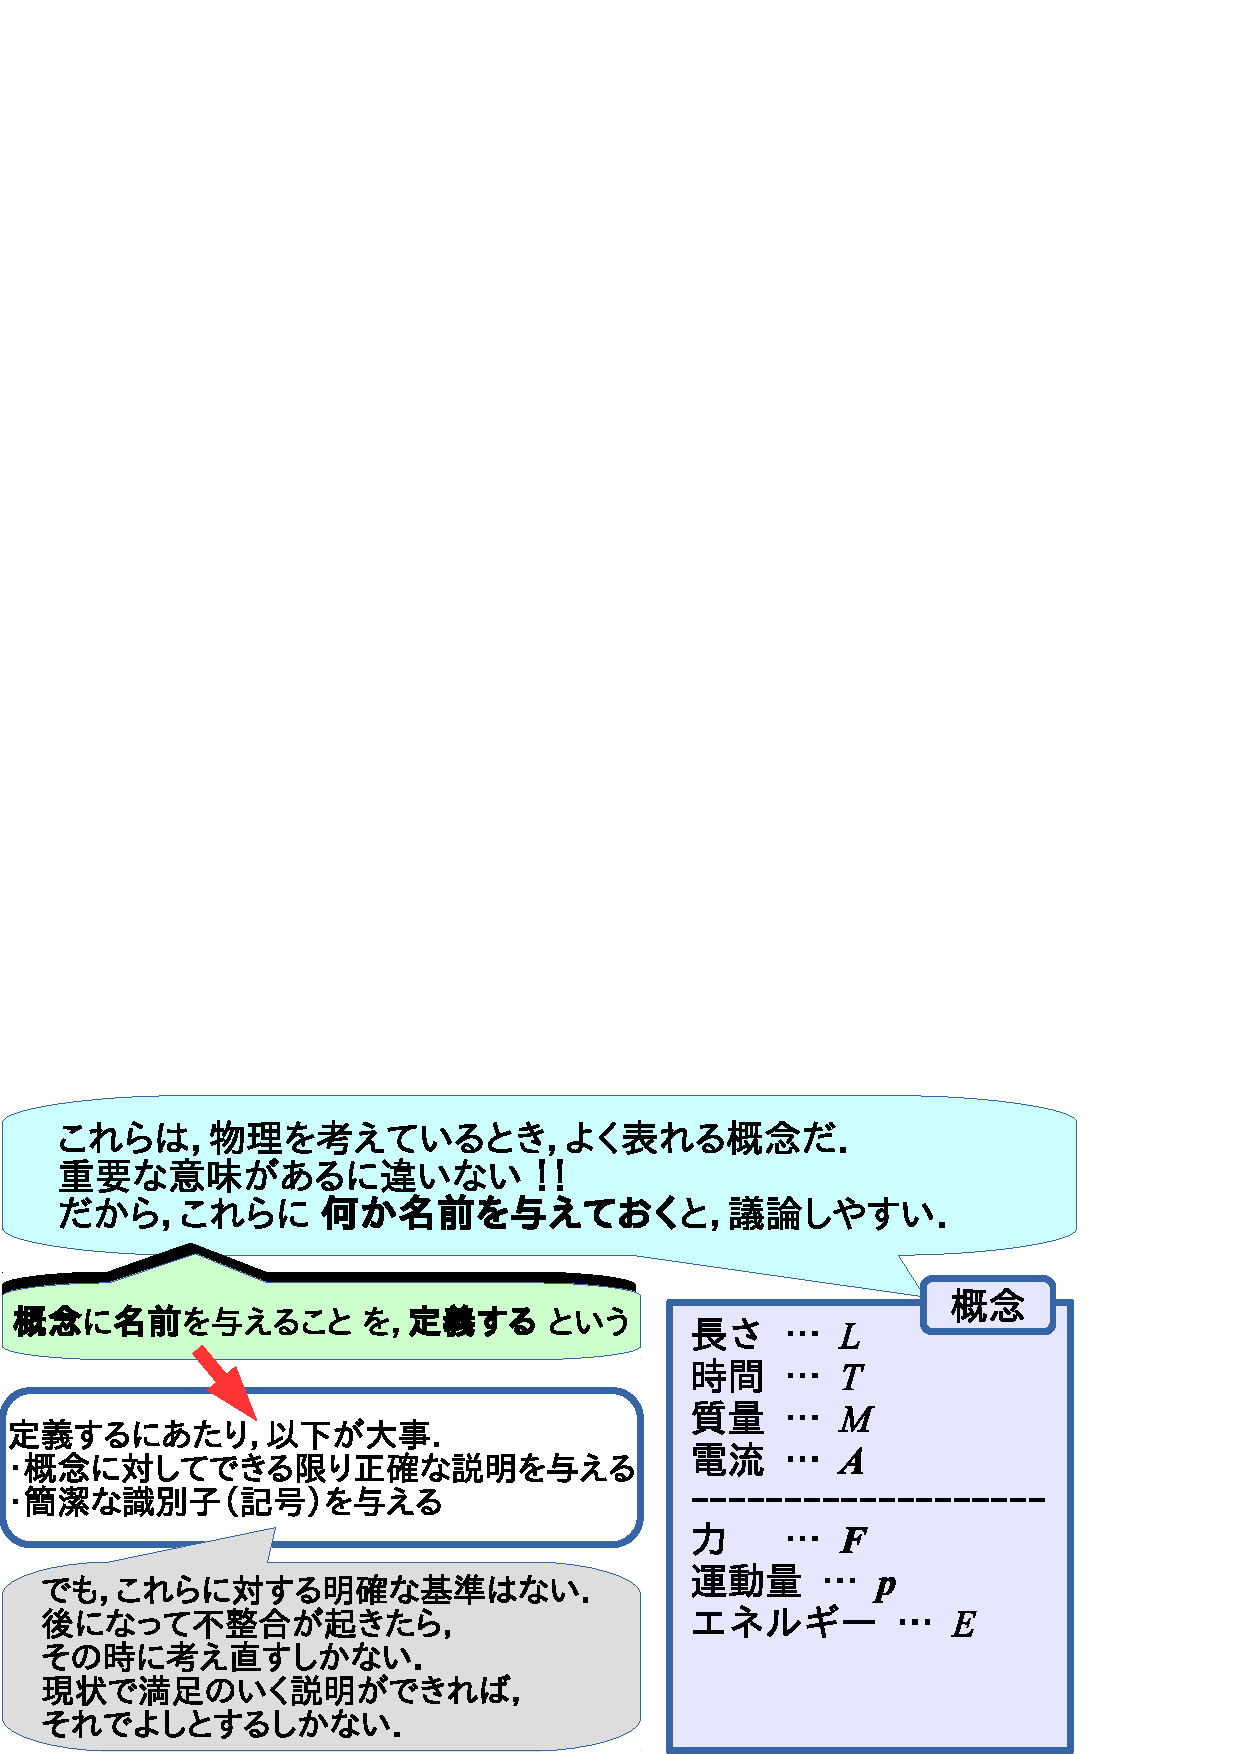
\includegraphics[keepaspectratio, width=6.5cm,height=4cm,clip]{teigi.pdf}
                            \caption{定義しよう!!}
                            \label{fig:teigi}
                        \end{center}
                    \end{figure}

                もちろん,定義した物理量が妥当でなかったと分かった場合,その定義を
                見直さなければならない.妥当でないというのは,実験事実と矛盾するこ
                とや,あるいは,全く的外れな定義等である.このようなことは,理論を
                作っていく上で必ず生じることであり,やむを得ない.

                このノートで定義される物理量は昔からその正しさが確認されているもの
                であり,従って,このノートで定義される物理量は今後も変化することが
                ないだろう
                    \footnote{
                        万が一,理論や実験技術の発展によって変更されることが余儀な
                        くされても,それは特殊な状況であるようなときに限って,定義
                        しなおされる.例えば,運動量  $\textit{\textbf{p}} = m\bv$ を
                        もつ物体はその速度が光速(光の速さ)に近いとき,相対性理論に
                        よってこの定義は見直される.詳細は,相対性理論の章を参照.
                    }.

                このノートでは「$\cdots$ と定義する」とは書かずに,「$\cdots$ という」
                と書くこともあるだろうが,これも定義のうちに入る と考えてもらいたい.

                また,物理量の定義を把握するためには演習が必要である.新しい概念が
                定義されたときは,演習書を用いてより感覚的に捉えられるようにしてお
                くとよい.先ほども書い通り,このノートで演習するようなことはない.

            \begin{memo}{「定義」の定義}
                「定義」という言葉の意味を,説明した.しかし,「定義」という語彙の
                定義をしたわけではない.単に,「定義」という難し言い回しを,噛み砕
                いて,言い直したに過ぎない.ならば,「定義」という語彙の定義は,
                どうなされるのだろうか,という疑問が浮かび上がってきたかも知れない
                    \footnote{
                        あるいは,ここの記述を読んで,疑問が提示され,不思議に思ったかもしれない.
                    }.


                しかし,実は,この疑問は意味のない疑問である.
                ゲーデールの定理などで有名な,自己言及が含まれていて,矛盾がおこるからである.
                「定義」という言葉を知らないと
                    \footnote{
                    ここでいう,「知る」という言葉は,
                    「定義」という語彙を,自分の頭で了解し,言葉で表せなくとも,感覚的に定義されている
                    ということを,念頭において使用した.
                    },
                「『定義』の定義とは何か」という疑問も起こりえない.
                一方で,「定義」という言葉の意味を知っているならば,そもそもこの疑問は起こりえない.
                    \footnote{
                        「『定義』の定義とは何か」とは何かという疑問をするためには,「定義」という言葉を
                        予め知っていないとならない.例えば,上の『定義』を一般的な語彙に拡張し,「Xの定義とは」
                        と置き換えてみるとわかりやすい.「Xの定義とは何か」と問うということは,すでに「定義」という
                        語彙を使用して疑問を投げかけているのであり,「定義」という語彙を了解した上での疑問と
                        いうことになる.そうなれば,X$=$「定義」とした時の,「『定義』の定義とは何か」という疑問を
                        投げるためには,やはり,予め「定義」という語彙を知っていないとなければならない.
                    }

                しかし,わからない.何をもって「定義」であると言えるのか.定義であるための基準とは
                何なのか.判断基準は定義と同じ意味であり,確かに,「『定義』の定義とは何か」という
                疑問と変わりなく思えるのだが,この疑問は自己矛盾を含んでいて,意味がないものである.

                私が今まで見てきた数学の解説書や参考書には,定義という言葉の意味を説明はされているものは
                あったが,定義であるための満たすべき基準が書かれたものは,見たことがない.

                どういうことだろうか.私の現在の解釈は,「定義」という語彙は名詞としてではなく,
                「定義する」という動詞として存在している,というものである.「定義する」という動詞は,
                ある語彙を,曖昧さなく
                    \footnote{
                        「曖昧」という語彙の意味も曖昧だ.ここでは,後の議論に論理的に相反する結果を
                        起こさない程度,と認識してもらいたい.
                    },
                より明確に意味づけを行う行為である,と考えるのだ.
            \end{memo}

%   %==========================================================================
%   %  Section
%   %==========================================================================
    \section{物理学の基本概念}
%       %======================================================================
%       %  SubSection
%       %======================================================================
        \subsection{物理量}
            物理的に意味のある量
                \footnote{
                    物理的に意味のある量とは,
                    「そのような量を導入することで現象がうまく説明できる」
                    という量である.
                }
            を \textbf{物理量} という.例えば,速度や加速度,重さ,長さ,時間などだ.
            運動量や力積,エネルギーや仕事量なども物理量である.実験により観測できる量
            は,すべて物理量であると思ってよい.

%       %======================================================================
%       %  SubSection
%       %======================================================================
        \subsection{物体}
            いままで,「もの」という表現を使っていたが,これからはもっとかっこよ
            く,\textbf{物体} ということにしよう.こっちのほうが,なんだか畏まっ
            てして,学問をしている感じになる.何でも難しく言えばいいということで
            はないのだけども,暗黙の了解をその言葉に含めるにはちょうどよいので
            ある.

            ここで,「物体」と表現したときに,暗黙の了解とされている性質を説明し
            よう.

            「もの」には,さまざまな性質がある.形,色,硬さ,におい等.また,そ
            の「もの」が食べ物であったなら,食感や味,風味もある.動物であれば,
            暖かさとか,おとなしいとか落ち着きがないとかなどの性格も,考えられる
            はずだ.一口に「もの」といってしまえば,こういう性質を全て考えなけれ
            ばならなくなる.けれど,これではあまりにも広い範囲の対象を相手にしな
            ければならず,一度に相手にするにはとても難しい
                \footnote{
                    難しい:不可能なことでない.「難しい」と表現されたときには,
                    原理的には可能なのであるが,実際に行うととても時間がかかる,
                    ということを意味している.例えば,「難しい問題」という表現が
                    ある.難しい問題とは,とくのに非常に時間のかかる(どれくらい
                    時間がかかるかは問題による)問題のことである.決して解けない
                    問題ではないのだ.まあ,そもそも「解けない問題」は問題ではな
                    い.だって,答えがないということがわかっているのだから(哲学
                    てきに難しい問題といわれたら,「“答え”のない問題」なのかも
                    知れないが).
                }.
            そこで,考える「もの」に制限を与えて,対象の範囲を狭くするのである.
            その制限とは,色とか,におい,味,食感,性格等は無視するということで
            ある.主に考えるのは,重さ,形,硬さである.どれに着目するかは,その
            つど異なるが,とにかく全ての性質を同時に扱うことは,難しいのでやらな
            い.

            特に,\textbf{物体} と言われたときには,「もの」の大きさと形しか考え
            ず,においとかの他の性質は全く考慮しないことを,暗に主張する.物理
            学でいう「物体」とは,日常生活で使用する言葉の“物体”とは異なる
                \footnote{
                    日常生活で使用する“物体”と同じ意味で,今まで「もの」と表現
                    していた.
                }.


%       %======================================================================
%       %  SubSection
%       %======================================================================
        \subsection{系}
            考える対象全体のことを \textbf{系} という.例えば,$N$ 個の物体の運動
            について考えるときに,「系全体」といわれたならば,それは,「$N$ 個の
            物体に関わるもの全て」ということ と同じ意味である.

            例えば,積み木が積まれている台車が運動しているとしよう.この台車がど
            のような動きをするのかを考えるとき,この積み木と台車の両方について考
            える必要がある.このときの系全体とは,「台車と積み木」である.太陽に
            対する地球の自転を考えるときの系全体とは太陽と地球のことである.より
            正確には周囲の他の惑星も系とすべきだ.要するに,今何を対象に考えてい
            るかとか,何に注目しているだとかの,そのような対象(もの)を総じて系と
            いうのだ.

%       %======================================================================
%       %  SubSection
%       %======================================================================
        \subsection{文字・数式・式変形}
            \begin{mycomment}
            物理学において,数式とは推論の道具に過ぎない.しかし,それは途方も
            なく有用な道具である.数式の持つ意味について,考える.
            \end{mycomment}

        \begin{mysmallsec}{文字}
            数式は文字で表現される.そして,文字は互いに関係付けられている.具
            体例で考える.ここに一冊の本があるとする.本には色々な性質が備わ
            っている.重さや色,紙の質,書かれている文字,匂い等,色々とある.
            物理学では,これら本のもつ諸性質のうち,特に関心があるのが,重さで
            ある.そこで,ここでは本の重さのみについて考えることにし,その他
            の性質(匂いやその記述されている内容)は全く無視してしまおう.それ
            で,本の重さについての記述をしたいのだが,どうすればよいだろう.
            なんて問うまでもなく,「重さを $W$ とおく」と表現すれば良い.「重さ
            を $W$ とおく」と表現したことにより,現実にある本の重さが,文字 $W$ で
            表現され,重さを数学的に扱うことが可能になった.視点を数式目線に変更
            して考えて見れば,文字 $W$ に重さという意味が与えられたとも考えるこ
            ともできよう.
        \end{mysmallsec}


        \begin{mysmallsec}{数と数字}
            ものの個数
                \footnote{
                    例えば,りんごの個数だとか,鉛筆の本数だとか,本の冊数だとか,
                    家の件数だとか,
                }
            や物の値段などで使われる,概念を抽象化したものを \textbf{数} という
                \footnote{
                    「スウ」と読む.「カズ」と読んでも間違いではないが,
                    数学をしている時には「スウ」と言う方が一般的.
                }.

            "数" を文字で表したものを \textbf{数字} という.同じ数に対して,
            いろいろな字が割り当てられていて,例えば,以下はすべて同じ数を示す文字である:
                \begin{equation*}
                    4 \,, \qquad \mbox{四} \,, \qquad \IV
                \end{equation*}
            数を表す文字は複数種類あり,どれを使っても良い.
            一般的に,\textbf{アラビア数字} と呼ばれる以下の数字が便利であり,多く使用される:
                \begin{equation*}
                    0 \, , \quad  1 \, , \quad  2 \, , \quad  3 \, , \quad
                    4 \, , \quad  5 \, , \quad  6 \, , \quad  \ldots
                \end{equation*}
            数式内の数字はアラビア数字を使う.文章内の数字はアラビア数字も使用するが,
            \textbf{漢数字} も使用する.漢数字とは,以下のような数字である:
                \begin{equation*}
                    \mbox{一}\, , \quad \mbox{二} \, , \quad \mbox{三}   \, , \quad \mbox{四} \, , \quad
                    \mbox{五}\, , \quad \mbox{六} \, , \quad \ldots
                \end{equation*}
            他にも,\textbf{ギリシア数字} ($\I$,$\II$,$\III$,$\IV$,$V$,$\VI$,$\ldots$) も数字だし,
            「正」の字を使って数えるときの途中段階の文字(記号?)も数字である.まあ,色々とあるが,
            物理学を勉強していく上では,上記のような常識的な範囲の数字の扱い方ができていれば十分である.
        \end{mysmallsec}

        \begin{mysmallsec}{変数}
            具体的な数($1,\,2,\,3,\,\ldots$)ではなく,"全ての数に対しての記述"をしたい場合がある
                \footnote{
                    数全般の性質を表したい場合は,具体的な数字を使って表現するわけににはいかない.
                    具体的な数字を使ってしまうと,その数にしか成り立たない記述になってしまう.
                }.
            そういった場合,\textbf{変数} という考え方を使う.
            全ての数に当てはまるということは,どんな数にも変わり得るということ.
            変数を表す記号は,様々である.
            中学や高校数学では,$x$ や $y$ や $z$ が使われる.また,$\theta$ や $\phi$ などの
            ギリシャ文字を使うことも多い.

            もっと高度な数学になると,
            変数が無限に多く欲しい場合があり.その場合は,アルファベットでは対応できない.だから,
            以下のように,アルファベットの右下や右上にアラビア数字を添えて,
                \begin{equation*}
                    {x}_{1} , \quad {x}_{2} , \quad {x}_{3} , \quad \ldots
                \end{equation*}
            と言った感じで,無限に変数を増産できる
                \footnote{
                    あるいは,
                    \begin{equation*}
                        {x}^{1} , \quad {x}^{2} , \quad {x}^{3} , \quad \ldots
                    \end{equation*}
                    でもよい.添字は右上でも右下でもどちらでも構わない.今のところは,
                    添字の位置には特に意味を与えていないが,後々(相対性理論を勉強する段階)では,
                    この添字の位置に意味を与えるので,注意が必要だ.
                }.
            添字は無限に増やせるからだ.だが,これでも,
            変数を無限に列挙することなどはできない.そこで,「$i$ は任意の自然数であるとする」という
            文言を添えて,
                \begin{equation*}
                    {x}_{i}
                \end{equation*}
            の一文字で済ますことが可能である
                \footnote{
                    $i$ には 1でも2でも99でも何でもよく,とにかく全ての自然数が順に与えられて,
                    整列させられているイメージを持って欲しい.そのイメージを具体的に書くと,${x}_{i}$ と
                    書かれた場合,
                    \begin{equation*}
                        {x}_{i}
                        \leftrightarrow
                        \left( 1,\,2,\,3,\,4,\,5,\,6,\,\ldots,\,i,\,\ldots,\,\infty \right)
                    \end{equation*}
                    ということである.$\leftrightarrow$ はその左側と右側で同じ意味を持つことを示す
                    ものである.

                    また,ここで,\textbf{無限} について定義せずに使用しているが,普段の
                    生活の意味の無限として捉えていて問題ない.無限を真面目に考え始めると,
                    深みにハマってしまい,議論が終わらなっくなってしまう.無限についての理解は
                    この程度で十分であろう:
                        \begin{equation*}
                            \mbox{無限大 とは,全ての数よりも大きい ということである.}
                        \end{equation*}
                        \begin{equation*}
                            \mbox{無限小 とは,全ての数よりも小さい ということである.}
                        \end{equation*}
                    "ということ" と表現したのには意味がある."という数" と書いていしまうと,
                    自己言及して矛盾になってしまう,「"全ての数" よりも大きい"数"」なんて
                    文は矛盾.だって,"全ての数"って言っているんだから,これよりも大きい数って,
                    全ての数以外の数だということになって,つまり,「"全ての数"以外の数」があることになる.
                    「"全ての数"以外の数」なんてものは矛盾.要するに,無限を数として扱ってはならない
                    ということである.
                }.

            変数の例を上げると,$f(x)=ax+b$ や $g(\theta)=\sin\theta$ と書かれた時の,
            $x$ と $\theta$ がそれに当たる.この場合の $x$ と $\theta$ は関数の定義域の全ての
            実数値を取りうることを意味付けられている.
        \end{mysmallsec}

        \begin{mysmallsec}{定数}
            ある特定の数(固定された値)であるが,それが特別な数ではない場合,これを \textbf{定数} という.
            読み方は,「ジョウスウ」または「テイスウ」である
                \footnote{
                    普通は「テイスウ」と読む.年齢を重ねた人が「ジョウスウ」と読む,という勝手なイメージがある.
                }.

            低すを表す記号として,アルファベットの最初の文字 $a$,$b$,$c$,$d$ などが使われる.大文字の $A$,$B$,
            $C$ が使われることも多い.変数に比べると,様々な文字が定数を表す記号として使われる傾向にある.
            ただ,教科書にはその都度,それが定数であるか変数であるかを説明しているので,どっちかわからずに混乱
            することはないだろう.

            先にも上げた例だと,$f(x)=ax+b$ とした場合の,$a$ や $b$ が定数である.
        \end{mysmallsec}

        \begin{mysmallsec}{整数(自然数,負の数),有理数}
            このノートでは,$0$ を含めた以下を \textbf{自然数} とよぶ:
                \begin{equation*}
                    0,\,1,\,2,\,3,\,4,\,5,\,6,\,7,\ldots
                \end{equation*}

            負の数とは,ある定数 $A$ に対して $A+x=0$ となるような $x$ のことをいい,$x:=-A$ と
            書く慣習がある.例えば,$A=1$ の時は,$x=-A=-1$ だし,$A=100$ だったら,$x=-100$ である.

            自然数と負の数を大きさ順に具体的に並べてみると,以下のようになる(右にあるほど大きい):
                \begin{equation*}
                    -4,\,-3,\,-2,\,-1,\,0,\,1,\,2,\,3,\,4\ldots
                \end{equation*}
            記号 $-$ のことを,\textbf{マイナス} とう.「負の数」という新たらしい数が作られたことで,
            今まであった0以外の自然数のことを \textbf{正の数} とよぶこともあり,記号は $+$ を使う.
            記号 $+$ は\textbf{プラス} という.「マイナス」と「プラス」は英語のplusとminusであり,
            "正"と"負"はこの英語に対して割り当てられた日本語語彙である.
            自然数と負の数を総称して,\textbf{整数} という.

            整数を2つ用意して(用意した2つが同じ整数でもいい)以下のように表した時,
            これを \textbf{有理数} という:
                \begin{equation*}
                    \frac{1}{2} \;,\;\; \frac{-9}{123} \;,\;\; \quad \frac{4}{-5} \;,\;\; \quad \frac{-9}{-177}
                \end{equation*}
            上記のように,真ん中に短い線を引いて2つの数を上下に記述した有理数の表現手法を \textbf{分数} という
                \footnote{
                    分数を一行で記述したい場合もある.こういう時は,1/2 とか -9/123 などと書く.
                    記号"/"を数の間に入れて分数を表現するのである.
                }.
            0 は下に書くことはできない
                \footnote{
                    0を下に書くと,四則演算で論理的に不整合な計算ができてしまい,体系に矛盾が生じる.
                    例えば,$\frac{1}{0}$ という数を書いてみる.
                    どんな数でも0をかければ,0になるので(これは0元の公理で,有無を言わずに認めることである),
                    $\frac{1}{0} \times 0 = 0$ となるのだが,この式の左辺は $\frac{1}{0} \times 0 = 1$ とも計算できる.
                    すると,$1=0$ となって論理的に不整合(矛盾)になる.矛盾が生じた理由は,
                    そもそも $\frac{1}{0}$ という数が存在すると仮定したからである.要するに矛盾を起こさないためには,
                    $\frac{1}{0}$ というような分母に0を置くような有理数(分数)を考えてはいけないということだ.
                }.
            また,上の数のことを \textbf{分子} といい,
            下の数のことを \textbf{分母} という.分子と分母の両方が負の数の時は,
            その両方のマイナスを取り去っても同じ分数としてあつかう:
                \begin{equation*}
                    \frac{-9}{-177} = \frac{9}{177}.
                \end{equation*}
            分母と分子のどちらか一方のみが負の数の場合は,負の分数として扱い,マイナス記号を
            分数の左真ん中へ移動させて書く:
                \begin{equation*}
                    \frac{-9}{123} = \frac{9}{-123} = -\frac{9}{123}.
                \end{equation*}

            分数の具体的なイメージは,割合だろう.全体の数を分母とし,分子には今注目している部分の数を書く.
            こうしてあらわされた分数は,注目している箇所は全体のどれくらいかを示す量となる
                \footnote{
                    あくまでも,分数を現実と対比させたい場合の例である.
                    数学では,このような具体的なイメージから発展させ,より抽象化される.
                    この例にとらわれると,マイナスの数が分母に書かれたときに,全体の数がマイナスになるが
                    どういうことだろうかと,無駄な考えに陥るかもしれない.数は現実の世界から必要に迫られて
                    人間が生み出したものであるが,数学ではそれを抽象化して数の性質を探求する学問である.
                    現実との具体的な対比に悩むのはナンセンスだ(物理学では大事なことだが).
                }.
        \end{mysmallsec}

        \begin{mysmallsec}{等号,不等号}
            2つの数を比較して,どちらが大きいか(あるいは小さいか)を文字で書きたいことがある.
            その場合,2つの数 $a,\,b$ を比較して,$a$ が $b$ よりも大きい場合は $a>b$ または $b<a$と書く.
            $b$ の方が $a$ よりも大きい場合は $a<b$ または $b>a$ とかく.$a$ と $b$ が
            等しい場合は $a=b$ とかく.記号にも名前があり,$=$ を \textbf{等号} といい,
            $<,\,>$ の2つを \textbf{不等号} という.不等号が2種類あると思われるかもしれないが,
            向きをどうするかの($a$ と $b$ の並べ方)違いであり,実際上,1種類記号である.
        \end{mysmallsec}

        \begin{mysmallsec}{演算,演算器号}
            演算には,「加算」と「乗算」がある.加算は記号 $+$ で表され,乗算は記号 $*$ で表される.
            加算と乗算はどういった計算かを一般的に示すことはできないので,以下に具体例を書くに留める.
            \begin{equation*}
                \mbox{加算: } 1+1=2 ,\quad 12=6+3+2+1
            \end{equation*}
            \begin{equation*}
                \mbox{乗算: } 1*1=1 ,\quad 36=6*3*2*1
            \end{equation*}

            加算と乗算以外にも,減算と除算があると思われるかもしれないが,減算と除算は加算と乗算の一部
            として含めることができる.減算の場合には,加算に対して負の数を導入することで,実現できる.
            つまり,
            \begin{equation*}
                \mbox{減算: } 1-1=1+(-1) , \quad 4=6+(-3)+2+(-1)
            \end{equation*}
            のように,減算ではなく負の数との加算だと解釈すれば,減算は加算のとみなせる.
            除算の場合には少し強引に聞こえるかもしれないが,分子を1とする分数と整数の除算,つまり,
            \begin{equation*}
                \mbox{除算: } 1 \divisionsymbol 2=\frac{1}{2}=1*\frac{1}{2} ,\quad 5 \divisionsymbol 6=\frac{5}{6}=5*\frac{1}{5}
            \end{equation*}
            と考えることで,除算を乗算の一部とみなせる.

        \end{mysmallsec}

        \begin{mysmallsec}{数式}
            世の中には非常に多くの本がある.本だけではない.鉛筆,ボー
            ルペン,コンパス,定規,机の上にあるものだけ上げても,非常に多くの
            ものが存在している.話を簡単にするために,机の上には,鉛筆と消しゴ
            ムと本がそれぞれ一つずつ存在し,これ以外のものは置いていないとしよ
            う.やはりこの3つのモノにも重さがあり,それを $W_{\mbox{鉛筆}}$,$W_{\mbox{消しゴム}}$,
            $W_{\mbox{本}}$ と表現することにしよう.これら3つの重さについて関心がある
            のは,それらの「関係」だろう.「関係」といったのは,どれが最
            も重いかとか,軽いかといったことである.この「関係」を数学的に扱
            うには,数式を使うと非常に簡単に表現できる.例えば,鉛筆の重さと消
            しゴムの重さが全く同じ時には,
                \begin{equation*}
                    W_{\mbox{鉛筆}} = W_{\mbox{消しゴム}}
                \end{equation*}
            と表現できることは,周知のことであると思う
                \footnote{
                    哲学的な疑問はここでは考えないことにしよう.数式は文字の羅
                    列である.ここで言うと,
                        \begin{center}
                            $W$,$=$,鉛,筆,消,し,ゴ,ム
                        \end{center}
                    という記号の羅列と捉えられる.文字の羅列になぜ意味を感じるの
                    か.うーん,難しい.とりあえず,この疑問は保留にしておこう.
                }.
            数式とは,文字と文字の「関係」を表現できるものである.
        \end{mysmallsec}

        \begin{mysmallsec}{式変形}
                        文字と数式には意味があり,特に物理学において文字と数式は,現実
            世界と強く結びついている.現実に起きている現象を数式で表すことが,物
            理学のひとつの方法なのだから.では,「式変形」に意味はあるのだろうか.
            結論から言えば,「式変形」それ自体にはなんの意味もない.単に,数学
            的に定義された文字の操作を行っているに過ぎない.にもかかわらず,「式
            変形」は非常に重要なのである.実際,式変形を行うことにより,いろいろ
            と推論を行うことができるし,また,それによって物理学が発展しているの
            である.意味が無いのに重要であるとは,いったいどういう事なのか.答え
            は,式変形を行うことにより,論理的必然性を確かめることができることに
            ある.何らかの意味をもった数式に式変形を施すことで,別の意味の数式を導出す
            る.これにより,正しい推論を行うことができるのである.世の中には論理
            的に矛盾したことは起こりえないから
                \footnote{
                    そもそも,論理的に矛盾していることを想像することもできない.
                    「ここに本があり,かつ,その同じ場所に本がない」という状況
                    を思い描くことが可能だろうか.
                },
            論理立てて考えることで,間違った結論を出すことは,ぐっと少なくなるは
            ずである.式変形を行うということは,論理的推論を行うということであり,
            そうして得た結論は,論理的に必然性を持つものであり,実験して確かめる
            価値は十分にあると言える.ちなみに,ここで言う必然性とは,物理学的に
            考えて必然ということであり,論理的に厳密に必然であることをいうのでは
            ない.物理学における論理的推論とは,「物理学的に考えてもっともらしい仮定」
            をもとにするため,この点において多少の厳密性が犠牲にされている.
        \end{mysmallsec}


        \begin{memo}{$a+b=b+a$ ?}
            $4+3=7$という足し算を考えよう.当然,$3$と$4$を入れ替えて書いて,$3+4=7$と書いても同じ.
            また,等号の右と左を入れ替えて,$7=4+3$あるいは,$7=3+4$としても,等式は成り立つ.
            本当にそうだろうか.$3+4$は$4+3$に同じなのか.実際のところ,違うだろう.
            3つのイチゴと4つのリンゴは,4つのイチゴと3つのリンゴとはことなる.
            確かに,個数だけに着目すれば$3+4=4+3$になるが,イチゴとリンゴの個数としての数字であると
            考える場合には,この等式は成り立たない.
            また,$3+4=7$という式を言葉にすると「3足す4は7である」と表現するのが自然であり,
            他方,$7=3+4$は同じように言い表すと「7は3足す4である」となる.両者の意味は全く違う.
            「7は3足す4である」は間違ってはいないが,決めつけているような表現であり,抵抗を感じる
                \footnote{
                    $7=5+2$でも,$7=1+6$でも,$7=10-3$でもよいのである.
                }.
            $3+4$も$4+3$も$5+2$も$10-3$も数式として考えれば,計算結果はすべて等しく,7である
                \footnote{
                    $3+4$という計算結果と,$4+3$という計算結果が等しく,両者とも互いに置き換えることが
                    できるということ.
                }.
            式計算する場合に,数や式に意味を考えてしまうと,余計なことを考え出してしまう(「$4+3$と$3+4$は同じか」とか).
            式計算時には数を抽象化してとらえなければならない
                \footnote{
                    きっとここら辺に数学の素晴らしさがあるのだろう.
                    こういう抽象化が興味深い体系的の数学を構成する基礎になっていくのだと感じる.
                }.

            一方で,物理学では単位という概念がある
                \footnote{
                    長さ[m],時間[s],質量[kg],電流[A]など.
                }.
            物理学で扱う数字には意味が込められており,計算時に単位を意識する必要がある.
            単位が違う数字の足し算は認められていない
                \footnote{
                    長さ1[m] + 質量1[kg] という計算は全く意味不明だ.
                }.
            掛け算は認められている
                \footnote{
                    だからこそ,新しい概念を作ることができる.
                    エネルギーの単位[J]は,力1[N]と長さ1[m]の積として定義されている.
                    ($[\mbox{J}] := [\mbox{N} \cdot \mbox{m}].$)
                }.
            単位は数学にはない概念である
                \footnote{
                    ここにも,科学と数学の違いが表れている.
                }.
            物理学で数式を扱う場合,数学と全く同じように扱ってしまうと,
            単位の違う数字の足し算をしてしまうという誤りをしがちである.
        \end{memo}



%===================================================================================================
%  Chapter : 力学の基本概念
%  説明    : 力,重ね合わせの原理,力(作用)の種類,単位などの基礎概念について説明する.
%===================================================================================================
\chapter{力学の基本概念}
%   %-----------------------------------------------------------------------------------------------
%   %  Input
%   %    File Name : PhysNote_CM_MechIntro.tex
%   %    説明      : 物理学の基本的な考え方(定義,法則等)について説明する.
%   %-----------------------------------------------------------------------------------------------
%===================================================================================================
%  Chapter : 力学の基本概念
%  説明    : 力,重ね合わせの原理,力(作用)の種類,単位などの基礎概念について説明する.
%===================================================================================================
%   %==========================================================================
%   %  Section
%   %==========================================================================
    \section{力とその性質}
%       %======================================================================
%       %  SubSection
%       %======================================================================
        \subsection{力(ちから)}
            世の中には,\textbf{力} といわれる現象がある.この「力」は様々な意味
            合いで使用される.視力,脚力,握力などの身体能力に関する「力」.計算
            力,想像力などの思考に関する「力」.ほかにも,技術力,接客力,情報収
            集力,対応力など,人の性格や能力に関する「力」などいろいろ考えられる.

            物理学で対象とする \textbf{力} は,弾性力や反発力,物体を変形させる力,
            物体の運動方向を変化させる力などである.以下,「力」と表現される場合
            には,特に断りのない限り,このような力を想定する.

            力とは,捕らえ所がなく,非常に曖昧である.現に,ニュートン力学では,
            力とは何かを説明することはできない.では,どのように力というものを
            考えるのか.結論から言うと,力の存在を,なんの根拠もなしに認めること
            である.力という物理現象の発生原因が分からないのだけど,実際に,
            私たちは日常的に,力が存在しているということに関して,疑いを持つこと
            はない
                \footnote{
                    力の存在に疑問をもつこともあることだろう.しかし,ここ
                    では哲学について語っているのではない.力とは何か,も
                    っと言うと,力という現象を感じる私たちとは何なのか,こ
                    れはひどく難しい問題である.なので,こういう問題には目
                    を閉じておくことにしよう.今の私の興味は,世界がどのよ
                    うに構成されているかということであり,こんなところで,
                    足を止めてしまってはならない.知りたいことはもっと先に
                    ある.そのために,力という現象の存在を素直に認めること
                    にしよう.ただし,この問題を忘れてはならない.ノートの
                    端の方に,「力とは何か」という疑問をメモしておこう.
                }.

            しかしながら,力は重要な概念である.
            力学の最大の目標の一つは,物体の運動の軌道を求めることにある.
            それには,物体にかかっている力を,考えないとならない.
            物体の運動の原因は力であり,力は
            物体の運動を解析する上で,非常に重要なものである.

            これだけ重要な概念である“力”なのだけど,「力とは何か」と問われると,
            回答するにはとてもむづかしい
                \footnote{
                    素粒子物理学の教科書などでは,(ゲージ粒子を介した)「相互作用」と
                    説明されるが,詳細は,素粒子物理を考えるときに説明しよう.
                }.
            とりあえずの力の説明として,物体を変形させる,あるいは,物体の位置を
            変化させる原因としておこう.言い換えると,物体が変形すれば,その物体に
            力が加えられたということになるし,物体の位置が変化したならば,この場合にも
            物体に力が加えられたということになる.

            物体の変形や変位を説明する概念として,力の存在が要請されるとしてもよい.

%       %======================================================================
%       %  SubSection
%       %======================================================================
        \subsection{力の重ね合わせの原理}
            複数の力が物体に働いているとき,その力を合計することを,
            力の \textbf{合成} という.合成された力のことを \textbf{合力} という.
            力の合成は,ベクトル和 で表現できる.すなわち,物体に $N$ 個の力が加わっているとき,
            その合力は,
                \begin{align}
                    \bF_{\mbox{合力}}
                    = \bF_{1}+\bF_{2}+ \cdots + \bF_{N}
                \end{align}
            である.和の記号を用いると
                \begin{align}\label{gouryouku_gouryoku}
                    \bF_{\mbox{合力}} = \sum^{N}_{i=1} \bF_{i}
                \end{align}
            のようにかける.

            また,逆に,1つの力を,複数の力の合力である
                \footnote{
                    式(\ref{gouryouku_gouryoku})は等式であり,
                    左右が等しいのだから明らかではあるが,
                    少しだけ気付きにくいかと思われたので書いておいた.
                    すなわち,1つの力を複数の力に \textbf{分解} することもできる.
                    }.
            力の分解は,よく行われる.例えば,$x-y$ 平面上における力を表現するのに,
            力を $x$ 方向と $y$ 方向に分けて考えることが多い.
                \begin{figure}[hbt]
                    \begin{center}
                        \includegraphics[keepaspectratio, width=6cm,height=6cm,clip]{f_bunkai.pdf}
                        \caption{力の合成,力の分解}
                        \label{fig:f_bunkai}
                    \end{center}
                \end{figure}

            力学では,力が重ね合わせの原理を満たす理由は問わない.
            この原理は,実験的に確かめられる法則として扱われている
                \footnote{
                    もしかしたら,将来,このことを説明できる日が来るかもしれないが,
                    今はこれを説明できるだけの知識がない.ただ,電磁気力に関していえば,
                    電磁場の線形性に帰着できる(問題を先送りしただけ,かもしれないが).
                }.

            別称として,\textbf{平行四辺形の法則},\textbf{力学の第0法則} とかと表現されることもある.
            重ね合わせの原理が成り立つことを,数学的に表現すると,「力には \textbf{線形性} がある」ともいえる.
            もっと物理学の学習を続けていけば,力の重ね合わせの原理を
            説明できるようになるのかもしれない.しかし,ここではその理由はわからないので.
            とりあえず,重ね合わせの原理を認め,学習を先に進めるべきだ.

              \begin{memo}{和の記号: $\sum$}
                例えば任意の4つの実数 $a_{0},\,a_{1},\,a_{2},\,a_{3}$ が与えられたとする.
                この時,$a_{0}$ から $a_{3}$ までの和 $S$ を書き表すとき,
                  \[
                    S = a_{0} + a_{1} + a_{2} + a_{3}
                  \]
                のように書き表せる.しかし,項数が9999個になった場合($a_{1},\,a_{2},\,\cdots\,a_{9999}$ ),
                書き表すことはできない
                  \footnote{
                    原理的には可能であるが,実際に書くのに時間がかかるため現実的ではない.
                  }.
                そこで,$a_{0}$ から $a_{9999}$ までの数の合計を計算することを示す記号を導入したくなる.
                和の記号として,$\sum$ を新たに導入し,以下のように記述することにしよう.
                  \[
                    \sum^{9999}_{i=0} a_{i} := a_{0} + a_{1} + a_{2} + \cdots + a_{9999}.
                  \]
                $\sum$ は「シグマ(Sigma)」と発音する.
                今の例だと上限が9999の場合に限ってしまうが,上限を任意の数 $N$ として場合には,
                次にように書く
                  \footnote{
                    前の例だと具体的な数字だった9999を $N$ という文字に変更する.
                  }.
                  \[
                    \sum^{N}_{i=0} a_{i} := a_{0} + a_{1} + a_{2} + \cdots + a_{N}.
                  \]
                さらに,この例だと最初の数字は0であるが,もちろん任意でよい.
                最初の数を $m$ と文字で置き換えて($m<N$であるはず),
                  \footnote{
                    例えば,$a_{0},\,a_{1}$ がべっと定まっていて,この2つの数にさらに
                    $a_{2}$ から $a_{N}$ までの数の合計を足したいこともありうる.
                  }
                  \[
                    \sum^{N}_{i=m} a_{i} := a_{m} + a_{m+1} + a_{m+2} + \cdots + a_{N}.
                  \]
                  これで,項数が多くなっても和を書き表せるようになった.

                  ちなみに,$a_{i}$ の添え字 $i$ は和の具体的な計算(和の記号の展開)の時に,
                  失われてしまう数で\textbf{ダミー}の数字と言われることがある.別に $i$ ではなく,
                  $j$ を使ってもよい.
                  その場合は以下のようになるが,$i$ の場合と意味は同じである.
                  \[
                    \sum^{N}_{j=m} a_{j} := a_{m} + a_{m+1} + a_{m+2} + \cdots + a_{N}.
                  \]

                  項数を無限大 $\infty$ にした場合でも,
                  \[
                    \sum^{\infty}_{j=m} a_{j} := a_{m} + a_{m+1} + a_{m+2} + \cdots
                  \]
                  と形式的に表現することもできる
                    \footnote{
                      「形式的に」といったのは,$\infty$ が数ではないために,正式な和の手続きに
                      なっていないからである.しかし,この表現により,無限にある項数を順に足し合わせる
                      という行為をイメージさせることが可能である.
                    }.
              \end{memo}


%       %======================================================================
%       %  SubSection
%       %======================================================================
        \subsection{作用}
            力のことを,場合によっては,\textbf{作用} ということもある.
            例えば,「2つの物体間に働く相互作用」と書かれていたら,
            これは,2つの物体に働く力という意味である
                \footnote{
                    量子力学や素粒子理論,あるいは,一般相対性理論の教科書でよく使われる表現だ.
                    ニュートン力学でも,「作用$\cdot$反作用の法則」のように使用されれる.
                }.

            宇宙論や素粒子理論の教科書などでは,その冒頭に「力には4つの種類ある」
            と紹介さることが多く,\Table\ref{table:f4force} が掲げられる
                \footnote{
                    当然ながら,この力の分類は,物理学の発展により得られたものであり,
                    最初から知られていた事実ではない.
                }
            この4つの力は,それそれで従っている物理法則や性質が異なる.
            つまり,少なくとも4つの物理法則があるということであり,
            だけどこれは,物理法則はただひとつであるという物理学の精神に反する.
            物理学の理論構築の目標の一つは,この4つの力を自然に説明することである.
            要するに,4つの力を説明できるような,もっと大きな理論的枠組みを構成し,
            その枠組みの中で4つの力が自然に導かれるような理論を作りたいのだ
                \footnote{
                    今では,電磁気力と弱い相互作用と強い相互作用の3つの力を説明できる
                    統一理論が知られいて,これを \textbf{標準模型} という.しかし,
                    標準模型には人為的な定数が多く含まれており,また,万有引力も
                    説明できないので,私達が知りたい力の統一理論ではない.

                    当然ながら,力を統一的に説明できるという保証はどこにもない.
                    統一理論の確立は可能であると信じて,理論を作り上げる努力をするしかない.
                    超弦理論は,現状での最も有力な理論の1つであるが,超弦理論を実験的に検証されていない.
                    他の候補にもループ量子重力という理論も提案されているが,こちらも実験検証ができていない.
                    一般に周知される理論の確立にはまだ時間がかかるようだ.
                    もしかしたら,その過程で,力を統一的に説明できない,という結論に至る可能性もある.

                }.

                 \begin{table}[htb]
                  \centering
                  \caption{4種類の力}
                  \begin{tabular}{|l|c|}           \hline
                    名称         & 別称         \\ \hline  \hline
                    万有引力     & 重力         \\ \hline
                    電磁気力     & ローレンツ力 \\ \hline
                    弱い相互作用 & $\beta$崩壊  \\ \hline
                    強い相互作用 & 核力         \\ \hline
                  \end{tabular}
                  \label{table:f4force}
                \end{table}

            \begin{mysmallsec}{万有引力(重力)}
            万有引力はどんな物質も持っている性質で,その強さは,4つの内で最弱.
            重力とはが物を引っ張る力のことで,それは万有引力の一部であるが,
            重力という表現のほうが実感があり馴染み易いせいか,万有引力と同義的に
            使われることが多い.一般的に,万有引力と重力は同義であると考えてよい
                \footnote{
                    ただし,両者を区別して考えたい場合もあるので,文脈により判断したい.
                }.

            重力を説明する理論は一般相対性理論である.重力があまり強くない場合は,
            ニュートンの力学で十分精度よく説明される.
            \end{mysmallsec}

            \begin{mysmallsec}{電磁気力(ローレンツ力)}
            電磁気力は,ローレンツ力と言われることもある.ローレンツは電磁気現象の
            解明に貢献した物理学者の名前である.電磁場中を運動する電荷が受ける力の
            ことである
                \footnote{
                    詳しくは電磁気学の部分で学習する.
                }.

                        電磁気力は電磁気学,あるいは,電弱統一理論によって説明される.
                        電弱統一理論は電磁気力と次に説明する弱い相互作用の両方を説明できる理論である.
                        ただ,電磁気力のみを考える際には,マクスウェルの古典的な電磁気学
                        で十分な場合が大半.
            \end{mysmallsec}

            \begin{mysmallsec}{弱い相互作用}
            弱い相互作用とは,原子が$\beta$崩壊するときに使われる力である.原子核や
            素粒子を扱う場合に,重要な力だけれど,力学では対象範囲外の概念である.
            量子力学や特殊相対性理論(場の理論)によって説明される力である.
                        電弱統一理論によって説明される.
            \end{mysmallsec}

            \begin{mysmallsec}{強い相互作用(核力)}
            強い相互作用とは,原子核を構成する陽子と中性子を結びつける力である.
            陽子と陽子,中性子と中性子も強い相互作用によって引き合っている.
            電磁気力を考えると陽子同士は反発しあって安定しないのだが,この
            強い相互作用によって引き合うために,原子核が安定して存在できる
            だから,当然,強い相互作用は電磁気力よりも強い力である.しかし,
            単純にそう考えると,電磁気力は強い相互作用に隠されてしまう(
            表だって電磁気力を感じなくなってしまう)はずだが,実際はそうではない.
            その理由は,有効範囲の違いで説明される.原子核よりも狭い領域では
            強い相互作用が優勢であるが,原子核以上の範囲では強い相互作用は
            電磁気力よりも弱くなるのだ.
                        各力は,量子色力学によって説明される.
            \end{mysmallsec}

%       %======================================================================
%       %  SubSection
%       %======================================================================
        \subsection{外力}
            系の外から生じる力が系に影響を及ぼすこともあろう.対象とするもの以外
            から受ける力のことを \textbf{外力} という.例えば,重力に
            逆らって物体を持ち上げるときに,人間による力が必要である.物体が勝手
            に重力に逆らって宙に浮いたりすることはありえないからである.このよう
            に,人間による力を想定して,外力という言葉を使うこともある.

%   %==========================================================================
%   %  Section
%   %==========================================================================
    \section{基本単位 ([s]/[m]/[kg]/[A])}
%       %======================================================================
%       %  SubSection
%       %======================================================================
        \subsection{単位と測定}
            物理学は経験・実験結果がその基礎であることは前に書いた通りである.
            実験とは,実験すべき対象に何か刺激を与えて,その反応をみることである.
            このとき,対象の持っている何らかの量を測る必要が出てくる.ここで,「
            「測定とは何か」ということを考え直さないといけない.
            答えは簡単だ.
            \textbf{測定とは,基準値に対して何倍であるかを調べる行為である}と言える.
            言い方を変えれば,測定基準と測定対象の大きさを比較することである.
            測定対象は色々とあるが,例えば,音の大きさだったり,気圧,
            紐の長さ,ものの色,糖度,$\cdots$ etc,と色々ある.
            この比較対象となる基準値は,\textbf{単位} と呼ばれる.
            「基準値」という語彙は意味が広く,合格基準点とかのボーダーライン的な
            意味でつかわれることも多い.単位という特別な名称を与えたのは,基準値
            の意味を狭めるためである.単位とは,測定対象の大きさや量を数字で示す
            ための,最も基本的な大きさを規定するものである.

        \subsection{4つの基本単位}
            物理学では,以下の4つを,測定可能な最も基本的な量としている(\Table\ref{table:f4unit})
            \footnote{
                逆に言うと,この4つの単位は,他から導くことのできない単位である.
                いわば,単位系におけるもっとも素朴な要素となる.単位の素粒子的な
                役目を担っている.他の単位は,これらの単位から組み立てることが
                できる,というか,そのように定義される.
            }.
                \begin{table}[htb]
                  \centering
                  \caption{基本単位(物理学の基本4単位)}
                  \begin{tabular}{|l|c|c|l|}                  \hline
                    名称 & 記号   & 英字表記  & 読み       \\ \hline  \hline
                    時間 & [s]    & second    & セカンド   \\ \hline
                    長さ & [m]    & meter     & メートル   \\ \hline
                    質量 & [kg]   & kilo-gram & キログラム \\ \hline
                    電流 & [A]    & ampere    & アンペア   \\ \hline
                  \end{tabular}
                  \label{table:f4unit}
                \end{table}

            この4種類の単位が,現在の物理学の \textbf{基本単位} である.
            これらは,国際単位系であるSI基本単位に指定されている.
            ちなみに,SI単位系には,これら4つほかに,以下の3つが挙げられている(\Table\ref{table:o4unit}).
                \begin{table}[htb]
                  \centering
                  \caption{他の基本単位}
                  \begin{tabular}{|l|c|c|l|}                      \hline
                    名称       & 記号   & 英字表記 & 読み      \\ \hline \hline
                    熱力学温度 & [K]    & kelvin   & ケルビン  \\ \hline
                    物質量     & [mol]  & mol      & モル      \\ \hline
                    光度       & [cd]   & candela  & カンデラ  \\ \hline
                  \end{tabular}
                  \label{table:o4unit}
                \end{table}

            しかし,熱力学を考える場合の熱力学温度[K]を除き,
            物理学的観点からは,この3つは基本単位とは考えない.
            物質量の[mol]は化学における重要な単位であるが,
            これは,統計物理学から定義できる量である.
            また,光度[cd]は光の強さを表している.電磁気学により,
            光は電磁波であることが示されており,その強さは電磁波の
            波長(もしくは周波数)で表せる.さらに言うと,実は熱は現実には存在しない.
            熱は,統計物理学によって,多数の分子の乱雑な運動であると説明される.
            つまり,日常で感じている熱とは,分子集団の持つ運動エネルギーであると
            言い換えられる.なので,これらの3つの単位は,他から導くことが
            できるという点で,物理学の基本単位としては,扱われていない.
            もちろん,基本単位でないからと言って,無意味ということではない.
            現象を簡潔に説明できる場合には,この3つの単位も積極的に使用される.

%       %======================================================================
%       %  SubSection
%       %======================================================================
        \subsection{組立単位}
                その他の単位として,例えば,角度を表現する[rad]や,光の強さを表現する[cd]
                などがある.角度は長さと同じに扱えるが,実際のイメージに即して考える場合に,
                欠くことのできない単位である(非常に便利であるという意味で).

                また,力やエネルギーの単位は,基本単位で構成される \textbf{組立単位} である.
                例えば,力の単位は[N](「ニュートン」と読む)であり,これを基本単位に
                分解すると,
                \begin{equation*}
                    [\mbox{N}] = [\mbox{kg}\cdot\mbox{m}/\mbox{s}^{2}]
                \end{equation*}
                となる
                    \footnote{
                        日本語による読み方は,
                        「キログラム メートル 毎秒毎秒(まいびょうまいびょう)」である.
                    }.
                エネルギーの単位[J](「ジュール」と読む)は,
                \begin{equation*}
                    [\mbox{J}] = [\mbox{Nm}] = [\mbox{kg}\cdot\mbox{m}^{2}/\mbox{s}^{2}]
                \end{equation*}
                    \footnote{
                        日本語による読み方は,
                        「ニュートン メートル」である.
                        基本単位に戻ると,
                        「キログラム メートル二乗 毎秒毎秒(まいびょうまいびょう)」となる.
                    }.
                力やエネルギーの性質などについては,後で学習する.ここで覚えておくべきことは,
                後の学習で現れる全ての物理量は,4種類の基本単位から組み立てられているということ
                である.

%       %======================================================================
%       %  SubSection
%       %======================================================================
        \subsection{測定の方法}
            測定とは,測定対象の大きさを知るための行為である.物体が大きいとか,小さい
            とかという判断は,どのように行うべきだろうか.例えば,単に大きな
            消しゴムとか,小さい鉛筆とかと言ったところで,具体的な大きさを思い
            描くことは不可能である.確かに,これまでの経験から常識的な大きさを
            思い描いて,これと比較することで,大きいだとか小さいだとかというこ
            ともある.しかし,これは日常生活でのはなしであって,物理学において
            は,このような曖昧さは避けるべきだ.常識的な大きさと言われても,
            その思い描く大きさは人それぞれだし,ましてや常識的な大きさよりも大
            きいと表現されてしまっては,具体的な大きさは全く想像がつかない.

            では,物の大きさを具体的に,しかも誰にとっても同じような大きさが想
            像できるように表現するには,どうしたら良いだろうか.答えはもう出て
            しまっている.\textbf{単位} という概念を導入するのである.単位とい
            う概念を導入することで,物体の大きさを具体的に表現できる
            ようになるのだ.

            例えば,ここに2つの異なる長さの棒があるとしよう.簡単のため,この2
            つの棒はまっすぐであるとする.2つの棒は長さの違いで区別することがで
            きて,長い方をA,短い方をBとしよう.今,何も考えずに“長い方”ある
            いは“短い方”と書いてしまったが,どのように長さを測ったのだろうか.

%       %======================================================================
%       %  SubSection
%       %======================================================================
        \subsection{単位}
            \textbf{単位} とは,測定の基準のことである.物理学は,物体の長さ
            や重さ,時間,電流値を最も基本的であるとしている.そして,力学では,
            この内の三つ,すなわち,\textbf{時間}$\cdot$\textbf{長さ}$\cdot$\textbf{重さ}
            を特に重要視する.これらはすべて実験的に観測されるものである.単位
            の重要性について,より具体的に「大きい」という言葉を例に取り,以下
            に説明してみよう.


%       %======================================================================
%       %  SubSection
%       %======================================================================
        \subsection{時間}
            時間の進みは,あらゆる空間において,一定である.時間を $t$ で表す.
            時間の単位を [s] で表す.「second」 又は 「秒」 と読む.
            時間は 過去$\rightarrow$現在$\rightarrow$未来 と進むと考える
                \footnote{
                    ここで注意しておく.今までのところ,
                    未来$\rightarrow$現在$\rightarrow$過去という風に,
                    私達が実感している時間の向きとは
                    逆の向きに時間が進んでも,物理法則が矛盾するようなことはない.
                    但し,熱力学の第2法則(「エントロピー増大の法則」:$\leftarrow$後述)は,
                    この限りではない.
                }.
            \begin{myshadebox}{単位時間(1[s])の定義}
                「${}^{133}${\rm Cs} 原子が出す電磁波が 9192631770 回振動する時間」が1[s] と定義される.
                原子の振動回数を数えることで1秒を測るということである.
            \end{myshadebox}

            \begin{memo}{“時間”と“時刻”の違い}
                ここで,「時間」と「時刻」の違いを確認する.
                言葉よりも,図で示したほうが早い(図\ref{fig:jikoku-to-jikan}).
                \begin{figure}[hbt]
                    \begin{center}
                        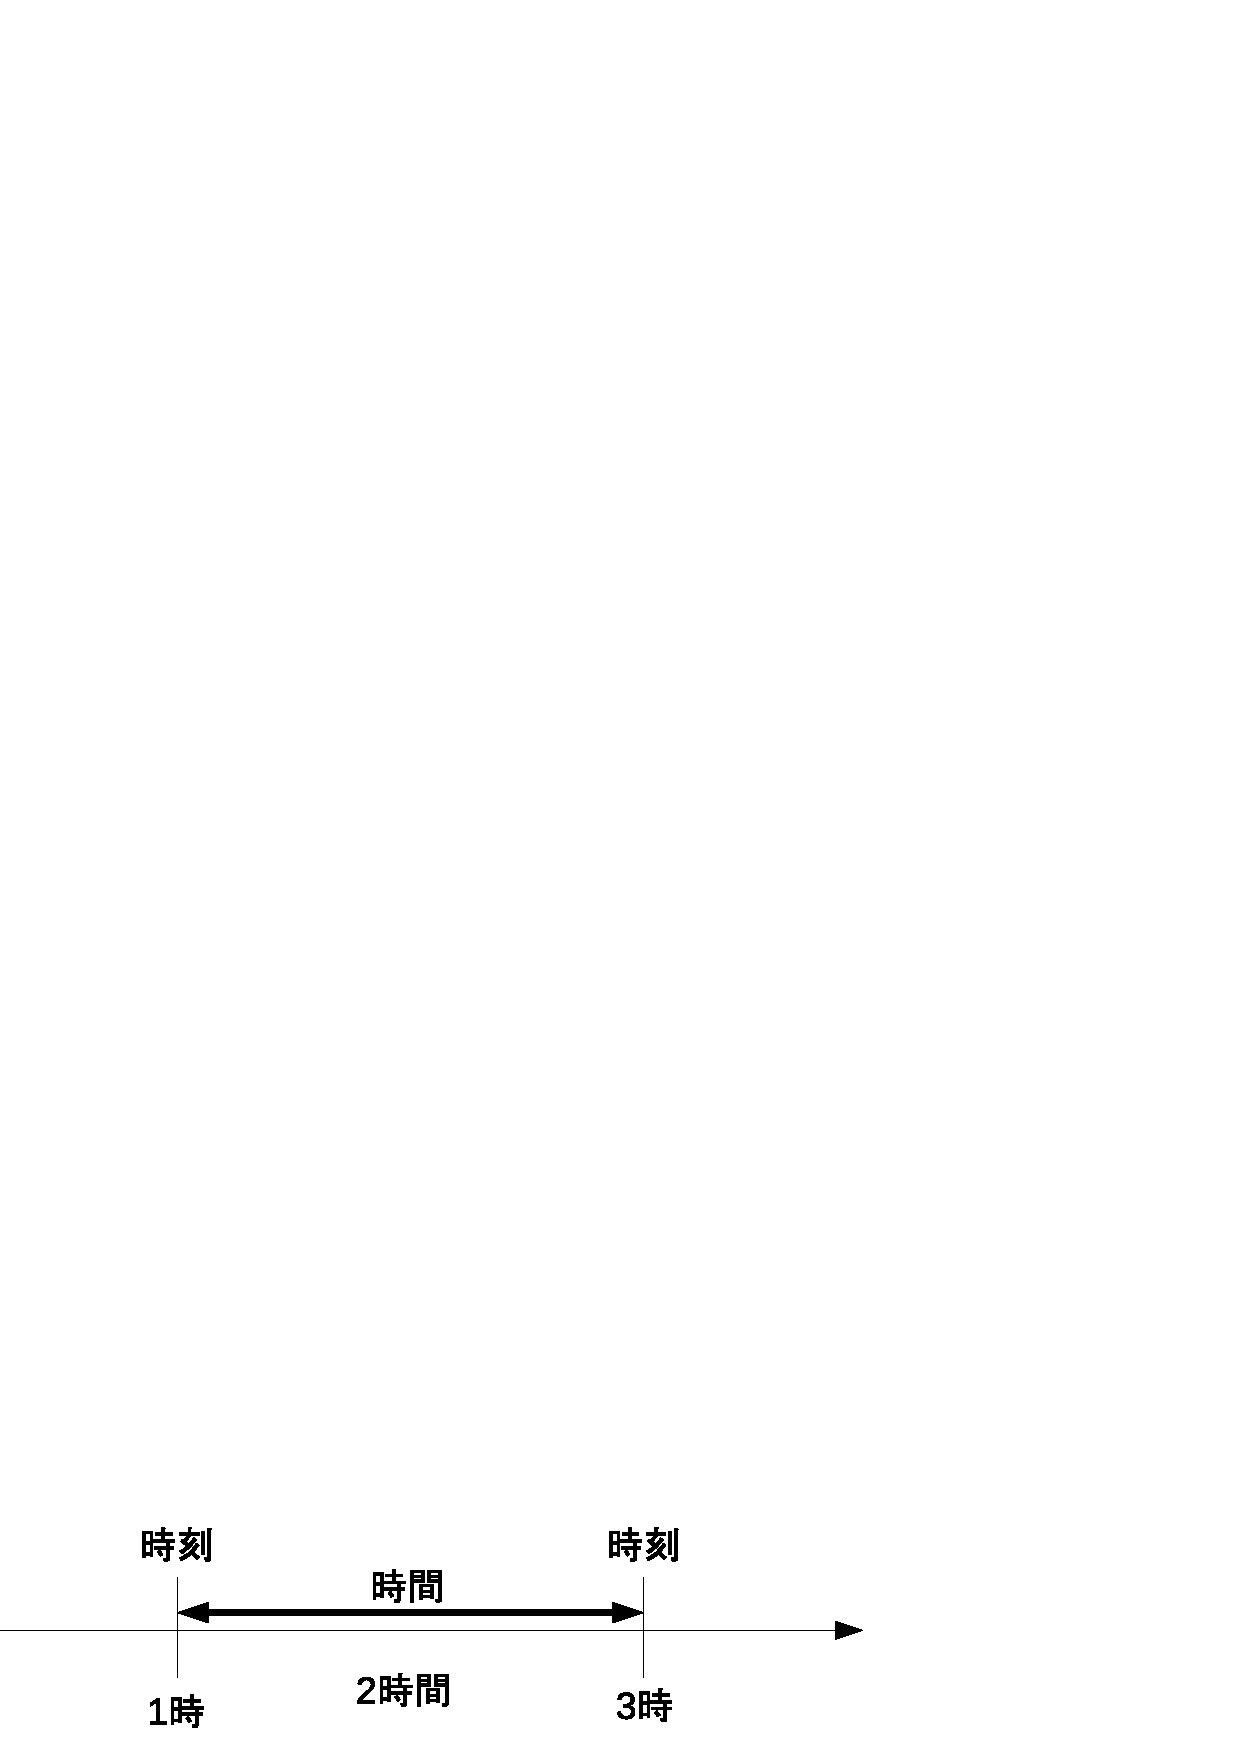
\includegraphics[keepaspectratio, width=7.2cm,height=3.6cm,clip]{jikoku-to-jikan.pdf}
                        \caption{時間と時刻}
                        \label{fig:jikoku-to-jikan}
                    \end{center}
                \end{figure}

                例えば,「1時から3時までの時間は2時間である.」という主張をするとき,
                この“2時間”が \textbf{時間} であり,1時とか3時は \textbf{時刻} である.
                時刻は幅がなく,時間を直線で表現にしたときには,点で表現される.
                それに対して,時間はある時刻と別の時刻の間の間隔である.

                勘違いを起こしがちなことがある.それは,
                すべての時刻を集めたものが時間である,という考えである.
                しかし,これは間違いだ.
                時間は数直線で表すことができ,よく,\textbf{時間軸} と
                いう言葉で表現される.時刻とは,時間軸の一点を表す語彙であるが,
                その一点には幅はない.つまり,時刻の時間は0である.0をいくらたくさん
                足しあわせたところで,結果は0であることは言うまでもない.
            \end{memo}

            \begin{memo}{飛ぶ矢のパラドクス}
                エレアのゼノン
                    \footnote{
                        $Z\eta \nu \omega \nu$(B.C.490 -- B.C.430, 古代ギリシア):
                        ギリシャ文字をそのままアルファベットに変換すると「Zhenon」.
                        しかし,英語表記で「Zeno」(ラテン語,フランス語でも同じ)で,
                        ドイツ語表記では「Zenon」と表される
                        (ドイツ語の場合,「ツェノン」と発音するのかな).
                        「エレアのゼノン」とも言われる.古代ギリシャ人.
                        ちなみに,「キプロスのゼノン」と呼ばれる,同名の人物がいるが,
                        その人とは別人.「エレアのゼノン」と書いたのも,それと区別するため.
                        キプロスのゼノンも,大哲学者であり,
                        ストア派と言われる禁欲的な態度や特を重んじる思想や態度を唱えた.
                    }
                は,次の4つのパラドクスを考えだしたことで,有名な人物である.
                    \begin{enumerate}
                        \item 二分割のパラドクス
                        \item アキレスと亀のパラドクス
                        \item 飛ぶ矢のパラドクス
                        \item 競技場のパラドクス
                    \end{enumerate}
                この内,3番目の「飛ぶ矢のパラドクス」が時間に関するパラドクスである.
                このパラドクスは,次のようなものである.動いている物体といえども,ある瞬間
                には,定まった1つの位置に位置しているはずである(写真をとるとその一点に位置している).
                定まった位置に存在するということは,静止しているのと同じ.ということは,
                動いうている物体は,瞬間的には静止しているということなる.つまり,動いている物体は,
                すべての瞬間で静止状態にあるということになる.明らかに,矛盾だ.この矛盾を
                「飛ぶ矢のパラドクス」という.
            \end{memo}

            \begin{memo}{時間とは何か}
                時間とは,一体,どこから生じているのか.
                いや,言い方を変えよう.なぜ私には時間という感覚があるのか.
                人間の知覚は五つあり,五感といわれる.
                それは,視覚,聴覚,嗅覚,触覚,味覚
                であるが,どれも直接的に時間を感じ取る器官ではない.
                それもそのはずで,「時間」という概念は外から与えられるもの
                ではなく,頭の中で作られるものだからだ.物の変化を感じ取るとき,
                頭の中で時間という感覚が生まれるのだ.

                自動車が走っているのを見て(視覚),時間を感じる.
                音楽を聴いているとき(聴覚),時間を感じる.
                部屋に芳香剤を置いて,周囲の匂いの変化を感じ,時間を感じる.
                その他いろいろ.しかし,時間という感覚を作り出すには,五感だけ
                とは限らない.考えるという行為自身が,時間概念を作り出す.

                時間は温度などのように,人間が感じる二次的な概念なのだろうか
                    \footnote{
                        今の物理学では,温度は多数の分子の運動で説明される(気体分子運動論).
                        温度は物理的な存在ではなく,分子集団の運動の激しさで説明される.
                        温度が高いとは,分子集団の持つ運動エネルギーの平均が高いということである.
                        逆に温度が低いとは,分子集団の持つ運動エネルギーの平均が低いことなのだ.
                        温度の本質は,分子集団の持つ運動エネルギーの平均値である.
                        人間が感じる温度とは,この分子の集団の運動をマクロで見た場合に生じる,
                        二次的な概念なのだ.
                    }.
                人間が勝手に時間という概念を作り出しているだけなのか.もしそうだとしたら,
                時間というパラメータのない物理理論が作れるはずである.現在の物理学において,
                時間という概念は問答無用に押し付けられる,基本パラメータである.基本パラメータ
                であるから,その性質は理論の内でわかるのかもしれないが,そもそも時間とは何かを
                追求することは不可能である.「時間とは何か」という問いに答えるには,時間以外の何かから
                時間が生成されることを説明しないとならない.現状の物理学では,そもそも時間ありきの
                理論であり,これを満たすことができない.
                物が変化できるのは時間があるからであり,物の変化があるから時間を感じるのだ.
                論理が循環してしまう.

                こう考えることはできないか.
               「記憶」という能力と「比較」という能力があることを仮定すると,
                物体の前の位置と後の位置を記憶し比較できる.
                比較の結果,前と後で違いを感じとることで,時間が生まれるのだ,と.
                とすると,記憶や比較とはどういう行為かという問題になってくるし,
                また,違いを感じ取るという感覚も説明してもらいたくなってくる.
                たとえ,記憶や比較につての説明があったとしても,その説明に使う概念の説明をもとめる
                ことになるだろう.結局,この論理では説明の無限後退になってしまう.

                論理を組み立てるには,初めに有無を言わさずに押し付けられる公理がその基礎に必要だ.
                ユークリッド幾何学では,点や線の存在は何の説明もなしに提示される.今の物理学も,
                点や線と同じように,時間は何の説明もなしにその存在が認められている.公理に対して,
                それはなぜ成り立つのかを問うても,答えは返ってこない.時間についても同じことだ.
                時間は物理学的な公理として導入されているので,時間と何かを物理学の中で答えることは
                不可能なのである.

                しかし,相対性理論などにより,物理現象に対する時間の性質を考えることはできる.
                つまり,観測者の運動と時空の関係を,理論的に考察することは可能ということだ.
                一方で,量子力学的視点に立つと,因果律がなくなってしまう
                    \footnote{
                        有名な光子の二重スリットの干渉実験では,光子の経路を特定(観測)する
                        ことはできず,実験結果を最もよく説明する仮説は,光子の取りうるすべての
                        経路を通ったとするのが,有力である.複数の経路を分裂せずに,1度に通ったというのだ.
                        因果律もあったものではない.あくまでも仮説なのだが,こう説明する以外に良い説明が
                        できないでいる.考えられるのは2通りだ.1)因果律という概念は人間が勝手に作り出した
                        ものだが,これは絶対に成り立っていて,まだ知らない事実がある.
                        2)因果律という感覚自体が錯覚であり,自然の本質には因果律という性質はない.
                    }.
                因果律とは,原因と結果の関係であり,現象の前後関係を示すもので,その根底には時間がある.
                要するに,量子力学的現象を考えると時間という概念が邪魔になってくるのだ.もっとはっきり言うと,
                時間の存在が否定されるかもしれないのである.
                ここを足掛かりとして時間理論を構築することが,目先の目標であろう.
                熱素(カロリック)やエーテルが否定されたように,時間の存在も否定されてしまうのだろうか.
            \end{memo}

            \begin{memo}{「今」見ている世界はいつの世界か}
                「今」という感覚は,何の根拠も必要としない,人間の持っている最も
                基本的なものだ.何の前置きもなしに使われる概念である.しかし,少し
                考えてみると,奇妙なものでもある.例えば,「今」自分が見ている世界の
                出来事は,いつ起こったのであろうか.光の速度が有限であることが疑いようの
                ない事実として受け入れられている現在,目に同時刻に入ってくる光景が,
                本当は同時に発生したものではないことを受け入れざるを得ない.例えば,
                夜空の星の光は何万年も前に発せられた光で,太陽の光は数分前のもので,
                目の前の景色からの光はほんの一瞬前に発生したものだ.何万年も前に発生した光と,
                さっき発生した光を同時に見ているということである.だから,同時に見えたから
                同時に発生したとは言えないのだ.
                    \begin{figure}[hbt]
                        \begin{center}
                            \includegraphics[keepaspectratio, width=7.2cm,height=4.8cm,clip]{star.pdf}
                            \caption{「今」見ている世界}
                            \label{fig:star}
                        \end{center}
                    \end{figure}

                今見ている現象は,いつの現象なのか.光の発生した場所により,
                観測者までの到達時間がばらつくので,観測者が同時にとらえた
                現象でも,実際に発生した時刻は異なるのである.では,
                私は今,いつの世界を見ているのか.「今」という感覚は主観的な感覚であり,
                他人と共有することはできないことは,相対性理論の主張するところであるが,
                相対論を持ち出すまでもなく,「今」という感覚は観測者個人のものでしかない.
                観測者の数だけ異なる「今」がある.

                更に言うなら,目からの視覚情報
                                        \footnote{
                                                視覚情報:目で見た目の前の光景のこと.
                                        }
                を自分が把握するには時間が必要だ.
                脳科学の教えるところによると,「見た」という感覚は,
                目からの情報を脳に伝えて,さらにその情報を脳が処理した結果である.
                ものを「見た」と感じるまでには,目からの情報を脳に伝える時間と,
                その情報を脳が処理して「見た」と感じさせるまでの時間が必要なのだ.
                ということは,今見ていると思っている目の前の光景は過去の光景ということになる.
                つまり,自分自身で感じている「今」も本当の現実世界での今ではなくなってしまう.

                「今」とは,いつのことなのだろうか.

            \end{memo}

            \begin{memo}{空間化された時間}
                時間を計るという行為は,本当に時間を計っているのだろうか.
                フランスの哲学者ベルクソン
                    \footnote{
                        Henri-Louis Bergson(1859--1941,フランス):
                        フランスの哲学者.著書($=$論文)「時間と自由」,「物質と記憶」で有名.
                    }
                は,この問に対して,否定的に答えている.時間を直接的に計れない,というのだ.
                時間を計るには,振り子(振動)にしても,アナログ時計にしても,デジタル時計にしても,
                最終的には,目に見える形で表現されたものを読み取る必要がある.目に見えるということは,
                空間的なものであり,つまり,時間の変化を空間の変化に変換して,時間の変化を捉えている
                のだ.確かに,アナログ時計で時間を計る場合,時間を示す針の位置を見ている.
                時間の変化分を,時計の針の位置の変化分に変換して,計っているのだ.
            \end{memo}

            \begin{memo}{時間の非実在性}
                時間について面白い主張がある.その主張とは,
                「時間という概念に矛盾が存在するので,時間は存在しない」というものだ.イギリスの哲学者,
                マクタガート
                    \footnote{
                        John McTaggart(1866 -- 1925, イギリス):
                        イギリスの哲学者.ラッセル(Bertrand Russell:1872--1970, イギリス)の先生でもある.
                    }
                は,1908年において,時間の非実在性 (The Unreality of Time)を唱えた.
                時間は論理的に存在しないと主張したのだ
                    \footnote{
                        「時間の非実在性(The Unreality of Time)」は,1908年に雑誌Mindで掲載された
                        論文である.もちろん,私はこの論文を読んではいない.以下の本を興味本位で
                        読んだのみである.しかし,この本は,時間の非実在性に関するマクタガートの
                        主張を噛み砕いた,丁寧な説明がなされている.一冊を割いて,この問題を
                        解説している.時間について考えるのであれば,この本を読まないわけにはいかない.
                        ただし,物理学と直接関係したような,重大な問題ではない.
                        私は,こういう考え方もありだな,という程度に捉えている.

                        (参考図書)入不二基義 [著],『時間は存在するか』,講談社現代新書,2002
                    }.
                マクタガートよれば,私達が普段使っている「時間」という概念は,少なくとも2通り存在
                する.一つ目は,時間には,過去$\cdot$現在$\cdot$未来の区別があること
                (この性質をA-系列という).二つ目は,時間の進む向きが過去から未来に向かうこと
                (この性質をB-系列という).この2つの性質を見てみると,B-系列を考えれば,時間に関して
                十分な考察ができると思われる.B-系列が,その内部にA-系列を含んでいるように見えるからだ.
                しかし,マクタガートは時間の性質を考える上ではB-系列だけを考えただけでは,
                時間を十分に捉えることができず,結局,A-系列も前提としなければならないという.
                ところが,このA-系列は,その内部に自己矛盾を含んでおり,とどのつまり,
                時間は存在しないと結論される.

                上記説明は,超概略的な説明でほとんど正確ではない.主張の雰囲気を記述しただけである.
                正確には,脚注に上げた参考図書を読んでもらいたい.
            \end{memo}

            \begin{memo}{時間が逆行しない}
                時間は逆行するか.私が今まで生きてきて,時間が逆行したことは
                ない.もっと正確に言うと,そう感じたことがない.もしかしたら,実際に
                時間は逆行しているが,私達がそう感じていないだけなのかもしれない.
                しかし,それは,私達にとって,時間の逆行したとは言えない.
                自分自身が,時間が逆行していると感じていないと,時間の逆行
                していることを観測したとはいえない.

                私たちは時間の逆行を感じることはできるのだろうか.
                もし,時間逆行を感じ取るには,何か対象となる現象が
                必要である.例えば,コップからこぼれた水がひとりでに
                コップに戻るとか,道路を行き交う車や人々が後ろ向きに
                動いているとかといった,日常で起こりうる現象と反対の
                動きをする現象を見ないといけない.また,その時に時計の針
                    \footnote{
                        デジタル時計であれば,時計に表示される,時間を示す数値.
                    }
                も逆行していることもみないといけない.ここまで見れば,
                時間が逆行しているとみなしてよいだろう.
                本当によいだろうか.周囲が偶然に逆向きに運動していただけ,
                ということは起こり得ないのだろうか.
                今の物理学では,時間の逆行を完全には否定することができない.
                つまり,厳密には,時間が逆行していることの確認は不可能なのである.
                何が足りないのか.時間の定義に何か問題があるのか.
                それとも,何か基本的なことを考え逃しているのか,見逃していいるのか.
                現在の物理学が時間の逆行を許しているにもかかわらず,なぜ,
                私たちは時間の逆行という現象を体験したことがないのだろうか.
                時間の逆行が今までに起こっていないのはなぜか.

                こう考えていても,結論を見いだせそうにない.そこで,発想を
                変えて,時間の逆行を観測したと自分が感じたと仮定してみる.
                この時の,時間逆行の観測者の状況を考えてみよう.
                時間逆行の観測者は,周囲の物体が逆向きに動いているのを
                観測している.見る物体すべてが逆に運動しているのだ.
                では,自分自身はどう観測されるのだろうか.自分自身の
                動きも逆向きに運動していないと,矛盾する.しかし,
                自分の体が逆向きに運動している状況を,観測するという
                状況を想像することは,難しい.少なくとも,それを感じている
                観測者の脳は,時間逆行していてはならない.なぜなら,
                観測者の脳が時間逆行しているとすると,記憶状態が逆向き
                に変化するということであり,記憶が消えて行くということに
                なるからである.記憶が消えてくのにもかかわらず,時間の
                逆行という,新しい現象を記憶することは不可能に思われる.
                こう考えると,時間の逆行を人間が感じ取ることは不可能なのでは
                不可能であることを,強く信じこませられる.時間の逆行を,
                本当に観測することは不可能なのだろうか.
            \end{memo}

%       %======================================================================
%       %  SubSection
%       %======================================================================
        \subsection{長さ}
            私達は「長さ」という概念は直感的に捉えることができる.
            しかし,単に「長い」だとか「短い」だとか
            といっても曖昧である.そこで,長さに基準1[m]をもうけて,
            試料の長さをこれの何倍かで表そう.ここで,
            長さの単位は[m](「メートル」と読む)で表す.
            現在,単位長さ(1[m])長さの定義は,下のように
            なされている.
            \begin{myshadebox}{単位長さ(1[m])の定義}
              1[m]は「真空中で光が 1/299792458 秒間に進む距離」と定義される.
            \end{myshadebox}

            この分数の分母の299792458という数字は光の進む速さに由来する
                \footnote{
                    光速は,$2.99792458\times10^{8}$[m/s] の速度で伝播する.
                    速度の定義は\ref{subsec:Velocity}節を参照.
                }.

            少し唐突な定義だが,今はとりあえずこれを受け止めてもらいたい.
            この定義を理解できるのは,電磁気学で電磁波について学習し終わった頃だろう.
            今すぐに理解できないからといって,あせらないでほしい.

            実は,長さの基準1[m]の定義も,時間の定義と同様に,時代とともに変化する.
            その原因は観測技術の進歩であったり,新しい理論的
            発見が為されることによる.
            従って,このような定義は,いつかは改変されるだろう.
            しかし,長さの基準が変わったからといって,物体の運動法則が変わってしまうかといえば,
            そのようなことは全く起こりえない.単位は人為的に導入するものであり,
            人間が自然を見つめるための1つの道具のようなものに過ぎない.


            現在は,特殊相対性理論が確立しており,この理論によると,
            光の進む速さはどのような速度をもった観測者から見ても一定であるということがわかる.
            これについては特殊相対性理論の部分で確認することだが,
            今はこの事実をそのまま(正しいかどうかは後まわしとして)
            受け入れえておく.このような理由(光の速さが一定であること)から,
            光を基準に取るべきではないかという,
            これまた直感によって規定された定義である.


%       %======================================================================
%       %  SubSection
%       %======================================================================
        \subsection{重さと質量}
            \begin{mycomment}
                「重さ」と「質量」は 万有引力の法則 とニュートンの運動の法則と等価原理を
                考えることによって区別されるものである.つまり,今の段階では,前提となる
                知識が不足していて,その違いを説明することができない.質量とは,運動方程式
                によって,明確に規定される量である.また,重さとは,質量の概念と,
                万有引力の法則によって,定義される量である.しかし,質量や重さのイメージ
                が説明できないわけではない.
                そこで,ここでは,その概要のみだけど,紹介しておく.
            \end{mycomment}

            万有引力の法則によると,質量をもつものは互いに引き合うという性質を
            もっている.例えば,2つのボールが存在すれば,その2つのボールは互いに引き合っている.
            実際には引き合っていないように見えるが,それは力がとても小さいからである.
            実際に引き合うことを説明するために,この2つのボール
            一方を,地球としてみる.当たり前だが,他方のボールは地球に引っ張られて地球に落ちるだろう.
            地球がボールを引っ張っているからである.また,ボールも微力ながら地球を引っ張っている.
            質量が引力を引き起こすのである.

            普段,私達の考えている「重さ」というのは,地球が物体を引っ張る力のことである.
            そこで,この「重さ」というものを基本単位にしようと思ってしまうところだが,
            そうしてしまうとある問題が生じてしまう.
            例えば,
            「地球で自身の体重を測った値」と「別の惑星で自身の体重を測った値」とを比較すると,
            全く異なった値になる.それは,地球と別の惑星の質量の差によっている.
            人間自身は全く同一人物であるから,質量は変化していないはずである.
            一人の人間が色々な惑星にいったとき,その人間を構成する原子や分子
            の量が極端に変化するようなことは理想的にはありえない
                \footnote{
                    理想的にというのは,体調の変化や精神的ストレスなどを
                    無視できるとした場合をいう.
                }.
            それにもかかわらず,
            “重さ”は測る場所によって変化する.従って,重さを基準とすることはできない.
            重さを基準として扱うとなると,いちいち“どこで測ったか”ということを問題に
            しなければならなくなってしまう.

            重さに対して,質量は場所によって変化することない.そこで,重さの変わりに,
            質量を基本単位として
            扱うのである.基準は現在も「キログラム原器」を用いている.単位を [kg] で表現する.
            単位の k は $10^{3}$ を意味する.
            \begin{figure}[hbt]
                \begin{center}
                    \includegraphics[keepaspectratio, width=6cm,height=6cm,clip]{mass1.pdf}
                    \caption{「質量」と「重さ」の違い}
                    \label{fig:mass1}
                \end{center}
            \end{figure}


            \begin{memo}{定量的な説明}
            \begin{mycomment}
            ここの内容は読み飛ばしてもかまわない.上の説明で,納得がいかなかった場合に読めばよい.
            詳しいことは後で考えることにして,概略を書く.
            \end{mycomment}

            物体 A が物体 B から受ける万有引力 $\bF_{\mathrm{AB}}$ は以下のように表現される.
                    \begin{align}\label{AA}
                        \bF_{\rm{AB}}
                        = -G\frac{m_{\rm{gA}}m_{\rm{gB}}}{{\left| \br_{A}
                        -\br_{B} \right|}^{2}}
                        \frac{\br_{A}-\br_{B}}{\left| \br_{A}
                        -\br_{B} \right|}
                    \end{align}
            ここに,$m_{\rm{gA}}$,$m_{\rm{gB}}$ は2つの物体 A と B のそれぞれの重力質量である.
            $\br_{A}$,$\br_{B}$は,それぞれ$m_{\rm{gA}}$と$m_{\rm{gB}}$の
            位置である.
            「重力質量」とは,万有引力を生じさせる質量のことである.$G$ は万有引力定数
            である.

            式(\ref{AA})で,物体 B を地球であるとすると,物体 A は地球から
                    \begin{align}\label{AAAAA}
                        \bF_{\rm{A-\mbox{地球}}}
                        = -G\frac{m_{\rm{gA}}m_{\rm{g\mbox{地球}}}}{{\left| \br_{A}
                        -\br_{\mbox{地球}} \right|}^{2}}
                        \frac{\br_{A}-\br_{\mbox{地球}}}{\left| \br_{A}
                        -\br_{\mbox{地球}} \right|}
                    \end{align}
            の力を受ける.
            ここで,添え字の「地球」は地球に対する質量や位置を表している.
            地球の質量 $m_{\rm{g\mbox{地球}}}$ と物体 A の位置 $\br_{A}$ は
            一定であるから,
                    \begin{align}\label{AAAAAA}
                        \textit{\textbf{g}}_{\mbox{地球}}
                        := -G\frac{m_{\rm{g\mbox{地球}}}}{{\left| \br_{A}
                        -\br_{\mbox{地球}} \right|}^{2}}
                        \frac{\br_{A}-\br_{\mbox{地球}}}{\left| \br_{A}
                        -\br_{\mbox{地球}} \right|}
                    \end{align}
            と置けば,式(\ref{AAAAA})は
                    \begin{align}\label{AAAAAAA}
                        m_{\rm{gA}}\textit{\textbf{g}}_{\mbox{地球}}=\bF_{\rm{A-\mbox{地球}}}
                    \end{align}
            と書ける.$\textit{\textbf{g}}_{\mbox{地球}}$ は \textbf{地球の重力加速度}とよばれる.

            重さとは,式(\ref{AAAAAAA})の右辺の $\bF_{\rm{A-\mbox{地球}}}$ のことであり,
            これは地球に引っ張られる力を意味している.対して,質量とは,式(\ref{AAAAAAA})の左辺の $m_{\rm{gA}}$ の
            ことである.重さが測る場所で変化するというのは,式(\ref{AAAAAA})の質量部分 $m_{\rm{g\mbox{地球}}}$ が
            惑星ごとに異なるためである.従って,重さが変化するのは $\textit{\textbf{g}}_{\mbox{地球}}$ が変化することが原因であって,
            $m_{\rm{g\mbox{地球}}}$ は何ら関係がない.質量とは,重さに含まれる力を取り除いた概念である.以上が
            重さと質量の違いである.
            \end{memo}

            \begin{memo}{お肉の重さ}
            質量と重さのもっと身近な例をあげよう.例えば,那覇で1[kg]の牛肉を
            買ったとしよう.那覇の重力加速度を9.80[m/s${}^{2}$]とすると,
                \begin{equation*}
                    \mbox{重さ} W = \mbox{質量} m_{\mathrm{i}} \times \mbox{重力加速度} \textit{\textbf{g}}
                \end{equation*}
            だから,$W=$1[kg]$\times$9.80[m/s${}^{2}$]$=$9.80[kgf] である.ここに,[kgf]は
            重さの単位で,“kilogram-force(キログラム・フォース)”という
                \footnote{
                    [kgw] と書いて,“kilogram-weight(キログラムウェイト)”ということもある.この場合は
                    日本語では「キログラム重(---ジュウ)」とよくいわれる.
                }.
            この9.80[kgf]の牛肉を,札幌にもっていくとどうなるだろうか.
            札幌の重力加速度は約9.79[m/s${}^{2}$]だから,
            つまり札幌でのこの牛肉の重さは$W=$1[kg]$\times$9.79[m/s${}^{2}$]$=$9.79[kgf] である.
            この那覇からもってきた9.80[kgf]の牛肉は
            札幌では9.79[kgf]になってしまうのである.
            別に質量が減ったのではない.那覇でも札幌でも1[kg]の牛肉である.それにもかかわらず,
            重さが0.01[kgf],つまり10[gf]も変わってしまうのである.
            実際はこのようなことが起こらないように,
            札幌と那覇でのはかりは重力加速度の違いを考慮して作られている.
            重さと質量の違いを身近に感じるのではないだろうか.
            \end{memo}


            \begin{memo}{質量は「何」からできているか}
            力学を勉強するときには,「質量」という概念は有無を言わさずに,受け入れさせられる
            はずである.しかし,この質量とはいったい何かを考えたくもなるものである.
            実際,物理学者はこの問題を考え,原子というものを発見したし,さらには,
            電子や陽子,中性子を発見している.現在では,さらに素粒子,クォークと
            どんどん詳細なことが見つかっている.では,質量は素粒子から生じているのか.
            いや,実はそうではない.素粒子は質量をもたない.では,質量はどこから生じているのか.
            この問題は「素粒子物理学」が解決してくれるものだと思う.大統一理論だとか,超ひも理論
            だとかで有名であるが,まだ完全には説明しきれていないようである
                \footnote{
                    私は啓蒙書を読んだ程度の知識なので,質量が現在どのように説明され,
                    その説明がどのように不完全なのかを握していない.
                    この理解についても,生涯の目標にしたい.
                    ただ,とても難しい数学的演算を必要とするみたいなので,これは,難しいかも...
                }.
            そんなわけで,今は質量の発生源を探ることはせず,まずは質量ありきの理論を学習しよう.

            「質量」はニュートン力学では当たり前のように使われる概念であり,物理学の基本中の基本であるが,
            その詳細は分かっていない.油断すると,質量というものは存在して当たり前だと思い,
            見過ごしてしまうかもしれない.頭の片隅に,この問題を記憶しておこう.
            \end{memo}

%       %======================================================================
%       %  SubSection
%       %======================================================================
        \subsection{基本単位のまとめ}
            以上で,基本単位の説明が終わった.
            この他にも電磁気学では電流の単位[A](アンペア)があるが,
            力学では電流という概念は扱わないのでここでは省略する.
            電磁気学の部分で電流の単位を確認することにしよう.
            さて,力学の基本単位はSI系で[s],[m],[kg]である.
            それぞれ時間,長さ,質量の単位である.
            単位の定義についてもう一度確認しておきたい.

            まず,時間の基本単位1[s]を定義した.それは「$^{133}${\rm Cs} 原子が 9192631770 回振動する時間」を1[s]とする
            というものであった.次に,この時間の単位を踏まえたうで,長さの基本単位1[m]を定義した.1[m]の定義は,
            「真空中で光が 1/299792458 秒間に進む距離」であった.
            これは光速を基とした定義である.
            そして,この2つの基本単位とは独立して,質量の基本単位1[kg]を定義した.
            といっても,質量の基本単位はキログラム原器である.
            キログラム原器の重さ1[kgf]を基にしている.


            \begin{memo}{各基本単位の関係}
            ニュートンの運動方程式は $ma=F$ である.ここに,$m$ は質量,$a$ 加速度,$F$ は力である.
            高校でも学習したように,質量 $m$ の単位は[kg],加速度 $a$ の単位は[m/s${}^{2}$]である.
            従って,力 $F$ の単位は[kg$\cdot$m/s${}^{2}$]である.力の単位としては[N](ニュートン)を
            用いることが多く,従って,
                \begin{equation*}
                    1[\mathrm{N}]=1[\mathrm{kg}\cdot\mathrm{m}/\mathrm{s}^{2}]
                \end{equation*}
            である.

            先走って書いてしまえば,電流の基本単位[A](アンペア)の定義はこの1[N]を元にして定義されている.
            どのように定義するかは電磁気学の部分で確認しよう.アンペアの定義が
            確認できたとして,物理学におけるSI系の基本単位の構成図を書いておくと,
            明瞭になると思う
                \footnote{
                    電子情報通信レクチャーシリーズ B-13,電子情報通信学会 編,
                    岩崎 俊 [著],『電磁気計測』,page 23,2006から.
                }.
                \begin{figure}[hbt]
                    \begin{center}
                        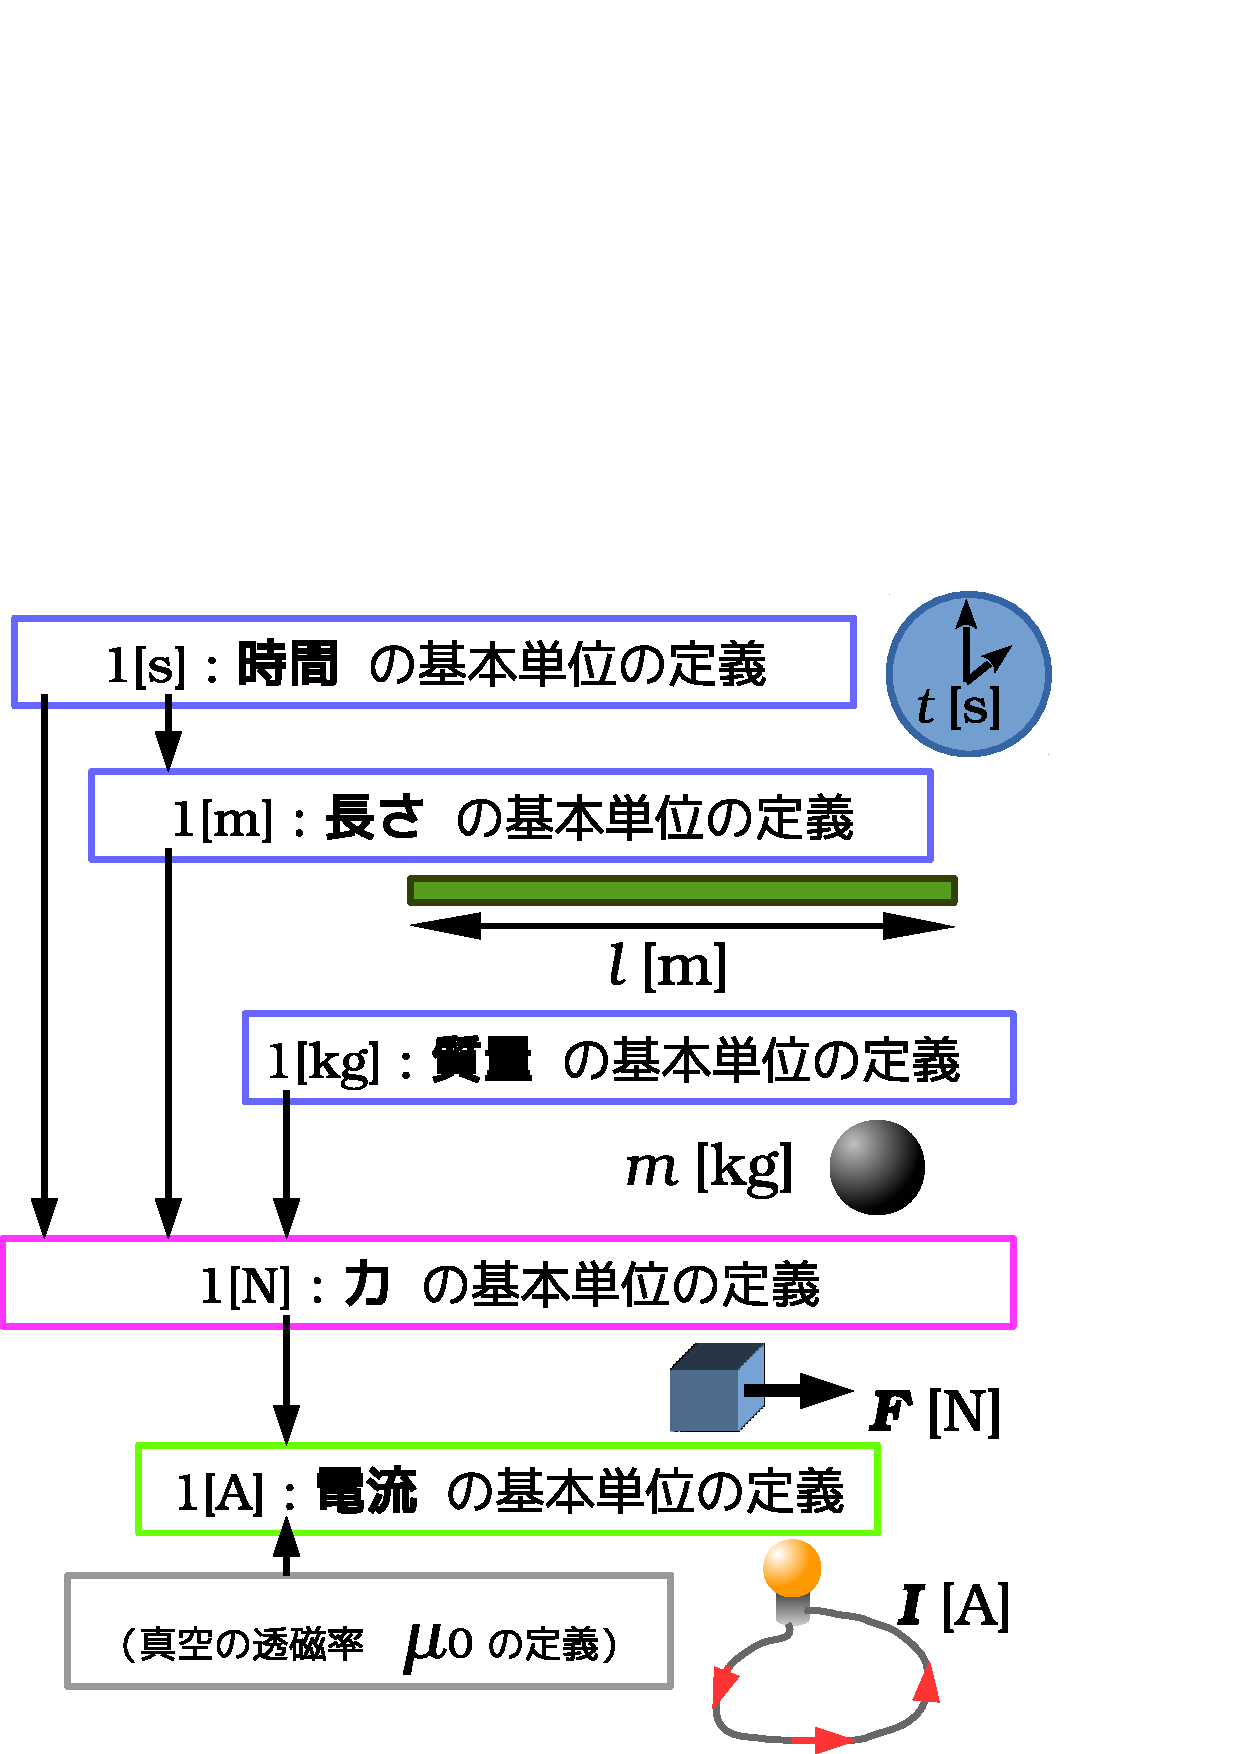
\includegraphics[keepaspectratio, width=7cm,height=8.42cm,clip]{tanni1.pdf}
                        \caption{単位の構成}
                        \label{fig:tanni1}
                    \end{center}
                \end{figure}

            最初に,原子の出す光の振動回数から,1[s]が定義される.
            そして,1[m]を光が1[s]で進む距離の1/$c$ ($c$ は光速の数値)と定義される.
            また,質量は,これらとは独立に,キログラム原器を基準に1[kg]が定義される.
            ちなみに,この1[s],1[m],1[kg]から力の単位[N](=[kg$\cdot$m/s${}^{2}$)が
            定義され,この1[N]を用いて,電流1[A]が定義される.電流の単位については
            電磁気学の項目を参照のこと.
            \end{memo}

%   %==========================================================================
%   %  Section
%   %==========================================================================
    \section{物理学における,数学の扱い方}
%       %======================================================================
%       %  SubSection
%       %======================================================================
        \subsection{道具としての数学}
            先に,物理学では数学を道具として扱うと説明した.道具として扱うとは,
            数学的厳密性を適宜無視して,数式を扱うということである.物理学の目的
            は自然現象を数式で表現することであり,重要なのは数式ではなく自然現象
            である.だから,物理学の教科書を読んでいて,数式が出てきた場合に,注
            意が必要なのである.

            数学を学習する上で大切なことのひとつに,厳密な証明の理解がある.だけ
            ど,数学を厳密に扱うとは,物理学ではあまり行わない.むしろ,厳密性を
            無視してしまっていることが多い
                \footnote{
                    例えば,テイラー(Sir Brook Taylor, 1685--1731, イギリス)展開
                    の高次の項は無視するということがある.
                }.

            物理学における数学は,あくまで道具なので,そんなに厳密に考える必要は
            ない.大切なのは,そのイメージできることである.研究者になるのでない
            限り,数学的厳密性に敏感になるよりも,数学を図形的にイメージできるよ
            うになることの方が大事である.言うまでもなく,私は研究者を目指してい
            るわけではないので,このノートでも数学的厳密性は全く気にしていない.
            このノートでは,数学を直感的に扱える程度で十分である.


%       %======================================================================
%       %  SubSection
%       %======================================================================
        \subsection{物理学の考え方}
            数学の命題や定義は絶対に不変である.後になって「間違いでした」なんて
            ことは起こらない.しかし,物理では間違いは起こる.そのたびに,修正が
            なされる.物理は実験や経験を基にしているからである.物理学ではある問
            題に対して,その原因をいろいろ仮説を立てて,実験的に仮説の正しさを確
            かめる.ここに人間の直感が介入してくる.この「人間の直感」こそが,数
            学と物理の大きな違いである.

            物理学は,感覚的なひらめきを基に構成される.だから,このひらめきが正
            しいかどうかを確認すべきだ.そのために,ひらめきを数式で表現
            して,実際に実験して検証する必要がある.物理学は,ひらめきとイメージ
            に重点が置かれているといってもよい.

            数学では考えられないことだろう.数学でも,問題を解くときにはひらめき
            はとても重要だ.そうなのだけど,物理学との違いはその検証の方法であ
            る.数学での検証は,数と論理のみで行う.そこには,実験や経験といった,
            人間の直感は含まれない.数学ではこの検証のことを「証明する」という.
            証明は数と論理で構成されいて,一度正しさが確認されれば
                \footnote{
                    (証明の)正しさの確認:論理に間違いがないことを確認すること.
                }
            後になって,間違いでしたということはない.数学に対して,物理学では,
            実験を行って,その検証を行う.実証するしかないのである.物理学では,
            証明はありえない.

            この実験が物理学の醍醐味なのだろう.自然を肌で感じ,数式で表現しさま
            ざまな予測を立てて,検証を行う.これが楽しいから,物理学があるのだ.


%       %======================================================================
%       %  SubSection
%       %======================================================================
        \subsection{物理学の数式の解釈}
            物理法則を表す数式において,等号は「\textbf{近似的に}等しい」という意味で使われる.

            数学における等号は,その右辺と左辺が全く同等であるという意味であ
            る,しかし物理では,例えば法則を数式で書き表すときに,右辺と左辺
            は本来は別々な概念であるのに,それらが等しいと書き表す.このよう
            なときに使われる等号は,“近似的”というような意味での等号である
            と考えるべきだ.この近似的という言葉も正確ではないが.なんという
            か,物理学独特の等号の使い方である.この原因は,物理学では,数学
            のような理論的厳密性よりも,\textbf{実験結果,経験が重要視される} と
            いうところにある.というのも,実験で得られる数値の桁は有限の桁で
            あり,それはもう既に近似である.だから,実験で得られる各法則も近
            似的であるし,物理の理論はこの近似の上で成立している.

            また,等号は定義するときに用いられることもある.

            もちろん,数学的な式変形のときの等号は,
            数学における等号の意味と同じである.
            これは,\textbf{恒等式} といわれる.

            \begin{memo}{恒等式}
                \textbf{恒等式} とは,変数 $x$ にどのような数を代入しても成立する
                式のことである.例えば,因数分解の公式
                    \begin{align}
                        {(x+y)}^{2}=x^{2} + 2xy + y^{2}
                    \end{align}
                がある.この式の $x$,$y$ にどのような数を代入しても,“恒に”成
                立する式である.
            \end{memo}

            \begin{memo}{方程式}
                式には,恒等式の他にも,\textbf{方程式} もある.方程式とは,例えば,
                変数 $x$ がある特別な数のときのみに成立する式のことである.その例
                として,以下の方程式を挙げよう.
                    \begin{align}
                        x^{2} - 2x + 1 = 0
                    \end{align}
                この式は,$x=1$ の場合のみにしか成立しない.このような特定の数値の
                みで成立する式が,方程式である.
            \end{memo}


%   %==========================================================================
%   %  Section
%   %==========================================================================
    \section{対称性 --- 物理学の基本要請 ---}
    \begin{mycomment}
        ここで,物理学の最も基礎となる考え方である,\textbf{対称性} について
        説明する.
        物理学には,その思想の基礎に,\textbf{対称性} という考え方を持っている.
        対称性とは,その名の通り,「どちらを見ても同じ」ということである.
        対称性という言葉は,実は,中学生の頃から使用している.
        例えば,点対称な図形は180${}^{\circ}$ 回転しても形を変えないという性質
        を持っている.また線対称な図形とは,左右あるいは上下で鏡を写したような
        形のことである.
        物理学で言う所の対称性は,点対称や線対称と同じような意味である.
        ただ違う点は,対象が図形ではなく,空間と時間に関する法則の性質である
        ことだけである.
        空間や時間の対称性とはとういうことかを,この節で説明していく.
    \end{mycomment}

%       %======================================================================
%       %  SubSection
%       %======================================================================
        \subsection{空間の対称性}
            \begin{mycomment}
                物理学では,暗黙のうちに,空間には縁がないと仮定されて理論が
                構築される.このノートでもこの原則にしたがう.具体的ないイメージ
                をしては,縁のない宇宙を想像すると良い.
                無限に広がる宇宙,あるいは,球の表面のように縁はないが有限の空間
                をイメージしてもらいたい.私達の存在するこの宇宙の具体的な形は
                不明であるが,以下の議論では,宇宙の具体的な形は問題とならない.
                将来,この宇宙の形は天文学的な観測によって明らかになることであろう.
                空間の対称性には2種類あり,次の通りである.
                    \begin{itemize}
                        \item 並進対称性
                        \item 回転対称性
                    \end{itemize}
                これらについて,以下で説明する.
            \end{mycomment}
%           %==================================================================
%           %  SubsubSection
%           %==================================================================
            \subsubsection{並進対称性}
                空間の並進対称性とは,どの方向に並行移動しようが,物理法則は
                全く変化しないということである.

                具体例で説明しよう.ある場所Aで実験していて,ある結果を得たとし
                よう.この実験結果は間違いがないものと,裏付けられたとする.こ
                の実験を別の場所Bで,全く同様の条件と方法で実験を行ったとき,
                実験結果はどうなるだろうか.全く同じ結果
                    \footnote{
                        実験誤差は当然考慮した上で.
                    }
                になるはずである.そうならなくては,その実験は正しいとは言えない.
                “どんな場所で,実験しても,実験条件と方法が同じであれば,同一の結果を得る”
                という考え方が,\textbf{空間の並進対称性} である.空間の並進対称性
                を信じているからこそ,正しい実験とその結果を受け入れることができるのである.
                ただし,並進対称性は,並進と言っているからには,実験している方向に
                関しては,していない.つまり,“同一の向きを向いて”という仮定が
                含まれているのである.

                もう一度言おう.空間の並進対称性は,場所Aで実験しても,
                場所Aから平行移動した場所Bでも,条件と方法が同じであれば,
                得られる結果も同じになるということを保証する.

                つまり,「どこで実験しても得られる結果は同じ」ということである.
                言い換えれば,\textbf{物理法則は場所により不変である}と言える.
                    \begin{myshadebox}{空間の並進対称性}
                        \textbf{空間の並進対称性} は,物理法則は場所によって不変であることを
                        主張するものである.
                    \end{myshadebox}

                    \begin{figure}[hbt]
                        \begin{center}
                            \includegraphics[keepaspectratio, width=7cm,height=3.23cm,clip]{Synmmetry_SpaceP.pdf}
                            \caption{研究所の並進移動}
                            \label{fig:Synmmetry_SpaceP}
                        \end{center}
                    \end{figure}


%           %==================================================================
%           %  SubsubSection
%           %==================================================================
            \subsubsection{回転対称性}
                並進対称性では,並進移動しても物理法則に何ら変化がないということが
                保証される.これに対して,回転対称性は,その名の通り,回転しても
                物理法則が変わらないことを保証している.ある向きで実験を行った
                とし,その後,同じ場所で別の向きで実験しても,向きを変える前と
                実験結果は同一になるということである.

                つまり,
                \textbf{空間の回転対称性} は,
                ある場所において,ある向きで実験する場合と,その場所で別の向きで
                実験する場合とで,同じ結果を得ることを保証する.

                つまり,「どの向きで実験しても,得られる結果は同じ」ということである.
                言い換えると,\textbf{物理法則は向きに対して不変である}と言える.
                    \begin{myshadebox}{空間の回転対称性}
                        \textbf{空間の回転対称性} は,物理法則が向きに対して不変である
                        ことを主張するものである.
                    \end{myshadebox}

                    \begin{figure}[hbt]
                        \begin{center}
                            \includegraphics[keepaspectratio, width=7cm,height=4.6cm,clip]{Synmmetry_SpaceR.pdf}
                            \caption{研究所の回転}
                            \label{fig:Synmmetry_SpaceR}
                        \end{center}
                    \end{figure}


%       %======================================================================
%       %  SubSection
%       %======================================================================
        \subsection{時間の対称性}
            時間の対称性が意味するところは,とても単純で,
            物理法則が時間に対して不変であることを主張するものである.
            要するに,いつ実験しようが実験結果は変わらないということ
                \footnote{
                    もちろん,条件,方法は同じである必要がある.
                }.
            朝に実験しようが,夜中に実験しようが,実験結果は全く同じ.
            朝の実験の方が良い結果を生むということは決して無い.
                    \begin{myshadebox}{時間対称性}
                        \textbf{時間の対称性} は,物理法則が時間に対して不変である
                        ことを主張するものである.
                    \end{myshadebox}
            
            \begin{memo}{「時間の対称性」への不信感}
                時間の対称性には,少し怪しいところがある.時間には「始まり」と「終わり」
                という概念があるためである.「始まり」や「終わり」の付近では対象性がなくなる.
                時間が「始まる前」と「始まった後」では対象性があるとは言いにくいだろう.
                ただ,「時間が始まる前」というイメージに具体的に説明することもできないので
                以降では,さしあたっては,時間には「『始まり』も『終わりも』ない」と割り切って,
                この問題を脇において考察をすすめる
                    \footnote{
                        「考えられないから,考えないように目をつむるしかない」というのが
                        本音である.
                    }.
                
            \end{memo}


%       %======================================================================
%       %  SubSection
%       %======================================================================
        \subsection{対称性 --- まとめ ---}
            \textbf{対称性} という専門用語を使うと,いかにも難しい概念だと思われる
            が,その意味はとても単純であり,私たちには暗黙の了解として体に染み付い
            ているものである.対称性のおかげで,研究所を建てる場合に,場所や向きや
            時代を考えることは必要がなくなる.いや,そもそも,物理法則は場所や向き,
            時間に対して不変でなければならないという要請がなされているものである,
            といった方が正確だ.

            つまり,物理法則というからには,対称性を備えていなければならない
            のである.物理法則は,場所にかかわらず,向きにかかわらず,時間(時代)
            にかかわらず,不変性を保つものである.
                    \begin{myshadebox}{対称性}
                        \textbf{対称性} は,物理法則に要請される性質の1つである.
                        物理法則は,場所や向き,時間にかかわらず不変でなければならない,
                        という要請である.対称性により,物理法則が不変であることを
                        保証するのである.
                    \end{myshadebox}


%       %======================================================================
%       %  SubSection
%       %======================================================================
        \subsection{対称性と保存則(ネーターの定理)}
            対称性からとても大切な性質が導かれる.詳細は,解析力学を
            学習するときに確認することだが,ここでは簡単に紹介しておこう.

            唐突で申し訳ないが,下表(\ref{tab:Synmmetry_and_Conservation})をみて
            欲しい.この表を見ながら,以下の説明を読んでもらうと,幾らかは
            わかりやすいと思う.
            \begin{table}[hbt]
                \label{tab:Synmmetry_and_Conservation}
                \caption{対称性と保存則の関係}
                \begin{center}
                    \begin{tabular}{l|l}
                        \multicolumn{1}{c|}{対称性} & \multicolumn{1}{c}{保存則} \\
                        \hline\hline
                        時間の対称性 & エネルギー保存の法則 \\
                        \hline
                        空間の並進対称性 & 運動量保存の法則 \\
                        \hline
                        空間の回転対称性 & 角運動量保存の法則 \\
                        \hline
                         ゲージ対称性 & 電荷保存の法則 \\
                    \end{tabular}
                \end{center}
            \end{table}

            物理学を学習していくと,場所や向きや時間に影響されない法則を
            見つけることができる.これは \textbf{保存則} と言われる.
            例えば,中学生の頃からおなじみの,力学的エネルギー保存の法則が
            ある.これも,保存則の1つである.更にこれを一般化して,
            単に,\textbf{エネルギー保存の法則} とされるが,このエネルギー保存則
            は時間の対称性から数学的に導かれるのである
                \footnote{
                    “導けてしまう”と言ったほうが,実際的かもしれない.
                    感覚は人それぞれだけども$\cdots$.
                }.
            つまり,数学の定理
            である \textbf{ネーターの定理}に時間の対称性を照らし合わせると,
            エネルギーがいつでも一定値をとる
                \footnote{
                    いつでも一定値をとることを,\textbf{保存する} という.
                    詳細は後述する.
                }
            ことが結論されるのである.

            同様に,空間の並進対称性からは,\textbf{運動量保存の法則} が得られる.
            また,空間の回転対称性からは,\textbf{角運動量保存の法則} が得られる.
            また,ゲージ対称性からは,\textbf{電荷保存の法則} が導かれる.
            ネーターの定理の具体的な意味と保存則に関する詳細は,後に改めて考えることとし,
            ここでは紹介程度にとどめる.



\chapter{運動学}
%   %-----------------------------------------------------------------------------------------------
%   %  Input
%   %    File Name : PhysNote_CM_Kinematics.tex
%   %    説明      : 物体の運動の表現方法について,記述する
%   %-----------------------------------------------------------------------------------------------
        %===================================================================================================
%  Chapter : 運動学
%  説明    : 物体の運動の表現方法について,記述する.
%===================================================================================================
%   %======================================================================
%   % Section
%   %======================================================================
    \section{「物体の運動」の表現方法}
    \begin{mycomment}
        物理学,特に力学の主な目的は,物体の運動軌道を(数学的に)推測する
        ことにある.これから学習する力学は,スペースシャトルを地球から宇宙へ飛ばす
        際に実際に使われる理論でもある.また,アメリカの人類初の月面着陸(1969)を実現
        するにも,この力学理論が使われている
            \footnote{
                もちろん,力学だけではない.スペースシャトルや宇宙服などに使われる装置
                を作る際に用いられる理論は,
                電磁気学,物性理論,電子回路論,材料工学など様々なものが使われている.
                しかし,スペースシャトルの打ち上げ方向を決めるのには,力学理論以外には,
                何も使用していない.摩擦や,宇宙での人間の行動を考えずに,単に宇宙に飛び出して
                月に行くことだけを考えれば,250年前にニュートンが創り上げた力学理論さえあれば
                よいのである.
            }.

       物体の運動を表すには,どのような概念があるとよいのかを,この節で説明していこう.
    \end{mycomment}
%       %======================================================================
%       %  SubSection
%       %======================================================================
        \subsection{位置}
        物理学の,ここでは特にニュートン力学の重要な目的の1つに,\textbf{物体の
        運動を記述する} ことがある.記述の仕方はどのようであってもよいが,最もよ
        く表現できる道具として,数式が有力である.実際に,物理学では物体の運動を
        数式を用いて表現している.数式で表現すれば,曖昧さ無しに,誰にでも全く同
        一のイメージを与えることができる.

        物体の運動は数式を用いて行うことはわかった.では,実際に数式で表現するに
        はどうすればよいだろうか.物体の運動を記述したいのであるから,まず“物体
        がどこに存在するかを示す指標”が必要になる.この指標のことを,\textbf{位置} と
        いう.物体はいつも同じ場所に存在しているとは限らない.時々刻々と,その位
        置を変化させている物体のほうが一般的である
            \footnote{
                少なくとも,地球上の物体(私たちの体を含めて)は,時々刻々とその
                位置を変化させている.なぜなら,地球は太陽に対して公転しているの
                であるから,地球の外側(宇宙)から見れば,地球上の物体はすべて動
                いているのである.
            }.

%       %======================================================================
%       %  SubSection
%       %======================================================================
        \subsection{速度}
        物体の位置が記述できれば,それだけで物体の運動を記述でるだろうか.否,
        明らかに不可能である.物体が“どのように”運動しているかということも,
        記述すべきだ.つまり,物体の \textbf{速度} も知っておかないと
        いけない情報の1つである.速度とは,単位時間あたりに,物体がどの程度
        移動したかを示す指標である.

%       %======================================================================
%       %  SubSection
%       %======================================================================
        \subsection{加速度}
        さらに言うと,物体の速度は常に一定であることは珍しく,速度も位置と同様に,
        時々刻々と変化している方が一般的である.この速度の時間変化のことを,
        \textbf{加速度} という.

            \begin{memo}{加加速度,躍度,jerk}
                「速度」,「加速度」とくれば,「加加速度」というものも
                考えられるのではないか.実際,その通りで,
                加加速度という概念は存在している.これは,「躍度(やくど)」と
                も言われる.英単語では,jerkがそれに相当する.
                加速度が急激に変化すると,機械におおきな負担がかかること
                になる.この負担を数値で示すのが,躍度である.

                ニュートンの運動の第2法則(運動方程式)で,加速度と力は比例関係にある
                ことが分かっているので,躍度とは力の時間変化であると言い換えることも
                できる.

                なお,ニュートン力学を学ぶにあたり,躍度という概念は
                使うことはない.
            \end{memo}


%       %======================================================================
%       %  SubSection
%       %======================================================================
        \subsection{運動軌道}
        物体が,ある位置で突然と消えてしまい,次の瞬間に全く別の場所から突然現れ
        ることはない
            \footnote{
                実は,このことは後で考える \textbf{エネルギー保存の法則} に関連
                したことである.
            }.
        つまり,言い方を変えれば,時間的に位置が変化する物体について,その位置を
        時刻ごとに記録していけば,物体の \textbf{軌道} を得られるということであ
        る.実はこの物体の軌道こそが,ニュートン力学で興味ある事なのである.物体
        の運動の記述をするということは,物体の運動軌道を記述するということなので
        ある.

        では,物体の軌道を記述するには,どうしたらよいだろうか.観測できるのは,
        物体の持つ今この瞬間の性質であり,一瞬にして運動軌道を得ることはできない.
        もちろん,時間をかけて観測すればその軌道は明らかになるが,この観測でわかる
        のは,観測の対象としている物体の軌道のみであり,一般の物体についてのもので
        はない.知りたいのは,「現在の物体のもつ運動状況」から物体の軌道を推測する
        方法である.

%       %======================================================================
%       %  SubSection
%       %======================================================================
        \subsection{「運動の軌道」の表現に必要な情報}
        物体の運動を記述するということは,物体の動く道筋である
        運動の軌跡を記述するということである.そして,物体の運動の軌跡を記述する
        には,物体の位置・速度・加速度の3つが必要である.さらに,物体の位置や速
        度は時間的に変化するものなので,当然,「時刻」も必要である.この4つの要
        素を基に,数式を用いた推論を行うことで,物体の軌道を表現できる.

        ここに挙げた4つの概念,つまり,時刻・位置・速度・加速度は,数式で扱う以上,
        何らかの文字で表す必要がある.そこで,これら4つに次のように文字を割当て
        ることにする.
        \begin{myshadebox}{運動の軌跡の表現に必要なもの}
            物体の運動を数式で表現するには,次の4つの要素が必要である.
            \begin{enumerate}
                \item 時刻:$t$
                \item 位置:$\br$
                \item 速度:$\bv$
                \item 加速度:$\ba$
            \end{enumerate}
        \end{myshadebox}

        なぜ時刻を表す $t$ は普通の太さなのに,他の3つの位置 $\br$,速度 $\bv$,
        加速度 $\ba$ は太文字で表現されるかという,疑問があることと思う.これに
        ついては,この後に説明する.ここでは,このような文字が割当てられている
        ということを,知ることができれば十分である.

        ちなみに,このようなアルファベット($t$,$\br$,$\bv$,$\ba$)を割
        当てる強い理由はない.大切なのは,文字に意味を割当てるということであり,
        文字が何を意味するかではない.どのような文字を割当てても,全く同じよう
        に議論できることは明白である.ここでは,単に慣習に従って
            \footnote{
                私は単に多くの教科書で採用されている記号を流用しているに過ぎない.
                偉そうなことを書いたが,教科書でなぜこのように文字を割当ててい
                るのかは分かっていない.
            },
        時刻 $t$/位置 $\br$/速度 $\bv$/加速度 $\ba$ と割当てただけである.
        英単語を見てみると,
        時間はtime,点(位置)はrespect,速度はvelocity,加速度はacceleration
        である.その頭文字をとっているのかもしれない.

%   %==========================================================================
%   %  Section
%   %==========================================================================
    \section{位置の記述方法}
        \begin{mycomment}
            物体の存在する位置(場所)を表現することを考えてみよう.
            例えば,物体が「ここにある」とか「あそこにある」
            といっても,見る人によって見える方向は違ってくる.
            例えば,二人の人間の真中に静止している
            ボールがあるとして,そのボールは一方の人から見れば
            「右側」にあるというだろうし,
            もう一人は「左側」にあるというだろう.この場合,
            ボールが静止しているのにもかかわらず,
            二人のボールの位置に関する主張は異なっている.
            これではどうにもこうにも話が進まない.
            ここでは,この問題を解決することを考える.
        \end{mycomment}


%       %======================================================================
%       %  SubSection
%       %======================================================================
        \subsection{1次元(直線)上の位置}
                まず,最も簡単な直線上の位置を表すことを考えてみよう.
                その方法とは,
                直線の各点に数字を貼り付けて,その数字によって位置を表すというものである.
                図\ref{fig:ichi1}参照.
                このように直線上で表される位置を,\textbf{1次元} という.
                \begin{figure}[hbt]
                    \begin{center}
                        \includegraphicsdefault{ichi_1jigen.pdf}
                        \caption{1次元(直線上)での位置}
                        \label{fig:ichi1}
                    \end{center}
                \end{figure}

                位置を指定したいときは,まず,「基準」とする位置を決める必要がある.
                この基準の位置は直線上であればどこでもよいが,一度基準の位置を決めたら絶対にこの基準を
                変更してはいけない.基準はOと表記される.
                この基準から左右の直線に,数字を貼り付けていく.
                そして,直線上の物体の位置をその実数で表すのである.ここで大切なことは,
                \textbf{位置と実数が1対1に対応している} ことである
                        \footnote{
                        “1対1に対応している”ということは,『
                        位置を1つ指定したならば,それに対応する実数が1つだけに決まり,
                        逆に数字を1つ指定したならば,それに対応する位置が1つだけに定まる』ということである.
                        }.
                図\ref{fig:ichi1}で,
                点Bの位置を示すときには,$-2$といえばよい.同様に,点Aを示すには$-6$を,点Dを
                示すには$3.9$をいえばよい.つまり,「点の位置は$-2$である」とか,「点の位置は3.9である」
                とかといって,位置を表現するのである.数式的に書けば,例えば点Bの位置が$-2$であるならば
                    \begin{equation*}
                        \mbox{点{\rm B}の位置} = -2
                    \end{equation*}
                のように書けるだろう.“点の位置”という日本語ではこれから式を扱っていく上で
                不都合があるから,これを記号で表現しようと思う.すなわち
                位置を表す記号を導入し,これを $r$ と書くことにするということだ.
                すると上の「点Bの位置$=-2$」は
                    \begin{equation*}
                        r= -2
                    \end{equation*}
                のように表現できる.しかし,
                点があるのは$-2$という位置だけとは限らず,どのような場所にも
                存在する.そこで,この$-2$とか3.9とかという具体的な位置を
                表現する記号が必要となる.そこで,
                位置の代表を文字 $x$ で表現する.すると,
                \begin{align}\label{eq:rx}
                r=x
                \end{align}
                というように位置を指定できる.$r$ は単に位置を表現する記号であって,
                $x$ はその位置の“任意のどこか”を示している.$x$ には何か特定の実数を入れる余地がある.
                例えば $r=5$ と書いたならば,実数が5という位置を指定したことになる.$r=8.15$ と書いたならば,
                実数が8.15と書かれた位置を指定したことになる.このように,$x$ は何らかの数を代表していて,
                様々な実数を入れることができる.$x$ に入れる実数をいろいろ変えることができると考えて,
                $x$ のことを \textbf{変数} という.

                位置を表す実数の絶対値 $|x|$ は原点 O からの \textbf{距離} を表現
                している.このように考えれば,位置の単位として $\mathrm{[m]}$ が用いられるのも
                納得がいくだろう.
                以上が1次元(直線)上における位置の表現の仕方である.

%       %======================================================================
%       %  SubSection
%       %======================================================================
        \subsection{2次元(平面)上の位置}
                次に,平面上(2次元)の位置の表現方法を考える.位置を考えるには2つの数字を用いる必要がある.
                1次元のときは1方向だけを考えればよかったが,2次元の時には,
                2方向($x$ 方向と $y$ 方向)について考えられるからである.図\ref{fig:ichi2}参照.
                \begin{figure}[hbt]
                        \begin{center}
                        \includegraphicsdefault{ichi_2jigen.pdf}
                        \caption{2次元(平面上)での位置(2次元直交座標)}
                        \label{fig:ichi2}
                    \end{center}
                \end{figure}

                $x$ 方向と $y$ 方向の軸が直交しているので,\textbf{2次元直交座標} とよばれる.
                2次元上での位置を表現したい時には,
                数字を2つ指定する必要がある.この2つの数の代表は $x,\,y$ で表されることが多い
                \footnote{
                    その他の表現として,$x_{1},\,x_{2}$ というように書かれることもある.
                    これは数の個数が多くなった時に有効な表現である.しかしここでは,馴染みの深い $x,\,y$ で
                    書くことにしている.
                }.
                例えば,図\ref{fig:ichi2}で点Aの位置を
                示したいときは,
                \begin{align*}
                x=3\,,\,\,y=2
                \end{align*}
                と表現されるが,これでは少し見づらい.そこでここでも,
                位置を表現する記号として,$\br$ を用いる.
                ここで $r$ のように細い文字で書かないで,$\br$ のように
                太字で書いたのは,複数の数の組であることを強調したいからである.
                具体的な数の組は $(x,\,y)$ と表現され,すなわち,図\ref{fig:ichi2}の紫色の点の位置は
                \begin{align}
                \br=(3,\,2)
                \end{align}
                のように書かれる.これは,$x$ 方向が 3 という数字のところで,かつ,
                $y$ 方向が 2 という数字であるような位置を指定していることになる.
                一般には,
                \begin{align}
                \br=(x,\,y)
                \end{align}
                というように表現される.2つの変数を使って,
                任意の平面上の位置を表現するのである.

                また,図形的なイメージとして“矢印”が導入される.
                この矢印の始点は必ず原点 O にとるとし,終点は
                指定したい点にとる.
                自分が原点 O に立って,指定したい点を指で差していると考えればよい.
                この矢印のことを \textbf{ベクトル} という.もっと一般的にいえば,
                座標のように複数の数の組で表現されるものをベクトルという.
                平面上のベクトルは2つの数で表現でき,これを2次元ベクトルという.
                一般に,$n$ 個の数で表現されるベクトルを \textbf{$n$ 次元ベクトル} という.

                1つのベクトルは \textbf{向き} と \textbf{大きさ} をもつ.原点を始点にもつベクトルの向きは,
                終点の座標によって表される.例えば,原点 O を始点として,点 ($x_{1}$,\,$y_{1}$) を終点
                とするベクトル $\br$ のむきは,($x_{1}$,\,$y_{1}$) といえばよい.
                「北に何歩,東に何歩」というイメージをすればよい.
                また,ベクトルの大きさ $r$ は
                    \footnote{
                        一般にあるベクトル $\ba$ の大きさを表現したい場合は,細字にして $a$ と
                        表現されることが多い.つまり,$a:=\|\ba\|$ である.
                    }
                ,三平方の定理によって,以下のように定義される
                \begin{align}
                    r: = \|\br\| =\sqrt{{x_{1}}^{2}+{y_{1}}^{2}}.
                \end{align}
                \begin{figure}[hbt]
                        \begin{center}
                        \includegraphicslarge{vector_learge.pdf}
                        \caption{ベクトルの大きさ(2次元)}
                        \label{fig:vector_learge}
                    \end{center}
                \end{figure}

                もちろん上記は,($x_{1}$,\,$y_{1}$) に限らず,任意の点 ($x$,\,$y$) で成立するので,
                以降では,($x$,\,$y$) と書くことにしよう.
                ベクトルの向きのみを示したい場合は ($x$,\,$y$) と示す以外に, ($x/2$,\,$y/2$)とか,
                (1,\,$y/x$) とかといった表現方法も可能である.しかし,向きを指定するのにこのような方法を
                とってある記述を見たことがない.
                具体的な位置 ($x$,\,$y$) が指定されれば,この座標から大きさ $\sqrt{x^{2}+y^{2}}$ が
                計算でき,さらに向きも指定できるということから,この座標表現によって,ベクトルが記述される.
                しかし,この表現は少し長ったらしくなったり,式に複数のベクトルがあったりすると見づらくなって
                しまうので,$\br$ というような太字でベクトルを表すことが多い.


%       %======================================================================
%       %  SubSection
%       %======================================================================
        \subsection{3次元(空間)内の位置}
            ここまで説明すれば,
            3次元(空間)内の点の位置の表現の仕方は明らかだろう.
            空間には平面の場合に加えて,“高さ”があると考えられる.
            この“高さ”に対する変数を $z$ と表現する.
            そうすると,空間内の位置を表現するには $x,\,y,\,z$ の3つの変数が必要になることが
            わかる.2次元上の位置を表現するのに $\br$ という記号を
            導入したが,3次元空間以上の次元でもこの記号 $\br$ を
            使用しする.
            3次元空間内の点の位置を表現するには
            \begin{align}
            \br=(x,\,y,\,z)
            \end{align}
            と表現される.$x$ 方向と $y$ 方向と $z$ 方向の3
            つの軸が直交しているので,\textbf{3次元直交座標} という.
            これ以降,位置を考えるときは3次元空間内の位置であるとする.

            「座標を決める」ということは「$\left( x, y, z \right)$ の3つの実数の組を決める」ということである.
            この式の意味するところは,\textbf{位置と座標が1対1で対応している} ということである.
            すなわち,座標が決定されると位置が確定される.
            逆に位置が決定されると,座標が決まる
                    \footnote{ここで1つ注意しておく.
                    位置が $\br$ が $\left( x  , y ,  z \right)$ の
                    組み合わせを決めることでその位置を指定できるからといって,
                    位置 $\br$ が $\left( x  , y ,  z \right)$ の
                    関数であると考えてはいけない.なぜなら,「位置を決めること」
                    と $\left( x  , y ,  z \right)$ の組み合わせを決めることは,
                    全く同じことであるからである.} .
            \begin{figure}[hbt]
                \begin{center}
                    \includegraphicslarge{ichi_3jigen.pdf}
                    \caption{3次元直交座標}
                    \label{fig:zahyou}
                \end{center}
            \end{figure}

            一般に,点の位置 は各時刻によって異なる.しかし時刻を指定すると,1つの決まった位置を示す.
            従って,位置 は時刻の関数である.
            これを,$\textit{\textbf{r}\rm{(}$t$\rm{)}}$ と書く.
            すなわち,時刻 $t$ のときの座標を $x(t), y(t), z(t)$ と表すと,
                \begin{align}
                        \br(t) = \left( x(t), y(t), z(t) \right)
                \end{align}
            の関係を表せる.
            全ての時刻で点の位置を記録すれば,
            その点は曲線を描く.これを物体の \textbf{軌道} という.

            また,位置の図形的なイメージとして,3次元の場合も“矢印”が導入される.
            この矢印の始点は必ず原点 O にとるとし,終点は
            指定したい点にとる.
            自分が原点 O に立って,指定したい点を指で差していると考えればよいと思う.
            空間内の位置は3つの数で表現できるから,
            空間内の位置は3次元ベクトルである.

            \begin{memo}{次元とは何か}
                物理学的に考えて,線上の位置は1つの数値で表せる.
                また,面上の位置は順序付けされた二つの数値を用いて表現する
                \footnote{
                    「順序付けされた」という言い方は,次のようなことを意味する.
                        \begin{equation*}
                            \left[\, a ,\, b \, \right] \neq \left[\, b, \,a \, \right].
                        \end{equation*}
                    つまり,ベクトル $\left[\, a ,\, b \, \right]$ の成分 $a$,$b$ には
                    順番があって,この順番を入れ替えてしまうと,全く別のベクトルになって
                    しまうということである.これは $a$ と $b$ の記述順序にも意味が含まれ
                    ていることを説明してくれる.数学では,このような数の組みのことを,
                    \textbf{順序対} という言葉で表現される.ベクトルは順序対のひとつの例
                    であると考えることができよう.
                }.
                この考え方は空間内の点の表現にまで同じように拡張されて,空間
                内の点は順序付された三つの数値で表される.

                しかし,だからと言って,面上の点の位置を示すのに,絶対に二つの
                数が必要かと問われれば,必ずしもそうとは限らない.
                例えば,面を適当な大きさの区画に区切り,そのうちの任意の一箇所を原点とし
                て0という数値を割当ててみる.そして,その周りを囲む区画に対して,
                順に自然数を割当ててみよう(図\ref{fig:JigenTohaNanika_MATH}).
                こうすれば,面上の任意の区画を1つの自然数で表せる.
                この区画を無限に小さくしていくと,面上の一点を1つの数値に対応させる
                ことができそうな気がする.
                \begin{figure}[hbt]
                    \begin{center}
                        \includegraphicsdefault{JigenTohaNanika_MATH.pdf}
                        \caption{次元とは何か}
                        \label{fig:JigenTohaNanika_MATH}
                    \end{center}
                \end{figure}

                もちろん,こんなに簡単に上手くいくはずはない.だけど,ただ漠然と考
                えていただけでは,面上の点の位置を表現するには
                は二つの数値が絶対必要だと,思い込んでしまいがちである.
                「本当にそうだろうか」と常に疑いの精神を持ちながら,
                教科書を読み進めることも大切な事である
                    \footnote{
                        場合によっては,鵜呑みすることが理解への近道であることもあるが,
                        そんな場合でも,あとで確認することを怠ってはいけない.というか,
                        いつの間にかその鵜呑みが体に染み付いて,当たり前のように感じるよ
                        うになってしまい,確認することを忘れてしまってはいけない.
                    }.
            \end{memo}

            \begin{memo}{座標の張り方}
                座標を張ると言っても,いろいろな張り方がある.なので,
                同じ物体の位置を表現するにしても,その座標の張り方によって,
                その位置を示すベクトルも異なってくる
                    \footnote{
                        原点Oからみた物体の位置を示す矢印が変わってくるということ.
                    }.
                具体例を描くと,図\ref{fig:ZahyouChokkouChokusen}(A,B,C,D)の
                ようである.

                もちろん,この4つの例以外に限ったことではなく,あくまで一例である.

                図\ref{fig:ZahyouChokkouChokusen}(A)を基準に話すと,
                (B)は座標の間隔を大きめにとっているし,(C)は斜めにとっていて,
                (D)は(C)と同様だが原点の位置を変えている.

                要するに,座標の張り方は無数に存在するということである.
                だから,二人の観測者が同じ物体を見ていたとしても,座標の
                張り方が異なっていれば,当然ながら,物体の位置を表すベクトル
                が異なる.これは,一見してみると,大問題に見えるかもしれない.
                座標の張り方によって物体の位置が変わってしまうからである.
                しかし,これは別に大した問題ではないのだ.むしろ,
                この方が好都合なのである.大事なのは,“観測者に対する物体の位置”だ
                からである.いいかえれば,万人に共通の物体の位置
                    \footnote{
                        この考え方は,後に説明する \textbf{絶対空間} に関連する
                        ものである.ニュートン力学は,この絶対空間の存在は,
                        暗黙の内に前提とされている.
                    }
                を示す必要はない,ということである.知りたいのは,それぞれの観測者
                からみた物体の位置であり,すべての観測者から見た物体の位置ではない.
                そもそも,すべての観測者は同じ位置に立つことはありえないから
                    \footnote{
                        同じ場所に二人の人間が立てるはずがない.
                    },
                観測者が個々に,自身のいる場所が原点となるように座標を取ることで,
                補正が必要なくなり,計算が楽になるのだ
                    \footnote{
                        自分の位置を原点にとることで,自身の場所を意識することなく計算
                        ができるようになる.もし,万人に共通な座標を取らないとならない
                        ならば,自分のいる位置を把握し,物体と自分の相対的な位置関係も
                        考慮して計算をしないといけなくなる.
                    }.
                \begin{figure}[hbt]
                                        \centering
                    \begin{tabular}{cc}
                        \begin{minipage}{0.45\hsize}
                            \begin{center}
                                \includegraphicsdouble{ZahyouChokkouChokusen001.pdf}

                                (A)
                            \end{center}
                        \end{minipage}
                        \begin{minipage}{0.45\hsize}
                            \begin{center}
                                \includegraphicsdouble{ZahyouChokkouChokusen002.pdf}

                                (B)
                            \end{center}
                        \end{minipage}
                    \end{tabular}
                \end{figure}
                \begin{figure}[hbt]
                                        \centering
                    \begin{tabular}{cc}
                        \begin{minipage}{0.45\hsize}
                            \begin{center}
                                \includegraphicsdouble{ZahyouChokkouChokusen003.pdf}

                                (C)
                            \end{center}
                        \end{minipage}
                        \begin{minipage}{0.45\hsize}
                            \begin{center}
                                \includegraphicsdouble{ZahyouChokkouChokusen004.pdf}

                                (D)
                            \end{center}
                        \end{minipage}
                    \end{tabular}
                                \caption{座標の張り方}
                                \label{fig:ZahyouChokkouChokusen}
                \end{figure}

                しかし,いいことばかりではない.二人の観測者間で,同じ物体の位置
                が異なるため,互いに相手の目線に立ちたい場合には,位置ベクトルに
                変換を施さないといけない.
                といっても,難しい変換をするのではなく,単に,
                自分から見た相手の位置 $\bV$ を,相手から見た物体の位置 $\bU$ に
                加えてやらないといけないということ.すると,$\bW(=\bV+\bU)$ により,
                他の観測者からみた物体の位置を把握できるようになる(図\ref{fig:SoutaiTekiIchi001}).

                まとめておこう.座標の張り方は様々であり,どう取るかは,観測者
                自身が自由に選べる.これにより,観測者は計算が楽になるように
                座標を設定できる.しかし,その欠点として,複数の観測者
                間で,物体の位置が異なっていしまう.この欠点は,座標の変換という
                手段で解決する必要がある.
                    \begin{figure}[hbt]
                        \begin{center}
                            \includegraphicsdefault{SoutaiTekiIchi001.pdf}
                            \caption{相対的な位置の関係}
                            \label{fig:SoutaiTekiIchi001}
                        \end{center}
                    \end{figure}
                \end{memo}


%   %==========================================================================
%   %  Section
%   %==========================================================================
    \section{速度・速さの表現方法}\label{subsec:Velocity}
%       %======================================================================
%       %  SubSection
%       %======================================================================
        \subsection{「速度・速さ」の表現方法}
            速さとは何か.当たり前すぎて,問うまでもないかもしれない.だけど,
            これを定量的に(数学的に)扱うために,速さという感覚を整理しておきたい.

            世の中には,いろいろな速さがある.例えば,
            人間の歩く速さ,自転車の速さ,自動車の速さ,電車の速さ,新幹線の速さ,飛行機の速さ.
            これらは,順をおっていくほど速さが増すことは,誰でも承知している.
            日常生活ではこのくらいの感覚で支障はないが,数学的に扱うには,このままでは不十分だ
                \footnote{
                    速さという概念を,こんな適当な感じだけで捉えて,自動車の
                    速度制御装置を作られているはずがない.速さを定量的に扱い
                    計算できるようにすることで,初めて速さを制御できるようになる.
                }.
            物理学は速度を数学的に扱うために,計測できる量を基に,速度
                \footnote{
                    さっきまで,「速さ」と言っていたところを,「速度」と
                    言い換えてしまった.以降では,語彙「速さ」,「速度」は
                    物理学の専門用語として扱うことにする.物理学では,
                    この2つの語彙は,それぞれ異なる意味が与えられている.
                    その違いはこの節の最後に記述した.
                }
            を定義する.速度を定義するのに必要な量は,位置と時間である.
            もっと詳しく言うと,“位置の変化量”と“位置の変化に必要とした時間”である.
            これらを用いて,速度は言葉を用いて書くと次のように定義される.
                \begin{align}
                    \mbox{速度} := \frac{\mbox{位置の変化量}}
                                       {\mbox{位置の変化に必要とした時間}}
                \end{align}

            やはり,言葉で書いたのでは見難いし,数式的に扱うこともできない
                \footnote{
                    できなくはないが,非常に面倒くさい.記述も煩雑になり,
                    読みづらい.
                }.
            なので,上の速度の定義を,文字による表現に書き換えないといけない.
            物体の運動方向は3つ(3次元)だけど,最初から3方向の速度を定義する
            には,おそらく,難しいことだろう.そこで,段階を分けて,1方向/2方向/3方向 と
            順に考えることにしよう.

            話が長くなるので,ここで一度,節を区切ろう.

        \begin{memo}{「速度」と「速さ」の使い分け}
            日常生活において,私たちは「速度」と「速さ」という2つの語彙を意識して使
            い分けることはしていない
                \footnote{
                    少なくとも,私は使い分けていない.
                }.
            しかし,物理学において,「速度」と「速さ」という言葉は意味のことのなるも
            のとして,下のように区別して使用される.
                \begin{itemize}
                    \item \textbf{速度} とは,向きを含む,ベクトルである
                    \item \textbf{速さ} とは,向きを含まない,スカラーである
                \end{itemize}

            口頭で話すときには,両者を意識せずに混同てしまいがちだが,
            大抵の場合,話の流れからどちらを意味しているかを判断できる.
            しかし,文書に著す場合には,両者を区別して記述したい.
        \end{memo}

%       %======================================================================
%       %  SubSection
%       %======================================================================
        \subsection{「変化」の数式化}
        \begin{mycomment}
            速度とは,位置の時間的な変化で表せることが分かった.
            では,変化をどのように表現すべきか.
            変化を定量的に扱えるようにするため,数式による変化の扱い方を学習する.
        \end{mycomment}
        物理学で主に行われることは,物体の構造解析と,物体の運動規則の探究である.
        物体の構造解析で今までに分かっていることは,いま私たちが目にしている物体
        は,すべて素粒子で構成されているということだ
            \footnote{
                素粒子とは何かとか,それがどうのように構成されているのか等の
                疑問は,このノート全体を通して探っていくことである.
            }.
        しかし,しばらくの間は,物体の構造ではなく,運動規則を考えていこう.
        物体の構造を解析するためには,物体の運動規則を知っている必要があるからだ
            \footnote{
                生の原子や分子は顕微鏡ですら見ることはできない.運動規則から
                推察し想像するしかないのだ.
            }.

         運動規則を定量化するには,変化を数式で表現する必要がある.
         物体の運動を調べるというとは,物体の動く軌跡を把握するということであり,
         その軌跡は物体の位置が変化することによって描かれるからだ.
                    \begin{figure}[hbt]
                        \begin{center}
                            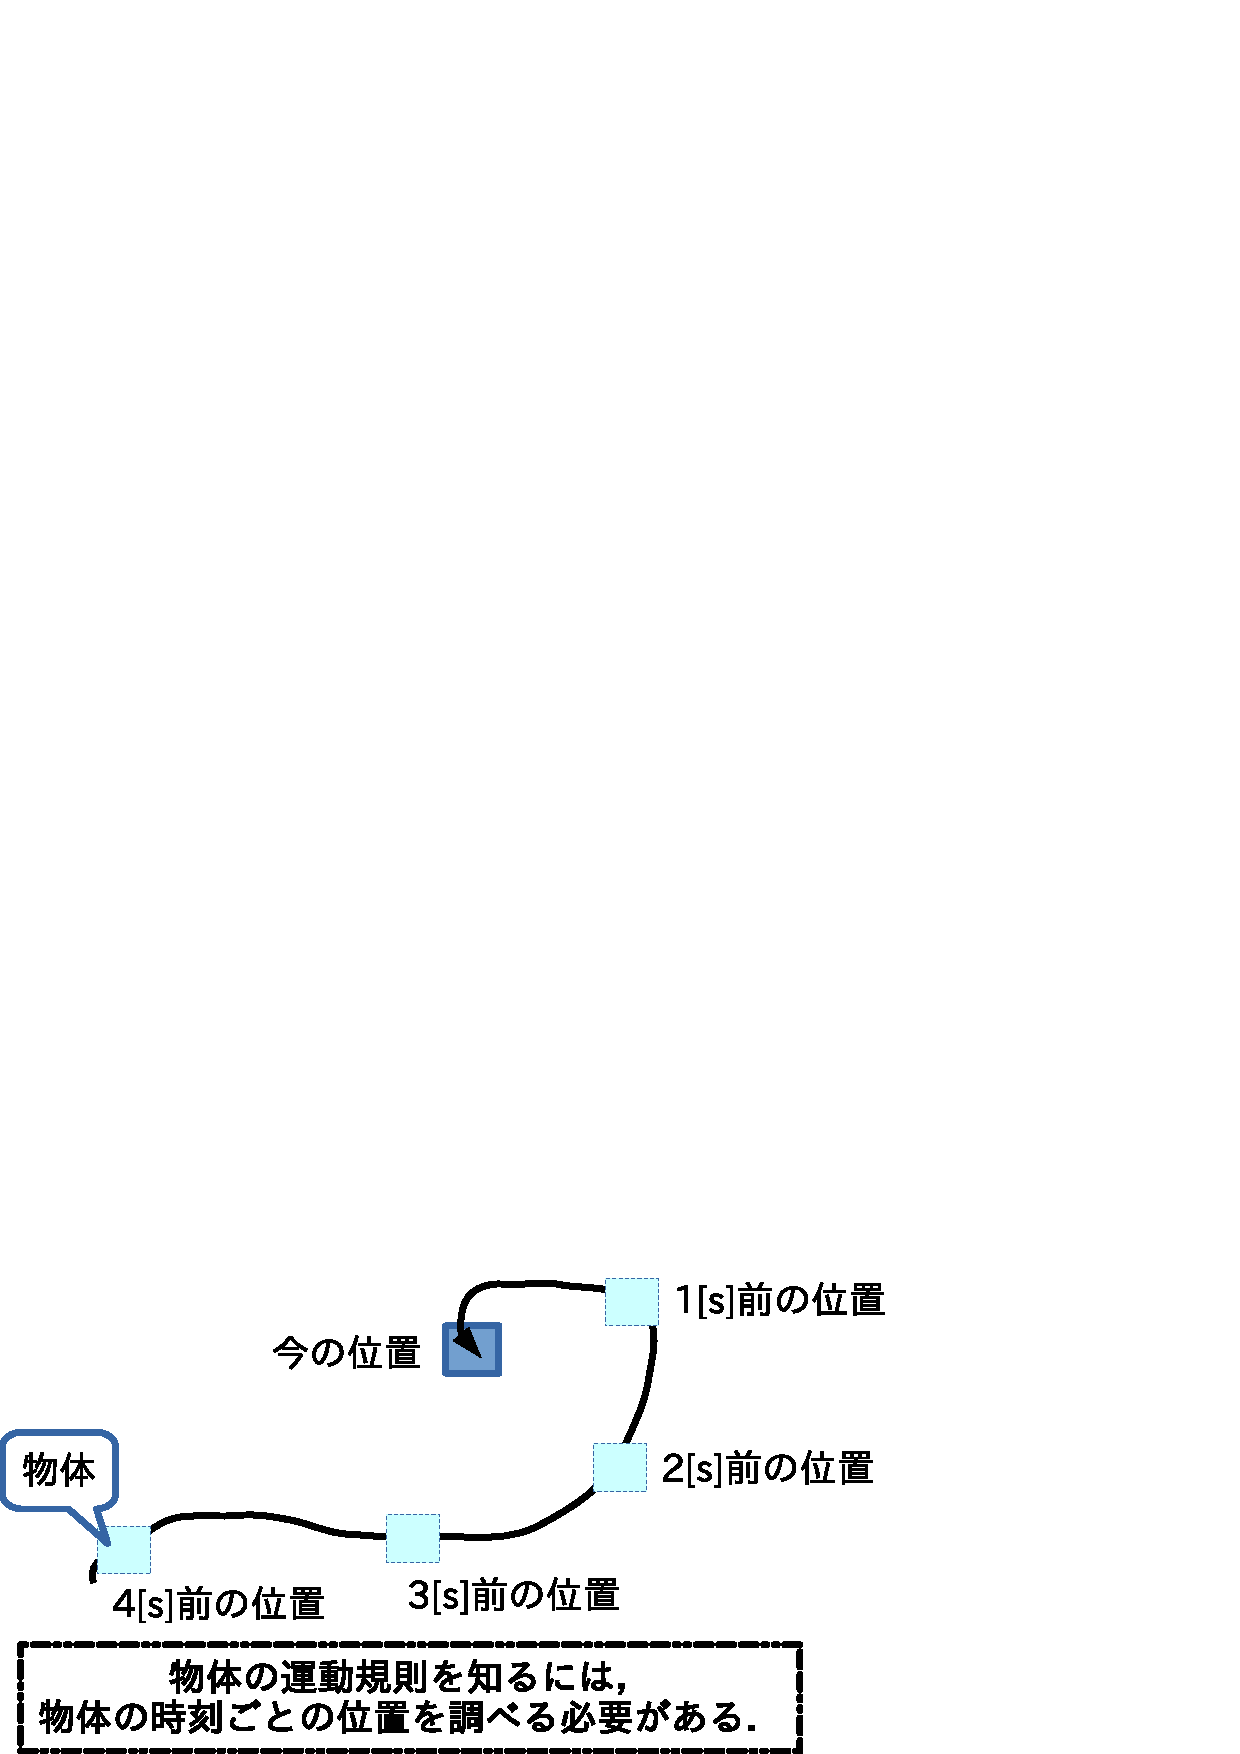
\includegraphics[keepaspectratio, width=7.2cm,height=3.72cm,clip]{henka0001.pdf}
                            \caption{軌跡$=$時刻ごとの位置の記録}
                            \label{fig:henka0001}
                        \end{center}
                    \end{figure}

%       %======================================================================
%       %  SubSection
%       %======================================================================
        \subsection{位置の時間変化の図示}
        物体の位置の時間変化を1つの図で表現する場合,
        次のように書ける.

        最初の位置を $\br_{1}$ として,次の位置 $\br_{2}$ に移動したという場面を考える.
        $\br_{1}$ から $\br_{2}$ に変化したのであるから,位置の変化分 $\br$ は
        \[
            \br = \br_{2} - \br_{1}
        \]
        とかける.
        \begin{figure}[hbt]
            \begin{center}
                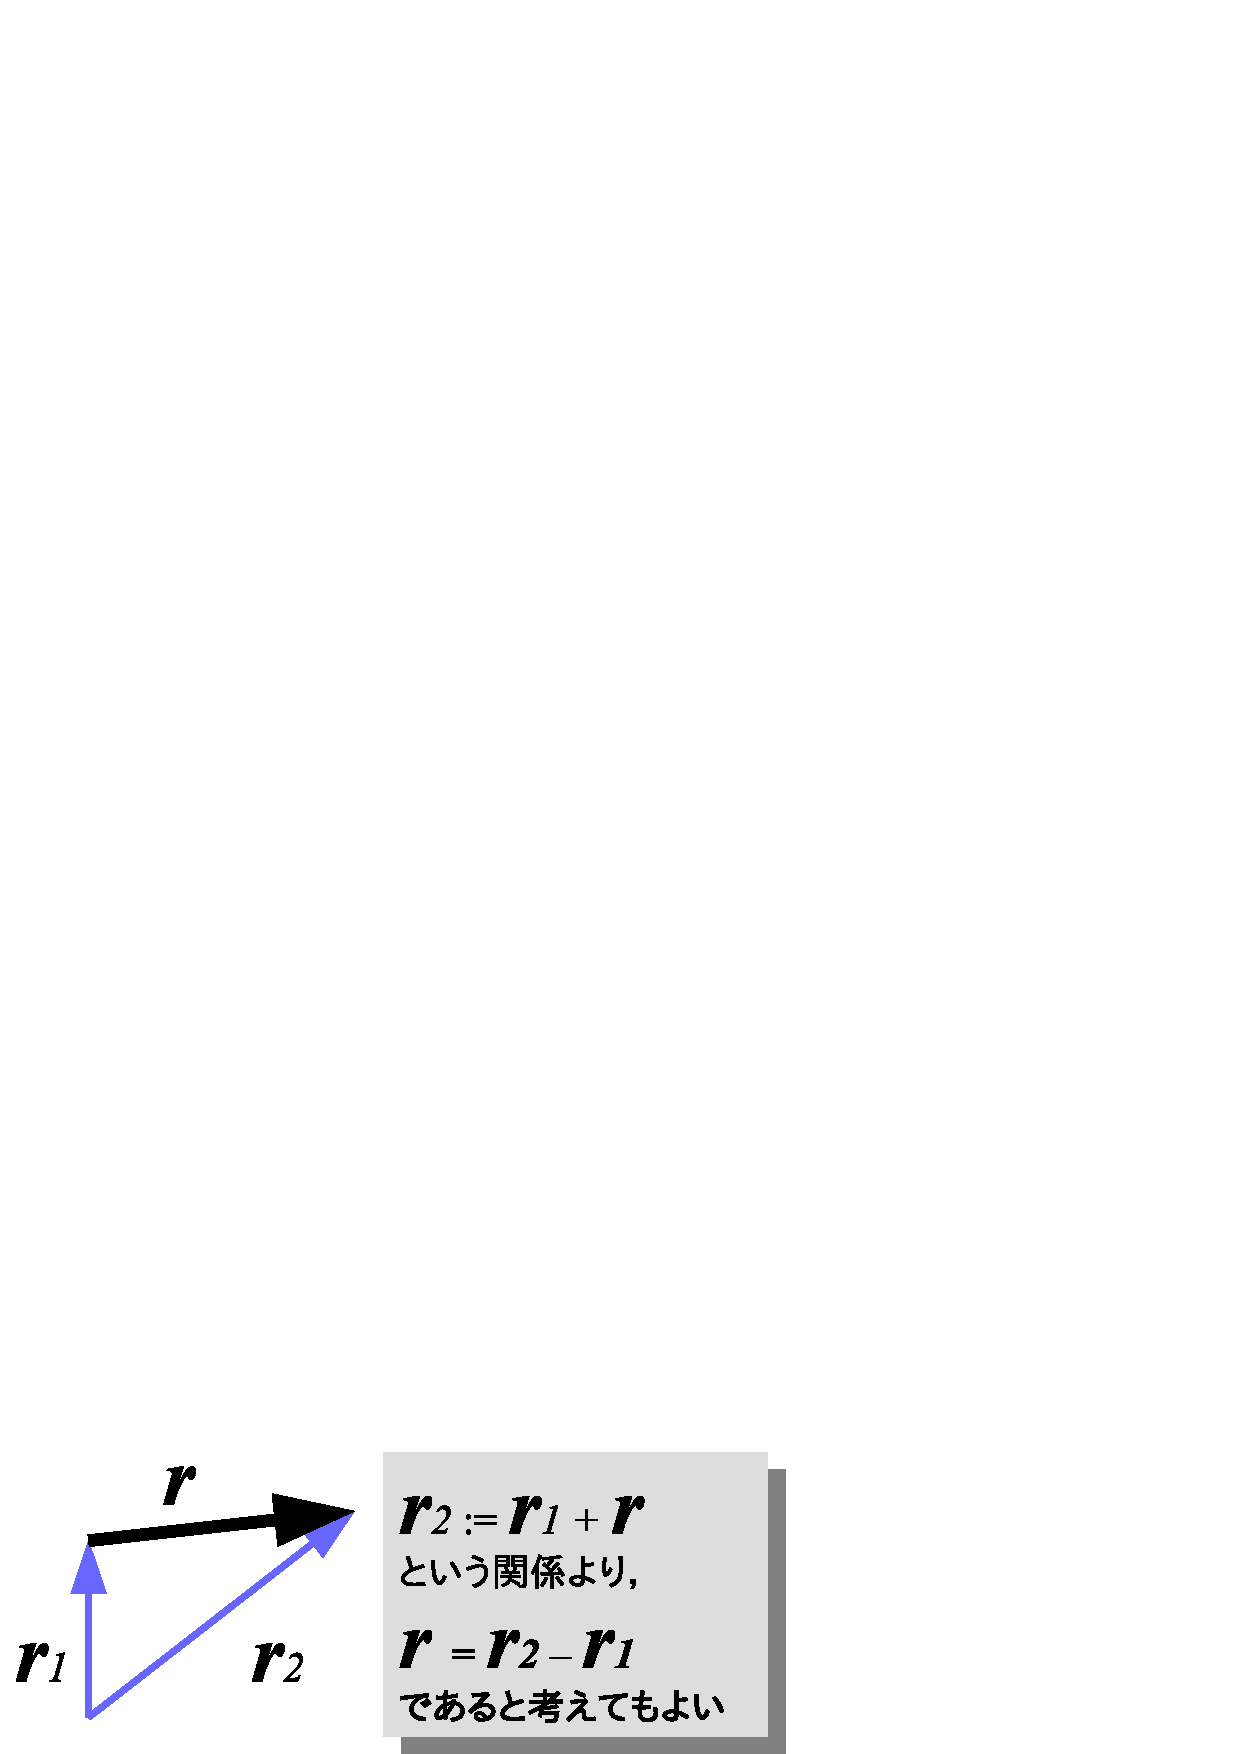
\includegraphics[keepaspectratio, width=6.2cm,height=3.2cm,clip]{ichi_henka.pdf}
                \caption{ベクトルの引き算}
                \label{fig:ichi_henka}
                \end{center}
        \end{figure}


%       %======================================================================
%       %  SubSection
%       %======================================================================
        \subsection{1次元(直線)上の速度}
                最初に,直線上を動く物体の様子について考えてみる.
                物体が直線上を運動するとき,物体は様々な速さで動くだろう.
                また,物体は直線上を右から左へ,もしくは左から右へ気まぐれに
                動くだろう.このような物体の運動を記述するにはどうすればよい
                だろうか.

                物体は直線上を動くと仮定しているので,物体は必ず直線上に存在し,$x(t)$ とい
                う1つの数で表現できる.
                物体が“動く”ということは, \textbf{時刻変化に伴って位置を変える} というこ
                とである.従って,
                時刻の変化 と 位置の変化 を考えれば物体の速さを表現できると考えられる.では,
                時刻の変化と位置の変化
                をどのように用いれば,速度を表現できるだろうか.その解決方法は,
                時刻の変化に対してどの程度の位置が変化するかという
                ことを表現すればよい.具体的に,2秒間で5[m]進む時の速さ と,
                3秒間で8[m]を進むときの速さ を考えてみよう.どちらが速いだろうか.
                これを考える場合,1秒間に対する移動距離を計算すればよい.
                2秒間で5[m]を進むのであれば,1秒間に2.5[m]進んでいて,
                3秒間で8[m]を進むのであれば,1秒間に2.6...$\cong$2.67[m]進んでいることになる.
                すなわち,3秒間で8[m]を進む方が速いと結論される.
                この具体的な計算で,距離を時間で割ることで1秒間に進む距離を計算し,
                その大きさによってどちらが速く動くかの結論を下した.
                これを一般の場合に拡張して,時間 $\Delta t$ の間に,物体
                の位置が $\Delta x$ だけ変化したとき,その速さは $\Delta x/\Delta t$ で
                表現されると言える.これ以降では速さを表現する記号として $v$ を用いることにする.
                すなわち,
                \begin{align}
                    v:=\frac{\Delta x}{\Delta t}
                \end{align}
                である.

                この式を見れば,同じ距離でも,より短い時間で
                その距離を変化するほうが速さが大きいと言える.
                また,同じ時間でもより大きな距離を
                移動したほうが早いともいえる.

                この速さの式をもう少し考察していこう.
                例えば,
                最初の状態で物体が位置 $x_{1}$ にあって,このときの時刻が $t_{1}$ であったとす
                る($x_{1}=x(t_{1})$).
                その後,物体が位置 $x_{2}$ へ動き,このときの時刻が $t_{2}$ であるとす
                る($x_{2}=x(t_{2})$).
                とすると,物体は時刻が $t_{1}$ から $t_{2}$ へ変化したとき,
                位置が $x_{1}$ から $x_{2}$ に変化したことになる.
                \begin{figure}[hbt]
                    \begin{center}
                        \includegraphics[keepaspectratio, width=6cm,height=3cm,clip]{sokudo1.pdf}
                    \end{center}
                    \label{fig:sokudo1}
                    \caption{速度1}
                \end{figure}

                $t_{1}$ と $t_{2}$ の時間間隔を $\Delta t$ と書いたとき,
                \begin{align}
                    \Delta t=t_{2}-t_{1}
                \end{align}
                と書ける.また同様に,
                位置も変化しているので,この位置の変化分は
                \begin{align}
                    \Delta x=x_{2}-x_{1}
                \end{align}
                と書ける.
                すると,物体の位置 $x_{1}$ から位置 $x_{2}$ へ向かうときの速さ $v$ は
                \begin{align}
                    v=\frac{\Delta x}{\Delta t}=\frac{x_{2}-x_{1}}{t_{2}-t_{1}}
                \end{align}
                となる.
                さらに,速さの式を次のように変形してみる.
                \begin{align}
                    \Delta x=v\Delta t
                \end{align}
                この式は,1次方程式の形をしている.変数は $\Delta t$ で
                あり,この変化に伴って $\Delta x$ も変化する.
                そして $v$ は変化の割合である.
                このように見れば,速さを図示して考えられる.
                1次方程式の変化の割合は,図で表現すれば,\textbf{傾き} として
                現れることになる.しかしこれには少々問題がある.
                これによって,速さ $v$ は
                わかるが,これは物体が位置 $x_{1}$ から位置 $x_{2}$ へ向かうときの
                平均的な速さでしかないのである.図\ref{fig:Sokudo2}を見てほしい.
                \begin{figure}[hbt]
                    \begin{center}
                        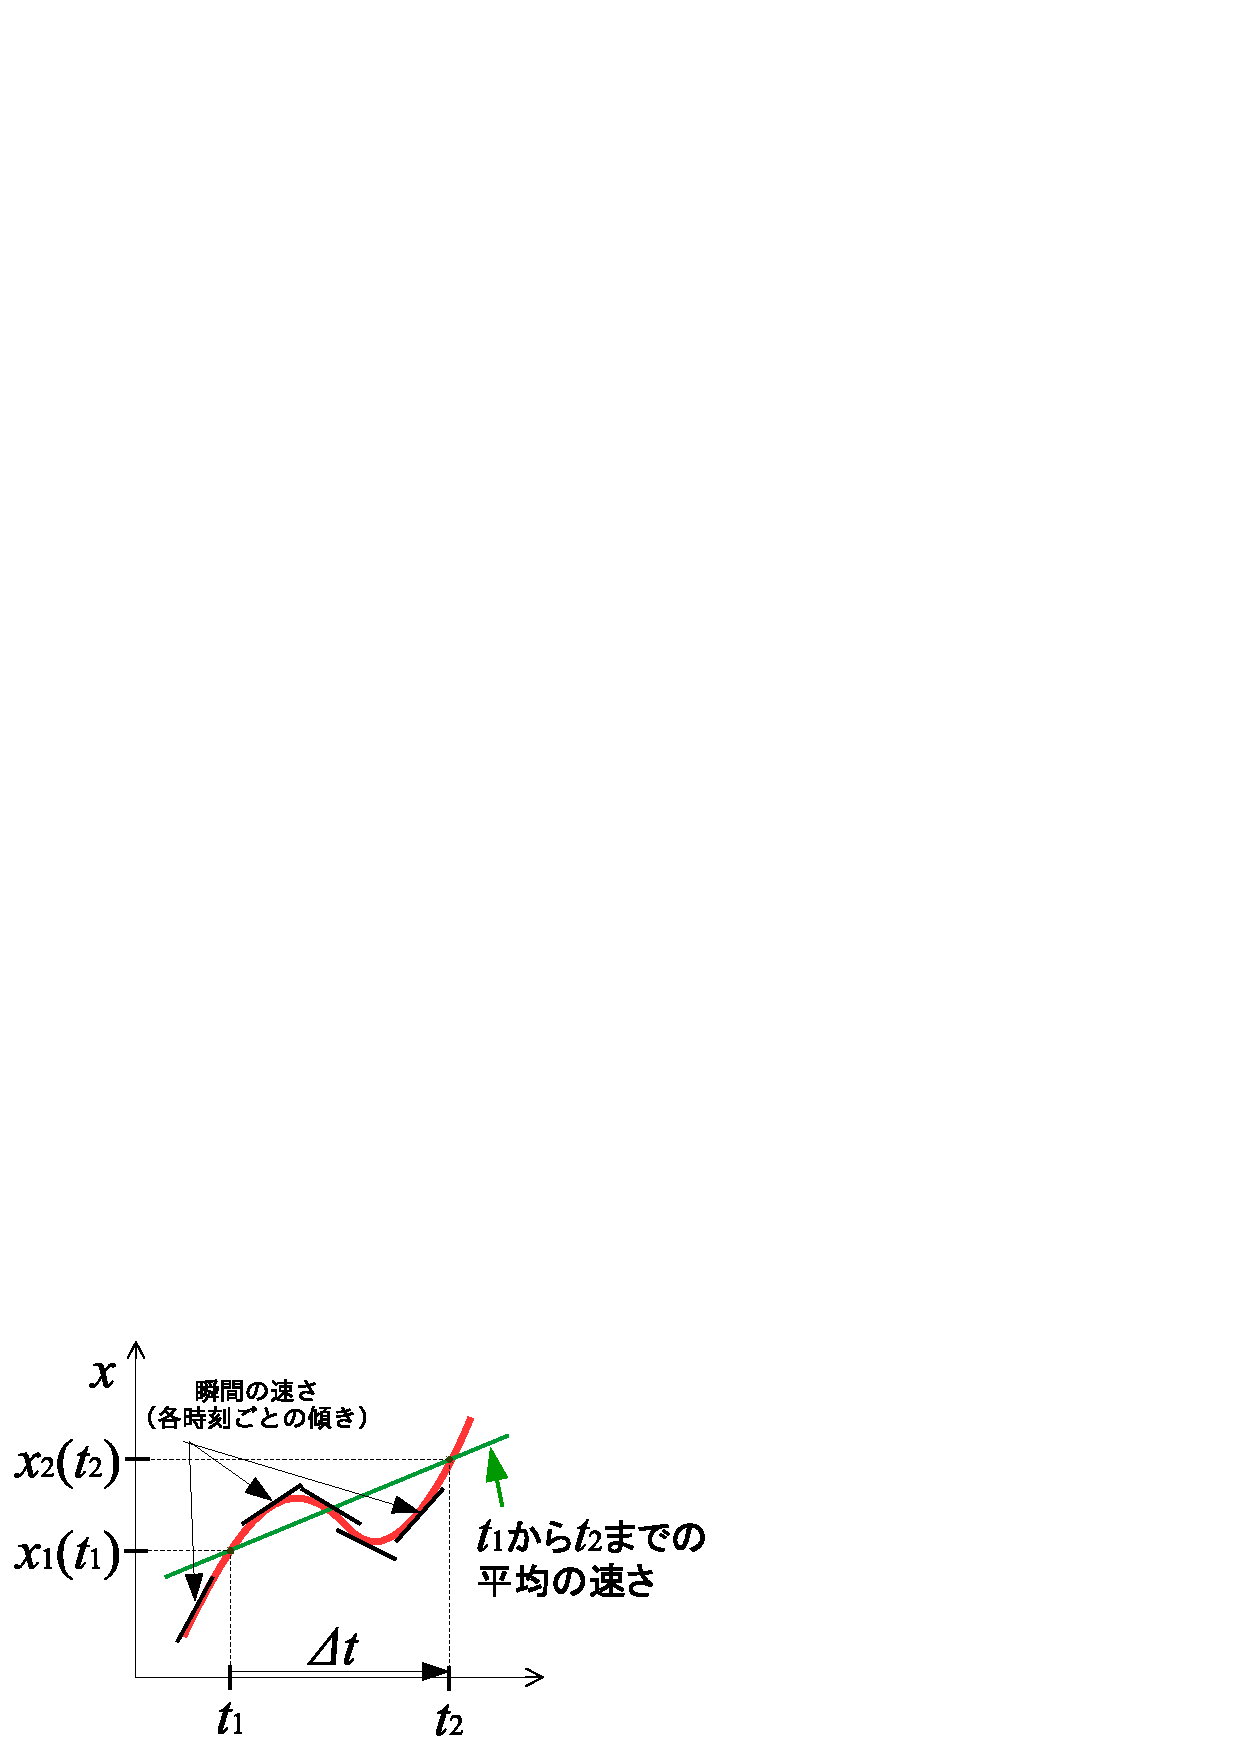
\includegraphics[keepaspectratio, width=7.2cm,height=3.88cm,clip]{Sokudo2.pdf}
                        \caption{速度2}
                        \label{fig:Sokudo2}
                    \end{center}
                \end{figure}

                実際の物体の速度は,各時刻で赤線の傾きであるのにもかかわらず,
                上の速さの式は,緑色の線の傾きというように
                みなされる.すなわち,
                位置 $x_{1}$ から位置 $x_{2}$ まで,
                速さが一定であるとみなされているのである.そのため,このままでは,
                ある特定の時刻における物体の速さが知りたいときには,
                速さの式は役に立たない.平均の速度だけしか考えることしか
                できないからである.

                そこで,次のように速さの式を
                いじってみる.例えば,時刻 $t_{1}$ を における
                物体の速度を知りたいとする.このとき,\textbf{時刻 $t_{2}$ を
                時刻 $t_{1}$ に近づけていけば,時刻 $t_{1}$ における
                物体の速度を得られる.}$\Delta t=t_{2}-t_{1}$ の関係式から,
                $t_{2}$ について解けば,
                \begin{align}
                    t_{2}=t_{1}+\Delta t
                \end{align}
                である.
                従って,時刻 $t_{2}$ を時刻 $t_{1}$ に近づけるとは,
                $\Delta t$ を0に近づけることと同じである.
                ところで,$\Delta t$ を0に近づけると,
                それに伴って位置も変化してしまう.位置の変化分は,
                $\Delta x=x_{2}-x_{1}$ であった.時刻を含めて
                詳しく書くと,
                \begin{align}
                    \Delta x=x(t_{2})-x(t_{1})
                \end{align}
                である.さらに,$t_{2}=t_{1}+\Delta t$ であるから,
                \begin{align}
                    \Delta x=x(t_{1}+\Delta t)-x(t_{1})
                \end{align}
                のように書ける.以上により,平均の速さの式は
                \begin{align}
                    v   &= \frac{\Delta x}{\Delta t}=\frac{x_{2}-x_{1}}{t_{2}-t_{1}}  \notag \\  \notag \\
                        &= \frac{x(t_{1}+\Delta t)-x_(t_{1})}{t_{1}+\Delta t-t_{1}} \notag \\  \notag \\
                        &= \frac{x(t_{1}+\Delta t)-x(t_{1})}{\Delta t}
                \end{align}
                のように変形できる.一般には,時刻 $t_{1}$ は任意の時刻で捉えることができるので,
                添え字の1をおとし,任意性を強調し,
                \begin{align}
                    v=\frac{x(t+\Delta t)-x(t)}{\Delta t}
                \end{align}
                と書ける.
                この式で,$\Delta t$ を0にもっていくのである.
                これを次のように表現する.
                \begin{align}
                    v=\lim_{\Delta t \to 0}\frac{x(t+\Delta t)-x(t)}{\Delta t}
                \end{align}
                この式の右辺を以下のように略記する.
                \begin{align}
                    \frac{\df x}{\df t}:=\lim_{\Delta t \to 0}\frac{x(t+\Delta t)-x(t)}{\Delta t}
                \end{align}
                この記号を用いて,速度は
                \begin{align}
                    v=\frac{\df x}{\df t}
                \end{align}
                のように表現する.但し注意することは,$\Delta t\not= 0$ を
                必ず満たしておくということである.

                図形的に考えると図\ref{fig:hayasa3}のようになる.
                \begin{figure}[hbt]
                    \begin{center}
                        \includegraphics[keepaspectratio, width=7.2cm,height=5.73cm,clip]{hayasa3.pdf}
                        \caption{速度3}
                        \label{fig:hayasa3}
                    \end{center}
                \end{figure}

                このような図を“$x-t$ グラフ”という.
                時刻 $t_{2}$ を時刻 $t_{1}$ に
                近づけると,直線の傾き $v$ はある一定の値になる.この直線は
                水色の線で描いた.$t_{a}$ を $t_{1}$ へ
                近づいていくと,それに伴って $x_{a}$ も
                位置 $x_{1}$ へと近づいていく.但し,
                $x_{a}$ は $x_{1}$ に重ならないようにしなければならない.
                この直線が時刻 $t_{1}$ における
                瞬間の速さとなるのである.

                ここで注意しておく.それは,物体の位置と時刻の組 $(x(t),\,t)$ が
                2つ分かっていないと,速さはわからないということである.
                このことを考慮しないと,パラドクスを生んでしまうことになる.
                そのパラドクスとは,「飛ぶ矢のパラドクス」として有名である.
                次のようなものである.\\
                \begin{itembox}[l]{飛ぶ矢のパラドクス}
                動いている矢は,ある時刻を指定すれば,それに対応してある特定の
                位置で静止しているはずである.
                \end{itembox}\\

                簡単にいえば,ある時刻に撮った飛ぶ矢の写真を見ると,
                その矢は静止しているように見えるということである.
                しかし,2つの時刻で2つの位置の飛ぶ矢の写真をとれば,
                飛ぶ矢の平均の速度が求まる.もちろん,
                シャッターを押す速さが非常に速ければ,
                瞬間の速度を求められる
                \footnote{
                実際は
                そのようなことをせず,
                ビデオカメラを使うだろうが.}.

                さて,今までは速度の方向について何も考えてこなかったが,
                これは,正と負で表現できる.すなわち,左から右へ
                物体が移動するときに,物体は正方向に速度をもつ
                といい,逆に右から左に物体が移動するときには
                物体は負の向きに運動するという.


%       %======================================================================
%       %  SubSection
%       %======================================================================
        \subsection{2次元(平面)上の速度}
            2次元上,すなわち平面上における
            物体の位置は2つの方向で考える.この物体の位置は $\br=(x,\,y)$ のように
            表現される.    その速度についても2つの方向を考える必要がある.
            $x$ 方向の速度を $v_{x}$ また,$y$ 方向の速度 $v_{y}$ と
            したとき,$\bv=(v_{x},\,v_{y})$ である.
            これらはそれぞれ1次元における速度と同じように考えられて,
            \begin{align}
                v_{x}=\frac{\df x}{\df t}:=\lim_{\Delta t \to 0}\frac{x(t+\Delta t)-x(t)}{\Delta t} \notag \\
                v_{y}=\frac{\df y}{\df t}:=\lim_{\Delta t \to 0}\frac{y(t+\Delta t)-y(t)}{\Delta t}
            \end{align}
            である.

            ところで,位置が $\br=(x, y)$ と表せるので,
            速度は以下のようにも表せる.
            すなわち,
                \begin{align}
                    \bv=\left(v_{x} , v_{y}\right)
                       =\left(
                           \frac{\df x}{\df t},
                           \frac{\df y}{\df t}
                        \right)
                \end{align}
            である.


%       %======================================================================
%       %  SubSection
%       %======================================================================
        \subsection{3次元(空間)内の速度}
            3次元への拡張は容易だろう.3次元における物体の位置
            を $\br=(x,\,y,\,z)$ として,
            速度を $\bv=(v_{x}\,,\,v_{y}\,,v_{z})$ とすればよい.
            復習を兼ねてもう一度,形式的に速度について確認していく.

            時間が $t$ から $\Delta t$ だけ時間が経過したとき,
            位置は $\br(t)$ から $\br(t+\Delta t)$
            に変化する.すなわち,平均の速度 $\bar{\bv}$ は
                \begin{align}
                    \bar{\bv}
                    &= \frac{\br(t+\Delta t)-\br(t)}{t+\Delta t -t} \notag \\
                    &= \frac{\br(t+\Delta t)-\br(t)}{\Delta t }
                \end{align}
            である.知りたいのは「瞬間の速度」である.
            「瞬間の速度」を考えるために $\Delta t$ を0近づける.すると,
                \begin{align}
                    \bv
                    = \lim_{\Delta t \to \infty}\frac{\br(t+\Delta t)
                    -\br(t)}{\Delta t} \notag \\
                \end{align}
            となる.従って,
                \begin{align}
                    \bv=\frac{\df \br}{\df t}
                \end{align}
            である.これが \textbf{瞬間の速度} である.速度の単位は,[m/s] である.

            ところで,位置が $\br=(x, y, z)$ と表せるので,
            速度は以下のようにも表せる.
            すなわち,
                \begin{align}
                    \bv=\left(v_{x} , v_{y} , v_{z}\right)
                       =\left(
                           \frac{\df x}{\df t},
                           \frac{\df y}{\df t},
                           \frac{\df z}{\df t}
                        \right)
                \end{align}
            である.

            \begin{memo}{速度のを表す他の記号}
            速度は,$\df \bv/\df t$ と表現した.しかし,これを簡略化をして,以下のように書くことも
            あるので注意すべきだ.
                \begin{align}
                    \dot{\br} := \frac{\df \textit{\textbf{}v}}{\df t}.
                \end{align}
            \end{memo}

%       %======================================================================
%       %  SubSection
%       %======================================================================
        \subsection{速度の合成}
            今,人間 $A$ が速度 $\bv_{A}$ の等速で運動をしているとする.
            このとき,$A$ は 物体が速度 $\bv_{\mbox{物体}}$ をもって運動している のを見たとする.
            自分から見た物体の速度 $\textit{\textbf{V}}$ はどのようになるかを計算する.
            これは,ガリレイの \textbf{速度の合成則} によると,
                \begin{align}
                    \textit{\textbf{V}}=\bv_{\mbox{物体}}-\bv_{A}
                \end{align}
            の関係がある.この関係は,速度のベクトル和として考えられることによる.
            このように,$A$ から見た相手の速度 $\textit{\textbf{V}}$ のことを \textbf{相対速度} という.
            自分の速度を基準に, $\bv_{A}=0$ としたとき,
             $\textit{\textbf{V}}=\bv_{\mbox{物体}}$ となる.すなわち,
             自分は静止していて,動いているのは物体である主張できる.

            逆に,別の人 $B$ が物体の上から$A$を見るときを考える.$B$ は物体と共に運動している
            ことから,$\bv_{\mbox{物体}}=0$ とみなす.従って,動いているのは,$A$ であると主張できる.
            つまり,観測者によって 観測者自身の速度 が異なるので,物体の速度は 観測者によって 異なって見えるのである.
            (ここでは,観測者の立場によって,物体が動いていたり,止まっていたりしていた.)観測者の立場によって,
            互いの速度の主張は逆である.これが相対速度といわれる理由である.
            とすると,このままでは“絶対に正しい”とできる速度が存在しないことになる.
            従って,今まで,「速度」とか「加速度」とかという言葉を使ってきたが,何に対する 速度 または 加速度 であるのかを全く
            断っていなかった.この「何に対する」の『何』にあたるものが,速度や加速度の基準である.
            \begin{figure}[hbt]
                \begin{center}
                    \includegraphics[keepaspectratio, width=7.2cm,height=5.92cm,clip]{soutaisokudo.pdf}
                    \caption{相対速度(Aから見た物体の速度 と Bから見た物体の速度)}
                    \label{fig:soutaisokudo}
                \end{center}
            \end{figure}

            \begin{memo}{数式と実際の現象}
                いよいよベクトルや微分,さらにはベクトルの微分と,数式が出てきは
                じめた.
                最初に戸惑うのは,数式と数式で表現されている現象との関係だろう.
                あたりまえのようだが,これについては問題を解くなりしていくしかない.
                物理学は実際の現象を数式で表す.逆にいえば物理における数式は何らかの
                物理現象を表現していると言える.式を見て,その式の内容を具体的な例で
                イメージできるように
                なるとよい.例えば,位置 $\br$ と表現されていたら,この具体的なイメ
                ージは,
                自分が原点に立っていて,その位置を指で示していることを考えればよい.
                速度 $\bv$ といわれたら,
                一定の速度で走る自転車を思い浮かべればよい.一定の速度で走るということは,
                常に時間変化 $\Delta t$ に対する自転車の変位 $\Delta\br$ が一定であることから,
                \begin{equation*}
                    \frac{\Delta \br}{\Delta t}=\mathrm{const(\mbox{一定})}=\bv
                \end{equation*}
                ということである.時間微分は,ある量(ここでは変位$\Delta \br$)時間変化に
                対する変化の割合を
                表現している.このように,式と現象が自身の中で,具体例を持って認識できる
                ようになるとよい.
            \end{memo}


%   %==========================================================================
%   %  Section
%   %==========================================================================
    \section{加速度の表現方法}
        \begin{mycomment}
            \textbf{加速度} とは,速度の時間変化具合を表す量である.
            速度を考えた時と同様に,加速度も1次元の場合から3次元の場合と,
            順を追って考えてくことにしよう.
        \end{mycomment}

%       %======================================================================
%       %  SubSection
%       %======================================================================
        \subsection{1次元(直線)上の加速度}
            一次元,つまり,直線的に運動する物体の速度 $v_{x}(t)$ は
            位置 $x(t)$ の時間変化 $\df / \df t$ として定義された.
            定義された.定義式は次の通りであった.
                \begin{align}
                    v_{x}(t) := \frac{\df x(t)}{\df t}
                              = \lim_{\Delta t \rightarrow 0}\frac{x(t+\Delta t)-x(t)}{\Delta t}.
                \end{align}

            ここでは更に,“速度の時間変化”を考える.この速度の時間変化を \textbf{加速度} と
            いう.以下に加速度を定義していこう.

            ある時刻 $t_{0}$ における物体の速度を $v_{x0}$ としたとき,
                \begin{equation*}
                    v_{x0} = v_{x}(t_{0})
                \end{equation*}
            という式が成り立つ.そして,次の時刻 $t_{1}$ における物体の速度 $v_{x1}$ は,
                \begin{equation*}
                    v_{x1} = v_{x}(t_{1})
                \end{equation*}
            と書ける.つまり,時刻 $t_{0}$ から $t_{1}$ までの間に,
            物体の速度は $v_{x0}$ から $v_{x1}$ に変化したことになる.
            時刻の変化(時間)を $\Delta t$,速度の変化を $\Delta v$ とし,
                \begin{align*}
                    \Delta t &= t_{1}  - t_{0}   \\
                    \Delta v &= v_{x1} - v_{x0}
                \end{align*}
            と置けば,加速度 $a_{x}$ は以下のように定義できる.すなわち,
                \begin{align}
                    a_{x} := \frac{\Delta v}{\Delta t}
                \end{align}
            である.これにより,加速度が速度の時間変化で定義されることが,
            示せた.

            もう少し,加速度の定義式を具体化していこう
                \footnote{
                    今まで置いた文字を展開していくことになる.効率の悪い説明だが,気にしない.
                }.
                \begin{align*}
                    a_{x} &= \frac{\Delta v}{\Delta t}                     \\
                          &= \frac{v_{x1} - v_{x0}}{\Delta t}              \\
                          &= \frac{v_{x}(t_{1}) - v_{x}(t_{0})}{\Delta t}  \\
                          &= \frac{v_{x}(t_{1}) - v_{x}(t_{0})}{\Delta t}  \\
                          &= \frac{v_{x}(t_{0}+\Delta  t) - v_{x}(t_{0})}{\Delta t}.
                \end{align*}
            ここで,$\Delta t = t_{1} - t_{0}$ から $t_{1} = t_{0}+\Delta  t$ を使った
                \footnote{
                    書くまでもないか$\cdots$.
                }.
            最後に,右辺に対して,$\Delta t \rightarrow 0$ の極限をとろう.
                \begin{align}
                    a_{x} = \lim_{\Delta t \rightarrow 0}
                            \frac{v_{x}(t_{0}+\Delta t) - v_{x}(t_{0})}{\Delta t}.
                \end{align}
            時間 $t$ による微分の記号 $\df/\df t$ を使うことで,速度が正確に定義できるようになった.
            すなわち,
                \begin{align}
                    a_{x}    :=\frac{\df v_{x}(t)}{\df t}
                              =\lim_{\Delta t \rightarrow 0}
                               \frac{v_{x}(t_{0}+\Delta t) - v_{x}(t_{0})}{\Delta t}.
                \end{align}

            更に一般化しよう.今までは,時刻 $t_{0}$ における物体の加速度を求めていたが,
            これを任意の $t$ で置き換えよう.
            そして,改めて,今度は正式に,加速度を次式で定義しよう.
                \begin{align}
                    a_{x}(t) :=\frac{\df v_{x}(t)}{\df t}
                              =\lim_{\Delta t \rightarrow 0}
                               \frac{v_{x}(t+\Delta t) - v_{x}(t)}{\Delta t}.
                \end{align}
            上式で,左辺の加速度の表現に,時刻 $t$ が独立変数であることを,
            明記するようにした.

            \begin{memo}{速度$\cdot$位置$\cdot$加速度の関係}
                速度 $v_{x}(t)$ が,$v_{x}(t) := \df x/ \df t$ と定義
                されるので,次の関係が成立している.
                \begin{align}
                    a_{x}(t) := \frac{\df v_{x}(t)}{\df t} := \frac{\df^{2} x(t)}{\df t^{2}}.
                \end{align}
                加速度の表現として,
                    \begin{equation*}
                        \frac{\df^{2} x(t)}{\df t^{2}}
                    \end{equation*}
                というものが,最もよく用いられる.

                「加速度は,位置に関する二階微分で定義される」という(見たまんまだ).
            \end{memo}

%       %======================================================================
%       %  SubSection
%       %======================================================================
        \subsection{2次元(平面)上の加速度}
            二次元の場合の加速度も,次元が増えただけで,考えることは一次元の
            場合と同じ.違いは,一次元の場合は1方向($x$ 軸)のみで考えればよ
            かったところを,二次元の場合は,2方向($x,\,y$)を考慮する点のみ.

            2つの方向を $x$ 軸,$y$ 軸とする.$x$ と $y$ 軸はそれぞれ独立だから,
            2つを別々に考えれば良い.どの方向を向いても,加速度の定義を変更する
            必要はない
                \footnote{
                    \textbf{空間の等方性} より.空間の方法性とは,
                    どの向きに運動しようが,その物体に対する
                    物理法則は不変である,という仮説のことを言う.
                }.
            つまり,1方向で考えたことが,そのまま残りの方向にも成立するということ
                \footnote{
                    してもらわないと困る.というか,成立するものとして,定義される.
                }.

            なので,上で考えた1次元の場合の式を,2方向に適用するだけで良い.
            次のように2方向の場合の加速度が定義できる.
                \begin{align}
                    \ba (t) := \frac{\df \bv(t)}{\df t}
                             = \left(
                                   \frac{\df^{2} x(t)}{\df t^{2}},\,\;
                                   \frac{\df^{2} y(t)}{\df t^{2}}
                               \right).
                \end{align}

            ただし,表記上の問題として,位置$\cdot$速度$\cdot$加速度
            をベクトル表記(太字)にした.

%       %======================================================================
%       %  SubSection
%       %======================================================================
        \subsection{3次元(空間)内の加速度}
            3次元になろうが,やることはこれまでと同じ.
            3次元空間内における加速度を $\textit{\textbf{a}}$ と表すと,
                \begin{align}
                    \textit{\textbf{a}} := \frac{\df \bv}{\df t}
                \end{align}
            である.考え方は速度のときと同じである.
            つまり,加速度とは速度の時間変化のことである.
            速度が時間の経過とともに速くなったり,逆に遅く
            なったりしたとき,
            その変化の具合が加速度である.

            また,速度の定義式から,以下のようにも加速度を表せる.
            すなわち,
                \begin{align}
                    \textit{\textbf{a}} &= \left( a_{x} , a_{y} , a_{z} \right) \notag \\
                    &= \left( \frac{\df v_{x}}{\df t} , \frac{\df v_{y}}{\df t} ,\frac{\df v_{z}}{\df t} \right)  \notag \\
                    &= \left( \frac{\df^{2}x}{\df t^{2}},  \frac{\df^{2}y}{\df t^{2}},  \frac{\df^{2}z}{\df t^{2}} \right) \notag \\
                    &= \frac{\df^{2}\br}{\df t^{2}}
                \end{align}
            とも表現できる.
            加速度が正の場合は,速度が上がっていくことを意味する.
            また,加速度が負の場合は,速度が下がっていくことを意味する.
            もちろん,加速度が 0 であれば,速度変化はないということである.

            加速度の単位は $[\rm{m/s^{2}}]$ である
                \footnote{
                    $[\rm{m/s^{2}}]$ はメートル毎秒毎秒とよむ.
                }.

            \begin{memo}{変化の記述}
                上に,「数式と物理現象は互いに関連していている」
                というようなことを書いた.そして,数式を見たときに,
                「それを現象を具体的な例で想像できることが大切である」
                とも書いた.しかし,具体的に式をイメージする方法を
                示していなかった.そこで,ここではこの例
                    \footnote{
                        当然,ここで紹介するのは,その単なる一例であり,これが全てではない.
                        むしろ,人ぞれぞれで,想像の仕方が異なっているはずである.
                        従って,想像できるようであれば,この節を読みとばしてかまわない
                        -----むしろ混乱するだろうから,読み飛ばすべきかも知れない.
                    }
                として,また,今までの復習を兼ねて,
                いまの私の考える微積分と物理現象を考えたい.


                物体は大きさをもっているが,この物体の運動を考えるときには物体の大き
                さを無視したほうが計算上都合がよい.
                物体の重心の運動を追うことで,物体の運動の軌跡を得ることができる.
                物体をこの重心部分にギュギュ!!と押しつぶして
                大きさをなくした点を考える.このような点のことを \textbf{質点} という.
                力学では,剛体の場合を除いて,物体の運動を考える
                ときは,質点の運動のことを考える.以下では,「物体」と書かれていたのなら,
                それは,特に断りのない限り,質点と同義であるとする.

                物体の運動を語るには,最初に,物体の \textbf{位置} を表現しなければならない.
                物体の位置は \textbf{座標} を用いて表現される.
                簡単のために,自身の居る点を原点 O にとろう.
                位置を表す記号として,$\br$ と表現する.つまり,物体の位置は
                \begin{equation*}
                \br =(\,x\,,\,\,y\,,\,\,z\,)
                \end{equation*}
                のように表現される
                \footnote{
                座標としては直交座標でないといけないという制約はないが,ここでは一番わか
                りやすいと思われる
                座標としてこの座標をとった.
                }.位置については,そのイメージをすることは容易だと思う.自分が原点にいて
                ,その点を指でさしている,というイメージ
                をすればよい.

                次に,物体の \textbf{速度} を考える.物体の速度とは,位置の時間変化を表す量である.
                まず,“変化”をどのように数式で表現すればよいかを考える.
                量の変化を表すには,その変化の前と後で二つの量の差を考える必要がある.量の変化は,
                \begin{equation*}
                [\mbox{量の変化分}] = [\mbox{変化後の量}] - [\mbox{変化前の量}]
                \end{equation*}
                と計算される.上の式をもう少し格好をつけて書くと,量の変化分を表すときには,
                その量を表す記号の前に $\Delta$ を
                つける.変化する量を,例えば $x$ としたとき,変化分は $\Delta x$ と表現する
                \footnote{
                $\Delta$ は,デルタ と読む.
                }
                .従って,変化前の量を $x_{\mbox{変化前}}$,
                変化後の量を $x_{\mbox{変化後}}$ と表現すれば,
                \begin{equation*}
                \Delta x = x_{\mbox{変化前}} - x_{\mbox{変化後}}
                \end{equation*}
                となる.

                また,「Aに対するB」を考えるとき,これは比で表現できて,
                \begin{equation*}
                \frac{B}{A}
                \end{equation*}
                と数式表現できる.例えば,二人の子どもに,3つのクッキーを配るとしよう.子ども一人
                に対して,
                クッキーはどれくらい与えられるかを考えれば,3/2 個であることは容易に計算される.
                この 3/2 は,
                \begin{equation*}
                    \frac{3[\mbox{個]}}{2[\mbox{人]}}
                \end{equation*}
                という意味である.式の意味は,「子ども二人に対して,クッキーが3つ」である.これは,
                子ども一人あたりのクッキーの個数でもある(3/2[個/人]).

                変化を考えるとき,基本となるのはこの引き算と割り算であり,
                後はこの組み合わせである.
                変化の基準となるものを分母にし,変化の対象となるものを分子におく.
                具体的に表現するならば,
                \begin{equation*}
                    \frac{\Delta A}{\Delta x} = \frac{A(x_{2})-A(x_{1})}{x_{2}-x_{1}}
                \end{equation*}
                のようである.$x$ の関数である $A(x)$ を考えるとき,$x$ の変化 $\Delta x$ に対
                する $A$ の変化 $\Delta A$ が
                上式で表現されている.現象の変化を表す一般的な形は,この式のようになる.


                やっと速度について考えられるが,
                速度の定義は,時間変化 $\Delta t$ の間にどの程度位置の変化 $\Delta x$ が起こるかを
                表現する.つまり,時間変化 $\Delta t$ に対する位置の変化 $\Delta x$ であるから,
                \begin{equation*}
                \frac{\Delta x}{\Delta t}
                \end{equation*}
                と表現される.
                この式は,次のように考えるとよい.まず,時間 $\Delta t$ を1秒で一定としてみよう.
                このとき,一秒で進む距離が大きければ大きいほど速度が速くなることをこの式は表現する.
                私達の経験上においても矛盾はないだろう.また,逆に,位置の変化 $\Delta x$ を1メー
                トルで一定にして
                考えてみよう.この場合,1メートルを進む時間が短ければ短いほど速度が速くなる.1メー
                トルを1秒で
                進みのと,1メートルを0.1秒で進むのでは,完全に後者の方が速い.

                実際の速度の変化は,直交座標でいうところの,$x$,$y$,$z$ の3方向で変化する.
                これは,位置が3方向であることから,当然のことである.従って,速度も3つの向きをもつ.
                つまり,
                速度もまたベクトルである.

                式で速度に意味をもたせる時には,それに対応した文字を割当てるとよい.そこで,速度
                を表現する記号として,$\bv$ を
                使うことにしよう.このノートでは,「定義する」という意味をこめて,$:=$ を使う.
                その使用方法は,例えば,記号Aに
                Bという意味をもたせたい時に,「AをBというように定義する」というとき,A$:=$Bのよ
                うに書く.今の速度の定義の場合,
                記号Aに対応するのが $\bv$ であり,意味Bに対応するのが $\Delta \br/\Delta t$ であるか
                ら,速度の定義は次のように
                書き表される.
                    \begin{align}\label{sokudonosiki_1}
                        \bv := \frac{\Delta \br}{\Delta t}.
                    \end{align}

                しかし上の式では,前の項目で定義した速度の定義と記号が異なる.
                小さい変化という意味をこめて,$\Delta$ を使っている点である.
                この記号 $\Delta$ は有限の個数の範囲でたくさん分割したときの,その1つの区間という
                イメージで使用される.
                しかし,これはあくまでも近似的な考えである.理想的には分割個数を無限大にし,分割さ
                れた区間を無限小にしたい.
                そこで,微積分という手段を使う.
                微積分を用いることで,無限小の変化を扱うことができる.有限分割から無限分割にしたの
                で,当然,
                用いる記号も
                変えないといけない.すなわち,$\Delta$ を $\df$ に変えるということである.
                    \begin{align}\label{sokudonosiki_2}
                        \bv := \frac{\df \br}{\df t}.
                    \end{align}
                式(\ref{sokudonosiki_1})と式(\ref{sokudonosiki_2})の違いは,位置の変化を有限分割に
                して表すか,
                無限分割にして表すかの違いである.速度の定義は,無限分割の概念で定義するほうが適当
                であるから,
                式(\ref{sokudonosiki_2})が正式な速度の定義になる.

                上記はベクトルで書かれているが,これは,単なる以下の式の省略である.
                        \begin{align}
                            \left(
                                v_{x} ,\,
                                v_{y} ,\,
                                v_{z}
                            \right)
                            = \left(
                                \frac{\df {r}_{x}}{\df t} ,\,
                                \frac{\df {r}_{y}}{\df t} ,\,
                                \frac{\df {r}_{z}}{\df t}
                              \right)
                        \end{align}
            \end{memo}


    \section{躍度(加加速度,jerk)}\label{seq:jerk_define}
        理論構築には直接的に関係がないためか,力学の教科書では見かけないけど,
        加加速度(jerk)についても書いておこう.
        現実的には,加速度も時間変化する.この加速度の時間変化を \textbf{加加速度} という.
        \textbf{躍度} ともいう.個人的には,躍度という方を好む
            \footnote{
                加加速度だといい間違えたと思われて誤解されそうなので.
            }.
        英語だとjerk(ジャーク).躍度は,工学的な匂いが強い.

        一応式も書いておこう.加速度がベクトルであるから,躍度もベクトルになる.
        躍度を現す記号を$\bj$としよう
            \footnote{
                jerkからとったjである.後に使う仕事の記号jとは無関係.電気数学の虚数単位とも無関係.
            }.
        定義式は以下.
            \begin{align}\label{eq:jerk_define}
                \bj &:= \frac{\df \ba}{\df t} \\
                    &=  \frac{\df }{\df t} \left(\frac{\df \bv}{\df t}\right) \notag \\
                    &=  \frac{{\df}^{2} \bv}{{\df t}^{2}} \notag \\
                    &=  \frac{{\df}^{2} }{{\df t}^{2}} \left( \frac{\df \bx}{\df t} \right) \notag \\
                    &=  \frac{{\df}^{3} \bx}{{\df t}^{3}}. \notag
            \end{align}






\chapter{3つの運動法則 と 万有引力の法則}
%   %-----------------------------------------------------------------------------------------------
%   %  Input
%   %    File Name : PhysNote_CM_LawKinemaGrav.tex
%   %    説明      : ニュートンの運動の3法則・万有引力の法則について,説明する.
%   %-----------------------------------------------------------------------------------------------
        %===================================================================================================
%  Chapter : 運動の法則と万有引力
%  説明    : ニュートンの運動の3法則・万有引力の法則について,説明する.
%===================================================================================================
\begin{mycomment}
    ニュートン力学は,4つの法則により成立している.
    4つの法則のうち,3つは物体の運動に関する法則(運動の3法則といわれる)であり,
    残りの1つは万有引力の法則である.
    物体は,この4つの法則を満たすように運動する.
    この章では,
    ニュートンの運動の3つの法則,万有引力の法則を説明していく.
\end{mycomment}
%   %==========================================================================
%   %  Section
%   %==========================================================================
    \section{運動の3法則}
%       %======================================================================
%       %  SubSection
%       %======================================================================
  \subsection{(第1法則)慣性の法則}
                力を与えられていない物体は,その動き方に変化は生じない.
                外力が加わらなければ,等速直線運動している物体は等速直線運動を続けるし,
                静止している物体は静止し続ける.
                このような性質を物体の運動の根本原因と考え,法則と捉える.
                この法則の名前を \textbf{慣性の法則} という
                \footnote{
                  「…し続ける」という性質を,\textbf{慣性} という.
                }.

                慣性の法則は実験によってのみ確かめることができ,
                どのような原理でこの法則が成立しているのかということを問題とはしない
                  \footnote{
                    問題にすることはできない,と言ったほうがよい.物理学は自然現象を論理的に説明
                    する学問である.論理的説明をするには,説明なしに受け入れなければいけない約束事
                    を設ける必要がある.これを数学では \textbf{公理} というが,物理学でこの公理
                    に対応するものが \textbf{法則} と言われるものである.
                    慣性の法則は,このような説明なしに受け入れるべき法則の1つである.
                  }.

                まとめておこう.
                \begin{myshadebox}{慣性の法則}
                    物体の運動に関する次のような性質を,\textbf{慣性の法則} という.
                    \begin{itemize}
                        \item 座標系 $S$ に対して静止している物体は,
                              外力が加わらない限り,$S$ に対して静止し続ける.
                        \item 座標系 $S$ に対して速度をもっている物体は,
                              外力が加わらない限り,$S$ に対してその速度を保ち続ける.
                    \end{itemize}
                \end{myshadebox}
                \begin{figure}[hbt]
                    \begin{center}
                        \includegraphics[keepaspectratio, width=4.8cm,height=2.0cm,clip]{kanseinohousoku.pdf}
                        \caption{慣性の法則}
                        \label{fig:kanseinohousoku}
                    \end{center}
                \end{figure}

                この法則によって,慣性系の存在が暗黙的に仮定される
                    \footnote{
                        もっとストレートに「慣性系が一つ存在する」と表せばよいのだが,どの教科書を見ても,
                        何故か,そう書かれていない.このノートもその例に従っている.
                        確かに,等速運動を続けるとか静止し続けると書いたほうが,直感的にわかりやすい.
                    }.
                「速度をもつ」とか「加速度をもつ」とかという場合,基準となる慣性系が必要だからである.
                相対速度の項目で確認したように,観測者の見る物体の速度は,
                観測者と物体間の相対速度である.すなわち,同じ物体を見ているのにもかかわらず,
                別の速度で運動している観測者にっとっては,物体は全く異なった速度として観測される.
                極端な例では,物体と同じように等速直線運動する座標系から物体を見た場合は,
                その物体は静止しているとみなされる.つまり,座標系によって物体の速度が異なってしまう.
                そこで,等速直線運動する全座標系から一つ基準となる慣性系を選び,
                この座標系を特別な座標系として扱うのが最も自然である.
                選び出された1つの座標系は速度をもっていないとみなされ
                  \footnote{
                    基準となる座標系に速度がなければ,理論的に整った(補正項のいらない)説明ができる.
                    その他の座標系は,この基準となる座標系に補正項を加えた形で表現することができる.
                  },
                これは \textbf{絶対静止系} とよばれる.

                上記の慣性の法則で言っている座標系 $S$ とは,絶対静止系のことである.
                力学は絶対静止系を,速度や加速度,力の基準として構築されている
                    \footnote{相対性理論によると,絶対静止系 $S$ の存在は否定されるが,
                        ニュートン力学を考える範囲では系 $S$ の存在を仮定したうえで成立する
                        理論である.認めてもその理論に支障はない.
                    }.

                以下では,単に速度とか加速度とかと書いた場合は,それは系 $S$ に対するもの
                であると考える.
                ちなみに,車や電車の速度の基準は,地球を基準(絶対静止系)とした場合のものである
                  \footnote{
                    地球は太陽の周りを公転しているので静止していないではないか,という反論が
                    あるかもしれないが,実際には私達は地球が静止しているように感じており,こう考えても
                    実使用上は問題はない(物理理論的には問題だが,工学的には有効な考え方である).
                    絶対静止系を任意に取れることを身近な例によって示したかったので,地球を例にした.
                  }.

                絶対静止系は等速直線運動している全座標系から任意にひとつだけ選びとった座標系であるので,
                等速度運動状態と静止状態が全く同等である.

                逆に,物体の動き方が変わった時(加速度が生じた場合)には,力が作用したと考える
                具体的には運動の第2法則(運動方程式)として記述される.
                物体に力が加わった場合,その物体は加速度が生じる.

%       %======================================================================
%       %  SubSection
%       %======================================================================
        \subsection{(第2法則)運動方程式}
                運動の第2法則は実際に動いている物体に対するものである.具体的には,
                重い物体は動かしにくく,軽い物体は動かしやすい.このようなイメージを
                式で表現する.

                物体の運動は以下の式によって記述できる.
                    \begin{align}\label{undouhouteisiki}
                        \frac{\df^{2}\br}{\df t^{2}} = k\frac{\bF}{m_{\mathrm{i}}}
                    \end{align}
                ここで,$k$は定数,$m_{\mathrm{i}}$ は \textbf{慣性質量} であり,
                $\bF$ は力 である.言葉でいうと,
                    \begin{center}
                『物体の加速度は 慣性質量に反比例し,力に比例する』
                    \end{center}
                である.これを \textbf{運動方程式} という.

                おそらく,歴史的には紆余曲折があって,最終的にこの形に落ち着いたのであろう.
                ニュートンが提示した最初の式は,微分積分学が整っておらず
                  \footnote{
                    ニュートンのこの力学の提示で,微分積分学が始まったとすれば,当然だ.
                    微分方程式という考え方はニュートンの力学以降に発展するのであり,
                    また,よりよい式表現のための記号法が整備されることになる.
                  },
                当然ながらこのような微分方程式の記述にはなっていなかったはず.
                式の形がこうなるまでの経緯は歴史的には重要かもしれないが,
                このノートでは興味のないことである.すでに数式的に整った形になっているのだから,
                これを積極的に受け入れるべきである.同じニュートンの運動法則を意味している
                のには変わりないのだから.

                運動方程式をもう少し整理し,わかりやすく書き換えよう.
                力の単位 $[\rm{N}]$ を$[\rm{N}] = [\rm{kg (m/s^{2})}]$ すると,
                定数$k$は $k=1$ になって,以下のように書ける.
                        \begin{myshadebox}{運動方程式}
                            ニュートンの運動方程式は,以下のように表現される.
                            \begin{align}\label{eq:N_eq}
                            m_{\rm{i}}\frac{\df^{2}\br}{\df t^{2}} = \bF
                            \end{align}
                        \end{myshadebox}
                        \begin{figure}[hbt]
                            \begin{center}
                                \includegraphics[keepaspectratio, width=6cm,height=6cm,clip]{ma_F.pdf}
                                \caption{運動方程式}
                                \label{fig:ma_F}
                            \end{center}
                        \end{figure}

                加速度は力に比例するので,その比例係数を慣性質量 $m_{\mathrm{i}}$ と見るのである
                    \footnote{
                        もともとあった比例定数 $k=1$ の記述は省略するが,
                        その理由が力の単位の取り方にあるということは覚えておくべきである.
                        これ以降でも様々な物理法則を表す式を見ていくが,比例定数が現れない
                        ことが多い.
                        これは理論的説明を簡潔に表現するべく,物理量の単位の定義を人為的に都合よく行っているからである.

                        単位の取り方によって,数値は変わってしまう(時には次元そのものも変わりうる)が,
                        これは物理的現象の本質ではない.物理現象を人間が説明しようとするときには,
                        ある視点からその現象を観測する必要がある.
                        観測するということは,その対象となる物理現象を偏った考えの下で見るということである.
                        こうなると当然ながら,同じ現象でも,観測方法の違いによって,測定結果がことなる場合が起こる.
                        しかし,間違いはどこにもない.どちらも正しい.同じ現象なのに,
                        測定方法によって異なる結果が出るのはおかしな気がするかもしれないが,受け入れるしかない.
                        1つの物理現象に対して,複数の物理学的説明があってもよいではないか.
                        理論は1つだけとは限らないの(人間は本当の物理法則を知ることはできない)と
                        考えるほうが健全な思考である.
                        このことは,学習を進めていくうえで忘れがちなので,ここで注意を促しておいた.
                    }.
                そうすれば「物体の質量が大きいほど,その物体に加速度をもたせるために必要な力は,
                大きくなる」と読み取れる.
                (力と加速度に具体的な数値を代入して確認してみるとよい.)
                すなわち,慣性質量は,「物体の動きにくさ」を表現していると考えられる.
                以下では,運動方程式として,式(\ref{eq:N_eq}) を用いることにする.

                運動方程式(\ref{eq:N_eq})は,慣性質量と加速度と力の3つの概念の関係を
                示しているだけであり,力の定義をなしているわけではないことに注意する.
                ここでは,とりあえず,「力」というものの存在を仮定しているのである.

                この法則で使われる等号は数学的に厳密な等号ではない.
                この法則は実験によって得られるものだからである.
                例えば,実験で加速度や慣性質量や力を
                測定するとき,必ず測定限界となる桁数が存在する.
                つまり,無限桁だけの測定はできないのだから,
                「ニュートンの運動方程式は小数点第○位の桁で正しい」としかいえない.
                すなわち,ニュートンの運動方程式(ニュートン方程式)における等号は,
                細かくいえば,近似を表すものである.
                しかし,物理では等号のようにして扱う.これによる不都合は
                ほとんどない.不都合が現れるのは量子力学や相対性理論で
                考える状況下においてである
                    \footnote{
                        相対性理論;光速に近い速度で動く物体を考える(特殊相対性理論).
                        一様でない重力が存在する空間を考える(一般相対性理論).
                        量子力学;原子レベルの大きさの粒子の運動の記述を考える.
                    }.
                そのときはニュートン方程式
                を書き換えてやればよい.このニュートン方程式は
                私達の目に見える物体の動きを
                かなりの精度で正確に記述できる方程式である.

%       %======================================================================
%       %  SubSection
%       %======================================================================
        \subsection{(第3法則)作用$\cdot$反作用の法則}
            2つの物体をもってきて,それぞれ名前をA,Bとする.
            このとき,\textbf{作用反作用の法則}とは以下のような法則のことである.
                \begin{myshadebox}{作用反作用の法則}
                    『物体Bが物体Aに力$\bF_{\rm{AB}}$を与えているとき,
                    物体Aも物体Bに$\bF_{\rm{AB}}$と大きさが同じで逆向きの力
                    $-\bF_{\rm{BA}}$を受けている』
                \end{myshadebox}
            \begin{figure}[hbt]
                \begin{center}
                    \includegraphics[keepaspectratio, width=6cm,height=6cm,clip]{sayou_hansayou.pdf}
                    \caption{作用$\cdot$反作用の法則}
                    \label{fig:sayou_hansayou}
                \end{center}
            \end{figure}

            これを式で表すと,
                \begin{align}
                    \bF_{\mathrm{AB}} = -\bF_{\mathrm{BA}}
                \end{align}
            である.この式を変形すると,
                \begin{align}
                    \bF_{\mathrm{AB}} +\bF_{\mathrm{BA}}= 0
                \end{align}
            となって,作用とその反作用で生じる力からの合計は 0 になることがわかる.
            作用とは,ここでは,力のことをいう.

            力いっぱい押してもビクともしない壁を,
            力いっぱい押してみよう.しかし,壁は動かない.
            壁に力を加えているのにその壁が動かないということは,
            ニュートン方程式に反していると,一見して見まちがえ得る.
            しかし,作用反作用の法則による,壁に押し返されていることを
            考えれば矛盾でもなんでもない.

            この法則は,「力」のもつ性質を記述している.
            この法則の対象は「力」そのものである.
            しかし,今までに「力」を明確に定義していないので,
            少々曖昧に聞こえてしまうかもしれない.
            実際,その通りである.この作用反作用の法則は他の2つの法則より
            も,何か違った雰囲気がある.この法則は
            「力とは何か」が分かったときに,
            削除されるものなのかもしれない.
            しかし,ここではそんな高度な質問に
            答えることは不可能であり,
            さしあたってはこの法則を受け入れて
            いくことにしよう.

            そうはいうものの,この法則は大切な法則である.
            この法則によって,物理学で重要な概念の1つである,
            保存則が導かれるからである.「保存する」とは時間に関係なく
            一定の値をとることをいう.
            保存則については後ほど詳しく考えていきたい.
            ここでは,作用反作用の法則は捨ててはならない重要な
            法則であるということをわかればそれでよい.

%       %======================================================================
%       %  SubSection
%       %======================================================================
        \subsection{慣性質量}
                運動方程式(第2法則)で現れた質量を \textbf{慣性質量} という.
                これは,すぐ後に説明する万有引力の法則に現れる質量
                    \footnote{
                        こっちは \textbf{重力質量} とよぶことになるが,詳細は後に述べる.
                    }
                と区別するための名前である.慣性質量の大きさの比べ方について,ここで
                学習しておこう.

                2つの質量があるとしよう.これらを $m_{i1}$,$m_{i2}$ とおく.
                この2つの質量に全く同じ力 $F$ を加えて,それぞれに加速度を与える.
                向きはあまり本質的でないので省略する.
                加速度が生じることは式(\ref{undouhouteisiki})によって保証されている.
                このときの各質点の加速度は,加わる力が一定でも質量が異なるので,
                互いに異なったものとなる.簡単のために,二つの質点は同一方向に
                運動するとしよう.各質点の加速度の大きさを $a_{1}$,$a_{2}$ とする.
                ここで加速度の向きも省略する.
                運動方程式(\ref{undouhouteisiki})によって,各質点の運動は以下のように記述される.
                    \begin{equation*}
                        a_{1}=k\frac{F}{m_{i1}}\,,\quad a_{2}=k\frac{F}{m_{i2}}
                    \end{equation*}
                この2つの式から共通の $F$ を消去すると以下の関係を得る.
                    \begin{equation*}
                        (kF=)\;a_{1}m_{i1}=a_{2}m_{i2}
                    \end{equation*}
                    \begin{equation*}
                        \frac{a_{1}}{a_{2}}=\frac{m_{i1}}{m_{i2}}
                    \end{equation*}
                慣性質量はこのように測定される.何か基準となる質量を1つ定めることによって,
                その他の質量を決定できる.キログラム原器の1[kg]が,その基準である.

                \begin{memo}{慣性の法則と運動方程式の関係}
                    運動方程式(\ref{eq:N_eq})は,慣性質量と加速度と力の3つの概念の関係を
                    示しているだけであり,力の定義をなしているわけではないことに注意する.
                    ここでは,とりあえず,「力」というものの存在を仮定しているのである.

                    この法則で使われる等号は数学的に厳密な等号ではない.
                    この法則は実験によって得られるものだからである.
                    例えば,実験で加速度や慣性質量や力を
                    測定するとき,必ず測定限界となる桁数が存在する.
                    つまり,無限桁だけの測定はできないのだから,
                    「ニュートンの運動方程式は小数点第○位の桁で正しい」としかいえない.
                    すなわち,ニュートンの運動方程式(ニュートン方程式)における等号は,
                    細かくいえば,近似を表すものである.
                    しかし,物理では等号のようにして扱う.これによる不都合は
                    ほとんどない.不都合が現れるのは量子力学や相対性理論で
                    考える状況下においてである
                        \footnote{
                            相対性理論;光速に近い速度で動く物体を考える(特殊相対性理論).
                            一様でない重力が存在する空間を考える(一般相対性理論).
                            量子力学;原子レベルの大きさの粒子の運動の記述を考える.
                        }.
                    そのときはニュートン方程式
                    を書き換えてやればよい.このニュートン方程式は
                    私達の目に見える物体の動きを
                    かなりの精度で正確に記述できる方程式である.
                \end{memo}



%   %======================================================================
%   %  Section
%   %======================================================================
        \section{万有引力の法則}
            \subsection{法則のイメージと数式による定義}
            万有引力の法則は,ニュートンの運動の3法則とは独立したものである.
            その内容は「2つの重力質量が存在しているとき,その両者は引き合う」というものである
                \footnote{
                    「重力質量」といったのは,先ほどニュートン方程式の部分で確認した
                    慣性質量とは別に定義される質量であることを示したかったからである.
                }.
            これはすなわち,2つのうちの一方の重力質量($m_{\rm{gA}}$ としよう)が他方の
            重力質量($m_{\rm{gB}}$ としよう)を
            引っ張るのである.もちろん,反対を考えれば,
            重力質量 $m_{\rm{gB}}$ が重力質量 $m_{\rm{gA}}$ を引っ張っていることになる.
            \begin{figure}[hbt]
                \begin{center}
                    \includegraphics[keepaspectratio, width=7.2cm,height=6.64cm,clip]{bannyuuinnryoku.pdf}
                    \caption{万有引力}
                    \label{fig:bannyuuinnryoku}
                \end{center}
            \end{figure}

            以上のことを,もう一度もう少しかしこまった言い方で確認しておこう.
            2つの重力質量 $m_{\rm{gA}}$,$m_{\rm{gB}}$ が存在すると,その重力質量
            同士が互いに引き合う.
            これが \textbf{万有引力の法則} である.
            以下の式は 重力質量 $m_{\rm{gA}}$が,重力質量 $m_{\rm{gB}}$ に引っ張られる力を表す.
            力と重力質量 の添え字に注意すること.
                \begin{myshadebox}{万有引力の法則}
                    万有引力(重力質量 $m_{\rm{gA}}$が,重力質量 $m_{\rm{gB}}$ に引っ張られる力)
                    は次式で定義される.
                    \begin{align}\label{Grav}
                        \bF_{\rm{AB}}
                        = -G\frac{m_{\rm{gA}}m_{\rm{gB}}}{{\left| \br_{A}
                        -\br_{B} \right|}^{2}}
                        \frac{\br_{A}-\br_{B}}{\left| \br_{A}
                        -\br_{B} \right|}.
                    \end{align}
                    ここに,$\br_{A}$,$\br_{B}$は,それぞれ$m_{\rm{gA}}$と$m_{\rm{gB}}$の 位置である.
                \end{myshadebox}

                \begin{figure}[hbt]
                    \begin{center}
                        \includegraphics[keepaspectratio, width=6.5cm,height=4.2cm,clip]{bannyuuinnryoku_rei2d.pdf}
                        \caption{万有引力(例:2次元)}
                        \label{fig:bannyuuinnryoku_rei2d}
                    \end{center}
                \end{figure}

            \begin{memo}{万有引力法則とケプラーの法則}
                ニュートンが万有引力の法則を見つけたのは,
                \textbf{ケプラーの惑星の運動の3法則} を
                説明するためであった.たしかに,
                万有引力をニュートンの運動の3法則を
                用いると,ケプラーの法則が満たされる.
                逆に,ケプラーの法則から万有引力を
                導ける.どちらを基本法則としてもよいと
                思われるが,ここは万有引力を
                基本法則としたほうが無難だろう---
                ケプラーの法則は3つであり,
                万有引力は1つであるから…これも思考経済だ---
            \end{memo}

            \subsection{重力質量}
            万有引力の法則で表される質量のことを,\textbf{重力質量} という.
            重力質量は,運動方程式で表される慣性質量とは,別の概念である.
            重力質量は物体の「重さ」を表現していると考えられる
                \footnote{
                    慣性質量とは,物体の動きにくさ を表すものであった.
                }.
            また,重力質量$m_{\rm{gB}}$が 重力質量$m_{\rm{gA}}$に引っ張られる力 $\bF_{\rm{BA}}$ は
                \begin{align}
                    \bF_{\rm{BA}}
                    =-G\frac{m_{\rm{gB}}m_{\rm{gA}}}{{\left| \br_{B}
                    -\br_{A} \right|}^{2}}
                    \frac{\br_{B}-\br_{A}}{\left| \br_{B}
                    -\br_{A} \right|}
                \end{align}
            である.
            $\bF_{\rm{AB}}$ と $\bF_{\rm{BA}}$ の関係は,明らかに
            ($\br_{B}-\br_{A}$の部分に注目)
                \begin{align}
                    \bF_{\rm{AB}}=-\bF_{\rm{BA}}
                \end{align}
            であることがわかり,作用反作用の法則が成立していることも確認できる.

            \begin{memo}{この世界にある「力」の種類}
            万有引力は基本的な力の1つである.基本的な力はこの他に3つあって,
            それは「電磁気的な力」,「弱い力」,
            「核力」である.力のことを \textbf{相互作用} ということもある.

             古典力学でいう力とは, 主に,電磁気的な力 と 万有引力 である.
            \end{memo}

            \subsection{重力加速度}
                万有引力の法則は,2つの物体間に関する法則である.
                ここで,違う視点から,万有引力の法則を眺めてみる.
                物体の一つを惑星,もう一方を任意の物体と考えてもらいたい.
                物体が惑星に引っ張られているイメージ.

                惑星の質量を,$M_{P}$,惑星の位置を $\br_{P}$ とする.
                    \footnote{
                        添字の $P$ は Planet の頭文字.
                    }.
                また,惑星上の物体の質量を $m_{\mathrm{g}}$,位置を $\br$ とする.

                すると,物体が惑星から受ける力は,以下の式で表せる.
                    \begin{equation*}
                        \bF
                        =-m_{\mathrm{g}}\left( G\frac{M_{P}}{{\left| \br-\br_{P} \right|}^{2}}
                        \frac{\br-\br_{P}}
                        {\left| \br-\br_{P}\right|}\right).
                    \end{equation*}
                ここに,$\br$,$\br_{P}$ はそれぞれ,質点の位置 と 惑星の位置 を表す.

                今基準としているのは惑星だから,惑星の位置を基準にすれば($\br_{P}=\bzero$),
                    \begin{equation*}
                        \bF
                        =-m_{\mathrm{g}}\left( G\frac{M_{P}}{{\left| \br \right|}^{2}}
                        \frac{\br}
                        {\left| \br\right|}\right).
                    \end{equation*}

                ここで,\textbf{重力加速度} を以下で定義する.
                        \begin{myshadebox}{重力加速度の定義}
                            次式で,重力加速度を定義する.
                            \begin{align}\label{eq:GravAccer000}
                                \textit{\textbf{g}} :=
                                G\frac{M_{P}}{{\left| \br \right|}^{2}}
                                \frac{\br}{\left| \br \right|}.
                            \end{align}
                        \end{myshadebox}

                万有引力の法則に,惑星の質量 $M_{P}$,惑星の位置 $\br_{P}=\bzero$ を代入している.
                この定義において,重力加速度の向きは惑星から質点に向かう方向である.従って,鉛直上向きを正とする.
                この重力加速度は惑星の近くではほぼ一定であるとみなせる.従って,惑星の表面付近から受ける力は,重
                力加速度を用いて,
                    \begin{align}
                        \bF =- m_{\mathrm{g}}\textit{\textbf{g}}
                    \end{align}
                と書ける.すなわち,質点は地表よりも上に存在するとき
                    \footnote{
                        地表:地球の表面のことをいう.
                    },
                質点は惑星に向かう方向に重力を受けることになる.負の符号が付いている理由は,
                惑星から質点に向かう方向を正方向にとっているため.



\chapter{保存則}
%   %-----------------------------------------------------------------------------------------------
%   %  Input
%   %    File Name : PhysNote_CM_ConservationLaw.tex
%   %    説明      : ニュートンの運動の法則から導かれる,各種保存則を記述する.
%   %-----------------------------------------------------------------------------------------------
        %   %==========================================================================
%   %  Section
%   %==========================================================================
    \section{等価原理}
%       %======================================================================
%       %  SubSection
%       %======================================================================
        \subsection{原理}
        運動方程式で定義される 慣性質量 と,万有引力から定義される 重力質量 は全く別の概念である.慣
        性質量は「物体の動きにくさ」を表していて,重力質量は「物体の重さ」を表現しているのであって,
        両者が等しい必要性は全くない.しかし,経験的に,慣性質量と重力質量は等価であることが知られて
        いる.「重い物体ほど動かしにくくなる」ということは,誰しもが経験していることと思う.そして,
        E\"{o}tv\"{o}sという人が実験で確認している.そこで,\textbf{慣性質量と重力質量は等価である} と
        いうことを認めて,これを式で書くと次のようになる.
                \begin{myshadebox}{等価原理}
                    等価原理を表す式は,次の通り.
                    \begin{align}
                        m_{\mathrm{i}} := m_{\mathrm{g}}.
                    \end{align}
                \end{myshadebox}

        この式が \textbf{等価原理} の根本を表す式である.
        この原理に従って,以下では,重力質量や慣性質量の区別なしに,単に「質量」ということにする.

%       %======================================================================
%       %  SubSection
%       %======================================================================
        \subsection{実験による確認}
            エトヴェシュ
                \footnote{
                    V\'{a}s\'{a}rosnam\`{e}nyi B\'{a}r\'{o} E\"{o}tv\"{o}s Lor\'{a}nd(1848 -- 1919,ハンガリー):
                    ここに記載している通り,重力質量と慣性質量が等価であることを,実験的に確かめた.
                }
            の行った実験は,多くの物質の,慣性質量の重力質量の比を測定し,その比が等しいこ
            とを確かめる実験を行い,その結果,どの物質でも慣性質量と重力質量の比はある一定の値に一致する
            ことが示された.多くの物質でその比が一定値をとるということは,慣性質量と重量質量は等価である
            と考えられる.しかし,絶対に等価であるとは言い切れない.つまり,この等価原理は実験的に正しい
            と推測されているだけで,“本当に”両者が等価であることが説明されたわけではない.もしかしたら,
            わずかな違いがあるのかもしれない.

            この原理を受け入れる1つの理由として,この等価原理を仮定しその上で理論を組み立て,多くの物理
            現象を説明できるなら,この等価原理は正しいと認識してよいだろうと考える.実際,アインシュタインはこの
            等価原理の考えをさらに発展させ,相対性理論を作り上げた.相対性理論は,ニュートン力学をその理論の
            内部に包括し,さらにより一般的に物理現象を説明できている.等価原理を認めることで,多くの物理
            現象を説明できていることから,等価原理は採用すべきもだと言える.本当に正しいかどうかは別
            にして,とりあえず,この原理を仮定して理論を組み立てていくことにしよう.
            \begin{figure}[hbt]
                \begin{center}
                    \includegraphics[keepaspectratio, width=6.6cm,height=3.6cm,clip]{toukagennri.pdf}
                    \caption{等価原理}
                    \label{fig:toukagennri}
                \end{center}
            \end{figure}

%   %==========================================================================
%   %  Section
%   %==========================================================================
    \section{運動量保存の法則}
%       %======================================================================
%       %  SubSection
%       %======================================================================
        \subsection{運動量の定義}
            物体の質量 $m$ と質点の速度 $\bv$ の
            積を \textbf{運動量} $\textit{\textbf{p}}$ と定義する.
                \begin{align}
                    \textit{\textbf{p}} := m \bv.
                \end{align}
            このように定義された運動量は,物体の運動の「力強さ」を表現している.
            質量が大きいほど,また,速度が大きいほど運動量が大きくなる.
            また,同じような言い方ではあるが,運動量は他の物体にぶつかったとき,
            与えるダメージの程度を表すのものともいえる.

%       %======================================================================
%       %  SubSection
%       %======================================================================
        \subsection{運動量を用いた運動方程式}\label{運動量_運動方程式}
                ニュートンの運動方程式は式(\ref{eq:N_eq})で示したように,
                    \begin{align}
                        m\frac{\df^{2}\br}{\df t^{2}} = \bF
                    \end{align}
                である.この式は速度 $\bv=\df\br/\df t$ を用いて表すと,
                    \begin{align}\label{eq:N_peq}
                        m\frac{\df\bv}{\df t} = \bF
                    \end{align}
                である.

                さて,今まで考えてきたニュートンの運動方程式は,暗黙のうちに
                “質点の慣性質量は時間変化しない”という
                約束されている式である.従って,慣性質量が時間変化するときには,
                上式のような運動方程式では現象
                を正確に記述できない.どうすればよいかといえば,当たり前のことだが,
                質点の慣性質量の時間変化を考
                慮に入れた式に書き直せばよい.そのような式を作ることは簡単で,
                慣性質量 $m_{\mathrm{i}}$ を時間変
                化するとして,つまり $m_{\mathrm{i}}=m_{\mathrm{i}} (t)$ と考えて,
                微分記号の中に入れてしま
                えばよい.慣性質量 $m_{\mathrm{i}}$ を微分記号の中に入れると,
                    \begin{align}
                        \frac{\df \left( m\bv\right)}{\df t} = \bF
                    \end{align}
                となる.ここで運動量 $\textit{\textbf{p}} := m \bv$ を用いると,次を得る.
                        \begin{myshadebox}{運動量表示の運動方程式}
                            運動量 $\bp$ を用いた運動方程式は,次のように表現できる.
                            \begin{align}\label{6}
                                \frac{\df\textit{\textbf{p}}}{\df t} = \bF.
                            \end{align}
                        \end{myshadebox}

                これが,運動量を用いた運動方程式である.この表記もよく用いられる.
                この式は,慣性質量が時間変化しない場合と時間変化する場合の両方で,
                成立する式である.念のために,それを示しておく.運動量の時間微分は,
                積の微分公式
                    \footnote{
                        積の微分公式とは,以下のようなものであった.
                        \begin{equation*}
                            \frac{\df }{\df t}\left( f(x)g(x) \right)
                            =
                            g(x)\frac{\df f(x)}{\df x}+f(x)\frac{\df g(x)}{\df x}
                        \end{equation*}
                    }
                を用いると以下のようになる.
                    \begin{align}
                        \frac{\df\textit{\textbf{p}}}{\df t}
                        =\frac{\df \left(m\bv\right)}{\df t}
                        =m\frac{\df\bv}{\df t}
                        +\bv\frac{\df m}{\df t}
                    \end{align}
                慣性質量が時間変化していると考えていることに注意すること.これを用いると運動方程式は
                    \begin{align}
                        m\frac{\df\bv}{\df t}
                        +\bv\frac{\df m}{\df t}
                        =\bF
                    \end{align}
                と書ける.慣性質量が時間変化していなければ,左辺2項は0になって,式(\ref{eq:N_peq})
                に帰着する.

                \begin{memo}{運動量を用いた運動方程式の必要性}
                    この運動量を用いた運動方程式の表記は,特に相対性理論を学習するときに
                    必要となる.とはいっても,もっと身近な所にも,この運動量を用いた運動方程式を
                    考えることは多い.例えば,車はガソリンを燃料にして動くが,このガソリンは時間と共に
                    なくなっていく.つまり,車の質量が,時間変化しているのである---実際はこの質量の変化は,
                    車本体の質量に対して,無視できる程度だが.

                    また,宇宙へロケットを打ち上げる場合も,燃料の燃焼による質量の変化を考える必要がある.
                    物体の運動中に,その質量が時間変化するので,運動量でかかれた運動方程式が必要になる.

                    質量を定数扱いできない場合には,運動量表記による運動方程式を使わないといけない.
                \end{memo}
                    \begin{figure}[hbt]
                        \begin{center}
                            \includegraphicsdefault{undoryo_rocket.pdf}
                            \caption{運動量を用いた方程式の適用例}
                            \label{fig:rocket1}
                        \end{center}
                    \end{figure}


%       %======================================================================
%       %  SubSection
%       %======================================================================
        \subsection{運動量保存の法則}
%       %======================================================================
%       %  SubsubSection
%       %======================================================================
        \subsubsection{2つの物体間の運動量保存の法則}
            2つの物体が衝突したとき,
            衝突\textbf{前}の2つの物体の運動量の和 と 衝突\textbf{後}の2つの物体の運動量の和 は同じ値をとる.
            つまり,2つの物体の運動量の和は,衝突が起ころうとも, \textbf{時間によらずに一定値をとる}のである.
            この法則を,\textbf{運動量保存の法則} という.
            または略して,\textbf{運動量保存則} ともいう.この法則を式で表すことを考える.
            衝突前の2つの物体の運動量をそれぞれ,$\textit{\textbf{p}}_{1\mbox{前}}$ ,
            $\textit{\textbf{p}}_{2\mbox{前}}$ とする.
            これらにより,衝突前の運動量の和
            は $\textit{\textbf{p}}_{1\mbox{前}}+\textit{\textbf{p}}_{2\mbox{前}}$ である.
            衝突後の2つの物体の運動量をそれぞれ,
            $\textit{\textbf{p}}_{1\mbox{\mbox{後}}}$ ,$\textit{\textbf{p}}_{2\mbox{後}}$
            とする.これらにより,衝突後の運動量の和
            は $\textit{\textbf{p}}_{1\mbox{後}}+\textit{\textbf{p}}_{2\mbox{後}}$ である.
            運動量保存の法則によると,“衝突前の運動量の和”と“衝突後の運動量の和”
            は同じ値をとるので,
                \begin{align}
                    \textit{\textbf{p}}_{1\mbox{前}}+\textit{\textbf{p}}_{2\mbox{前}}
                    =\textit{\textbf{p}}_{1\mbox{後}}+\textit{\textbf{p}}_{2\mbox{後}}
                \end{align}
            の関係があることになる.

%       %======================================================================
%       %  SubsubSection
%       %======================================================================
        \subsubsection{$N$ 個の物体間の運動量保存の法則}
            物体が $N$ 個だけ存在する場合に拡張しても,この法則は成り立つ.これを式で書くと,
                                \begin{align}
                    \sum_{i=1}^{N}\textit{\textbf{p}}_{i\mbox{前}} = \sum_{i=1}^{N}\textit{\textbf{p}}_{i\mbox{後}}.
                                \end{align}
                        となる
                                \footnote{
                                        和の記号を展開すると,以下のようになる.
                        \begin{align*}
                            \sum_{i=1}^{N}\textit{\textbf{p}}_{i\mbox{前}} &=  \textit{\textbf{p}}_{1\mbox{前}}+\textit{\textbf{p}}_{2\mbox{前}}+\cdots+\textit{\textbf{p}}_{N\mbox{前}}. \\
                            \sum_{i=1}^{N}\textit{\textbf{p}}_{i\mbox{後}} &=  \textit{\textbf{p}}_{1\mbox{後}}+\textit{\textbf{p}}_{2\mbox{後}}+\cdots+\textit{\textbf{p}}_{N\mbox{後}}.
                        \end{align*}
                }.

            但し,これは $N$ 個の物体が同時に衝突する場合 についての式である.
            これが運動量保存の法則を表現する式である.この式をさらに見やすい形にしよう.
            衝突前と衝突後で 各物体の運動量の総和 が同じ値をとるので,
                \begin{align}
                    \textit{\textbf{P}} := \sum_{i=1}^{N}\textit{\textbf{p}}_{i\mbox{前}}
                    = \sum_{i=1}^{N}\textit{\textbf{p}}_{i\mbox{後}}
                \end{align}
            とおける.衝突時には1つ1つの物体は力を受けるわけだが,
            全ての物体が受ける力を合計すると 0 になる.
            このことは,作用反作用の法則を思い出せば納得できる.1つの物体が,
            別のもう1つ物体に力を与えるとき,
            作用反作用の法則により,与えた力と逆向きで大きさの等しい力を受けるからである.
            作用反作用によって生じる力の合計は0になることは前に確認した.
            従って,運動量を用いた運動方程式(\ref{6})を
            おもい起こせば,次を得る.
                    \begin{myshadebox}{運動量保存の法則}
                        運動量保存の法則は,次式で表せる.
                        \begin{align}\label{61}
                            \frac{\df\textit{\textbf{P}}}{\df t} = 0.
                        \end{align}
                    \end{myshadebox}

            $\textit{\textbf{P}}$ が時間によらずに一定値をとることからも,
            この式は正しいと言える.従って,この式(\ref{61})も
            運動量保存の法則を表現しているのである.
                \begin{figure}[hbt]
                    \begin{center}
                        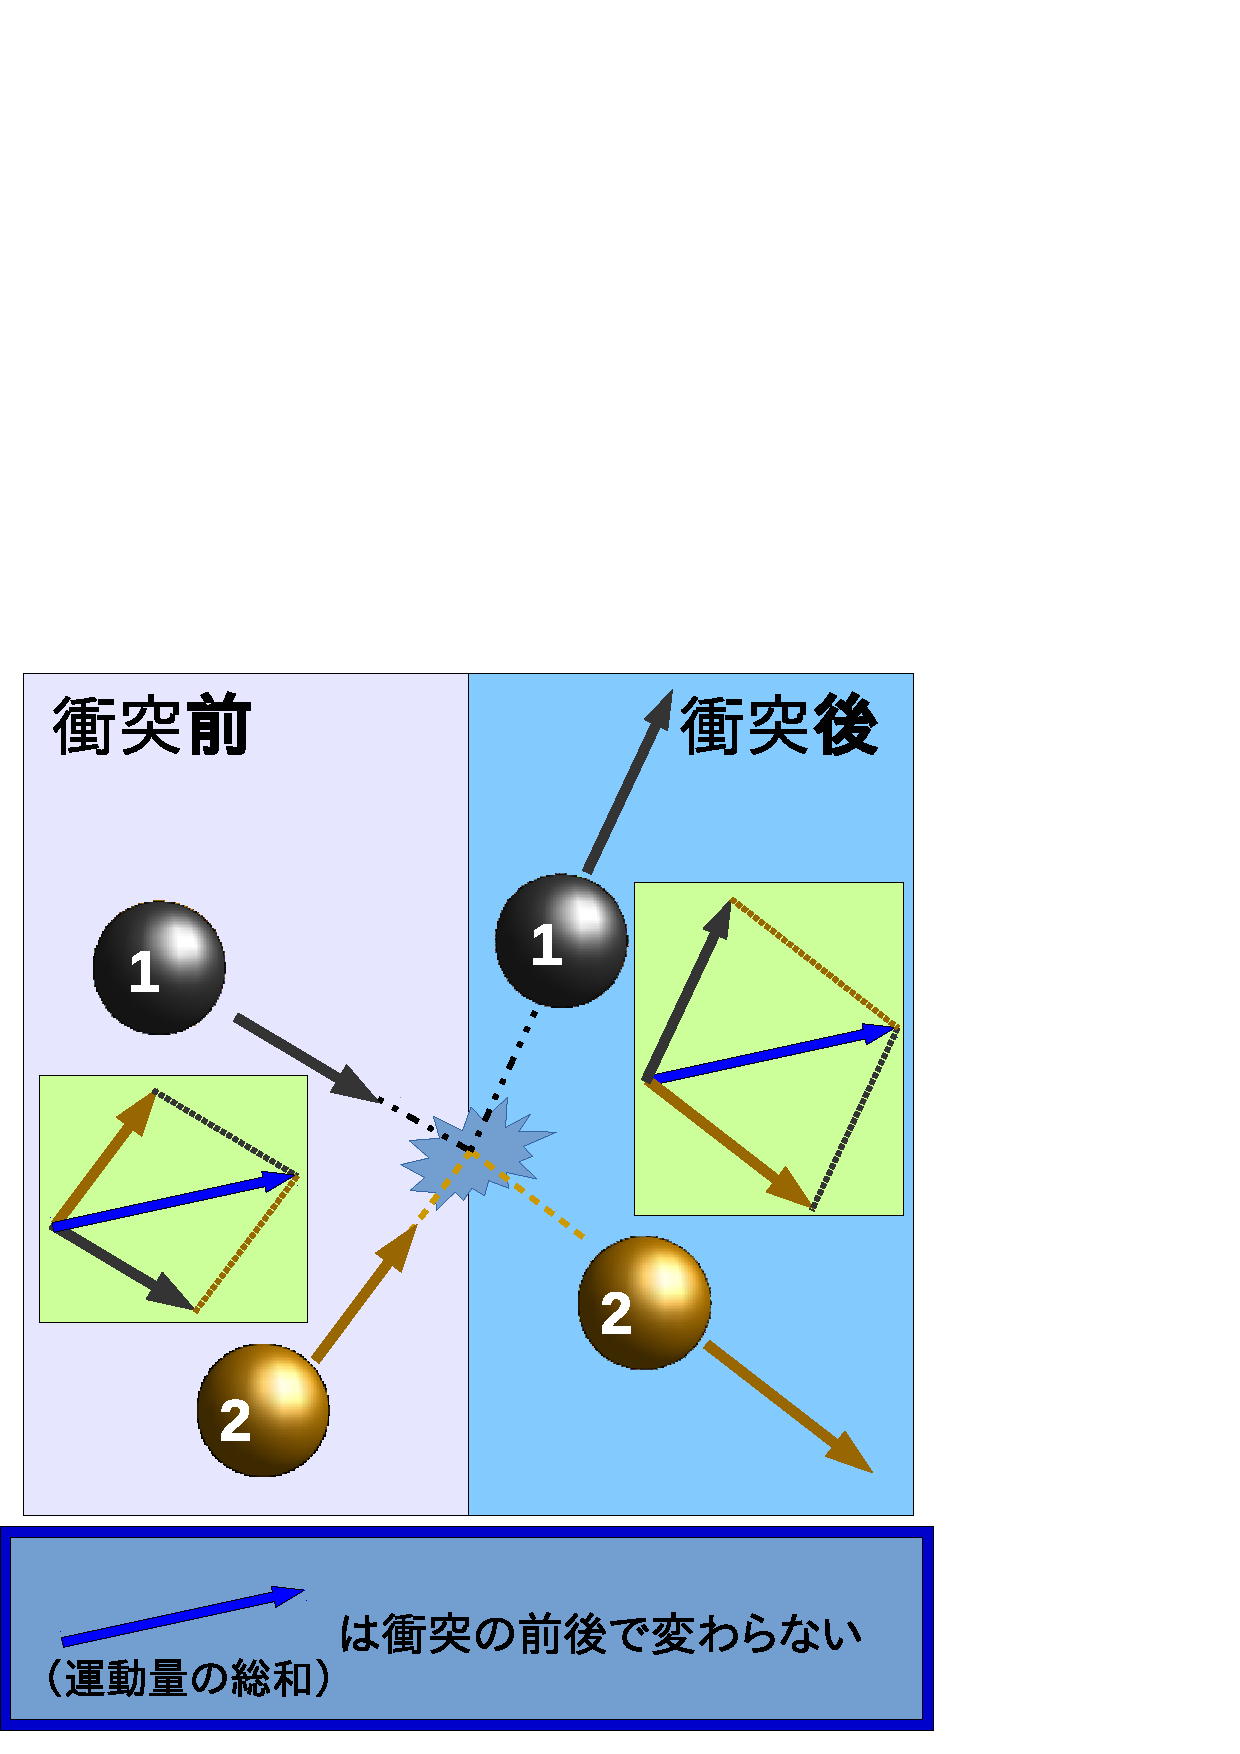
\includegraphics[keepaspectratio, width=6cm,height=8cm,clip]{P_hozonnsoku2.pdf}
                        \caption{運動量保存の法則}
                        \label{fig:Hozonasu}
                    \end{center}
                \end{figure}

            \begin{memo}{現象全体を見ることで,保存則が成立する}
                運動量保存の法則は,系の全ての物体について見渡すことで,成立している法則である.
                例えば,衝突に関係する物体全体の中の,一部の物体だけを見ているならば,
                この法則は成り立たない.1つの物体が運動量を増加させれば,
                別の物体は運動量を減少させるのである.
                この法則が意味していることは,この増加量と減少量の和が0になる ということである.
            \end{memo}

            \begin{memo}{運動方程式と運動量保存則}
                運動量保存の法則を次のように考えることもできる.すなわち,
                運動方程式$\df\textit{\textbf{P}}/\df t = \bF$ で,
                $\bF=0$ のとき,$\df\textit{\textbf{P}}/\df t =0$ である.
                従って,運動量保存の法則は運動方程式から導かれる.
            \end{memo}

            \begin{memo}{高校物理における運動量保存則}
                高校の物理学では,2つの物体の衝突を考えて,運動量保存の法則を説明した.
                より具体的な式で表現すれば,
                \begin{align}
                m_{a}\bv_{a\mbox{前}}+m_{b}\bv_{b\mbox{前}}=m_{a}\bv_{a\mbox{後}}+m_{b}\bv_{b\mbox{後}}
                \end{align}
                である.
            \end{memo}


%       %======================================================================
%       %  SubSection
%       %======================================================================
        \subsection{運動量の変化と力積}
            ある1つの物体の運動量が時間変化した場合について考える.物体が壁に当たって,
            運動方向を変化させる現象を想像するとよい.
            変化前と変化後の運動量をれぞれ,$\textit{\textbf{p}}_{\mbox{前}}$,
            $\textit{\textbf{p}}_{\mbox{後}}$ と書く.
            そして,このときの運動量の変化を $\textit{\textbf{I}}$ と書くことにすると,
                \begin{align}\label{7}
                    \textit{\textbf{I}} = \textit{\textbf{p}}_{\mbox{後}}-\textit{\textbf{p}}_{\mbox{前}}
                \end{align}
            である.

            ところで,物体が運動の方向を変化させたのだから,物体は力を受けたはずである.
            なぜなら,慣性の法則によると,
            物体に力が働かない限り,物体は等速直線運動をするからである.
            しかし,物体の運動量が変化したということは
            運動量の定義 $\textit{\textbf{p}} := m_{\mathrm{i}} \bv$ から,
            速度が変化したことになる.
            すなわち,加速度を生じたわけであり,力が加わったと解釈できる
                \footnote{
                    「加速度が生じること」と「力が加わること」は,運動方程式から,
                    同じことを意味すると言える.
                }.
            その力を $\bF$ とすると,運動方程式(\ref{6})から,
                \begin{align}
                    \frac{\df\textit{\textbf{p}}}{\df t} = \bF
                \end{align}
            をたてられる.この式の両辺を,衝突前の時間 $t_{\mbox{前}}$ から
            衝突後の時間 $t_{\mbox{後}}$ で定積分すると,
                \begin{align}\label{8}
                    \int_{t_{\mbox{前}}}^{t_{\mbox{後}}}\frac{\df\textit{\textbf{p}}}{\df t} \df t
                    &= \int_{t_{\mbox{前}}}^{t_{\mbox{後}}}\bF \df t \notag \\
                    \Leftrightarrow \int_{t_{\mbox{前}}}^{t_{\mbox{後}}}\df\textit{\textbf{p}}
                    &= \int_{t_{\mbox{前}}}^{t_{\mbox{後}}}\bF \df t \notag \\
                    \Leftrightarrow \textit{\textbf{p}}(t_{\mbox{前}})-\textit{\textbf{p}}(t_{\mbox{後}})
                    &= \int_{t_{\mbox{後}}}^{t_{\mbox{前}}}\bF \df t
                \end{align}
            となる.この式の左辺は,$\textit{\textbf{p}}_{\mbox{後}}-\textit{\textbf{p}}_{\mbox{前}}$ と
            全く同じことであるので,
            式(\ref{7})と式(\ref{8})を見比べると,
                \begin{align}
                    \textit{\textbf{I}} = \int_{t_{\mbox{前}}}^{t_{\mbox{後}}}\bF \df t
                \end{align}
            の関係を得る.この $\textit{\textbf{I}}$ のことを,\textbf{力積} という.
            つまり,運動量変化は力積 $\textit{\textbf{I}} =\int_{t_{\mbox{前}}}^{t_{\mbox{後}}}\bF \df t$
            によって生じたと考えられる.


%   %==========================================================================
%   %  Section
%   %==========================================================================
    \section{角運動量保存の法則}
        \begin{mycomment}
            回転している物体に共通する性質はあるだろうか.回転する物体として
            よく例に上がるのがコマである.また,車輪の例もよく見かける.
            回転するコマが倒れずに回転を続けられる理由や,走行中の自転車が
            安定している理由に,これから説明する角運動量保存の法則が絡んでいる.
        \end{mycomment}

%       %======================================================================
%       %  SubSection
%       %======================================================================
        \subsection{角運動}
            物体が一直線上を運動していても,ある固定された点からその物体の運動を眺めると,
            その点を中心として回転しているように見える.
            例えば,車が走っているのを見るとき,その車を1つの決まった場所から目で追うためには,
            首(あるいは目)を回転させる必要がある.
            このような回転運動のことを \textbf{角運動} という.
            (回転を表すのに角度を用いるからだろうか?)このような状況を思い浮かべつつ,
            角運動について考える.
            角運運動量を記述するには,ベクトルの \textbf{外積} の知識が必要である.

        \subsection{てこの原理}
            物体の回転の最も基本的な原理は,\textbf{てこの原理} である.
            そのままでは簡単には持ち上げられない程,重い物体があるとしよう.
            この物体を持ち上げたいとき,てこの原理が役に立つ.
            もはや,説明するまでもないだろう.図\ref{fig:teko_no_genri1}を見れば,
            分かるはずである.直接的に力を加えている部分を \textbf{力点},
            棒の回転の支えになっている点を \textbf{支点},重い物体に力がかかっている
            点を \textbf{作用点} という.
                    \begin{figure}[hbt]
                        \begin{center}
                            \includegraphicssqmid{teko_no_genri1.pdf}
                            \caption{てこの原理}
                            \label{fig:teko_no_genri1}
                        \end{center}
                    \end{figure}

            てこの原理は,重い物体を小さな力で持ち上げることを,可能にする.
            てこの原理を数式で表現してみよう.力点にかかる力を $F$ とし,
            持ち上げたい物体にかかる力(重力)を $W$ とする.
            てこの原理を使わずに,物体を持ち上げようとしても,
            加える力よりも物体の方が重く,すなわち
                \begin{equation*}
                    F < W
                \end{equation*}
            となるので,物体を持ち上げられない.

            てこの原理を使うと,上式が成り立っていても,物体を持ち上げることができる.
            支点と力点との距離を $l_{1}$,支点と作用点との距離を $l_{2}$ としよう.
            このとき,物体が持ち上がったとすると,てこの原理は
                \begin{align}
                    Fl_{1} > Wl_{2}
                \end{align}
            のように表現される.この式が成立するときに,物体を持ち上げられるの
            物体の重さ $W$ は一定であり,力 $F$ には限界値があることから,
            自由に動かせるのは ${l}_{1}$, ${l}_{2}$ しかない.
            支点から力点までの距離(${l}_{1}$)を長くし,
            支点から作用点までの距離(${l}_{2}$)を短くすることで,
            より小さい力で物体を持ち上げることが可能になる.

        \subsection{釣り合いの式}
            てこの原理の式の不等号を等号に置き換えた式を,釣り合いの式という.
                \begin{align}
                    {F}_{1}{l}_{1} = {F}_{2}{l}_{2}.
                \end{align}
            ${F}_{1}$ を物体の重さによってかかる力とし(力点),${F}_{2}$ を棒が傾かないように支える力とする(作用点).
            ${l}_{1}$ は支点と力点との距離で,${l}_{2}$ は支点と作用点との距離である.
                    \begin{figure}[hbt]
                        \begin{center}
                            \includegraphicslarge{TekonoGenri111.pdf}
                            \caption{釣り合い}
                            \label{fig:TekonoGenri111}
                        \end{center}
                    \end{figure}

%       %======================================================================
%       %  SubSection
%       %======================================================================
        \subsection{物体の回転の表現 と ベクトルの外積}
            物体が回転しているということを表現するのに,
            ベクトルの \textbf{外積} という概念を導入する.
            ここでは,このベクトルの外積について考える.

            物体が回転するということは,その軌道は円であるから,
            回転には必ずこの軌道円の中心を通る“回転の軸”が存在する.この回転の軸は直線であることは
            当たり前であって,確認するまでもない.この軸を用いて,回転の方向を表現するのである.
            回転の方向をこの軸方向にとって,回転の強さを適当に定義すれば,
            その回転の特徴を表現できる.さて,以下では回転の具体的な表現の仕方について
            考えていくことにしたいと思う.

            まず,回転の方向の決定方法である.これには回転の軸を用いることは先ほど書いたところである.
            その
            方向には正方向と負方向の2つがあるが,
            その取り決めは次の約束に従うものとされる.すなわち,回転の向きを
            \textbf{「
            速度の方向 $\bv$ の方向から,
            物体から軸へ垂線を下ろした向き($\textbf{\textit{k}}$ の方向)に
            右ねじを回して進向き」} と決めるのである.
            これを \textbf{右ねじの法則} という.
            回転の強さについてはもう少し後で考えるこにする.
                        \begin{figure}[hbt]
                            \begin{center}
                                \includegraphicssqmid{gaiseki1new.pdf}
                                \caption{物体の回転}
                                \label{fig:gaiseki1new}
                            \end{center}
                        \end{figure}

            右ねじの法則によって方向を定義されたベクトルを $\bL$ と書くことにする.
            これを,
            \begin{align}
            \bL=\textbf{\textit{k}} \times \bv
            \end{align}
            のように表現する.この式の解釈の仕方は,
            「ベクトル $\textbf{\textit{k}}$ をベクトル $\bv$ 方向へ右ねじ回して進む
            向き」のベクトルと読む.

            しかし,向きを設定したのではまだ不十分である.この $\bL$ の大きさを考える必要がある.
            そこで,大きさの定義として,「物体の速度ベクトル $\bv$ と
            垂線ベクトル $\textbf{\textit{k}}$ のなす平行四辺形の面積」を
            用いる.このような,ベクトルの大きさの定義の理由については後回しにして,
            ここではそのようなものであると考えておいてもらいたい.式でこの定義を表現すれば,
            \begin{align}
                L:=\|\bL\|=\|\textbf{\textit{k}} \times \bv\|
                =\| \textbf{\textit{k}} \| \| \bv \| \sin\theta
            \end{align}
            である.

            さて,ベクトルの大きさの具体的な
            定義を見てもらったところで,
            次にこの定義の意味の説明である.

            覚え方は,内積を定義したときには $\cos$ 関数を
            用いて定義したことと比べると,今回は
            この部分は $\sin$ 関数となっていることに注意すればよい
            ということだろうか.

            大体,物体の回転をベクトルを用いて表現すると
            以上のような感じだが,しかしこれでは感覚的過ぎる.
            そこで,この物体の回転を,ベクトルの成分を通して
            もう少し詳しく考えていくことにしたい.

%       %======================================================================
%       %  SubSection
%       %======================================================================
        \subsection{角運動量}
                \begin{figure}[hbt]
                    \begin{center}
                        \includegraphicssqmid{kaku_unndouryou2.pdf}
                        \label{fig:kaku_unndouryou2}
                        \caption{(a) 直線運動}
                    \end{center}
                \end{figure}
                \begin{figure}[hbt]
                    \begin{center}
                        \includegraphicssqmid{kaku_unndouryou1.pdf}
                        \label{fig:kaku_unndouryou1}
                        \caption{(b) 回転運動}
                    \end{center}
                \end{figure}

                物体が位置 $\br$ において,運動量 $\textit{\textbf{p}}$ をもっているとき,
                            \begin{align}
                            \bL
                            := \br \times \textit{\textbf{p}}
                            \end{align}
                で定義される $\bL$ を原点の周りの \textbf{角運動量} という.
                物体の角運動量 $\bL$ が0でない値をとるとき,その物体は回転運動
                をしていると言える.

%       %======================================================================
%       %  SubSection
%       %======================================================================
        \subsection{角運動の方程式}
                回転運動している物体の運動方程式を考えてみよう.

                角運動量 $\bL$ を時間微分すると,
                    \begin{align}\label{9}
                        \frac{\df\bL}{\df t}
                        = \frac{\df\br}{\df t} \times \textit{\textbf{p}}
                        +\br \times \frac{\df\textit{\textbf{p}}}{\df t}
                    \end{align}
                となる.ここで,式(\ref{9})の第1項の運動量 $\textit{\textbf{p}}$ は
                    \begin{align}
                        \textit{\textbf{p}} = m\bv=m\frac{\df\br}{\df t}
                    \end{align}
                である.これを用いて,
                    \begin{align}\label{9_1}
                        \frac{\df\bL}{\df t}
                        = \frac{\df\br}{\df t} \times m\frac{\df\br}{\df t}
                        +\br \times \frac{\df\textit{\textbf{p}}}{\df t}
                    \end{align}
                となるが,ベクトルの外積の性質
                (任意のベクトル $\bA$ に対して $\bA \times \bA=0$ が成り立つ)
                を考慮すると,
                    \begin{align}
                        \frac{\df\br}{\df t} \times m\frac{\df\br}{\df t}
                        =m\left( \frac{\df\br}{\df t} \times \frac{\df\br}{\df t} \right)=0
                    \end{align}
                となってしまうので,式(\ref{9_1})の第1項は 0 にってしまい,結局,
                    \begin{align}
                        \frac{\df\bL}{\df t} = \br \times \frac{\df\textit{\textbf{p}}}{\df t}
                    \end{align}
                と計算される.さらに,運動量を用いた運動方程式(\ref{6})の関係から,
                    \begin{align}\label{10}
                        \frac{\df\bL}{\df t} = \br \times \bF
                    \end{align}
                を得る.ここで,原点の周りの \textbf{力のモーメント} $\bN$を
                    \begin{align}\label{12}
                        \bN := \br \times \bF
                    \end{align}
                と定義すると,式(\ref{10})は
                    \begin{align}\label{11}
                        \bN = \frac{\df\bL}{\df t}
                    \end{align}
                と書ける.式(\ref{11})は,運動量を用いた運動方程式(\ref{6})と同じ形の式になっている.
                ($\bN$ → $\bF$,
                $\bL$ → $\textit{\textbf{p}}$ とするとわかる.)
                従って,式(\ref{11})は角運動についての運動方程式であると言える.
                力のモーメント $\bN$ は,角運動を引き起こす力である.
                すなわち,$\bN$ は回転運動を引き起こす力であると言える.
                このように回転力を起こす $\bN$ は \textbf{トルク} ともよばれる.

%       %======================================================================
%       %  SubSection
%       %=====================================================================
        \subsection{角運動量保存則}
                運動量保存則を考えたときに,
                「外部から力 $\bF$ が加わらない限り,全物体の運動量の総和は一定である」
                ということを確認した.
                角運動量についても同様な法則が成り立っていて,これを \textbf{角運動量保存の法則} という.
                または略して,\textbf{角運動量保存則} という.
                では,角運動量保存則 を式で表すことを考える.外力が働かないことから,$\bF=0$ であって,
                これを力のモーメントの定義式(\ref{12})に代入することで,
                $\bN := \br \times 0 =0$ を得る.よって,
                この $\bN=0$ を角運動についての運動方程式(\ref{11})に代入して,
                \begin{equation*}
                    \frac{\df\bL}{\df t} = 0
                \end{equation*}
                となる.この式は,外力が働かなければ,角運動量の時間変化がないことを示している.
                つまり,時間によらずに一定値をとることを意味する.従って,式(\ref{13})
                は角運動量保存則を表現した式であると言える.
                    \begin{myshadebox}{角運動量保存則}
                            位置ベクトル $\br$ にある物体に外力が働いていない場合($\bF=0$),
                            角運動量 $\bL$ は時間経過にかかわらず,一定に保たれる.
                            \begin{align}\label{13}
                                \frac{\df\bL}{\df t} = 0
                            \end{align}
                    \end{myshadebox}

                角運動量保存則を積分すれば,定ベクトルを得る.実際に確かめてみよう.
                角運動量保存則は 式(\ref{13})により $\df\bL/\df t = 0$ である.
                この角運動量 $\bL$ は $\bL
                := \br \times \textit{\textbf{p}}$ で定義される量であった.従って,
                角運動量保存則は
                    \begin{align}
                        \frac{\df \left(\br \times \textit{\textbf{p}}\right)}{\df t} = 0
                    \end{align}
                と表現しても同じことである.そして,両辺を時間で積分して,
                    \begin{align}
                        \int\left(\frac{\df \left(\br \times \textit{\textbf{p}}\right)}{\df t}\right) \df t = \bC
                    \end{align}
                ここに, $\bC$ は定ベクトルである.よって,
                    \begin{align}
                        \br \times \textit{\textbf{p}}=\bC
                    \end{align}
                を得る.この式は,位置 $\br$ が原点から遠くなるほど,運動量は小さくなることを意味している
                逆にいえば,原点に近いほど,運動量は大きくなるのである.

                例えば,スケーターの回転を考えてみる.この場合の座標原点は体の重心にとる.
                スケーターが自身の腕を大きく広げたときほど ゆっくりと回転している のは,手の位置 $\br$ が
                体の重心からより遠くなるためである.すなわち,これは $\br$ が
                大きくなることを意味する.しかし,特に外力が働かないので,(氷との摩擦は無視する)
                角運動量保存の法則 $\br \times \textit{\textbf{p}}=\bC$ が成立している.
                従って,運動量 $\textit{\textbf{p}}$ が小さくなるのである.
                というか,運動量を小さくすることで,角運動量保存則を満たそうとするのである.

                腕を縮めると回転が速くなるのは,この逆で,手の位置 $\br$ が
                体の重心に近づくからである.従って,角運動量保存則を満たすために
                運動量 $\textit{\textbf{p}}$ を大きくするのである.


%   %==========================================================================
%   %  Section
%   %==========================================================================
    \section{力学的エネルギー保存の法則}
%       %======================================================================
%       %  SubSection
%       %======================================================================
        \subsection{仕事}\label{shou_sigoto}
%       %======================================================================
%       %  SubsubSection
%       %======================================================================
        \subsubsection{1次元上の仕事}
                まず簡単に,一方向のみに限定して考える.その一方向を,$x$ 方向とする.
                さて,物体に外力 $F_{x}$ を加えて, $x$ 方向に $\Delta x$ だけ変位させたとしよう.
                物体の移動は,物体に与えた外力 $F_{x}$ とその変位の大きさ $\Delta x$ できまる.
                この移動は,物体が「仕事」をされたから,生じたものであると考える.仕事は,記号 $W$ で
                表され,次式よって定義される.
                    \begin{equation*}
                        W  :=  F_{x} \Delta x.
                    \end{equation*}
                単位は上の定義式から,[Nm] である.仕事の単位を表す記号は [J] が使われる.
                つまり,[J] = [Nm] である.単位については後で改めて,記述しよう.

                「仕事」という概念を導入することで,物体の移動を考えやすくなる.物体が
                移動したということは,物体に外力が働いて,変位したということであるが.
                その力の方向と変位の方向を考慮する必要がない場合,
                    \begin{equation*}
                        \mbox{物体は「仕事」} W \mbox{をされた.}
                    \end{equation*}
                あるいは,視点を変えて,
                    \begin{equation*}
                        \mbox{「仕事」} W \mbox{をした.}
                    \end{equation*}
                と表現できる
                    \footnote{
                        もう少し学習を進めると,「エネルギー」という概念が導入される.この「エネルギー」を
                        説明するために,「仕事」が使われるのであるが,実は後で記述するように,仕事と
                        エネルギーには,表と裏のような関係がある.「エネルギー」は,物理学で最も重要な
                        概念の1つである.
                    }.
                一方向だけで考えられるならば仕事の定義は上の式で十分である.

%       %======================================================================
%       %  SubsubSection
%       %======================================================================
        \subsubsection{3次元内の仕事}
                物体に力を加えたときの物体の変位の方向は,必ずしも,その力の方向であるとは限らない.
                変位も3次元を考えることができて,一方向だけではない.
                例えば,重い荷物を引っ張るとき,真横に力を加えるのではなく,少し上向きに引っ張ることが
                多い.このとき物体は地面から離れず,ただ地面に引きずられるという場合が起こり得る.
                そのとき,力が物体にした仕事は,その力の全てではなく,地面に対して平行な力の成分
                しか仕事をしていない.上向きの成分は,物体が上に上がっていないので,仕事はしていないのである.
                このような場合でも仕事を定義できるように導入されるのが,「なす角」である.
                ここでは,なす角を導入し,$\theta$ で表すことにしよう.
                「なす角」と聞いて,すぐにベクトルの内積が頭に浮かぶと思う.そうベクトルの内積を用いて,
                仕事を定義するのである.

                なす角 $\theta$ を導入すると,力を加えた方向と異なる向きに物体が移動したときにも,
                仕事を定義できるのである.
                    \begin{figure}[hbt]
                        \begin{center}
                            \includegraphicssqmid{sigoto_nasukaku.pdf}
                            \caption{力と仕事(3次元)}
                        \end{center}
                    \end{figure}

                少しかしこまった形で,なす角を導入しよう.
                物体が一定の力 $\bF$ で,\underline{直線距離} $\Delta \textit{\textbf{s}}$ だけ変位したとき,
                \textbf{仕事} $W$を次式で定義する.
                    \begin{align}
                        W:=\bF\cdot\Delta \textit{\textbf{s}}=F\Delta s \cos \theta
                    \end{align}
                ここに,$\theta$ は $F$ と $\Delta s$ の \textbf{なす角} (図\ref{fig:nasu}参照)である.
                    \begin{figure}[hbt]
                        \begin{center}
                            \includegraphicssqmid{nasu.pdf}
                            \caption{力 $\bF$ と変位 $\Delta\textit{\textbf{s}}$ のなす角 $\theta$ }
                            \label{fig:nasu}
                        \end{center}
                    \end{figure}


%       %======================================================================
%       %  SubsubSection
%       %======================================================================
        \subsubsection{仕事の単位}
                仕事の単位は[J]
                    \footnote{
                        ジュールと読む.仕事と熱量の関係を研究した物理学者Jouleの頭文字である.
                    }
                が用いられる.上の仕事の定義からわかるように,仕事の単位はSI単位系
                    \footnote{
                        SI単位系:基本単位として[m](メートル),[Kg](キログラム),[s](セコンド),[A](アンペア)
                        を用いる単位系のこと.\date 現在,SI単位系は国際標準となっている.
                        $\longrightarrow $昔はcgs単位系([cm](センチメートル),[g](グラム),[s])もよく使われていたみたいである.
                        古い教科書を見てみると,cgs単位系で書かれているもの多い.
                    }
                で,
                    \begin{align}\label{eq:Jule}
                        \mathrm{
                            [J]=[Nm]=[kgm^{2}/s^{2}]
                        }
                    \end{align}
                である.

%       %======================================================================
%       %  SubsubSection
%       %======================================================================
        \subsubsection{一般的な仕事の定義}
                次に,物体が 位置によって異なる力 $\bF(\br)$ で,
                \underline{曲線} $\br$ に沿って変位したときの仕事を考える.
                曲線の微小部分 $\df\br$ では力は一定と考えられる.
                よって,この微小部分 $\df\br$ における仕事は
                $\bF(\br) \cdot \df\br$ と書ける.
                すなわち,微小部分での仕事を積分すると,求める仕事 $W$ を得る.従って,位置 $\br_{A}$ か
                ら 位置 $\br_{B}$
                変位が曲線をとるときの仕事は
                    \begin{align}
                        W:=\int_{\br_{A}}^{\br_{B}}
                        \bF(\br) \cdot \df\br
                    \end{align}
                と定義できそうである.しかし,\textbf{これでは不十分である}.なぜなら,位置 $\br_{A}$ から
                位置 $\br_{B}$ までの曲線は無限に作れるからである.というのも
                そのような曲線によって,仕事が異なるからである.これは当たり前のだろう.
                曲線が変わってしまえば,物体の変位する“道のり”が長くなったり,短くなったりするのだから,
                当然,仕事もこの曲線によって異なると考えられる.
                そこで,位置 $\br_{A}$ から
                位置 $\br_{B}$ までの
                この曲線を指定する.それを \textbf{経路} という.位置 $\br_{A}$ から
                位置 $\br_{B}$ までの経路 $C$ に沿って,変位したときの仕事は,次のように書く.
                        \begin{myshadebox}{仕事の定義}
                            経路 $C$ に沿って物体を動かす際の仕事 $W$ を,次式で定義する.
                            \begin{align}
                                W=\int_{C}\bF(\br) \cdot \df\br.
                            \end{align}
                        \end{myshadebox}
                    \begin{figure}[hbt]
                            \begin{center}
                                \includegraphicssqmid{sensekibun_shukaisekibun_000.pdf}
                                \caption{点Aから点Bまで}
                                \label{fig:sigoto_keiro1}
                            \end{center}
                    \end{figure}


                特に,この\underline{経路が閉曲線である場合},
                    \begin{align}
                        W=\oint_{C}\bF(\br) \cdot \df\br
                    \end{align}
                と書かれることがある.\ref{subsec:hozonryoku_to_shukaisekibun} 節も参照.
                    \begin{figure}[hbt]
                            \begin{center}
                                \includegraphicssqmid{sensekibun_shukaisekibun_003.pdf}
                                \caption{始点と終点が同じ}
                                \label{fig:keiro_loop}
                            \end{center}
                    \end{figure}

                \begin{memo}{注意}
                    もう一度書いておくが,仕事を計算するときは,最初に経路を指定することが必要である.
                    今までの話だと,仕事が経路によって異なってしまうのだから,
                    このような定義では十分でないと思われるかもしれないが,
                    ここで仕事という概念を定義したのは,
                    この仕事が経路によらないような力を導入したいためである.
                    そのような力の例として,最も簡単な例に,地表付近の
                    物体が受ける力 $m\textit{\textbf{g}}$ がある.
                    どのように示されるかは以下で考えることである.
                \end{memo}

%       %======================================================================
%       %  SubSection
%       %======================================================================
        \subsection{エネルギーについて}
%           %==================================================================
%           %  SubsubSection
%           %==================================================================
            \subsubsection{エネルギー}
                物体が外部から仕事を受けたとき,その物体は \textbf{エネルギー} を
                与えられたという.例えば,人間が物体を高さ $h$ だけ上にあげれば,
                物体は人間による外力から仕事されたことになり,
                従ってエネルギーを外力から与えられたということになる.

                数式っぽく表現すれば以下のようなるだろう.すなわち,
                    \begin{center}
                        『外力が物体に仕事をする=物体は外力を受けることにより,エネルギーを与えられる.』
                    \end{center}
                つまり,「エネルギーをもつ」ということは「仕事ができる状態にある」
                ということと同じである.
                従って,\textbf{仕事とエネルギーは同じ単位をもつ}.
                エネルギーと仕事の関係は視点の違いこそあるけれど,
                同等なものであると言える.「仕事」という時は外力を主眼と考えるときであり,
                「エネルギー」という時には物体を主眼として考えていると言える.
                    \begin{figure}[hbt]
                        \begin{center}
                            \includegraphicssqmid{ENERGY_1.pdf}
                            \caption{仕事とエネルギー}
                            \label{fig:ENERGY_1}
                        \end{center}
                    \end{figure}

                                仕事をする側はエネルギーが減り,仕事をされる側はエネルギーが増えるのである.
                                これを式で表現してみよう.摩擦などの外的要因はない理想状態で考える.

                                まず,仕事をする側に着目する.$W$ だけ仕事をした場合,
                                もともと持っていたエネルギーを $E_{a0}$ とすると
                                        \footnote{
                                                $E_{a0}$ の $a$ は仕事"する"側で,能動を意味する英単語 active の頭文字を使った.
                                                0は仕事する前を示すものとし,1を仕事した後を示すものとして使う.
                                                仕事"される"側は,受動を意味する英単語 passive の $p$ を使う($E_{p0}$,$E_{p1}$).
                                        },
                                仕事した後のエネルギー $E_{a1}$ は,
                                        \begin{equation*}
                                                E_{a1} = E_{a0}-W.
                                        \end{equation*}

                                一方で,仕事をされた方は $W$ だけのエネルギーが入ってくる.
                                仕事される側のもともと持っていたエネルギーを $E_{p}$ とすると,
                                仕事をされた後のエネルギー $E_{p1}$ は,
                                        \begin{equation*}
                                                E_{p1} = E_{p0}+W.
                                        \end{equation*}
                                つまり,
                                        \begin{align}
                                                E_{a1} + E_{p1} &= (E_{a0}-W) + (E_{p0}+W)  \notag \\
                                                                &= E_{a0} + E_{p0}
                                        \end{align}
                                と計算され,仕事する前後では,"する側" と "される側" の全系で考えた場合,
                                全体的なエネルギーの変化はないことがわかる.実験的にも,摩擦などを極力小さくした場合,
                                上式に反した結果はない.こうなると,これを逆手に取り,
                                「物体の運動状態が変化しても,総エネルギーは変化しない」という仮説を立てたくなる.
                                実際,\textbf{エネルギー保存の法則} として,この仮説は物理法則の重要な1つに格上げされる.

                                ただ,エネルギーと言っても,運動やポテンシャルに関するもの,熱に関するもの,電磁気に関するものなどと,
                                様々な形態がある.すごいことに,どんな形態でも,エネルギー保存の法則が成立することが確かめられている
                                (実験事実).この法則が各エネルギー形態でどう表現されるかは非常に興味のあることである.
                                以下では,特に力学に関するエネルギー(運動エネルギーと位置エネルギー)を中心に,エネルギーという
                                概念について少し詳しく勉強していくことにしよう.

%           %==================================================================
%           %  SubsubSection
%           %==================================================================
            \subsubsection{エネルギーの種類}
                先にも書いたが,物体のもつエネルギーには,様々な形態がある.例えば,運動エネルギー,
                ポテンシャル$\cdot$エネルギー,熱エネルギー,電磁気的エネルギー 等がある.これらは全てエネルギーである.

                なぜこういうことが言えるかというと,一言で言うと,そう考えると意味のある理論が作れるからということになる.
                最初は,物体の運動に関すること,熱に関すること,電気に関すること,磁気に関すること,と言ったように,
                物理分野の別々の側面から現象が観測されていて,そもそもエネルギーという抽象的な概念はなかった.
                各分野の発展に伴い,それらに共通部分が見出されてくることも多い.その1つに,エネルギーがある.
                各分野がエネルギーという概念により有機的につながることがわかったのである.
                しかし,エネルギーとは人が様々な物理現象の研究から炙りだした抽象概念であり,"エネルギーそのもの" というものは
                ない.エネルギーを見るには,電気や熱などの具体的な現象を見るしかない.

                なので,勉強する際も,様々に現れる具体的なエネルギー形態を一つずつ確かめながら,
                エネルギーという概念の把握に努めたい.
                抽象的なエネルギーとはこうだ,と定義してから各分野でエネルギーがどう現れるかを
                議論したいところだが,まず現象を知らないとエネルギーについてのイメージを持ちようがないのだ.
                面倒だが,具体例を逐一見ていくしかない.

                どの形態のエネルギーも等しく重要な概念であり,全てのエネルギー形態について調べる必要があるが,
                以下ではその最も基本であるとされる,運動エネルギーと位置エネルギーについて考える.

%           %==================================================================
%           %  SubsubSection
%           %==================================================================
            \subsubsection{「エネルギー」のイメージ}
                                とはいっても,何のイメージもなしにエネルギーについて勉強するのはつらい.ジレンマだ.
                                ここでは,その概念の重要さについて記述することで,学習意欲を少しでも高めたい.

                エネルギーの概念は簡単につかめるものではない.少しもどかしいかもしれないが,とりあえずはエ
                ネルギーとはこんなものだと思って,先に進んでしまうことである.その進んだ先で,違った形の色
                々なエネルギーを見ることになるだろう.これらの色々な形のエネルギーをみて,初めて,エネルギ
                ーという感覚がつかめていくことだろう.ここは先人の知識を信じて先に進もう.エネルギーという
                概念はもうとっくに定着しているものであり,覆ることはないのだから…

                いや,むしろエネルギーそのものを,具体的に想像することはできない.エネルギーを知っていると
                いうかもしれないが,それは熱だとか電気だとか,何か物理的な現象となって生じているので,その
                ものを見てはいない.ではなぜ,エネルギーという概念が生まれたのだろうか.
                物理学には \textbf{保存則} というキーワードがある.保存則とは,例えば,ある現象の前後で変化
                しない量が存在するとき,この量は保存するといい,この法則のことを保存則という.
                また \textbf{保存量} とは,時間的に増えたり減ったりしない,何か本質的な量のことをいう.昔の
                人々は,物理法則を考えるにあたって,保存量を見つけ出すことにも力を注いでいた.この保存量の
                一つがエネルギーである.つまり,エネルギーは保存量として導入されたものである.

                実をいうと,エネルギーが保存することを実験で確かめる必要があるのだが,実験には誤差がつきも
                のであるので,厳密にはわからない.それにもかかわらず,エネルギーは保存すると言えるのは,そ
                の他の実験との矛盾がなく,むしろエネルギーが保存することでいろいろな現象を説明することがで
                きるからである.


%       %======================================================================
%       %  SubSection
%       %======================================================================
            \subsection{ポテンシャル$\cdot$エネルギー}
%           %==================================================================
%           %  SubsubSection
%           %==================================================================
            \subsubsection{高さ(位置)によるエネルギーの違い}
                地表面を位置の基準に取る.$z$ 座標を鉛直上向きを正にとる.
                質量 $m$ の物体を地表面から,高さ $h$ のところまで,
                垂直にではなく,クネクネ と曲がった経路 $C$ でもち上げられたときの仕事を考える.
                図\ref{fig:PE_fig}を参照.
                    \begin{figure}[hbt]
                        \begin{center}
                            \includegraphicssqmid{PE_fig.pdf}
                            \caption{物体の移動のある瞬間}
                            \label{fig:PE_fig}
                        \end{center}
                    \end{figure}

                このとき,持ち上げるのに要する力 $\bF(\br)$ は必ずしも鉛直上向きではない.
                力に負の符号をつけたのは,鉛直下向きを正とした
                ことによる.鉛直下向きの重力に逆らって 物体を持ち上げるのだから,
                負の符号がつくのである.
                この力を鉛直な成分 $\bF
                (\br)_{\perp}$
                と地面に水平な成分 $\bF
                (\br)_{\parallel}$ に分解する.
                    \begin{align}
                        \bF(\br)=\bF_{\perp}(\br)
                        +\bF_{\parallel}(\br)
                    \end{align}
                この力を経路に沿って線積分する.
                    \begin{align}
                        W &= \int_{C}\left(\bF_{\perp}(\br)   + \bF_{\parallel}(\br) \right) \cdot \df\br \notag \\
                          &= \int\bF_{\perp}(\br)\cdot \df\br + \int\bF_{\parallel}(\br) \cdot \df\br
                    \end{align}
                地表付近における,物体の地球から受ける力は,$m\textit{\textbf{g}}$ である.
                これを上式に代入するのだが,
                重力加速度の向きは鉛直方向を向いているので,水平方向との内積は0になる.(
                力の 鉛直成分 と 変位の水平移動方向 のなす角は
                $\frac{\pi}{2}$である.)従って,第1項のみが残って,
                    \begin{align}
                        W=-\int m\textit{\textbf{g}}\cdot \df\br
                    \end{align}
                となる.さらに,外力の鉛直方向と重力加速度とのなす角は $\pi$ であることを考慮し,
                $\textit{\textbf{g}} \cdot \df\br=g\df r \cos \pi=-g\df r$ の関係から,
                    \begin{align}
                        W=-mg\int \df r.
                    \end{align}
                内積計算を行ったので,ベクトル演算が消え,スカラー積となったことに注意.
                ここで,垂直方向は0になっていたために,上の $dr$ は鉛直成分を考えばよく, $h=\int \df r$ であるので,
                    \begin{align}
                        W=-mgh
                    \end{align}
                を得る
                    \footnote{
                        意味を強調するのであれば,$W=m(-g)h$ と書いたほうがよい.
                        質量 $m$ は常に正であるし,高さ $h$ は地表から空へと向かう
                        向きを正としているから,この場合は正の値をとるはずである.重力加速度 $\bg$ の向きは逆向きの
                        外力 $\bF_{\mbox{外力}} = -m\bg$ を加えることにより,
                        距離(ここでは高さ)$h$ だけ移動させ($W=m(-g)h$ の仕事をしたことになる),
                        物体にポテンシャル$\cdot$エネルギー $U=m(-g)h$ を与えたのだ.与えたエネルギーは仕事と
                        等しく,$W=U$ である(ポテンシャル$\cdot$エネルギーの定義).
                        物体に仕事 $W$ を与えたことにより,物体にエネルギー $U$ が溜められたと
                        いうイメージだ.見方を変えれば $W-U=0$ で,物体に与えた仕事 $W$ と
                        溜まったエネルギー $U$ の正味の和は0であり,物体のエネルギーは勝手に
                        湧きだしたものではなく,外力のみによって与えられたと捉えることもできる.
                    }.
                この計算結果から,いかなる経路でも,物体を高さ $h$ まで持ち上げるのに
                必要な仕事は,$W=-mgh$ であることがわかる.
                なぜなら,力がどんな方向に向いていようが,
                地面に垂直な成分 と 地面に平行な成分 に分割することができ,地面に平行な成分は
                全く仕事には関与せずにいるからである.
                力の 鉛直成分 と 変位の水平移動方向 の内積がいつも 0 であることからこのことがいえる.
                力が位置に依存するにしても,高さが決まってしまえば,上の計算からどんな場合でも
                 $-mgh$ の結果を得てしまうことは明らかである.

%           %==================================================================
%           %  SubsubSection
%           %==================================================================
            \subsubsection{エネルギーの値が負であるのはなぜか}
                ポテンシャル$\cdot$エネルギーには負の符号が付いている.
                これは,負の値をもつエネルギーを意味するのだろうか.
                答えは否.エネルギーが負の値を取るなんて考えられないのだから
                    \footnote{
                        ただし,量子力学を学習していくと,量子力学と特殊相対性理論
                        とを統一すると(最初にディラックが成功した),負の値をとる
                        エネルギーが生じることを発見した.実際に,負のエネルギーを
                        認めると,陽電子の存在が予言され,これは実際に実験的に確か
                        められている(ディラックはノーベル賞を得ている).

                        ここで言う負の符号と,ディラックの負値のエネルギーとは全く
                        概念が異なる.負値のエネルギーについては,相対論的量子力学
                        を学ぶ際に,出会うことになる.

                        まあ,細かいことは後回しにして,話を先に進めよう.
                    }.
                では,この負の符号はどういうことかというと,単に重力加速度 $g$ の
                向きの定義によるものである.
                物体を持ち上げるには,重力加速度に逆らって仕事を加えないと
                ならないが,重力加速度の向きを鉛直下向きを正方向としたので,
                仕事する方向が負になってしまうのである.

                高さ $h$ に位置する物体は,仕事 $W=-mgh$ を受けて,地上から上がったのである.
                重力に逆らって,高さ $h$ までもち上げたのだから,
                重力は物体を元も位置(地表)に戻そうとする.
                従って,この物体は,$-mgh$ の仕事をし得る状態にある.
                $-mgh$を,地表付近の重力の \textbf{ポテンシャル$\cdot$エネルギー} という.
                または \textbf{位置エネルギー} ともよばれる.
                地表から高さ $h$ にある物体は「潜在的に」$-mgh$ の仕事をし得ると考えるのである
                    \footnote{
                        「負の仕事をし得る」という表現は何か不可解であるならば,「正の仕事を\textbf{される}」
                        と表現しても同じことである.これは単に言葉による表現の仕方の違いであって,
                        その内容は全く同等なものである.
                    }.

%           %==================================================================
%           %  SubsubSection
%           %==================================================================
            \subsubsection{ポテンシャル$\cdot$エネルギーの定義}
                改めて,地表付近における重力のポテンシャル$\cdot$エネルギー $U$ を定義する.
                    \begin{align}
                        U := -mgh
                    \end{align}
                ここに,$m$ は質量であり,$g$ は重力加速度であり,$h$ は高さである.
                    \begin{figure}[hbt]
                        \begin{center}
                            \includegraphicssqmlrg{itienerugi.pdf}
                            \caption{高さ $h$ でのポテンシャル$\cdot$エネルギー}
                            \label{fig:itienerugi}
                        \end{center}
                    \end{figure}

%           %==================================================================
%           %  SubsubSection
%           %==================================================================
            \subsubsection{一般的なポテンシャルエネルギー}
                実は今まではポテンシャル$\cdot$エネルギーとして
                地表付近の重力によるものを想定してきたが,
                ポテンシャル$\cdot$エネルギーとはこれだけではなく,
                電気的なポテンシャル$\cdot$エネルギーというものも考えられる.
                これを \textbf{電位} というが,詳細は電磁気学の部分で
                確認することとする.とりあえず,ここでは,そのような概念もあるのだ
                と思ってくれればよい.ここで言いたかったことは,
                ポテンシャルが位置エネルギーだろうが電位だろうが,
                エネルギー保存の法則を満たすということである.エネルギー保存の法則を
                もっと一般的に捉えられるということを理解してほしい.

%       %======================================================================
%       %  SubSection
%       %======================================================================
        \subsection{運動エネルギー}
            \begin{mycomment}
                運動エネルギーをいきなり定義しても
                わけがわからないと思うので,とりあえず感覚的に理解できるような形で
                説明する.
            \end{mycomment}

%           %==================================================================
%           %  SubsubSection
%           %==================================================================
            \subsubsection{物体を高いところから落とすと$\cdots$}
                前の項目において,地表付近のポテンシャル$\cdot$エネルギーは $-mgh$ であることが分かった.
                ここで,$m$ は質量を表し,$h$は高さを表す.
                今,高さ $h$ に存在する物体が静に落下し(初速度は 0),
                高さ $h-\Delta h(<h)$ に変化したとする.
                このときの位置エネルギーは $-mg\left(h-\Delta h\right)$ である.
                高さが $h$ から$h-\Delta h$に変化したことで,
                位置エネルギーがどれだけ変化したかを考えれば,$-mg\Delta h$ である.
                $-mg\Delta h$のエネルギーはどこにいってしまったのだろうか.
                実は,\textbf{運動エネルギー} に変わったのである.つまり\underline{速度をもった}のである.
                図\ref{fig:KE_fig}参照.
                    \begin{figure}[hbt]
                        \begin{center}
                            \includegraphicssqmlrg{rakka_k.pdf}
                            \caption{運動エネルギーの説明}
                            \label{fig:KE_fig}
                        \end{center}
                    \end{figure}

%           %==================================================================
%           %  SubsubSection
%           %==================================================================
            \subsubsection{位置エネルギーから運動エネルギーへ}
                以下では,この運動エネルギーについて考える.
                位置が変位して速度が生まれたのだから,位置と速度の関係式が使える.
                位置と速度の関係式は,
                    \begin{align}
                        2\textit{a}\left(\textit{r}-\textit{r}_{0}\right)
                        =\textit{v}^{2}-{\textit{v}_{0}}^{2}
                    \end{align}
                のように表現される.
                但し,ここでは鉛直方向を考えているので,大きさだけを考えている.
                この式に,今の条件
                (初速度 $\textit{v}_{0}=0$ ,初期位置$\textit{r}_{0}=h$
                ,重力加速度$\textit{a}=\textit{g}$ ,現在の位置$r=h-\Delta h$)
                を代入して,
                    \begin{align}
                        2\textit{g}\cdot\left(-\Delta h\right)
                        =\textit{v}^{2}
                    \end{align}
                となる.従って,
                    \begin{align}
                        \Delta h = -\frac{\textit{v}^{2}}{2g}
                    \end{align}
                を得る.これを位置エネルギーの変化量 $-mg\Delta h$ に代入すると,
                    \begin{align*}
                        -mg\Delta h =- mg\left(-\frac{\textit{v}^{2}}{2g}\right) = \frac{1}{2} m {\textit{v}^{2}}
                    \end{align*}
                すなわち,
                    \begin{align}
                        -mg\Delta h = \frac{1}{2} m {\textit{v}^{2}}
                    \end{align}
                を得る.
                これはつまり,
                            \textbf{
                            位置エネルギーの変化が鉛直下向きの速度をもつ 運動エネルギー に変換された
                            }ことを意味する.
                この量はポテンシャル$\cdot$エネルギーと等価な量である.

%           %==================================================================
%           %  SubsubSection
%           %==================================================================
            \subsubsection{運動エネルギーの定義}
                上の説明から,物体の持つポテンシャル$\cdot$エネルギーが,
                落下等の現象によって,速度に関するエネルギーに変換されることが
                わかった.落下によって,ポテンシャル$\cdot$エネルギーが失われ,
                速度に関するエネルギーに変わったので,この新しいエネルギーに
                名前を付けないとならない.

                そこで,運動エネルギー $T$ を定義する.
                    \begin{align}
                        T :=  \frac{1}{2} m {\textit{v}^{2}}
                    \end{align}

                ここで,このように定義した運動エネルギーは
                エネルギーの単位[J]をもつかどうかを確かめておく.
                質量の単位は[kg],速さの単位は$\mathrm{[m/s]}$であるから,
                    \begin{align}
                        \mathrm{ [kg\cdot (m/s)^{2}]} &= \mathrm{[kg\cdot m^{2}/s^{2}]      } \notag \\
                                                      &= \mathrm{[(kg\cdot m/s^{2})\cdot m] } \notag \\
                                                      &= \mathrm{[N\cdot m]=[J]             }
                    \end{align}
                となって,確かにエネルギーの単位をもつことがわかる.「エネルギーを得る」ということは
                仕事をされるということであり,エネルギーの単位は仕事の単位と等しい.
                つまり,エネルギーの単位も [J] である.確かに運動エネルギーの単位は[J]であるとが確かめられた.

%           %==================================================================
%           %  SubsubSection
%           %==================================================================
            \subsubsection{運動量と運動エネルギーの関係式}
                当たり前ではあるが,運動エネルギーについては,
                ここで定義したものしか存在しない.運動エネルギーが
                運動量を用いて $T=p^{2}/2m$ と書かれる
                こともあるだろうが,これは,$\textit{\textbf{p}}=m\bv$ の関係式を思い出せば,
                $T=mv^{2}/2$ 全く同じことを言っているとわかる(代入してみればよい).
                    \begin{align}
                        T=\frac{1}{2}mv^{2}=\frac{m}{2m}mv^{2}=\frac{(mv)^{2}}{2m}=\frac{p^{2}}{2m}.
                    \end{align}

                運動エネルギーは,運動量と速度のどちらでも表現可能だが,その違いは
                単に表記の違いだけであって,2種類の運動エネルギー存在するわけではない.


%       %======================================================================
%       %  SubSection
%       %======================================================================
        \subsection{力学的エネルギー保存の法則}
%           %==================================================================
%           %  SubsubSection
%           %==================================================================
            \subsubsection{高校生向けの説明}
                ポテンシャル$\cdot$エネルギー $U$ と運動エネルギー $T$ の和を \textbf{力学的エネルギー} という.
                力学的エネルギーを $E$ で表現する.
                    \begin{myshadebox}{力学的エネルギーの定義}
                        力学的エネルギー $E$ を,次式で定義する.
                        \begin{align}\label{eq:KE}
                        E := T + U
                        \end{align}
                    \end{myshadebox}


                このように定義された力学的エネルギーをもつ物体は,
                外力が働かない限り,
                保存する.
                「保存する」というのは「ある一定の値を保つ」ということである.
                このことを \textbf{力学的エネルギー保存の法則} という.
                力学的エネルギー保存の法則を表す式を導出する.そのために,もう一度,式(\ref{5})を使う.
                簡単のために,運動を一方向にかぎって考える.
                最初の状態(速度$v_{1}$,位置$h_{1}$)から,後の状態(速度$v_{2}$,位置$h_{2}$)に変化しとする.
                すると,
                    \begin{align}
                        2\textit{g}\left(\textit{h}_{2}-\textit{h}_{1}\right)
                        ={\textit{v}_{2}}^{2}-{\textit{v}_{1}}^{2}
                    \end{align}
                という式が立てられる.この式の両辺に,質量 $m$ を掛けて整理すると,
                    \begin{align}
                        2mg\left(\textit{h}_{2}-\textit{h}_{1}\right)
                        &= m{\textit{v}_{2}}^{2}-m{\textit{v}_{1}}^{2} \notag \\
                        \Leftrightarrow\quad 2mgh_{2}-2mgh_{1}
                        &= m{\textit{v}_{2}}^{2}-m{\textit{v}_{1}}^{2} \notag \\
                        \Leftrightarrow\quad mgh_{2}-mgh_{1}
                        &= \frac{1}{2}m{\textit{v}_{2}}^{2}-\frac{1}{2}m{\textit{v}_{1}}^{2} \notag \\
                        \Leftrightarrow\quad \frac{1}{2}m{\textit{v}_{1}}^{2}-mgh_{1}
                        &= \frac{1}{2}m{\textit{v}_{2}}^{2} -mgh_{2}
                    \end{align}
                この式は,始めの状態の力学的エネルギーの和 と 後の状態の
                力学定エネルギーの和 が等しいことを意味している.すなわち,
                力学的エネルギーは,一定値を取り,力学的エネルギー保存の法則 が
                成立していることを確認できた.

%           %==================================================================
%           %  SubsubSection
%           %==================================================================
            \subsubsection{微分の知識を使う方法}
            \begin{mysmallsec}{理論的な導き方とは}
                もっと高度
                    \footnote{
                        「高度」という単語に深い意味はない.ただ単に,
                        格好良くとか,そういった感じのニュアンスで使っただけ.
                    }
                に導出してみよう.
                力学的エネルギー保存の法則は,ニュートンの運動方程式から数学的に
                導ける.
                更に,この導出の段階で,ポテンシャル$\cdot$エネルギーと
                運動エネルギーが現れてくる
                    \footnote{
                        力学的エネルギー保存の法則が導かられるのだから,
                        当然として,その過程で,ポテンシャル$\cdot$エネルギー
                        と運動エネルギーが現れてこないとおかしい.
                    }.
            \end{mysmallsec}

            \begin{mysmallsec}{方針}
                仕事とエネルギーの関係式を導くのが目標.先に結論を軽てしまうと,
                物体に一定期間の仕事を与えると,その物体にはエネルギーが蓄積する
                ということである.なので,式変形方針としては,仕事の定義である,
                力と移動変位の積($\bF\cdot\br$)を時間$t$で積分する.ニュートンの
                運動方程式をもとにする.
            \end{mysmallsec}

            \begin{mysmallsec}{導出}
                ニュートンの運動方程式 $m_{\rm{i}}(\df^{2}\br/\df t^{2}) = \bF$
                の両辺に,$\df\br$ を掛ける
                    \footnote{
                        要するに,「仕事の形を作っていこう」ということである.
                    }.
                    \begin{align}\label{eq:energy_and_work}
                        m\frac{\df^{2}\br}{\df t^{2}}\cdot \df\br
                    \end{align}
                左辺は仕事の定義そのものである.左辺がこのままだと意味不明なので,計算を進めてみよう
                    \footnote{
                        左辺が仕事だから,右辺も仕事と言っても間違いはないのだが,計算を進めると面白い
                        結果が得られる.統合で結ばれているので,仕事と同じ次元の物理量が導かれる.
                        先にも触れている通り,運動エネルギーとポテンシャル$\cdot$エネルギーがみえてくる.
                    }.

                次のように,右辺を移行しておく
                    \footnote{
                        そうすると,エネルギー保存則に近い形になるから.
                    }.
                    \begin{align}
                        m\frac{\df^{2}\br}{\df t^{2}}\cdot \df\br
                         &= \bF\cdot \df\br \notag \\
                        \Leftrightarrow m\frac{\df^{2}\br}{\df t^{2}}\cdot \df\br
                        -\bF\cdot \df\br &= 0
                    \end{align}

                まず,第1項について以下のような計算をする.
                    \begin{align*}
                        \frac{\df^{2}\br}{\df t^{2}}\cdot \df\br
                        =\frac{\df^{2}\br}{\df t^{2}}\cdot \frac{\df\br}{\df t}\df t
                        =\frac{\df }{\df t}\frac{\df\br}{\df t}\cdot \frac{\df\br}{\df t}\df t
                    \end{align*}
                計算が簡単になるように速度に置き換えて,
                        \begin{equation*}
                                \bv=\df\br/\df t
                        \end{equation*}
                とすれば,
                    \begin{align*}
                        \frac{\df^{2}\br}{\df t^{2}}\cdot \df\br
                        =\left(\frac{\df\bv}{\df t}\cdot \bv\right) \df t.
                    \end{align*}
                ここで,
                    \begin{align*}
                    \frac{\df\bv^{2}}{\df t}&=\bv\frac{\df\bv}{\df t}
                    +\frac{\df\bv}{\df t}\bv = 2\bv\frac{\df\bv}{\df t} \\
                    \Leftrightarrow \quad
                    \bv\frac{\df\bv}{\df t}&=\frac{1}{2}\frac{\df\bv^{2}}{\df t}\\
                    \Leftrightarrow \quad
                    \frac{\df^{2}\br}{\df t^{2}}\cdot \df\br&=
                    \left(\frac{1}{2}\frac{\df\bv^{2}}{\df t}\right) \df t\\
                    \therefore \quad
                    \frac{\df^{2}\br}{\df t^{2}}\cdot \df\br&=\df \left(\frac{1}{2}\bv^{2}\right).
                    \end{align*}
                以上より,速度の表記を元に戻せば,
                    \begin{align*}
                        \frac{\df^{2}\br}{\df t^{2}}\cdot \df\br=\df \left( \frac{1}{2}\left( \frac{\df\br}{\df t} \right)^{2} \right)
                    \end{align*}
                と計算でき,これを用いると,
                    \begin{align}\label{b}
                        m\,\df \left( \frac{1}{2}\left( \frac{\df\br}{\df t} \right)^{2} \right)
                        -\bF\cdot \df\br &= 0 \notag \\
                        \Leftrightarrow \quad m\int \df \left( \frac{1}{2}\left( \frac{\df\br}{\df t} \right)^{2} \right)
                        -\int \bF\cdot \df\br &= C \notag \\
                        \Leftrightarrow \quad\frac{m}{2}\left( \frac{\df\br}{\df t} \right)^{2}
                        -\int \bF\cdot \df\br &= C \notag \\
                        \Leftrightarrow \quad\frac{1}{2}mv^{2}
                        -\int \bF\cdot \df\br &= C.
                    \end{align}
                見慣れた形をした項が現れた.
            \end{mysmallsec}

            \begin{mysmallsec}{解釈}
                式\eqref{eq:energy_and_work}の右辺は仕事であった.そして,仕事の時間積分を計算した.
                そしたら,左辺には速度に関連する項$(1/2)m{v}^{2}$と,位置に関する項$-\int \bF\cdot \df\br$が
                あらわれた.これらには特別な意味があり,両方とも,\textbf{エネルギー} の一種である.
                以下で定義を与えよう.
            \end{mysmallsec}

            \begin{mysmallsec}{ポテンシャル$\cdot$エネルギーの定義}
                式(\ref{b})の
                左辺第1項 $mv^{2}/2$ は 運動エネルギー を
                表している.
                式(\ref{b})の
                左辺第2項 $-\int \bF\cdot \df\br$ は ポテンシャル$\cdot$エネルギー を
                表している.
                この式で表れるポテンシャル$\cdot$エネルギーは,
                先の項目で考えたポテンシャル$\cdot$エネルギーを一般的に表したものである.
                先の例では実際
                に,$-\int \bF\cdot \df\br$ から $U=mgh$ を
                導いていた.
                そこでまた改めて,
                この式(\ref{b})の左辺第2項 $-\int \bF\cdot \df\br$ に
                よって ポテンシャル$\cdot$エネルギー $U$ を定義する.
                    \begin{myshadebox}{ポテンシャル$\cdot$エネルギーの定義}
                        ポテンシャルエネルギー $U$ を次式で定義する.
                        \begin{align}\label{eq:PE}
                            U:= -\int \bF\cdot \df \br
                        \end{align}
                    \end{myshadebox}

                これをなぜポテンシャル$\cdot$エネルギー
                というかは,この式がエネルギーの単位をもち,かつ,位置だけによって
                その値が決まるため考えればよいと思う.

                このように,ベクトル
                        \footnote{
                        ここでは位置ベクトル $\br$.位置ベクトルと同時に時間 $t$ を与える場合もある($U(\bracevert,\,t)$)).
                        }
                に対して実数値に写す関数のことを \textbf{スカラー関数},または,\textbf{スカラー場} という.
                    \begin{figure}[hbt]
                        \begin{center}
                            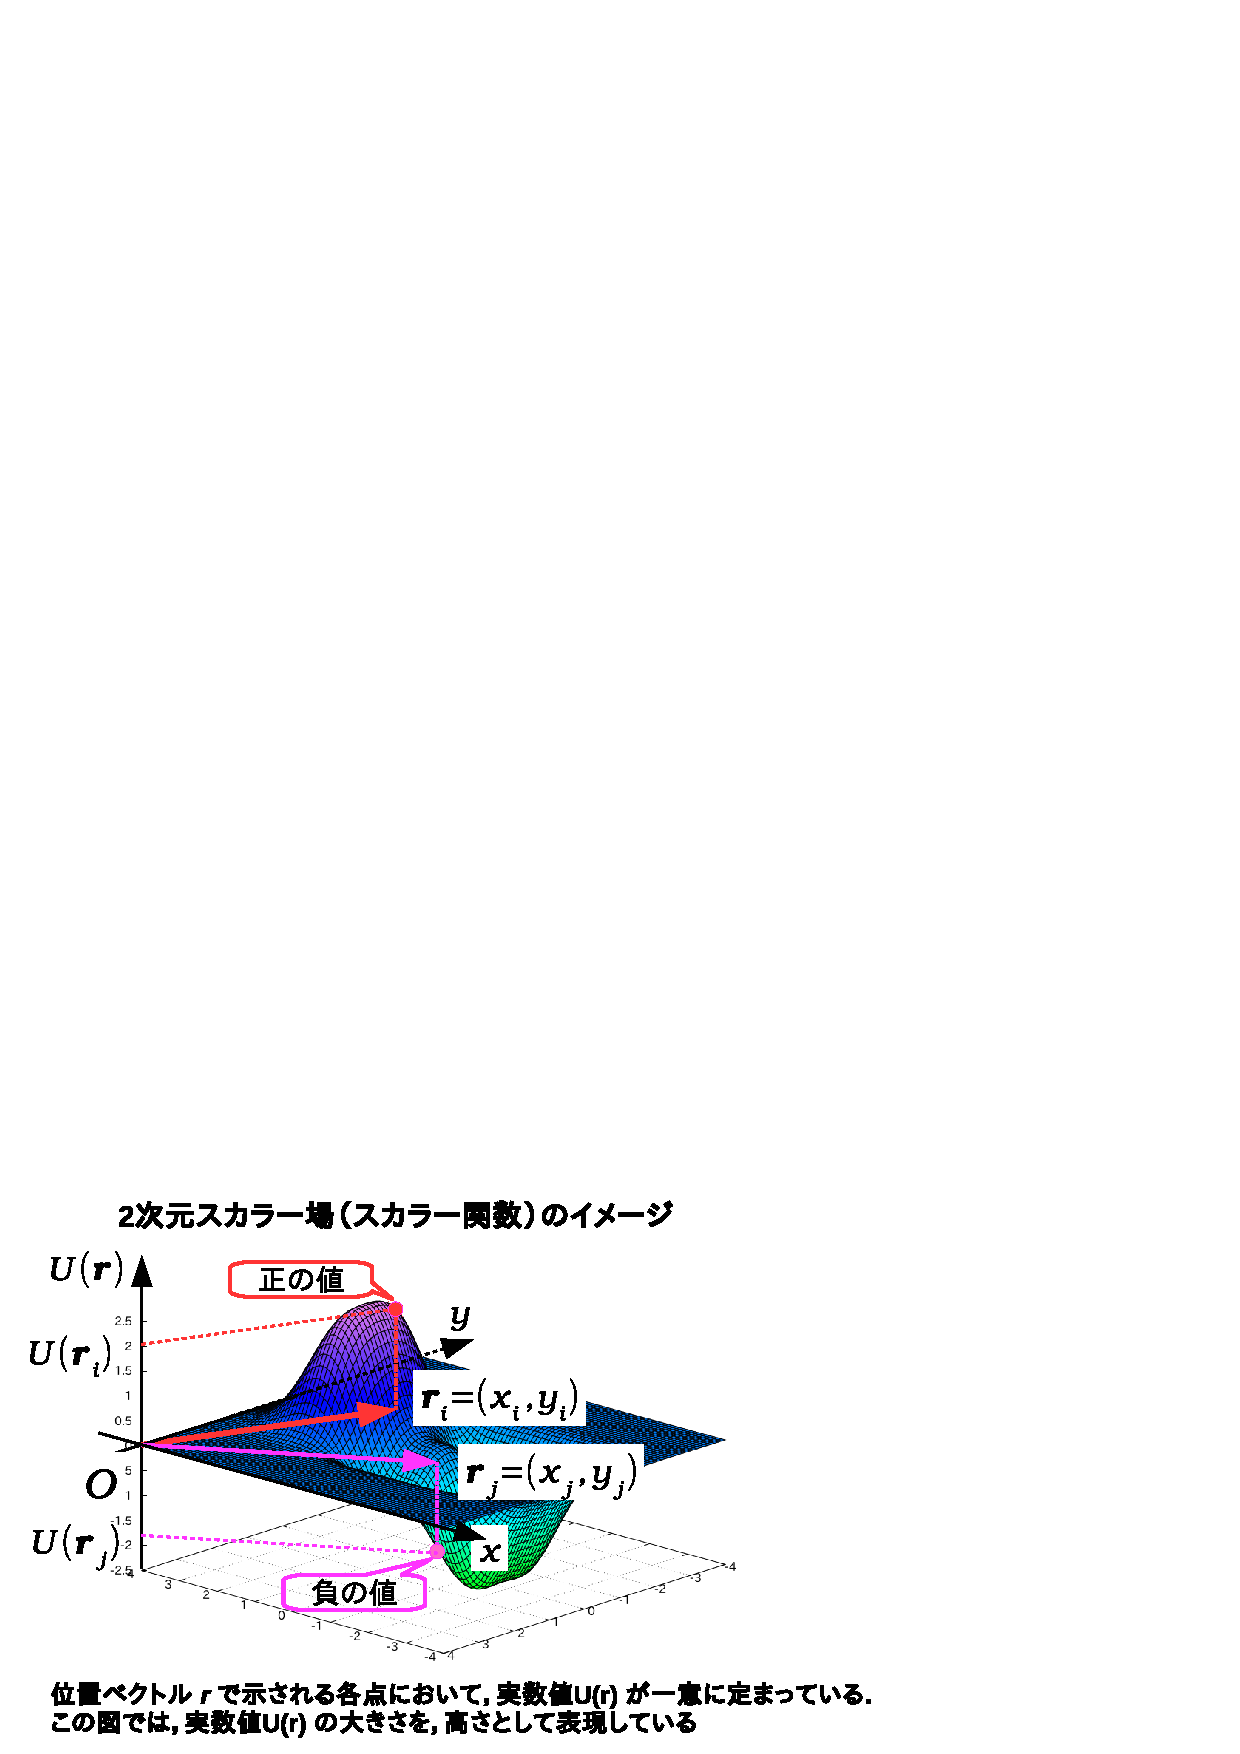
\includegraphics[keepaspectratio, width=7.2cm,height=6.64cm,clip]{scara_function_image001.pdf}
                            \caption{二次元のスカラー関数のイメージ}
                            \label{fig:scara_function_image001}
                        \end{center}
                    \end{figure}


                ポテンシャル$\cdot$エネルギーには地表付近の重力による
                位置エネルギー $mgh$ のほかに,もっと一般的な
                万有引力による位置エネルギーとか,
                電気的なポテンシャル$\cdot$エネルギーがある.
                ポテンシャル$\cdot$エネルギーといった時はこれらを総称していう時もあり,
                注意が必要である.
            \end{mysmallsec}

            \begin{mysmallsec}{運動エネルギーの定義}
                運動エネルギー $T$ についても,改めて定義する.
                    \begin{myshadebox}{運動エネルギーの定義}
                        運動エネルギー $T$ を,次式で定義する.
                        \begin{align}
                        T := \frac{1}{2}mv^{2}
                        \end{align}
                    \end{myshadebox}

                なぜ運動エネルギーというかについては,
                この式がエネルギーの単位をもち,かつ,速度だけによって
                その値が決まるからと考えればよいと思う.
            \end{mysmallsec}

            \begin{mysmallsec}{エネルギー関数 $E$ の独立変数}
                運動エネルギーは速度の関数として捉えられる
                    \footnote{
                        上で運動量表示もできることを示したが,ここでは速度表示の運動エネルギーを
                        考える.
                    }.
                これを,$T=T(\dot{\br})$ と表す.
                また同様に,ポテンシャル$\cdot$エネルギーは位置座標の関数として捉えることができ,
                これを $U=U(\br)$ と書く.
                従って,力学エネルギーは速度と位置の関数である考えられる.なぜなら,
                \begin{align}
                E(\dot{\br},\,\br)=T(\dot{\br})+U(\br)
                \end{align}
                と書けるからである.
            \end{mysmallsec}

            \begin{mysmallsec}{エネルギー保存則}
                さて,力学的エネルギー保存の法則を式(\ref{b})のように書いても
                よいが,「保存則」というからには,時間に依存していないということを
                式で表現しておきたい.そこで,上式の力学的エネルギー $E$ を時間微分して,
                その結果が 0 であるというように表現する形に書き換えておく.
                            \begin{myshadebox}{力学的エネルギー保存の法則}
                                力学的エネルギー保存の法則は,次式によって表される.
                                \begin{align}
                                    \frac{\df E}{\df t}=0
                                \end{align}
                            \end{myshadebox}

                このように考えられる理由は,物体の運動エネルギーとポテンシャル$\cdot$エネルギーの和 $E$ が
                時間変化しないという前提があるからである.
                物体の運動エネルギーと位置エネルギーが時間変化するとき,
                すなわち,$T=T(\dot{\br},\,t)$,$U=U(\br,\,t)$ であるとき
                は,一般には保存則は成り立たない.物体のエネルギーが時間変化するということは,物体は外か
                ら仕事を受けてエネルギーをもらう(とられる)からである.仕事とは外力が引き起こすものであり,
                つまり,「物体に外力が働くときには,力学的エネルギー保存の法則は成り立たない」とい
                える.式で書けば以下の通り.

                この場合の力学的エネルギーは時間 $t$ を変数に含み,
                \begin{align}
                E(\dot{\br},\,\br,\,t)
                =T(\dot{\br},\,t)+U(\br,\,t)
                \end{align}
                と書かれる.時間 $t$ で微分すると,
                \begin{align*}
                \frac{\rd E(\dot{\br},\,\br,\,t)}{\rd t}
                &=\frac{\rd }{\rd t}\biggl\{ T(\dot{\br},\,t)+ U(\br,\,t)\biggr\} \\
                &=\frac{\rd T(\dot{\br},\,t)}{\rd t}+\frac{\rd U(\br,\,t)}{\rd t}
                \end{align*}
                この式の最右辺は0ではなく,時間 $t$ を変数に含む関数である.これを
                簡単に $\alpha (\dot{\br},\,\br,\,t)$ と
                書くことにしよう.すると式は,
                \begin{align}
                \therefore \quad
                \frac{\rd E(\dot{\br},\,\br,\,t)}{\rd t}
                =\alpha (\dot{\br},\,\br,\,t)
                \end{align}
                というように,エネルギー保存則の時間微分は,時間に依存することがはっきりとわかる.

                この関数 $\alpha (\dot{\br},\,\br,\,t)$ の具体的な形は,
                運動エネルギーとポテンシャル$\cdot$エネルギーが
                どのように時間に依存しているかによる.
                この関数 $\alpha(\dot{\br},\,\br,\,t)$ が
                物体のエネルギーの変化量である.

                従って \textbf{外力が物体に働くとき,力学的エネルギーは
                保存しない} ということになる.しかし,もっと広く考えて,外力を含んだ系を
                考えるならば,エネルギーは保存している.これを \textbf{エネルギー保存の法則} という.
                この法則は経験的事実によって,与えられる法則であり,この法則が破られた現象は
                ないとされる.
                (この場合,力学的エネルギーが保存するわけではない.
                外力によって生じた熱力学的エネルギーや電磁気的エネルギーのことをいう.)
            \end{mysmallsec}

            \begin{mysmallsec}{まとめ}
                説明が長くなってしまったが,以上によって,ニュートンの運動方程式から,
                力学的エネルギー保存の法則を導いたことになる.整理しよう.
                まず,ニュートンの運動方程式を認めた($m\textit{\textbf{a}}=\bF$).これは
                力学の出発点となる方程式である.その次に,
                仕事という概念を導入し($W=\bF\cdot \Delta \textit{\textbf{s}}$),
                そこから力学的エネルギーという概念を,運動エネルギーと位置エネルギーの
                2種類のエネルギーの和であると定義した($E=T+U$).そして,
                力学的エネルギーは時間によらず一定値を保つことを
                発見した.

                従って,ニュートンの運動方程式から,
                力学的エネルギー保存の法則を見出したことになる.
            \end{mysmallsec}

            \begin{memo}{注意}
                但し,この $\bF$ は \textbf{保存力} であるとして
                いることを忘れてはならない.
                保存力については後の\ref{PF}で確認することだが,
                ここでは,「力のする仕事が経路によらず,始端と終点
                によってだけ決定されるならば,この力は保存力である」
                と考えてもらいたい.
            \end{memo}


%       %======================================================================
%       %  SubSection
%       %======================================================================
        \subsection{万有引力によるポテンシャル$\cdot$エネルギー}
            ポテンシャル$\cdot$エネルギーの定義を得たので,それを具体的に計算してみる.その例として,
            万有引力によるポテンシャル$\cdot$エネルギーを考える.
            ただ単に,ポテンシャル$\cdot$エネルギーの定義
            式(\ref{eq:PE})に,万有引力を代入すればよいだけである.では,
            早速計算する.

            万有引力は,式(\ref{Grav})によって
                \begin{align}
                    \bF_{\rm{AB}}
                    = -G\frac{m_{\rm{A}}m_{\rm{B}}}{{\left| \br_{A}
                    -\br_{B} \right|}^{2}}
                    \frac{\br_{A}-\br_{B}}{\left| \br_{A}
                    -\br_{B} \right|}
                \end{align}
            と書かれた.ここでは, 質量 $m_{\rm{A}}$ によるポテンシャル$\cdot$エネルギーを考える.
            式変形が煩雑にならないように,
                \begin{align*}
                \br:=\br_{A}-\br_{B}
                \end{align*}
            とおく.
                \begin{align}
                    \bF_{\rm{AB}}
                    = -G\frac{m_{\rm{A}}m_{\rm{B}}}{{\left| \br \right|}^{2}}
                    \frac{\br}{\left| \br \right|}
                \end{align}
            これを,ポテンシャル$\cdot$エネルギーの定義式(\ref{eq:PE})に代入すると,
                \begin{align}
                    U&=-\int \bF_{\rm{AB}}\cdot \df\br  \notag \\
                     &=\int G\frac{m_{\rm{A}}m_{\rm{B}}}{{\left| \br \right|}^{2}}
                    \frac{\br}{\left| \br \right|} \cdot \df\br \notag \\
                     &=Gm_{\rm{A}}m_{\rm{B}}\int \frac{1}{\left| \br \right|^{2}}\df\br \notag \\
                     \therefore \quad U
                     &=-Gm_{\rm{A}}m_{\rm{B}}\frac{1}{\left| \br \right|}
                \end{align}
            と計算される.
            $\br:=\br_{A}-\br_{B}$ を思い出せば,次のようになる.
                \begin{myshadebox}{重力ポテンシャル}
                    重力ポテンシャルは次式で定義される.
                    \begin{align}\label{eq:Grav_1}
                        U=-G\frac{m_{\rm{A}}m_{\rm{B}}}{\left| \br_{A}-\br_{B}\right|}
                    \end{align}
                \end{myshadebox}

            この式(\ref{eq:Grav_1})が質量 $m_{\mathrm{A}}$ が
            その周りに生じさせるポテンシャル$\cdot$エネルギーである.
            このようなポテンシャルを \textbf{重力ポテンシャル} いう.

%       %======================================================================
%       %  SubSection
%       %======================================================================
        \subsection{保存力}\label{PF}
                    今までは,力の存在を仮定して,エネルギーを考えていた.しかし,あくまで仮定しているだけであって,
                    決してはっきりとした概念ではない.ならば逆に,エネルギーを仮定して
                    力を導くことを考えてもよいだろう.
                    力とエネルギーのどちらを基礎とするかは,
                    理論がスマートになる方をとるべきだ.
                    エネルギーを仮定して,力を導出する方が現代的な考え方である.
                    ポテンシャル$\cdot$エネルギーの定義式を力 $\bF$ について
                    解く.$\bF=\left( F_{x}, F_{y},F_{z}\right)$ とする.
                    また,$\df\br=\left( \df x ,\df y ,\df z \right)$ とする.
                        \begin{align}
                            U &= -\int \bF\cdot \df\br \notag \\
                              &= -\int \left( F_{x}\df x+F_{y}\df y+F_{z}\df z \right)
                        \end{align}
                    ここで,$\rd U/\rd x$ を計算すると,
                        \begin{align}
                            \frac{\rd U}{\rd x}=-F_{x}
                        \end{align}
                    となる.ここで記号 $\rd U/\rd x$ の $\rd/\rd x$ は,
                    ($U$ を)“$x$ について微分する”ということである.その際,その他の変数($y$,$z$)は
                    定数とみなすと約束する.$x$ 方向の関数の変化度を知りたいときに,
                    用いる概念である.このような微分の仕方を \textbf{偏微分} という.

                    $y$,$z$ 方向についても同様に考えて,
                        \begin{align}
                        \frac{\rd U}{\rd y}&=-F_{y} \\
                        \notag \\
                        \frac{\rd U}{\rd z}&=-F_{z}
                        \end{align}
                    以上より,
                        \begin{align}\label{hozonryoku}
                            \left( \frac{\rd U}{\rd x} , \frac{\rd U}{\rd y},
                            \frac{\rd U}{\rd z}\right)
                            &=\left( -F_{x} , -F_{y} ,-F_{z} \right) \notag \\
                            \therefore \quad \bF
                            &=-\left( \frac{\rd U}{\rd x} ,
                            \frac{\rd U}{\rd y},
                            \frac{\rd U}{\rd z}\right)
                        \end{align}
                    を得る.ここで,次の微分演算子を定義する.
                        \begin{align}
                        \dgrad:= \left( \frac{\rd}{\rd x} , \frac{\rd}{\rd y},
                        \frac{\rd}{\rd z}\right)
                        \end{align}
                    (この記号の図形的なイメージは次項目で説明する.ここでは
                    とりあえず,記号として受けいれてほしい.)

                    この微分演算子は,$U$ の $x$,$y$,$z$ の3方向の傾きを求める演算子である.つまり,
                    空間の \textbf{勾配}
                        \footnote{
                            「勾配」とは,
                            面の傾斜の度合いのことをいう.例えば,道路の坂
                            が急であるとき,「この坂は急勾配である」といった使い方がされる.
                        }
                    を求める演算子と言える.$\dgrad$ を「グラディエント」と読む.
                    式(\ref{hozonryoku})を
                        \begin{align}
                            \bF=-\left( \frac{\rd}{\rd x} ,
                            \frac{\rd}{\rd y},
                            \frac{\rd}{\rd z}\right)U
                        \end{align} と変形する.そして,$\dgrad$ を
                    用いて,\\
                            \begin{align}
                                \bF=-\mathrm{grad\,} U
                            \end{align}
                    と書ける.
                    この式より,ポテンシャル$\cdot$エネルギーを仮定して力を導出するという意味として捉え直せる.

                    なので,ここで思い切って,保存力が生じている理由は,その周囲にポテンシャルエネルギーがあるからである,
                    と考えなおそう.保存力がポテンシャルエネルギーを周囲に作るというイメージよりも,そもそも最初は
                    ポテンシャルエネルギーがそこにあり,我々は,ポテンシャルエネルギーそのものを見ることはできないが,
                    その一端を保存力として観測していると考える方が,自然である.力を仮定してポテンシャルエネルギーを
                    導く場合には,試験用の質点を用意して至るところに置き,ポテンシャルエネルギーの分布を得るとになる
                        \footnote{
                                保存力を線積分するイメージ.
                        }.
                    しかし,ポテンシャルエネルギーを仮定すれば,ポテンシャルエネルギーの勾配($\dgrad$)を取るだけで,
                    保存力がえられるのだ.

                    こう考えなおすと,保存力 $\bF$ は,以下のように,ポテンシャルエネルギー $U(\br)$ の勾配で与えられる.
                        \begin{align*}
                                \bF = -\dgrad U(\br) = -\frac{\rd U(\br)}{\rd \br}.
                        \end{align*}
                                        両辺を始点 ${\br}_{\mbox{a}}$ から終点 ${\br}_{\mbox{b}}$ で積分すると,
                        \begin{align}\label{eq:forceF_and_potentialU}
                                   \int_{\br_{\mbox{a}}} ^{\br_{\mbox{b}}}\bF \cdot \br
                                   &=    \int_{\br_{\mbox{a}}} ^{\br_{\mbox{b}}}
                                           \left(
                                                -\frac{\rd U(\br)}{\rd \br}
                                           \right) \notag \\
                                   &=  - \int_{\br_{\mbox{a}}} ^{\br_{\mbox{b}}} \df U(\br) \notag \\
                                   &=  - \left( U(\br_{\mbox{b}}) - U(\br_{\mbox{a}}) \right) \notag \\
                                   &=  - U(\br_{\mbox{b}}) - ( - U(\br_{\mbox{a}}) ) \notag \\
                                   &=  \mbox{(一定)}
                        \end{align}
                    最初の位置 $\br_{\mbox{a}}$ でのポテンシャルエネルギー $-U(\br_{\mbox{a}})$ と移動後の位置 $\br_{\mbox{b}}$ の
                    ポテンシャルエネルギー $-U(\br_{\mbox{b}})$ の差のみで表せるという結果を得た.つまり,経路に依存していない.
                    どのような経路をとっても,始点と終点を指定するだけで,線積分が計算できるのだ,この線積分は位置と力の内積に
                    関するものであり,すなわち,始点から終点までになした仕事にほかならない,とどのつまり,の式は,
                    物体を $\br_{\mbox{a}}$ から $\br_{\mbox{b}}$ まで移動させるのに必要なエネルギーを表しているということだ.

                                        ただこのままでは,位置 $\br$ のポテンシャルエネルギーを $-U(\br)$ と書いた場合,終点は $-U(\br)$ だが始点が
                                        定まっていないため,値が定まらない.そこで,基準点を設けて,それに対するポテンシャルエネルギーを定義しよう.

                                        一般に,$A-B$ という式を見た場合,$A$ は $B$ を基準とした値であると解釈できる.例えば,$A=5$,$B=3$ とした時,
                                        $A-B=2$ であり,$A$ は絶対値5だけど $B$ から見ればその差は2である.
                                                \footnote{
                                                        このような見方を,$B$を基準にしてみると表現する
                                                }.
                                    同様に,$- U(\br_{\mbox{b}}) - ( - U(\br_{\mbox{a}}) )$ は $- U(\br_{\mbox{a}})$ を基準にしたときの,
                                    $- U(\br_{\mbox{b}})$ の値と解釈できる.そこで,$- U(\br_{\mbox{a}})=0$ となるような点
                                        \footnote{
                                                このような点が現実にあるわけでない.人間が勝手に基準となる点を設定しなければいけない.$- U(\br_{\mbox{a}})=0$ と
                                                できる点を適宜用意する必要がある.多くの場合は,無限遠点を基準点に取ることが多い.無限遠点とは,これまた曖昧な
                                                概念だが,ここから遠ざかって見えなくなった先の更に先というイメージで十分だ.
                                                実際,無限遠点はここだと示すことはできず,想像するより他にない.問題によっては基準点を別の点にとったほうが
                                                計算しやすい場合がある.その場合は,基準点を最も計算しやすい適切な点に再設定すれば良い.どうせ基準点は計算結果に
                                                影響しないのだから(基準点を決めないと不定積分になり不定性が残るが,基準点があれば定積分となり不定性はなくなる).
                                        }
                                    を基準点にとると,定義する.
                                    こうすることで,始点を暗黙裏に仮定することにより,毎回基準点を示すことなく,ポテンシャルエネルギーを考えることができる.
                                    ただ,基準点を示さないのが当たり前になってくると,ポテンシャルエネルギーがそもそも基準点をとるということを忘れがちであるので,
                                    この点は注意が必要だ
                                        \footnote{
                                                簡略化した記述は効率的だが,記述しないがゆえに見えなくなってしまうというジレンマがある.
                                                慣れれば(当たり前になれば)当然のこととして捉えられるが,なかなか難しい.
                                        }.
                                    このように,より簡略化した記述では,ポテンシャルエネルギーと保存力の関係式は以下のようになる
                                        \footnote{
                                                まず,式(\ref{eq:forceF_and_potentialU})で,始点は $-U(\br_{\mbox{a}})=0$ となる基準点を選ぶのであった.
                                                また,終点 $-U(\br_{\mbox{b}})$ の添字 $\mbox{b}$ も明示しなくても,常に終点を示すものであると読み取ることが可能なので,
                                                記述省略してしまおう.
                                        }.
                        \begin{align*}
                                   \int \bF \cdot \br  =  - U(\br)
                        \end{align*}

                    一般には,全ての力がポテンシャル$\cdot$エネルギーから導出されるわけではない.つまり,非保存力であるものもある.
                    この場合には,非保存力 $\bar{\bF}$ のする仕事を $W$ として,
                        \begin{align}
                            \bar{\bF}
                            = -\frac{\rd W}{\rd\br}
                        \end{align}
                    と書ける.もちろん,保存力と非保存力の両方を含む場合は,力の重ね合わせの原理から,
                        \begin{align}
                            \bF+\bar{\bF}
                            = -\frac{\rd U}{\rd\br}
                              -\frac{\rd W}{\rd\br}
                        \end{align}
                    である.
                    \begin{figure}[hbt]
                        \begin{center}
                            \includegraphicslarge{hozonryoku.pdf}
                            \caption{重力から受ける仕事は鉛直方向のみ}
                            \label{fig:hozonryoku}
                        \end{center}
                    \end{figure}

%       %======================================================================
%       %  SubSection
%       %======================================================================
        \subsection{勾配}
                    演算子 $\dgrad$ は,以下のように定義される量であることを,
                    前項目で確認した.
                        \begin{align}
                        \dgrad:= \left( \frac{\rd}{\rd x} , \frac{\rd}{\rd y},
                        \frac{\rd}{\rd z}\right)
                        \end{align}
                    この定義式をイメージすることが,この項目の目標である.

                    唐突ではあるが,
                    まず,連続でなめらかな1変数関数 $f_{1}=f(x)$ のグラフの接線の傾き $f'_{1}$ 考える.
                    $f'_{1}$ は $f_{1}$ の $x$ に関する微分であり,
                    \begin{align}
                    f'_{1}=\frac{\df }{\df x}f_{1}
                    \end{align}
                    のように与えられる.(図\ref{fig:grad1}参照)
                    これが1変数関数の場合である.

                \begin{figure}[hbt]
                    \begin{tabular}{cc}
                        \begin{minipage}{0.5\hsize}
                                    \begin{center}
                                        \includegraphicsdouble{grad1.pdf}

                                        (A) 1変数関数
                                        \label{fig:grad1}
                                    \end{center}
                        \end{minipage}
                        \begin{minipage}{0.5\hsize}
                                    \begin{center}
                                        \includegraphicsdouble{grad2.pdf}

                                        (B) 2変数関数
                                        \label{fig:grad2}
                                    \end{center}
                        \end{minipage}
                    \end{tabular}

                        \caption{傾き}
                \end{figure}

                    この考えを,
                    2変数関数 $f_{2}=f_{2}(x,\,y)$ の場合について拡張してみる.
                    関数 $f_{2}=f_{2}(x,\,y)$ は図\ref{fig:grad2}のように
                    描くことができる.もちろん,関数 $f_{2}=f_{2}(x,\,y)$ は連続で
                    なめらかであることを仮定している.関数 $f_{2}=f_{2}(x,\,y)$ を,
                    点$(x,\,y)$ を代入したときの高さを表していると考えれば,
                    このような点を全て集めると,
                    それは\textbf{曲面}をなしていると言える
                        \footnote{
                            つまり,$f(x,\,y)$ は幾何学的には,曲面を表す関数としてイメージされる.
                        }.
                    1変数関数における曲線が,
                    2変数関数になると,曲面になるのである.
                    従って,2変数の場合には,
                    直線の接線の傾きを考えるのでは不十分であり,
                    面の \textbf{勾配} を考えなければいけない
                        \footnote{
                                「勾配」とは面の傾き具合を表す語彙.1次元の場合は「傾き」という
                                表現を使ったが,2次元の場合は「勾配」と言い表す.2次元以上の場合
                                でも「勾配」という.
                        }.
                    そこで,図\ref{fig:grad2}の青い線で描いたような,
                    接面の勾配を考えるのである.この接面の勾配を考える.
                    図\ref{fig:grad2}では説明しにくいので,改めて,
                    図\ref{fig:grad3}に必要な部分だけ書き改めることにする.
                    (若干異なっているが許してほしい.)

                \begin{figure}[hbt]
                    \begin{tabular}{cc}
                        \begin{minipage}{0.5\hsize}
                                    \begin{center}
                                        \includegraphicsdouble{grad3.pdf}

                                        (A) 2変数関数の傾き
                                        \label{fig:grad3}
                                    \end{center}
                        \end{minipage}
                        \begin{minipage}{0.5\hsize}
                                    \begin{center}
                                        \includegraphicsdouble{grad4.pdf}

                                        (B) 接面の勾配
                                        \label{fig:grad4}
                                    \end{center}
                        \end{minipage}
                    \end{tabular}

                        \caption{面の傾き}
                \end{figure}

                図の緑の太線で示した曲面部分に接する平面を
                考える.図の $A$ は $x$--$y$ 平面上の点を表している.そのような平面のことを \textbf{接面} と
                いうことにする.この接面の勾配を
                示すには,$x$ 方向の接面の傾きと,$y$ 方向の
                接面の傾きを考えればよい.従って,それぞれの方向に \textbf{偏微分} すればよい.
                前項目では偏微分の定義には触れなかったので,
                ここでは簡単に偏微分の定義式を示しておこうと思う.

%       %======================================================================
%       %  SubSection
%       %======================================================================
        \subsection{保存力と $\dgrad$ の図的イメージ}
                偏微分は,グニャグニャ曲がっている面のある一点における
                傾きを計算する場合に役に立つ.面の傾きを考えるには,
                2つの方向の傾きを考える必要がある.しかし,2方向の傾き
                を同時に考えることは難しい.そのため,一方向ずつ傾きを
                計算する.一方向の傾きを計算するには,曲線の傾きと
                同じように考えられる.そのとき,残りのもう1方向は定数として
                扱う.

                例えば,接面の $x$ 方向の傾きを考える場合,$y$ 座標を一時的に固定して定数と
                して扱い,$x$ 方向のみに着目し微分する.偏微分の記号は通常の微分と区別するために,
                $\rd$ という文字が使われる.具体的には,以下の通り.
                \begin{align}
                    \frac{\rd }{\rd x}f(x,\,y) := \lim_{\Delta x \to 0} \frac{f(x+\Delta x,\, y) - f(x,\,y)}{\Delta x}.
                \end{align}

                接面の $x$ 方向の傾きも同様に考えて,
                \begin{align}
                    \frac{\rd }{\rd y}f(x,\,y) := \lim_{\Delta y \to 0} \frac{f(x,\,y+\Delta y) - f(x,\,y)}{\Delta y}.
                \end{align}

                これらを用いて,曲面f上の点($x,\,y$)の接面は
                    \begin{equation*}
                        \left( \frac{\rd }{\rd x}f(x,\,y) \,,\; \frac{\rd }{\rd y}f(x,\,y) \right)
                    \end{equation*}
                と表現できる.ただ,$f$ の独立変数をいちいち書いていると煩雑なので,省略する場合が多い
                    \footnote{
                        偏微分の対象となる方向は分母でわかるし,他の変数は定数扱いなので無理して明示する必要もない.
                        問題になるとしたら,独立変数の個数がわからなくなってしまうことだが,前もって明記しておけば
                        覚えていられるだろう.
                    }.
                    \begin{equation*}
                        \left( \frac{\rd }{\rd x}f \,,\; \frac{\rd }{\rd y}f \right)
                    \end{equation*}
                もっと省略して,以下のように書かれることもある($f$ をカッコの外に出した).
                    \begin{equation*}
                        \left( \frac{\rd }{\rd x} \,,\;  \frac{\rd }{\rd y} \right) f
                    \end{equation*}
                こうすると,式に意味を与えやすい
                    \footnote{
                        ただし,注意したいのは,
                        $\displaystyle \left( \frac{\rd }{\rd x} \,,\; \frac{\rd }{\rd y} \right)$ と $f$ の積
                        と解釈してはいけない,ということである.
                    }.
                こうすると,表現上,$f$ に対して
                操作 $\displaystyle \left( \frac{\rd }{\rd x} \,,\; \frac{\rd }{\rd y} \right)$ を施すことで,
                接面が現れると読むことができる.物理学では,
                    \begin{equation*}
                        \dgrad := \left( \frac{\rd }{\rd x} \,,\; \frac{\rd }{\rd y} \right)
                    \end{equation*}
                として,単に
                    \begin{equation*}
                        \dgrad f
                    \end{equation*}
                と書かれる.ポテンシャルエネルギーを考える場合には,$f=-U(\br)$ とすればいい.

                    ポテンシャルエネルギーの関数 $U(\br)$ が与えられている時,保存力 $\bF(\br)$ は以下のように計算できる.
                    \begin{align*}
                        \bF (\br) &= - \dgrad U(\br) \\
                                  &= -\left(
                                                \frac{\rd}{\rd x}\,,\;
                                                \frac{\rd}{\rd y}\,,\;
                                                \frac{\rd}{\rd z}
                                     \right)  U(\br) \\
                                  &=  \left(
                                        - \frac{\rd U(\br)}{\rd x}\,,\;
                                        - \frac{\rd U(\br)}{\rd y}\,,\;
                                        - \frac{\rd U(\br)}{\rd z}
                                     \right)
                        \end{align*}

                上式で表されるポテンシャルエネルギーと保存力のイメージを,以下に表現しておこう.
                    \begin{figure}[hbt]
                        \begin{center}
                            \includegraphicslarge{scara_function_image002.pdf}
                            \caption{ポテンシャルエネルギーと保存力}
                            \label{fig:sensekibun_shukaisekibun_002}
                        \end{center}
                    \end{figure}

                この図で注意してみて欲しいのは,ポテンシャルエネルギーを2次元で表していることである.
                実際の空間はは3次元だが,これだと図に表すことができない
                        \footnote{
                            関数の取る値をグラフで示すための次元が1つ必要になるからである.
                            ここでは,本来の3次元の内から1次元減らし,代わりに関数のとる
                            値を山として表現している.
                        }.

%       %======================================================================
%       %  Memo
%       %======================================================================
        \begin{memo}{$\rd / \rd \br$ という表現について}
            上で使ってしまったが,便利でよく使われてしまう表現に,
                        \begin{equation*}
                                \frac{\rd f(\br)}{\rd \br}
                        \end{equation*}
            というものがある.

            ベクトル $\br$ で割り算しているように見えるが,そうではない
                \footnote{
                    "ベクトル除算" なんてものはない.
                }.
            本当は,
                        \begin{align*}
                                \frac{\rd f(\br)}{\rd \br}
                                &=
                                    \left(
                                      \frac{\rd f(\br)}{\rd x} \,,\;
                                      \frac{\rd f(\br)}{\rd y} \,,\;
                                      \frac{\rd f(\br)}{\rd z}
                                \right) \\
                                &=
                                    \left(
                                      \frac{\rd f(x,\,y,\,z)}{\rd x} \,,\;
                                      \frac{\rd f(x,\,y,\,z)}{\rd y} \,,\;
                                      \frac{\rd f(x,\,y,\,z)}{\rd z}
                                \right)
                                \end{align*}
                    という意味で使われるものである.紛らわしいが,よく見かける表現なので注意しておきたい.
                    こういう表現は,疑問や誤解を招くので,避けたほうが良い
                        \footnote{
                            勾配演算子 $\dgrad$ や後で紹介する数学記号 $\nabla$ を使って表現すべき.
                        }.
        \end{memo}

%       %======================================================================
%       %  SubSection
%       %======================================================================
        \subsection{保存力と周回積分}\label{subsec:hozonryoku_to_shukaisekibun}
                        ポテンシャルエネルギー $U(\br)$ のみの場合などのように,外力が働かない時,
                        始点Aと終点Bの2つの位置ベクトルを定めると,AからBまでの経路Cは無数に存在するが,
                        AからBまで物体を移動させる仕事はその経路に依存せず,一定値をとる.
                        \begin{equation*}
                                \oint_{\mbox{C}} \bF (\br) \cdot \df \br = U(\br_{\mbox{b}}) - U(\br_{\mbox{a}}).
                        \end{equation*}
                        このような性質を持つ関数で表される力のことを,\textbf{保存力} と言うことはすでに記述した.
            特に注目すべきはことは,B$=$Aとした時(始点と終点を同じ点にした場合),
                        \begin{equation*}
                                \oint_{\mbox{C}} \bF (\br) \cdot \df \br = U(\br_{\mbox{a}}) - U(\br_{\mbox{a}}) = 0
                        \end{equation*}
                        となることである.


                        ポテンシャルエネルギー値 $U(\br)$ がベクトル $\br$ に対して一意に定まる場合,
                        $U$ により生じる力は保存力となる.
                    \begin{figure}[hbt]
                        \begin{center}
                            \includegraphicslarge{sensekibun_shukaisekibun_001.pdf}
                            \caption{保存力の性質}
                            \label{fig:sensekibun_shukaisekibun_001}
                        \end{center}
                    \end{figure}


                        しかし,例えば下図のように,ポテンシャルエネルギー値 $U(\br)$ がベクトル $\br$ に対して
                        一意に\textbf{定まらない}場合,$U$ により生じる力は保存力ではない.
                    \begin{figure}[hbt]
                        \begin{center}
                            \includegraphicslarge{sensekibun_shukaisekibun_004.pdf}
                            \caption{保存力でない場合}
                            \label{fig:sensekibun_shukaisekibun_004}
                        \end{center}
                    \end{figure}

%   %==========================================================================
%   %  Section
%   %==========================================================================
    \section{エネルギーと運動量}
        エネルギーと運動量は似たような概念だ.この2つの間には大切な関係がある.
        特に,量子力学を学習するとこの関係が顕著に現れてくる.
        運動量 $\bp$ をもつ物体に関与する力を保存力とし,$\bF$ とする.
                \footnote{
                        ここでは保存則について考えているのであった.保存力以外の外力が
                        働く場合は,運動量保存則とエネルギー保存則は成立しないの.
                }.
        運動量表示の運動方程式は
                        \begin{align*}
                        \frac{\df \bp}{\df t} = \bF.
                        \end{align*}
        であった.$t$ は時間である.
        ところで,保存力である $\bF$ はポテンシャルエネルギー $U(\br)$ を導入すると,
                        \begin{align*}
                        \bF = -\frac{\rd U}{\rd \br}.
                        \end{align*}
        ここで,$E(\br)=-U(\br)$ と置いてしまおう.
                        \begin{align*}
                        \bF = \frac{\rd E}{\rd \br}.
                        \end{align*}
                要するに,$\rd U/\rd \br$ と $\rd E/\rd \br$ は共に力の次元を持っている,
                $\bF$ を消去して,それぞれの次元を考えると,
                        \begin{align*}
                        \left[\frac{\df \bp}{\df t}\right] = \left[\frac{\rd E}{\rd \br}\right]
                        \end{align*}
                微分記号と偏微分記号は不要.
                        \begin{align*}
                        \frac{[\bp]}{[t]} = \frac{[E]}{[\br]}
                        \end{align*}
                これを以下のように書きなおす.
                        \begin{align}
                                [\bp] \cdot [\br] = [E][t].
                        \end{align}
            もしかしたら,$\br=(x,\,0,\,0)$,$\bp=({p}_{x},\,0,\,0)$ としたほうがわかりやすいかもしれない.
                        \begin{align*}
                                {p}_{x}x = Et.
                        \end{align*}



\chapter{座標変換}
%   %-----------------------------------------------------------------------------------------------
%   %  Input
%   %    File Name : PhysNote_CM_Zahyou.tex
%   %    説明      : 座標について記述する
%   %-----------------------------------------------------------------------------------------------
        \section{座標のとりかた}
\subsection{座標とは}
    空間内の点の位置を指定する手段として,\textbf{座標} はとても重要であり,
    座標なくしては位置を数学的に表すことはできない
        \footnote{
            これ以上に簡潔なものはない,という意味で.
        }.
    今まで主に使ってきた座標は,縦・横・高さの3つの数字であらわされる,\textbf{3次元直交座標} を使っていた.
    しかし,点の位置を指定するのに,この座標系しか考えられないということはない.
    \textbf{3次元空間内の点を表すには,適当に決めた“3つの互いに独立な変数”を用いればよい}.
    座標の取り方は3次元直交座標以外にも,例えば,\textbf{極座標} とか,\textbf{斜交座標} が
    よく取り上げられる.座標によって位置の示し方は異なるが,異なるのは示し方だけであって,どの座標を採用しても
    示される位置に違いはない.極座標を使おうが斜交座標を使おうが,それらを使ってあらわされる位置の特性に
    違いが出るわけではない.

    下手な例えかもしれないが,座標の違いは言葉の違いに似ている.
    現象を英語で表現しようが,日本語で表現しようが,その表現される現象が
    変わるわけではない.ただ,同じ現象を日本語で説明された時と,
    英語で説明された時のイメージ(ニュアンス)は異なるように,
    採用する座標によって主張する部分が変わってくる.極座標は角運動(回転運動)
    を表現するのに簡潔であることが多く,惑星の運動やコマの回転運動などを扱うときは,
    極座標がよく用いられる.

    以下では,座標の種類をいくつか見た後,それらの相互の関係について,考える.
    座標の相互関係は \textbf{座標変換} とう考え方を使って表現される.
    座標変換によって,ある座標から別の座標へ切り替えることが可能になる.
    特に,相対性理論は,座標変換による計算地獄だ.
    ここでは,将来学習する相対性理論も視野に入れつつ,
    座標そのものに対するイメージを習得していこう.

\subsection{直交座標}
    \textbf{直交座標} については説明するまでもない.
    今まで考えてきた $x$,$y$,$z$ を直線軸とし,これらの軸が
    互いに直交するようにとった座標ののことである.
        \begin{figure}[hbt]
            \begin{center}
                \includegraphicsdefault{chokkou.pdf}
                \caption{直交座標}
                \label{fig:chokkou}
            \end{center}
        \end{figure}

\subsection{斜交座標}
    直交座標は各直線軸同士の交わりが,互いに直交していた.
    しかし,直交していない ----- つまり,斜めに交わっていても ,座標として成立する.
    直交していない直線軸で表される座標は \textbf{斜交座標} とよばれる.

    まず,2次元で考えてみよう.直交座標 $x\,$---$\,y$ と,斜交座標 $x'\,$---$\,y'$ の関係
    を考えてみよう.図を描けば図\ref{fig:shakou_chokkou_zahyou}のようになる.
        \begin{figure}[hbt]
            \begin{center}
                \includegraphicsdefault{shakou_chokkou_zahyou.pdf}
                \caption{斜交座標}
                \label{fig:shakou_chokkou_zahyou}
            \end{center}
        \end{figure}

    まず $x'$ を ,$x$ と $y$ で表現することを考えよう.つまり,直交座標 $x\,$---$\,y$ から見た,
    直線 $x'$ の式を考えるのである.直線の式は簡単に書くと,$y=ax+b$ である.$a$ は
    直線の傾きで,$b$ は直線が $y$ 軸と交わる切片である.直線の傾きを知るには,直線の式を
    微分ればよい.
        \begin{equation*}
            \mbox{(直線の傾き)} \; a = \frac{\df y}{\df x}.
        \end{equation*}
    また,今回は,簡単のために
        \footnote{
            「簡単のために」とは,説明が複雑にならないように,条件を簡単にして考えたいということである.
            一般的に考えてしまうと,それ説明するときに式が複雑になり,要点がつかみにくくなってしまう.
            簡単化してしまうと,一般的な議論ができない.しかし,要点をつかむことが大事であるので,
            一般的議論を犠牲にするのである.
        },
    $b=0$ としよう.すると,関係式は次のように簡単になってしまう.
        \begin{align}
            x ' \mbox{の式} : y = \frac{\df y}{\df x}x
        \end{align}

\subsection{極座標}
            極座標の場合の座標変数の取り方は,
            自分の位置する場所を座標原点 O としたとき,
            自分からの距離 $r$ と,水平方向のある1方向を基準にしたときの角度 $\phi$,
            そして,鉛直方向の上向きを基準としたときの角度 $\theta$ の3つの変数を用いる.
            図でイメージするならば図\ref{fig:kyoku2}のようである.但し,
            直交座標との対応関係がわかるように,直交座標も点線で描いている.

           図\ref{fig:kyoku2}のように,
            極座標の3つ独立な座標変数は $(r,\,\theta,\,\phi)$ で
            表現される.それらのとり方は,書いた通りである.
            これらの変数には一応名前がついており,$r$ を \textbf{動径},$\theta$ を \textbf{天頂角},
            $\phi$ を \textbf{方位角} という.
                    \begin{figure}[hbt]
                        \begin{center}
                            \includegraphicsdefault{kyoku2.pdf}
                            \caption{極座標}
                            \label{fig:kyoku2}
                        \end{center}
                    \end{figure}
                    \begin{figure}[hbt]
                        \begin{center}
                            \includegraphicsdefault{kyoku_chokkou.pdf}
                            \caption{直交座標との対応}
                            \label{fig:kyoku_chokkou}
                        \end{center}
                    \end{figure}


            直交座標との関係は,図より
                    \begin{align}
                            \begin{cases}\label{kyoku_chokkou}
                                x=r\sin\theta \cos\varphi \\
                                y=r\sin\theta \sin\varphi \\
                                z=r\cos\theta
                            \end{cases}
                    \end{align}
            となることがわかる.



\subsection{円筒座標}
            円筒座標の場合の座標変数の取り方を説明する.
            そのイメージを図\ref{fig:entou}に描いておくので,
            この図を参照しながら読んでほしい.まず,
            自分の位置する場所を座標原点 O とする.
            そして,この座標原点 O を含むような1つの平面を
            選ぶ.この平面の選び方は複数存在するが,
            そのうちの1つを任意に選ぶとする.図\ref{fig:entou}では $x-y$ 平面に相当する
            ものである.さて,示したい点 $\textit{\textbf{P}}$ から,
            先に指定した平面に垂線を引き,
            垂線の足を $H$ とする.ここでまず一つ目の座標 $z$ を,
            点 $\textit{\textbf{P}}$ から $H$ へ引いた線分の長さとする.
             $\rho$ については座標原点 O から,$x-y$ 平面に
            沿って点 $H$ まで引いた線分の長さというようにとる.
            残りの1つの変数,$\phi$ については,極座標の場合と同様なとり方をする.

            従って,円筒座標で点の位置を示したいときは,$(\rho,\,\phi,\,z)$ と
            いう座標を用いることになる.
                \begin{figure}[hbt]
                    \begin{center}
                        \includegraphicsdefault{entou.pdf}
                        \caption{円筒座標}
                        \label{fig:entou}
                    \end{center}
                \end{figure}


            直交座標との関係は,図より
                    \begin{align}
                            \begin{cases}\label{entou_chokkou}
                                x=\rho\cos\phi \\
                                y=\rho\sin\phi \\
                                z=z
                            \end{cases}
                    \end{align}
            となることがわかる.$z$ 座標は同じである.


\section{異なる座標同士の関係}
\subsection{座標による違い}
                1つの同じ物体(質量:$m$)の運動をみて,二人の観測者がその物体の運動方程式を
                正しく記述したとしよう.運動方程式を書くときには,どのような座標をとるかを
                決める必要がある.座標には,直交座標,極座標など,いろいろな
                表し方があるが,そのどれをとってもよい.

                さて,二人のがそれぞれ書いた運動方程式を比べてみるとき,
                使用した座標が違っていたとしよう.運動方程式の記述の仕方は
                ,使用する座標によって変わってしまう.しかし,2つの運動方程式
                が表す物体の軌跡は,正しく記述されているので,全く同じになるはずである.
                しかし,その関係は,一見してわかりにくいものになるだろう.

                例として,一方の運動方程式を直交座標でかかれたものとし,もう一方を
                極座標でかかれているとしよう.簡単のために,2次元で考え,さらに,
                物体に加わる力は保存力(ポテンシャルは $V(x,\,y)$)であるとしよう.
                直交座標で書かれた運動方程式は,
                    \begin{align}
                        \begin{cases}
                            \displaystyle m\frac{\df^{2} x}{\df t^{2}} = -\frac{\rd V(x,\,y)}{\rd x} \\
                            \displaystyle m\frac{\df^{2} y}{\df t^{2}} = -\frac{\rd V(x,\,y)}{\rd y}
                        \end{cases}
                    \end{align}
                である.同じ運動方程式を,極座標で表すと,
                    \begin{align}
                        \begin{cases}
                            \displaystyle m\biggl\{ \frac{\df^{2} r }{\df t^{2}}  - r\left( \frac{\df \theta}{\df t} \right)^{2} \biggr\}
                                    = -\frac{\rd V(r,\,\theta)}{\rd r} \\
                            \displaystyle m\left( r\frac{\df^{2} \theta }{\df t^{2}} + 2\frac{\df r}{\df t}\frac{\df \theta}{\df t} \right)
                                    = -\frac{1}{r}\frac{\rd V(r,\,\theta)}{\rd \theta}
                        \end{cases}
                    \end{align}
                となる.

                運動方程式を直交座標で表そうが,極座標で表そうが,
                結果として得られる軌道は全く変わらない
                    \footnote{
                        確かに,勝手に選択した座標によって運動方程式を記述しても,結果として
                        得られる物体の運動の軌跡は,1つである.これはこれで,大変驚くべき事だと思う.
                        しかし,不満もあるだろう.運動方程式の形が,座標系によって異なるのである.
                        人間が勝手に決めた座標系によって,運動方程式の形が違うのである.
                        実はこの不満は,解析力学を見てみることで,解決をすることである.
                        ここではしばらく我慢して,異なる座標同士の関係について見ていくことにしたい.
                    }.

                座標は人間が勝手に決められるもので,そのとり方はいろいろある.どの座標を選んでも
                運動の法則を満たし,同じ結果を得ることができる.となると,この座標同士の関係はどう
                なっているかが気になってこよう.

                座標のとり方には,色々な方法があることを確認した.
                次に,それぞれの関係をで考えてみよう.

                    \subsection{直交座標 $\rightarrow$ 斜交座標}
                         直交座標と斜交座標の関係を考えよう.これは,座標同士の関係の中で,
                         最も理解しやすいものである.そしてまた,この関係は物理学ではとても重要な
                         関係である.なので,この関係はどうしても理解したい.
                         感覚的に分かるように,できるだけ細かいステップを踏んで,
                         考えていこう.

\section{座標変換}
                今までは具体的な2つの座標同士の関係を見てきた.
                実用的には,これまでの具体的な関係式のほうが,役に立つ
                ことだろう
                    \footnote{
                        実際の現象を解決するに当たっては,式は具体的に
                        書かれているほうが,使いやすい.多くある関係式
                        から,使いやすい式を選択すればよい.
                    }.
                しかし,理論物理学の目指すところは,一般的に通用する式
                を記述することである.この目標を満足させるためには,任
                意の2つの座標間の,変換関係式を記述ればよい.今までのに
                得た,具体的な関係式を参照しながら,一般的に通用する関
                係式を導いてみよう
                    \footnote{
                        発見的方法で,一般の座標変換式を導くことになる.
                        この方法をとると,「どんな2つの座標系間でも必ず
                        成り立つかどうか」を示す必要が出てくる.しかし,
                        このノートではその証明は省略する.明らかに成立
                        することが,わかるだろうから.いや,面倒臭い
                        から.知りたい場合は,座標変換に関する数学の教
                        科書や,物理学の教科書を参照しよう.
                    }.

                \subsection{座標系の表現の仕方}
                    さて,任意の2つの座標系を文字で表さないといけない.
                    この2つの座標系をそれぞれ,$x$ 座標系と $X$ 座標系
                    のように,小文字と大文字で区別することにしよう.そし
                    て,座標変換を考えるには,基準とする座標系を$x$ 座
                    標系と $X$ 座標系のどちらかに設定すると楽である.
                    ここでは,$x$ 座標系を基準の座標系としよう.基準の
                    座標系とは,もちろん,私に対して静止している座標系
                    のことである.

\section{座標変換と運動方程式}

            \begin{mycomment}
            ある慣性系で,物体の運動方程式をたてる.そして,その慣性系とは別の慣性系に移り,同じ物体の運動方程式を立てたとき,
            その運動方程式は形を変えてしまうのだろうか.結論をいうと,形を変えないのである.それを説明していく.慣性系から
            別の慣性系に移ることを,\textbf{ガリレイ変換} という.ここでいう変換とは \textbf{座標変換} のことである.座標変換をする
            ということには,「物体の観測をする立場を変えてみる」といった意味がある.観測する立場というのは,例えば,
            別の速度(等速度)で運動している状況での観測とか,加速度運動している状況での観測とかということである.
            \end{mycomment}

\subsection{ガリレイ変換}
            ある慣性系 $S_{a}$ から別の慣性系 $S_{b}$ に移ることを,\textbf{ガリレイ変換} という.
            このガリレイ変換について考える.
            系 $S_{a}$ の速度を
            $\bv_{a}$ とし,系 $S_{b}$ の速度を $\bv_{b}$ とする.
            また,系 $S_{a}$ の位置を
            $\br_{a}$ とし,系 $S_{b}$ の位置を $\br_{b}$ とする.このとき,
            系 $S_{b}$ を系 $S_{a}$ から見たときの相対速度 $\textit{\textbf{V}}_{ba}$ は
                \begin{align}
                    \textit{\textbf{V}}_{ba}=\bv_{b}-\bv_{a}
                \end{align}
            である.系 $S_{a}$ も系 $S_{b}$ も両方とも等速直線運動しているので,$\textit{\textbf{V}}_{ba}$ も
            一定の値をとる.この式を
                \begin{align}
                    \bv_{a}=\bv_{b}+\textit{\textbf{V}}_{ba}
                \end{align}
            のように変形して,両辺に時間 $t$ を掛けることによって,
                \begin{align}
                    \bv_{a}t&=\bv_{b}t+\textit{\textbf{V}}_{ba}t \notag \\
                    \Leftrightarrow\br_{a}&=\br_{b}+\textit{\textbf{V}}_{ba}t
                \end{align}
            という式が成り立つ.($\bv_{a}t$,$\bv_{b}t$ は
            絶対静止系に対する位置である.)上式は系 $S_{a}$ の位置 $\br_{a}$ から見た式である.
            ここで物体の運動方程式を作って,$m(\df^{2}\br_{a}/\df t^{2})=\bF$ とする.
            このとき,系 $S_{b}$ から物体を見ると運動方程式がどうなるかを考える.
            別の慣性系に移って,系 $S_{b}$ の位置 $\br_{b}$ から見れば,
                \begin{align}
                    \br_{b}&=\br_{a}-\textit{\textbf{V}}_{ba}t
                \end{align}
            である.この式が,系 $S_{a}$ から系 $S_{b}$ に移ったときの \textbf{ガリレイ変換} を表現する式である.

            この $\br_{b}$ について,運動方程式をたてると,
             \begin{align}
                m\frac{\df^{2}\br_{b}}{\df t^{2}}
                &=m\frac{\df^{2}\br_{a}}{\df t^{2}}-m\frac{\df^{2}\textit{\textbf{V}}_{ba}t}{\df t^{2}} \notag \\
                &=m\frac{\df^{2}\br_{a}}{\df t^{2}} \notag \\
                &=\bF
            \end{align}
            \begin{align}
                \Leftrightarrow m\frac{\df^{2}\br_{b}}{\df t^{2}}=\bF
            \end{align}
            である.この方程式は $m(\df^{2}\br_{a}/\df t^{2})=\bF$
            と同じ形をしている.
            すなわち,系 $S_{a}$ から運動を見ようが,系 $S_{b}$ から運動を見ようが,
            運動方程式は全く同じ形になることがわかる.このことを,
            ニュートンの運動方程式は \textbf{ガリレイ変換に対して不変である} という.

            今までは2つの慣性系が両方とも,速度をもつとして考えてきたが,
            これら2つの慣性系のうちどちらか一方が静止している場合を
            考えても,このガリレイ変換の式が変わることはない.
            なぜならガリレイ変換は,慣性系間の相対速度が
            重要なのであって,それら慣性系の絶対的な速度には関係がないからである.
            そこで,以下では基準となる慣性系の速度を0として考える.

            以上のことを踏まえて,ガリレイ変換を以降で使いやすい形にまとめておく.
            \begin{myshadebox}{ガリレイ変換}
                慣性系 $S$ と,$S$ に対して速度 $\bv$ で等速直線運動している慣性系 $S'$ を考える.
                ここに慣性系 $S$ の速度を0とし,基準の慣性系とする.
                基準慣性系 $S$ の位置座標を $\br$ で表現し,$S'$ の位置座標を $\br'$ で表現する.
                このとき,これらの2つの慣性系 $S$,$S'$ の座標間には以下の関係がある.
                \begin{align}
                    \br' =  \br+\bv t
                \end{align}
                ここに $t$ は時刻を表現するものである.
            \end{myshadebox}

\subsection{加速度系における物体の運動}
                2つの直交座標系を用意する.
                これらの座標系に名前を付けて,
                それぞれ系 $S_{1}$,系 $S_{2}$ とする.系 $S_{1}$ は等速直線運動しているとする.
                両方の座標系の原点が一致したとき,時刻を $t=t_{0}$ とする.
                また,各系は自転しないとする.
                今から,\textbf{系 $S_{1}$ での物体の運動を,系 $S_{2}$ から見ることを考える}.
                系 $S_{2}$ は系 $S_{1}$ に対して正方向に動いているとする.
                この変換に重要なのは位置である.座標と位置は全く同じことである.
                 位置を得れば,それを時間微分することによって,速度を得ることができるし,
                さらに時間微分することによって,加速度を得ることができる.

                「加速度をもった座標系」の図で,$\br_{1}$ と$\br_{2}$ の関係を見てほしい.
                 $\br_{1}$ が系 $S_{1}$ から見たときの 物体の位置であり,
                 $\br_{2}$ が系 $S_{2}$ から見たときの物体の位置である.$\textit{\textbf{R}}$ は
                 系 $S_{1}$ から見た,系 $S_{2}$ の原点の位置である.もちろん,系 $S_{2}$ から系 $S_{1}$ の原点を
                 見るならば,$-\textit{\textbf{R}}$ となる.

                            \begin{figure}[htbp]
                                \begin{center}
                                    \includegraphicsdefault{gari1_fix.pdf}
                                    \caption{加速度をもった座標系}
                                    \label{fig:gari1}
                                \end{center}
                            \end{figure}

                「加速度をもった座標系」の図,以下の式が成り立つ.
                    \begin{align}
                        \br_{1}=\br_{2}+\textit{\textbf{R}}
                    \end{align}
                この式を,$\br_{2}$ での位置 $\br_{2}$ について解くと,
                    \begin{align}
                        \br_{2}=\br_{1}-\textit{\textbf{R}}
                    \end{align}
                となる.この座標 $\br_{2}$ について,質量 $m$ をもつ物体の運動方程式をたてると,
                    \begin{align}\label{kasokudo3}
                        m\frac{\df^{2}\br_{2}}{\df t^{2}}
                        &= m\frac{\df^{2}\br_{1}}{\df t^{2}}-m\frac{\df^{2}\textit{\textbf{R}}}{\df t^{2}}
                    \end{align}
                と変形される.すなわち,系 $S_{2}$ では,$-m(\df^{2}\textit{\textbf{R}}/\df t^{2})$ の
                力を受けれていることになる.

                ガリレイ変換との違いは,ガリレイ変換が慣性系から慣性系への変換であったのに対して,
                今度の変換は,慣性系から加速度系への変換である ということである.
                すなわち,$\textit{\textbf{R}}$ が
                加速度をもっているために,$-m(\df^{2}\textit{\textbf{R}}/\df t^{2})$ という力が
                生じてしまったのである.
                この力のことを,\textbf{見かけの力} という.

                見かけの力は普段の生活でも経験している.
                例えば,電車の中にいるとき,電車が動き始めるときや止まるときに
                「何か」に引っ張られる感覚がある.この「何か」が,見かけの力である.

                電車の中に固定された物体の動きを考える.
                電車の外にいる人から物体を見れば,
                「電車の中の物体は,電車と共に加速度運動している」として,物体の動きを
                    \begin{align}\label{kasokudo1}
                        m\frac{\df^{2}\br}{\df t^{2}}
                        &= \bF
                    \end{align}
                と書くだろう.しかし,電車の中にいる人に言わせれば,「物体は電車に対して静止している」から,
                物体の運動方程式は,
                    \begin{align}\label{kasokudo2}
                        0 &= \bar{\bF}
                    \end{align}
                と主張する.この違いは,両者の立場が違うために生じている.電車の外にいる人は慣性系の立場であり,
                電車の中にいる人は加速度系の立場にいるのである.電車の外にいる人が書く運動方程式を
                    \begin{align}
                        \bF-m\frac{\df^{2}\br}{\df t^{2}} &= 0
                    \end{align}
                と変形すると,式(\ref{kasokudo1}),式(\ref{kasokudo2})は
                    \begin{align}
                        \bF-m\frac{\df^{2}\br}{\df t^{2}} &= \bar{\bF}
                    \end{align}
                の関係があることがみえる.この式の $-m(\df^{2}\br/\df t^{2})$ が見かけの力を
                表現しているのである.

\subsection{見かけの力}
                加速度系で現れる見かけの力と,慣性系で現れる通常の力の差異はほとんどない.
                この二つの力の違いは,
                見かけの力には\textbf{作用反作用の法則が成立しない}ということだ.
                これ以外には,見かけの力は,慣性系における力と全く同じ働きをする.

                では,作用反作用の法則が成立しない,見かけの力とは,いったい何なのか.
                アインシュタインは一般相対性理論の構築の際に,
                見かけの力と重力は等価であるを主張した.
                これは \textbf{アインシュタインの等価原理} とよばれている.
                この見かけの力について,簡単に触れておこう.

                ある基準となる座標系を設定し,系Sと名付ける.系Sは等速運動しているとする.
                この系Sに対して加速度運動している座標系を想定し,これを系Tと名付ける.


\subsection{アインシュタインの等価原理}
                アインシュタインは,慣性質量と重力質量の等価原理 $m_{\mathrm{i}}=m_{\mathrm{g}}$ から,
                非慣性系における見かけの力と重力は本質的に同じことであるという考えを指摘する.
                実際に自分が力を受けたときには,重力によるものなのか,それとも見かけの力に
                よるものなのかを区別することはできないというのである.このことは,一般相対
                性理論という分野で語られる.

                簡単に具体例で触れておこう.ここでは,地球上で落下する物体について考えてみよう.
                地球上にある物体はもちろん,地球から引力を受けていて,物体の運動方程式は
                    \begin{align}\label{E1toukgagenri}
                        m_{\mathrm{g}}\textit{\textbf{g}}=\bF
                    \end{align}
                と書ける.ここに,$m_{\mathrm{g}}$ は重力質量である.一方で,あらゆる物体は
                慣性質量をもっていて,つまりこの物体も慣性質量があり,
                これを $m_{\mathrm{g}}$ と書けば,物体の運動方程式は,
                    \begin{align}\label{E2toukgagenri}
                        m_{\mathrm{i}}\frac{\df^{2} \br}{\df t^{2}}=\bF
                    \end{align}
                である.

                式(\ref{E1toukgagenri})と式(\ref{E1toukgagenri})の両式における右辺の
                力 $\bF$ は地球が物体に及ぼす力であるから,同一のものである.従って,
                    \begin{align}\label{E1}
                        m_{\mathrm{g}}\textit{\textbf{g}}=m_{\mathrm{i}}\frac{\df^{2} \br}{\df t^{2}}
                    \end{align}
                の関係が成立している.ここで等価原理,すなわち重力質量と慣性質量が等しい
                ということを考えれば,$m_{\mathrm{i}} := m_{\mathrm{g}}$ は両辺で打ち消すことができて,
                    \begin{align}\label{E2}
                        \textit{\textbf{g}}=\frac{\df^{2} \br}{\df t^{2}}
                    \end{align}
                となる.

                式(\ref{E2})を解釈すれば,重力加速度と慣性質量によって生じた加速度は等しいということになる.
                「重量によって生じた加速度と,慣性質量の運動方程式による加速度は全く同一である」というのだ.
                もっと具体的にいうと,\textbf{慣性力と重力は同等である} と表現できる.
                この式(\ref{E2})を \textbf{アインシュタインの等価原理} という.
                この等価原理は,ニュートン力学での等価原理 $m_{\mathrm{i}} := m_{\mathrm{g}}$ からの考察で得た
                ものだから,両等価原理は同じことを主張するということなる.

                \begin{memo}{例1:電車の加速度運動}
                    例えば,駅で停車している電車が走り出すときには加速度が生じる.
                    電車の中にいる人にとっては,加速度と反対方向の力を感じることになる.
                    この力のことを特に,\textbf{見かけの力} あるいは \textbf{慣性力} という.
                    アインシュタインの主張する等価原理によれば,この見かけの力を重力と認識しても
                    間違いではない.
                    現実には,電車は目標の速度に達したときには加速を止めて等速運動に至るので,
                    見かけの力だったのだと思い直すこともできる.しかし,もし,電車が加速を止めなければ,
                    電車の中にいる人には加速による慣性力なのか新たに生じた重力なのかの見分けがつかないはずだ.
                \end{memo}

                \begin{memo}{例2:エレベータ}
                    また別の例では,人の乗ったエレベータの自由落下というのがある.
                    エレベータが自由落下しているときに,この中にいる人は“無重力”を感じるのである.
                    地上にいる人からエレベータとその中の人を見れば,
                    当然,「エレベータと人は同じ加速度で自由落下している」と主張する.
                    しかし,エレベータとともに自由落下する人にとっては事情が違う.
                    エレベータの加速度と,自身の落下加速度が等しいので,結局その
                    速度同士が打ち消されて,加速度が0となる.ニュートンの運動方程式によれば,
                    加速度が0であるということは力が加わっていない状態であるから,
                    つまり無重力を感じるということだ.
                \end{memo}

                \begin{memo}{「慣性質量」と「重力質量」の等価性とは意味が違う}
                    もう一度,確認しておこう.エトヴェシュの行った実験は,
                    慣性質量 $m_{\mathrm{i}}$ と重力質量 $m_{\mathrm{i}}$ は等価
                    であることを確かめたものである.これに対して,アインシュタインの
                    等価原理は,重力加速度と見かけの力が等価であることを主張するもの
                    である.重力質量と慣性質量の等価原理から,アインシュタインの等価
                    原理が導かれるのだが,両者の意味は異なる.
                \end{memo}

\subsection{極座標と運動方程式}
                ここでは極座標 $\left(r,\,\theta,\,\phi\right)$ での質点の運動方程式を求める.これは
                簡単であって,直交座標の $\left(x, y, z\right)$ を極座標の $\left(r,\,\theta,\,\phi\right)$ に
                書き換えればよい.
                \begin{align}
                            \begin{cases}\label{un_hou_kyoku}
                                \displaystyle m\frac{\df^{2} r}{\df t^{2}}=F_{r} \vspace{2mm} \\
                                \displaystyle m\frac{\df^{2} \theta}{\df t^{2}}=F_{\theta} \vspace{2mm} \\
                                \displaystyle m\frac{\df^{2} \phi}{\df t^{2}}=F_{\phi}
                            \end{cases}
                \end{align}

                問題となるのは,直交座標における運動方程式 と 極座標における運動方程式 の
                関係である.一般に両者の形は異なった形をとる.
                もちろん,一方の方程式から得る解
                と,もう一方から得る解は同じである.これは,式(\ref{kyoku_chokkou})の関係式を考慮することで
                確認できる
                \footnote{
                どちらの座標をとろうが,得られる解は同じであるので,最初に設定する座標系は
                後の具体的な計算のことを考えれば,その計算が楽になるほうをとるべきだ.
                }.

                具体的に考えてみる.自由に運動できる
                \footnote{
                「自由に運動できる」とは,ポテンシャルが存在しないことを意味する.
                }
                質点の運動方程式を,直交座標系と極座標系の両座標系でそれぞれ
                立ててみて,各座標系で立てた運動方程式の解を求めてみる.そして,
                式式(\ref{kyoku_chokkou})の関係式から,得られた解が等しいかを
                考える.

                直交座標系 $\br=\left(x,\,y,\,z\right)$ での質点運動方程式は,
                各座標成分に分割して書けば
                \begin{align}
                            \begin{cases}\label{un_hou_chok}
                                \displaystyle m\frac{\df^{2} x}{\df t^{2}}=F_{x} \vspace{2mm} \\
                                \displaystyle m\frac{\df^{2} y}{\df t^{2}}=F_{y} \vspace{2mm} \\
                                \displaystyle m\frac{\df^{2} z}{\df t^{2}}=F_{z}
                            \end{cases}
                \end{align}
                であった.



\chapter{物体の運動の解析}
%   %-----------------------------------------------------------------------------------------------
%   %  Input
%   %    File Name : PhysNote_CM_KineEqEx.tex
%   %    説明      : 運動方程式を基に,具体的な例を挙げて,物体の運動を解析する.
%   %-----------------------------------------------------------------------------------------------
        %   %==========================================================================
%   %  Comment
%   %==========================================================================
    \begin{mycomment}
        物体の運動を解析するとは,物体の運動軌跡や速度変化など数値的に把握するために
        計算することをいう.そのためには,ニュートンの運動方程式をつかう.
        この章では,運動方程式を使った運動の解析方法を,典型的な具体例を通して学習する.
    \end{mycomment}

%   %==========================================================================
%   %  Section
%   %==========================================================================
    \section{運動の解析方法}
        物体の運動を解析するには,以下の手順で行う.
        \begin{enumerate}
            \item 解析対象となる物体にかかるすべての力を書き出す
            \begin{itemize}
                \item 物体の運動方向が予めわかっているなら,垂直方向と平行方向に分解もする
            \end{itemize}
            \item 物体の質量を測る
            \item 物体の位置を未知変数として,ニュートンの運動方程式をたてる
            \item 運動方程式を解く
            \item 解をグラフ化,あるいは映像化して,具体的な運動のイメージを得る
        \end{enumerate}

%   %==========================================================================
%   %  Section
%   %==========================================================================
    \section{重要な例}
%       %======================================================================
%       %  SubSection
%       %======================================================================
        \subsection{等速直線運動}
            ニュートンの運動の第一法則である \textbf{慣性の法則} によれば,
            物体には,力が働かないときは,速度を変化させることなく
            動き続ける,という性質がある.速度を変化させることがないことを,
            \textbf{等速度} という
                \footnote{
                    速度が変化しないということは,
                    ずっと同じ速度を保っているのと同じこと.
                }.
            速度は,向きと大きさ(速さ)をもったベクトルである.だから,等速度で
            運動し続けるということは,向きと速さが常に一定であるということだ.
            向きが変わらないという事は,直線的な運動を続けるということ.
            このような運動を \textbf{等速直線運動} という.
            また,等速直線運動は,物体の慣性のみで運動していることから,
            \textbf{慣性運動} ということもある.

            ニュートンの運動の第二法則である,運動方程式からもこの性質を
            導ける.運動方程式は,以下のような形をしていた.
                \begin{equation*}
                    m \frac{{\df}^{2} \br}{{\df t}^{2}} = \bF.
                \end{equation*}
            $m$ は質量,$\br$ は位置,$t$ は時間,$\bF$ は力である.

            慣性の法則の仮定から,物体には力が働いていないので,$\bF=\bzero$ である.
            よって,慣性運動している物体の運動方程式は,
                \begin{align}
                    m \frac{{\df}^{2} \br}{{\df t}^{2}} = \bzero.
                \end{align}
            この運動方程式を質量 $m(>0)$ で割れば,等速直線運動の加速度を得る.
                \begin{align}
                    \frac{{\df}^{2} \br}{{\df t}^{2}} = \bzero.
                \end{align}
            等速直線運動では,加速度は $\bzero$,つまり,加速していないという結果が出た
                \footnote{
                    当たり前な結果で,何の面白みもないが,経験と理論の一致をここで見ることができる.
                }.
            言い方を変えれば,力が全く加わっていない物体は加速しない,とも言える.

            加速度を時間 $t$ で積分(不定積分)すると,速度 $\bv(t)$ が得られる.
                \begin{align*}
                    \bv(t) &= \int \left( \frac{{\df}^{2} \br}{{\df t}^{2}} \right) \df t  \\
                           &= \int \frac{\df}{\df t}\left( \frac{\df \br}{\df t}  \right) \df t  \\
                           &= \int \bzero \df t  \\
                           &= {\bv_{0}}.
                \end{align*}
                        改めて書きなおして,
                \begin{align}\label{eq:tousoku_chokusen_undou000}
                    \bv(t) = {\bv_{0}}.
                \end{align}

            ここで,左辺の積分定数を $\bv_{0}$ とした.$\bv_{0}$ は速度を示す一定のベクトルである.
            この値は,物体に力が働かなくなった瞬間の速度とみなせる.等速直線運動が開始された
            時刻の速度であり,特にこの速度を,\textbf{初速度} とよばれる.
            このことから,力の加えられていない物体は,一定速度で運動し続けることが確認された.

            さらに式(\ref{eq:tousoku_chokusen_undou000})を $t$ で積分して,
            位置 $x(t)$ を示す式を導出しておこう.
                \begin{equation*}
                   \bx(t) := \int {\bv_{0}} \df t =  {\bv_{0}} t +  {\bx_{0}}.
                \end{equation*}
            清書して,
                \begin{align}
                   \bx(t) =  {\bv_{0}} t +  {\bx_{0}}.
                \end{align}

            ここで,$\bx_{0}$ は位置を示す一定のベクトルである.
            この値は,物体に力が働かなくなった瞬間の位置とみなせる.等速直線運動が開始された
            時刻の位置であり,\textbf{初期位置} という.


%       %======================================================================
%       %  SubSection
%       %======================================================================
        \subsection{等加速度運動}
            物体に一定の力を与え続けると,物体はどうのように運動するだろうか.
            この場合の運動方程式は,ニュートンの運動方程式そのもので,
                \begin{equation*}
                    m \frac{{\df}^{2} \br}{{\df t}^{2}} = \bF.
                \end{equation*}
            この式の質量 $m$ はスカラー定数であり,力 $\bF$ は一定ベクトルである.
            両辺を $m$ でわって,定数を右辺に集中させておこう.
                \begin{equation*}
                    \frac{{\df}^{2} \br}{{\df t}^{2}} = \frac{\bF}{m}.
                \end{equation*}
            時間 $t$ で積分すれば,速度 $\bv(t)$ が求まる.式変形が煩雑にならないように,
            右辺と左辺を別々に計算しよう
                \footnote{
                    本当のところは,左辺の式変形はあまり興味がない.左辺の計算は,
                    この積分計算で,速度を計算できることを確認するためだけに計算される.
                    この計算の本命は,右辺の計算で,速度がどのように表されるかがわかる.
                }.
                \begin{align*}
                    \mbox{(左辺)}  &= \int \frac{{\df}^{2} \br}{{\df t}^{2}} \df t \\
                                    &= \int \frac{\df}{\df t}\left( \frac{\df \br}{\df t} \right) \df t \\
                                    &= \frac{\df \br}{\df t}.
                \end{align*}
                \begin{align*}
                    \mbox{(右辺)}  &= \int \frac{\bF}{m} \df t \\
                                    &= \frac{\bF}{m} t + {\bv}_{0}.
                \end{align*}
            右辺の計算で,最後に現れた ${\bv}_{0}$ は積分定数である.
            これは $t=0$ における物体の速度である(すぐ後で,右辺の次元を確認する).
            よって,
                \begin{align}
                    \bv(t) := \frac{\df \br}{\df t} = \frac{\bF}{m}  t.
                \end{align}
            念の為,左辺の次元が速度([m/s])になる確認しておこう.
            [$F$] = [kg m/s${}^{2}$],[m] = [kg],[t]=[s] であるので,
                \begin{equation*}
                    \frac{\mathrm{kg}\quad\mathrm{m/{s}^{2}}}{\mathrm{kg}} \mathrm{s} = \frac{\mathrm{m}}{\mathrm{s}}.
                \end{equation*}
            よって,上式の最右辺は速度の次元である.$\bF/m$ は加速度であるから
                \footnote{
                    次元を確認するまでもない.$m\ba=\bF$ から,直ちに $\ba=\bF/m$ がわかる.
                },
                \begin{equation*}
                    \ba := \frac{\bF}{m}
                \end{equation*}
            上記から,加速度が時間によらず一定であることが見て取れる.それゆえ,このような物体の運動を,
            \textbf{等加速度運動} という.

            以上から,等加速度運動の速度の式が得られた.
                \begin{align}
                    \bv(t) = \ba t + {\bv}_{0}.
                \end{align}

            位置の式は,この速度の式をさらに $t$ で積分することで得られる.
                \begin{align}
                    \frac{\df \br}{\df t} =  \ba t + {\bv}_{0}
                \end{align}
            を基にして,
                \begin{align*}
                    \mbox{(左辺)} &= \int \frac{\df \br}{\df \bt} \df t = \br.
                \end{align*}
                \begin{align*}
                    \mbox{(右辺)} &= \int \left( \ba t + {\bv}_{0} \right) \df t \\
                                   &= \int \ba t \df t + \int {\bv}_{0} \df t     \\
                                   &= \frac{1}{2}\ba {t}^{2} + {\bv}_{0} t + {\bx}_{0}.
                \end{align*}
            右辺の計算で,最後に現れた ${\bx}_{0}$ は積分定数であり,$t=0$ での位置(初期位置)を示す.
            以上から,等加速度運動の位置の式は,以下となる.
                \begin{align}
                    \bx(t) = \frac{1}{2}\ba {t}^{2} + {\bv}_{0} t + {\bx}_{0}.
                \end{align}

%       %======================================================================
%       %  SubSection
%       %======================================================================
        \subsection{等速円運動}\label{subsec:tousoku_enundou}
%           %==================================================================
%           %  SubsubSection
%           %==================================================================
            \subsubsection{はじめに}
                運動方程式の使い方の別の例として,等速円運動を考えてみよう.
                \textbf{等速円運動} とは,速さが一定で,軌道が円であるような
                物体の運動のことである.
                        \begin{figure}[hbt]
                            \begin{center}
                                \includegraphicsdefault{tousokuenundou.pdf}
                                \caption{等速円運動}
                                \label{fig:tousokuenundou}
                            \end{center}
                        \end{figure}

                軌道円は2次元で表現できるので,軌道円の存在する面に $x\,$--$\,y$ 座標を
                とろう.軌道円の中心に,座標の原点 O にとる.軌道円の半径を $r$ とし,
                物体の質量を $m$,速さ(速度ではない)を $v$ とする.

                本来は,運動方程式を記述し,これを解くことで軌道がわかるのであるが,今から
                行おうとしていることは,その逆である.今回は軌道と,その他のパラメータ
                (速度 $v$ の仮定など)を先に決めてしまい,これを満たすような運動方程式を探す
                ということをすることになる.今は円運動を記述するような運動方程式を知らず,
                わかっているのは,結果である.結果から原因を探るのは何かおかしい気がするが,
                どのような運動方程式になるかを知るには,これが一番の近道であると思う.以下
                の学習で得られる等速円運動の方程式は,惑星の運動
                    \footnote{
                        惑星は楕円軌道を描く事が知られられいるので,これは近似になってしま
                        うが,地球など,太陽に近い惑星は,ほとんど円軌道を描いていると考え
                        ても大した間違いではない.
                    }
                など,一般にも通用するものである.ということで,円運動の方程式はどのような
                形で表されるのか,以下で,導いていくことにしよう.

                さて,運動方程式を記述したいのだが,それには物体に働く力と,物体に生じてい
                る加速度を知る必要がある.以下で,順を追って確認していこう.


%           %==================================================================
%           %  SubsubSection
%           %==================================================================
            \subsubsection{角速度}
                ニュートンの運動方程式の一般的な形は $m(\df^{2}\br/\df t^{2})=\bF$ である.
                $m$ は単なるスカラーであることから,加速度 $\df^{2}\br/\df t^{2}$ の方向と,
                力 $\bF$ の方向は同じである.つまり,加速度と力のどちらか一方の
                方向が分かれば,他方も同じ向きであると言える.今回は,加速度の
                方向を調べていこう.

                加速度の方向は,図形的に見つけることができる.加速度は,
                速度の時間変化によって定義されるから,速度の変化を見てみればよい.
                速度が微小変化したとき,その変化の方向を考えればよいのだ.
                図を描いて考えてみよう.
                    \begin{figure}[hbt]
                        \begin{tabular}{cc}
                            \begin{minipage}{0.5\hsize}
                                    \begin{center}
                                                \includegraphicsdouble{tousokuenundou_kasokudo.pdf}
                                                \label{fig:tousokuenundou_kasokudo}

                                        (a)
                                    \end{center}
                            \end{minipage}
                            \begin{minipage}{0.5\hsize}
                                    \begin{center}
                                        \includegraphicsdouble{enundou_kasokudo.pdf}
                                        \label{fig:enundou_kasokudo}

                                        (b)
                                    \end{center}
                            \end{minipage}
                        \end{tabular}
                                \caption{等速円運動の加速度の向き}
                    \end{figure}

                物体の速度の変化を考えて,2つの異なる時刻の速度ベクトルを描いた($\bv$ と $\bv'$).
                この2つの速度ベクトルを平行移動して,始点を重ねて見ると,物体が等速円運動するときに
                変化しているのは,図の $\theta$ であることがわかる.いま,等速運動を考えているので,
                この $\theta$ は時間 $t$ に比例している,と考えられる.
                    \begin{equation*}
                        \theta \propto t.
                    \end{equation*}
                ここで比例定数 $\omega$ を用いると,
                    \begin{align}
                        \theta = \omega t
                    \end{align}
                と書ける.回転の速さは,角 $\theta$ の変化によって,記述できる.
                ということは,
                この式の $\omega$ によって,回転の速さを表していると見ることができる
                    \footnote{
                        時間の変化は測定する事ができず,常に一定であると考えるしかないので,
                        $\theta$ の時間変化が大きいということは,$\omega$ が大きいということになる.
                    }.
                そこで,$\omega$ は \textbf{角速度} とよばれる.実際,$\theta$ を時間微分すると,
                    \begin{align}
                        \omega = \frac{\df \theta}{\df t}
                    \end{align}
                となり,これは,ちょうど位置の時間変化
                    \begin{equation*}
                        v = \frac{\df x}{\df t}
                    \end{equation*}
                と同じ形をしている.

                改めて,角速度を定義しておく.
                    \begin{myshadebox}{角速度の定義}
                        角速度 $\omega$ は,次式で定義される.
                        \begin{align}
                            \omega := \frac{\df \theta}{\df t}
                        \end{align}
                    \end{myshadebox}

                \begin{memo}{速度と加速度は直交する(図形的説明)}
                    等速ということを仮定しているので,速度ベクトルの大きさは
                    常に一定である.従って,図の三角形は,二等辺三角形である.
                    この二等辺三角形の底辺の角を,$\phi$ で表すことにしよう.
                    この角度 $\phi$ は,一時的に使用するもので,物理的に特に
                    意味のあるものではないので,特別な名前はない.しかし,
                    この $\phi$ は速度ベクトルと加速度ベクトルとが作る角であり,
                    これからの考察で,重要な結果を導く.

                    三角形の内角の和は,${180\,}^{\circ}$ であるから,
                        \begin{equation*}
                            \phi + \phi + \omega t = {180\,}^{\circ}
                        \end{equation*}
                    である.この式の左辺の $(\theta =) \omega t$ は微少時間を考えれば,
                    $t\rightarrow 0$ のようになり,微少時間の間に,次式が成立する.
                        \begin{equation*}
                            \lim_{t\rightarrow 0} \{\phi + \phi + \omega t\} = 2\phi
                        \end{equation*}
                    つまり,$2\phi = {180\,}^{\circ}$ となって,
                        \begin{align}
                            \phi = {90\,}^{\circ}
                        \end{align}
                    である.

                    先に指摘した通り,この $\phi$ は速度ベクトルと加速度ベクトルとが,
                    交わって作る角である.つまり,
                        \begin{equation*}
                            \mbox{等速円運動では,速度と加速度は直交する.}
                        \end{equation*}
                    のである.
                    加速度が生じているのは,速度ベクトルの始点の部分と同じなので,
                    加速度ベクトルを平行移動して,図\ref{fig:enundo_sokudo_kasokudo}のように
                    する.
                            \begin{figure}[hbt]
                                \begin{center}
                                    \includegraphicsdefault{enundo_sokudo_kasokudo.pdf}
                                    \caption{等速円運動における,速度と加速度の関係}
                                    \label{fig:enundo_sokudo_kasokudo}
                                \end{center}
                            \end{figure}

                    速度ベクトルと直交することと,これまでに描いた図から分かるように,
                    加速度の向きは,物体から円の中心に向うかう向きである.物体は
                    軌道円上を常に移動しているので,加速度も向きも絶えず変化している.
                \end{memo}


%           %==================================================================
%           %  SubsubSection
%           %==================================================================
            \subsubsection{角速度と円の方程式}
                等速円運動のもう1つの仮定を思い出そう.軌道が円を描くことである.
                円を表す方程式を思い起こそう.それは,
                    \begin{equation*}
                        x^{2} + y^{2} = \mathrm{const} ( = r^{2} )
                    \end{equation*}
                である
                    \footnote{
                        const はconstantの省略で,一定値をとるという意味.
                        今の場合,半径の二乗($r^{2}$)に
                        相当する.ここで言いたいのは,一定値を取るということなので,
                        $r^{2}$ を括弧書きにした.あくまで参考と考えて欲しい.
                    }.
                図\ref{fig:tousokuenundou}をもう一度見て,確認のこと.
                もちろん用いている座標は,2次元直交座標である.
                これは三平方の定理を考えれば,当然のことである.
                今回は半径として $r$ をとっているので,軌道円の方程式は
                    \begin{align}\label{eq:en_no_houteisiki}
                        x^{2} + y^{2} = r^{2}
                    \end{align}
                となる.
                        \begin{figure}[hbt]
                            \begin{center}
                                \includegraphicsdefault{en_no_houteisiki.pdf}
                                \caption{円の方程式}
                                \label{fig:en_no_houteisiki}
                            \end{center}
                        \end{figure}

                さて,三角関数の公式に次のようなものがある.
                    \begin{equation*}
                        \sin^{2}\theta + \cos^{2}\theta = 1.
                    \end{equation*}
                少し唐突に感実かもしれないが,実は,これは,円と関係がある.
                この公式は,図形的に解釈すると,
                半径が1で,$x=\sin\theta$,$y=\cos\theta$ の
                円の方程式と,考えられるからである.
                この公式を,(\ref{eq:en_no_houteisiki})に形を近づけてみよう.
                両辺に $r^{2}$ をかけて,$\theta$ を $\omega t$ に書き換える.
                \begin{equation*}
                    r^{2}\sin^{2}(\omega t) + r^{2}\cos^{2}(\omega t) = r^{2}.
                \end{equation*}
                つまり,
                \begin{align}
                    \left( r\sin( \omega t )\right)^{2} + \left( r\cos( \omega t ) \right)^{2} = r^{2}
                \end{align}
                である.この式は
                    \begin{align}
                        \begin{cases}
                        \displaystyle x(t) = r\cos( \omega t ) \\
                        \displaystyle y(t) = r\sin( \omega t ) \\
                        ( \mbox{半径} ) : r
                        \end{cases}
                    \end{align}
                の「円の方程式」である.これが,今回考える軌道円の方程式である.

%           %==================================================================
%           %  SubsubSection
%           %==================================================================
            \subsubsection{等速円運動の速度と加速度の導出}
                さて,軌道円の方程式が得られ,物体の軌道を直交座標で表すことができた.
                速度の定義は,直交座標では位置 $x(t)$ の時間微分 $\df x/\df t$ であった.従って,
                上で得た位置 $x(t)$,$y(t)$ の式を時間 $t$ で微分すれば,各方向の速度を求められる.
                やってみよう.ただし,三角関数の微分は,ここでは,既に知っているものと,仮定する
                    \footnote{
                        三角関数の微分公式
                            \begin{equation*}
                                \frac{\df }{\df x} \sin x = \cos x
                            \end{equation*}
                            \begin{equation*}
                                \frac{\df }{\df x} \cos x = -\sin x
                            \end{equation*}
                        合成関数 $f\{g(x)\}$ の微分($f(y)$,$y=g(x)$ とおく)
                            \begin{equation*}
                                \frac{\df}{\df x}f\{g(x)\} = \frac{\df g(x)}{\df x} \frac{\df f(y)}{\df y}
                            \end{equation*}
                    }.

                まず,$x$ 座標の速度 $v_{x}(t) = \df x /\df t$は($r$ は半径(定数))
                    \begin{align*}
                        \frac{\df}{\df t} r\cos(\omega t)
                            &= r\frac{\df (\omega t)}{\df t}\frac{\cos(\omega t)}{\df (\omega t)} \notag \\
                    \notag \\
                        \therefore\quad
                            v_{x}(t) &= -r\omega \sin(\omega t)
                    \end{align*}
                $y$ 座標の速度 $v_{y}(t) = \df y /\df t$は
                    \begin{align*}
                        \frac{\df}{\df t} r\sin(\omega t)
                            &= r\frac{\df (\omega t)}{\df t}\frac{\sin(\omega t)}{\df (\omega t)} \notag \\
                    \notag \\
                        \therefore\quad
                            v_{y}(t) &= r\omega \cos(\omega t)
                    \end{align*}

                また,加速度は,速度の微分であり,
                まず,$x$ 座標の速度 $a_{x}(t) =\df v_{x} / \df t$は
                    \begin{align*}
                        \frac{\df}{\df t} \{-r\omega \sin(\omega t)\}
                            &= -r\omega\frac{\df (\omega t)}{\df t}\frac{\sin(\omega t)}{\df (\omega t)} \notag \\
                    \notag \\
                        \therefore\quad
                            a_{x}(t) &= -r\omega^{2} \sin(\omega t)
                    \end{align*}
                $y$ 座標の速度 $a_{y}(t) = \df v_{y} /\df t$は
                    \begin{align*}
                        \frac{\df}{\df t} \{r\omega \cos(\omega t)\}
                            &= r\omega\frac{\df (\omega t)}{\df t}\frac{\cos(\omega t)}{\df (\omega t)} \notag \\
                    \notag \\
                        \therefore\quad
                            a_{y}(t) &= -r\omega^{2} \sin(\omega t)
                    \end{align*}

                結果をまとめておこう.
                    \begin{myshadebox}{等速円運動の速度と加速度の公式}
                        等速円運動は平面上の運動なので,2次元で表現できる.
                        等速円運動をする物体の位置 $\br(t)$ 速度 $v(t)$,加速度 $\ba(t)$ は次の
                        通りである
                            \footnote{
                                記号が紛らわしくなってしまった.ここでいう位置 $\br = (\, x(t) , \, y(t)\,)$ と
                                半径 $r$ は全く別のものであるので注意してほしい.
                            }.
                        \begin{align}
                            \br(t) &= \left( x(t) , \, y(t) \right) \notag \\
                                   &= \left( r\cos(\omega t),\, r\sin(\omega t) \right)
                        \end{align}
                        \begin{align}
                            \bv(t) &= \left( v_{x}(t) , \, v_{y}(t) \right) \notag \\
                                   &= \left( -r\omega \sin(\omega t),\, r\omega \cos(\omega t) \right)
                        \end{align}
                        \begin{align}
                            \ba(t) &= \left( a_{x}(t) , \, a_{y}(t) \right) \notag \\
                                   &= \left( -r\omega^{2} \cos(\omega t) ,\, -r\omega^{2} \sin(\omega t) \right)
                        \end{align}
                    \end{myshadebox}


%           %==================================================================
%           %  SubsubSection
%           %==================================================================
            \subsubsection{等速円運動の位置と速度と加速度の関係}
                今得られた等速円運動の位置 $\br(t)$ 速度 $v(t)$,加速度 $\ba(t)$ は,見るからに,
                互いに関係があることが察せられる.ここで次に,その関係を整理しよう.

                まず,位置 $\br(t)$ と加速度 $\ba(t)$ の関係を調べる.位置を表す式
                    \begin{align*}
                        \begin{cases}
                        \displaystyle x(t) = r\cos( \omega t ) \\
                        \displaystyle y(t) = r\sin( \omega t )
                        \end{cases}
                    \end{align*}
                    と加速度を表す式
                    \begin{align*}
                        \begin{cases}
                        \displaystyle a_{x}(t) = -r\omega^{2} \cos(\omega t) = -\omega^{2}( r \cos(\omega t) )\\
                        \displaystyle a_{y}(t) =-r\omega^{2} \sin(\omega t) = -\omega^{2} ( r \sin(\omega t) )
                        \end{cases}
                    \end{align*}
                を見比べよう.加速度の式の中に,位置の関数が現れている.
                つまり,位置と加速度の間に,以下の関係式を得る.
                    \begin{myshadebox}{等速円運動の位置と加速度との関係}
                        等速円運動する物体の位置と加速度の関係は,次式で表される.
                        \begin{align}
                            \begin{cases}
                            \displaystyle a_{x}(t) = -\omega^{2} x.\\
                            \displaystyle a_{y}(t) = -\omega^{2} y.
                            \end{cases}
                        \end{align}
                    \end{myshadebox}


                特に,加速度の大きさだけが知りたい場合,
                    \begin{align*}
                        |\ba| = a &= \sqrt{ {a_{x}}^{2}  +  {a_{y}}^{2} }   \\
                                    &= \sqrt{ {(-\omega^{2}x)}^{2}  +  {(-\omega^{2} y)}^{2} }  \\
                                    &= \sqrt{ \omega^{4}x^{2} + \omega^{4}y^{2} } \\
                                    &= \omega^{2} \sqrt{x^{2} + y^{2} } \\
                                    &= r\omega^{2} \;,\quad ( r = \sqrt{ x^{2} + y^{2} } )
                    \end{align*}
                と計算される.
                    \begin{myshadebox}{等速円運動の位置と加速度の大きさとの関係}
                        等速円運動する物体の,加速度の大きさをだけを考える場合,以下の式が
                        成立している.
                            \begin{align}
                                    a = r\omega^{2}.
                            \end{align}
                    \end{myshadebox}

                次に,位置と速度の関係を調べる.位置を表す式
                    \begin{align*}
                        \begin{cases}
                        \displaystyle x(t) = r\cos( \omega t ) \\
                        \displaystyle y(t) = r\sin( \omega t )
                        \end{cases}
                    \end{align*}
                と速度を表す式
                    \begin{align*}
                        \begin{cases}
                        \displaystyle v_{x}(t) = -r\omega \sin(\omega t) = -\omega r\sin(\omega t) \\
                        \displaystyle v_{y}(t) = r\omega \cos(\omega t)  = \omega r\cos(\omega t)
                        \end{cases}
                    \end{align*}
                を見比べよう.つまり,位置と速度の間に,以下の関係式を得る.
                    \begin{myshadebox}{等速円運動の位置と速度との関係}
                        等速円運動する物体の位置と速度の関係は,次式で表される.
                        \begin{align}
                            \begin{cases}
                            \displaystyle v_{x}(t) = -\omega y. \\
                            \displaystyle v_{y}(t) = \omega  x.
                            \end{cases}
                        \end{align}
                    \end{myshadebox}

                $x$ 座標と $y$ 座標が入れ替わっていること注意しよう.

                    特に,速度の大きさだけが知りたい場合,
                    \begin{align*}
                        |\bv| = v &= \sqrt{ {v_{x}}^{2}  +  {v_{y}}^{2} }   \\
                                    &= \sqrt{ {(-\omega y)}^{2}  +  {(\omega x)}^{2} }  \\
                                    &= \sqrt{ \omega^{2}y^{2}  +  \omega^{2}x^{2} } \\
                                    &= \sqrt{ \omega^{2} ( x^{2}  +  y^{2}) } \\
                                    &= \omega\sqrt{ x^{2}  +  y^{2} }\\
                                    &= r\omega \;,\quad ( r = \sqrt{ x^{2} + y^{2} } )
                    \end{align*}
                と計算される.
                    \begin{myshadebox}{等速円運動の位置と速度の大きさとの関係}
                        等速円運動する物体の,加速度の大きさをだけを考える場合,以下の式が
                        成立している.
                            \begin{align}
                                    v = r\omega.
                            \end{align}
                    \end{myshadebox}

            等速円運動の特徴は,後に確認する「単振動」という現象にも現れる.
            単振動は波動現象の解析の基礎である.量子力学によれば,
            原子レベルの微小なスケールで考えれば,物質には“物質波”という
            波動の性質をもっていることを,受け入れざるを得なくなる.
            これは素粒子理論にもつながる重要な現象である.

                \begin{memo}{速度と加速度は直交する(演繹的説明)}
                    最後に速度と加速度の関係を求めよう.
                    速度と加速度の関係は特に重要である.この関係から,
                    等速円運動において,速度ベクトルと加速度ベクトルが直交することが
                    導かれるのである.次の計算を見て欲しい.

                        今までに計算して位置と加速度,位置と速度の関係をもう一度書くと,
                            \begin{align*}
                                \begin{cases}
                                \displaystyle a_{x}(t) = -\omega^{2}x \\
                                \displaystyle a_{y}(t) = -\omega^{2} y \\
                                \displaystyle v_{x}(t) = -\omega y \\
                                \displaystyle v_{y}(t) = \omega x
                                \end{cases}
                            \end{align*}
                        である.

                        ベクトルの内積を思い出そう.ここでは,成分が分かっているので,
                        代数的な内積の計算方法を使う.

                        速度ベクトル $\bv(t)$ と加速度ベクトル $\ba(t)$ の内積をとると,
                            \begin{align*}
                                \bv(t) \cdot \ba(t) &= v_{x}(t)a_{x}(t) + v_{y}(t)a_{y}(t) \\
                                                    &= ( -\omega y ) ( -\omega^{2}x ) + ( \omega x ) ( -\omega^{2} y ) \\
                                                    &= \omega^{3}xy - \omega^{3}xy
                            \end{align*}
                            \begin{align}
                                \therefore\quad
                                \bv(t) \cdot \ba(t) = 0.
                            \end{align}
                        つまり,ベクトルの内積の性質より,速度ベクトル $\bv(t)$ と加速度ベクトル $\ba(t)$ は
                        直交すると言える.これは上で図を用いて確認したことと,同じ結果を得る.
                    \end{memo}


%           %==================================================================
%           %  SubsubSection
%           %==================================================================
            \subsubsection{円運動の周期と角速度}
                    等速円運動する物体が一回転する時間を,\textbf{周期} という.
                    周期の記号は大文字の $T$ がよく用いられる.このノートでも $T$ をつかう.
                    角速度 $\omega$ を用いて,周期 $T$ を表そう.

                    半径 $r$ の円の,周囲の長さは $2\pi r$ である.
                    つまり,円を一周するということを,$2\pi r$ だけ変位すると
                    言い換えられる.物体はこの円の上を
                    速さ $v$ で運動するから,$2\pi r$ だけ移動するのに掛かる時間,
                    つまり,物体の周期を $T$ とすれば,
                        \begin{equation*}
                            vT = 2\pi r.
                        \end{equation*}
                    つまり,
                        \begin{equation*}
                            T  =  \frac{2\pi r}{v}
                        \end{equation*}
                    である.等速円運動の場合,$v=r\omega$ が成立していることを上で確認している.
                    これを上式に代入すると,
                        \begin{equation*}
                            T = \frac{2\pi r}{r\omega} = \frac{2\pi}{\omega}
                        \end{equation*}
                    となる.

                    以上をまとめておこう.
                    \begin{myshadebox}{速度と周期と角速度の関係}
                        等速円運動の周期 $T$ と角速度 $\omega$ のには次の関係式が
                        成立する.
                        \begin{align}
                            T  =  \frac{2\pi r}{v}  =  \frac{2\pi }{\omega}.
                        \end{align}
                    \end{myshadebox}


%           %==================================================================
%           %  SubsubSection
%           %==================================================================
            \subsubsection{等速円運動の運動方程式}
                    加速度を得ることができたので,これで等速円運動を表現する
                    運動方程式をつくれる.運動方程式は,成分で書くと,
                        \begin{align*}
                            \begin{cases}
                            \displaystyle m\frac{\df^{2} x}{\df t^{2}} = F_{x} \\
                            \displaystyle m\frac{\df^{2} y}{\df t^{2}} = F_{y}
                            \end{cases}
                        \end{align*}
                    だから,これに今得られた加速度を代入して,
                        \begin{align}
                            \begin{cases}
                            \displaystyle mr\omega^{2} \cos(\omega t) = -F_{x} \\
                            \displaystyle mr\omega^{2} \sin(\omega t) = -F_{y}
                            \end{cases}
                        \end{align}

%   %==========================================================================
%   %  Section
%   %==========================================================================
    \section{地球重力下での運動}
%       %======================================================================
%       %  SubSection
%       %======================================================================
        \subsection{理想的な地球の形}
            以下でそれぞれの速度を計算するんだけど,その際に注意すべきことは,
            現実の地球そのものを想像してほしくない,ということ.
            表現の簡略化するために,「地球」という言い方をするが,この場合の地球は,
            現実の地球と同じ半径で,同じ質量をもった球をイメージしてもらいたい.
            ここで考える地球は大気の存在しない,のっぺらぼうな球である.

            \begin{memo}{計算で使う記号}
                計算の際に使用する記号を,書いておく.

                                \begin{tabular}{ll}
                                        $G$       [Nm${}^{2}$/s${}^{2}$] &: 万有引力定数($6.673 \times 10^{-11}$ )\\
                                        $R_{E}$   [m] &: 地球の半径  ($6.378 \times 10^{6}$   )                    \\
                                        $M_{E}$   [kg] &: 地球の質量  ($5.974 \times 10^{24}$  )                   \\
                                        $M_{S}$   [kg] &: 太陽の質量  ($1.989 \times 10^{30}$  )                   \\
                                        $D_{E-S}$ [m] &: 太陽と地球の距離($1.496 \times 10^{11}$  )                      \\
                                        $U_{E}$    &: 地球の重力の位置エネルギー                                     \\
                                        $m$        &: 物体の質量                                                   \\
                                        $h$        &: 地表からの鉛直方向の距離   %\\
                                    \end{tabular}
                上記の添字で, $E$ は地球(Earth),$S$ は太陽(Sun) の頭文字である.括弧内の値は,それぞれの具体的な数値.
            \end{memo}



%       %======================================================================
%       %  SubSection
%       %======================================================================
        \subsection{地表の重力加速度}
            式(\ref{eq:GravAccer000})にて,惑星の重力加速度を定義した.
            \begin{equation*}
                \textit{\textbf{g}} :=
                G\frac{M_{P}}{{\left| \br \right|}^{2}}
                \frac{\br}{\left| \br \right|} \quad (\mbox{(式(\ref{eq:GravAccer000})に同じ)}).
            \end{equation*}

            この式に,惑星の質量 $M_{P}$ に,地球の質量 $M_{E}$ を当てはめれば,
            そのまま地球の重力加速度となる.
                \begin{equation*}
                    \textit{\textbf{g}} :=
                    G\frac{M_{E}}{{\left| \br \right|}^{2}}
                    \frac{\br}{\left| \br \right|}.
                \end{equation*}
                \begin{figure}[hbt]
                    \begin{center}
                        \includegraphics[keepaspectratio, width=6.5cm,height=4cm,clip]{ChiHyouHukin000.pdf}
                        \caption{地表付近は平面とみなしてよい}
                        \label{fig:HoubutsuSen}
                    \end{center}
                \end{figure}
            地球の重力加速度の方向は,常に物体から地球の中心へ向いている.
            地 とする.球表面付近では,重力加速度は鉛直下向きと近似できる
                \footnote{
                    「鉛直下向き」 とは,地表に垂直で,地表に向かう向きをいう.
                    鉛の球が重力で下向き(地球の中心に向かう向き)に引っ張られる
                    状況を描いたもの.物理学では,この表現がよく使われる.
                }.

            重力方向のみを考える場合,いちいち重力加速度をベクトル表記するのは
            面倒くさいし,読み手にしてみても式が煩雑で読みにくい.
            なので,重力加速度の向きが鉛直下向きであるという暗黙の了解をもたせて,
            方向の記述を省略することがほとんどである
                \footnote{
                    "省略" という言い方に躊躇するところがあるなら,
                    大きさのみに着目すると考えても同じことである.
                    要するに,重力加速度の定義の絶対値だけに着目して,
                    議論するということ.
                }.
            方向を省略すると,地球の重力加速度は
                \begin{equation*}
                    g = G\frac{M_{E}}{{r}^{2}}
                \end{equation*}
            となる.ここで,分母の ${|\br|}^{2}$ も,$r^{2}$ と略記した
                \footnote{
                    ベクトルを表す際の約束事として,ベクトル $\br$ の
                    大きさは,文字を細くして,$r$ と表す習慣がある.
                    細かいことを言うと,ベクトルの内積の公式のひとつに,
                    $\br\cdot\br = {\br}^{2} = |{\br}^{2}| = {|\br|}^{2} = r^{2}$
                    がある.
                }.

            さらに,ここで定義した地球の重力加速度に,地表からの高さ(いわば,標高)も
            組み込んで置きたい.方法は簡単で.地表からの高さを $h$ としたとき,
            $r$ に $r+h$ を代入してやればいい.
                \begin{align}
                    g = G\frac{M_{E}}{{(r+h)}^{2}}.
                \end{align}
            $r$ は地球の中心から地球表面までの距離である.
            地表からの高さを考慮したい場合は,地球の半径が大きくなったとして
            考えても同じ事で, $r$ に $h$ を加えるだけで済む.

            \begin{memo}{地表の重力加速度}
                地表なので,$h=0$として,計算しよう.
                地表の重力加速度 ${g}_{\mbox{地表}}$ は,
                \begin{align*}
                    {g}_{\mbox{地表}}
                    &= (6.673 \times 10^{-11}) \times
                        \frac{(5.974 \times 10^{24})}
                             {{(6.378 \times 10^{6})}^{2}} \\
                    %&= \frac{(6.673 \times 10^{-11}) \times (5.974 \times 10^{24})}
                    %         {{(6.378 \times 10^{6})}^{2}} \\
                    %&= \frac{39.864502 \times 10^{13}}{40.678884\times 10^{12}} \\
                    &= 9.799802275794 \\
                    &= 9.799  \,\mathrm{[m/s^{2}]} \quad \mbox{(有効桁数を考慮)}
                \end{align*}
                である.

                地球の重力加速度は大抵の場合,$g=9.80$[m/s] とされる.
                現実の地球は球形ではなく,楕円体である.だから,実際には地球の
                重力加速度は,場所ごとに違う.しかし,大まかな計算をする場合,
                $g=9.8$[m/s] として計算してよいだろう.

            \end{memo}

            \begin{memo}{エベレスト頂上の重力加速度}
                エベレスト頂上の標高は,8.848[km]であるという.
                なので,エベレスト頂上の重力加速度 ${g}_{\mbox{エベレスト頂上}}$ は,
                \begin{align*}
                    \mbox{}
                    &{g}_{\mbox{エベレスト頂上}} \\
                    &\quad = (6.673 \times 10^{-11}) \\
                    &\quad \quad \quad \times
                        \frac{(5.974 \times 10^{24})}
                             {{( (6.378 \times 10^{6}) + (8.848 \times 10^{3}) ) }^{2}} \\
                    %&= \frac{(6.673 \times 10^{-11}) \times (5.974 \times 10^{24})}
                    %         {{( (6.378 \times 10^{6}) + (8.848 \times 10^{3}) ) }^{2}} \\
                    %&= \frac{39.864502 \times 10^{13}}
                    %         {(40.678884 \times 10^{12})+(112.865088 \times 10^{9})+(78.287101 \times 10^{6})} \\
                    &\quad = 9.77266883...  \\
                    &\quad = 9.773 \,\mathrm{[m/s^{2}]} \quad \mbox{(有効桁数を考慮)}
                \end{align*}
                である.

                地表の重力加速度よりも小さい値となった.標高が $h=8.848$[km] の分,
                重力が弱まる.一般に,$h$ が大きいほど式の分母が大きくなり,重力が
                小さくなることは,容易にわかる.地球上で最大級の高さを誇る標高でも,
                $g=9.773$[m/s] で,$g=9.80$[m/s]と大差ない感じ
                    \footnote{
                        まあ,この差を大きいとみるか,小さいとみるかは,状況に
                        よるのだけど.
                    }.
            \end{memo}



%       %======================================================================
%       %  SubSection
%       %======================================================================
        \subsection{放物運動}
            \begin{mysmallsec}{概要}
            放物運動は,二次元的な(平面内の)運動である.つまり,2つの方向に対して
            運動方程式を考える必要がある.2方向として,垂直方向と水平方向を考える.
            ここで表現される水平とは,地上に対するものをいう.
            座標系は,垂直方向を $y$ とし,水平方向を $x$ とした直交座標とする.

            この2方向の運動は,互いに独立させて考えられる
                \footnote{
                    $x$ 方向の運動に,$y$ 方向の運動が影響することはない.逆も同じ.
                }.
            なので,垂直方向の運動と水平方向の運動を別々に考えた後,
            この2つの運動を重ねあわせることで放物物運動を見ていこう.
                \begin{figure}[hbt]
                    \begin{center}
                        \includegraphics[keepaspectratio, width=6cm,height=6cm,clip]{HoubutsuSen.pdf}
                        \caption{放物運動}
                        \label{fig:HoubutsuSen}
                    \end{center}
                \end{figure}
            \end{mysmallsec}

            \begin{mysmallsec}{初期設定}
            初期設定を与えるところから,考察をはじめよう.
                \begin{itemize}
                    \item 開始時刻: $t=t_{0}$
                    \item 初期位置: ${\br}_{0} = \br(t_{0}) = (x(t_{0}),\, y(t_{0})) = (x_{0},\,y_{0})$
                    \item 初速度:  $\bv(t_{0})={\bv}_{0}$
                \end{itemize}
                        \begin{figure}[hbt]
                            \begin{center}
                                \includegraphics[keepaspectratio, width=6cm,height=6cm,clip]{HoubutsuSen_2.pdf}
                                \caption{放物運動開始}
                                \label{fig:HoubutsuSen}
                            \end{center}
                        \end{figure}

                初期条件から,垂直方向($y$ 軸方向)と水平方向($x$ 軸方向)の
                初速度$v_{x0},\,v_{y0}$ を求める.まず,図\ref{fig:HoubutsuSen}を
                みて,図形的イメージを覚えてもらいたい.やることは簡単で,
                三角関数を用いて,初速度 $\bv_{0}$ を $x$,$y$の各成分へ分解するだけだ.
                    \begin{align}
                        \mbox{(水平方向)} \quad v_{x0} &= |\bv_{0}| \cos \theta. \\
                        \mbox{(垂直方向)} \quad v_{y0} &= |\bv_{0}| \sin \theta.
                    \end{align}
            \end{mysmallsec}

            \begin{mysmallsec}{水平方向の運動方程式}
            水平方向の運動方程式の形は,
                \begin{equation*}
                    m\frac{{\df}^{2} x}{{\df t}^{2}} = F_{x}.
                \end{equation*}
            運動中は水平方向に力が働かないので,$F_{x} = 0$.よって,
                \begin{align}
                    m\frac{{\df}^{2} x}{{\df t}^{2}} = 0.
                \end{align}
            この方程式は,等速直線運動の方程式であり,以前に解いたことがある.
            速度は初速度のままで一定で,
                \begin{align}
                    v_{x}(t) = |\bv_{0}| \cos \theta
                \end{align}
            となる
                \footnote{
                    速度の関数に,独立変数として時間 $t$ を明示しているが,
                    左辺には時間は含まれいてない.これは時間に無関係であることを意味する.
                    しかし,ここではあえて,時間によらず一定であることを
                    示すために,時間を独立変数として記載することにしている.
                    理由は,垂直方向の速度は時間変化することと,対比したいからだ.
                }.
            位置は,
                \begin{align}
                    x(t) = v_{x}(t)t + x_{0} = (|\bv_{0}| \cos \theta)t +  x_{0}.
                \end{align}
            \end{mysmallsec}


            \begin{mysmallsec}{垂直方向の運動方程式}
                垂直方向の運動方程式は,
                    \begin{align}
                        m\frac{{\df}^{2} y}{{\df t}^{2}} = F_{y}.
                    \end{align}
                垂直方向は,重力が働いていることによる,等加速度運動である($F_{y}=-mg$)
                    \footnote{
                        1つ注意してほしい.重力加速度はベクトル量である.
                        だから,地球の重力加速度もベクトル表記して,$\bg$ と記述すべきだ.
                        だが,ここで考えているのは,垂直方向の1次元なので,ベクトル表記は
                        していない.
                    }.
                重力を運動方程式に代入し,整理しよう.
                    \begin{align*}
                        m\frac{{\df}^{2} y}{{\df t}^{2}} &= -mg \\
                         \frac{{\df}^{2} y}{{\df t}^{2}} &= -g. \quad(m \mbox{で両辺を割った})
                    \end{align*}
                等加速度運動についても,前に計算してあるので,ここではその結果を使う.
                加速度が $g$ の場合,等加速度運動の速度は,
                    \begin{equation*}
                        v_{y}(t) = -gt + v_{y0} = -gt + |\bv_{0}| \sin \theta.
                    \end{equation*}
                位置は,
                    \begin{equation*}
                        y(t) = -\frac{1}{2}g{t}^{2} + v_{y0}t + y_{0} = -\frac{1}{2}g{t}^{2} + (|\bv_{0}| \sin \theta)t + y_{0}.
                    \end{equation*}
            \end{mysmallsec}


            \begin{mysmallsec}{まとめ}
                以上の結果をまとめておこう.
                放物運動する物体の位置と速度は,
                \begin{align}
                                         \begin{bmatrix}
                                         x(t)   \\
                                         y(t)
                                 \end{bmatrix}
                            &=    \begin{bmatrix}
                                     (|\bv_{0}| \cos \theta)t +  x_{0}  \\
                                    -\frac{1}{2}g{t}^{2} + (|\bv_{0}| \sin \theta)t + y_{0}
                                 \end{bmatrix}.
                                 \\ \notag \\
                                                 \begin{bmatrix}
                                         v_{x}(t)  \\
                                         v_{y}(t)
                                 \end{bmatrix}
                            &=    \begin{bmatrix}
                                         |\bv_{0}| \cos \theta \\
                                         -gt + |\bv_{0}| \sin \theta
                                 \end{bmatrix}.
                \end{align}
            \end{mysmallsec}



%       %======================================================================
%       %  SubSection
%       %======================================================================
        \subsection{宇宙速度}
            宇宙空間で運動するために必要な速度のことを,
            \textbf{宇宙速度} という.
            宇宙速度とは,慣性運動のみで宇宙空間へ到達するために,
            最初に与える最低初速度をいう
                \footnote{
                    宇宙速度は,
                    宇宙空間に飛びたすために,絶対に書かせいない
                    速度ではない.地球の重力以上の力を対象物に与え続けられるのであれば,
                    どんなに遅くとも,宇宙空間に到達させることができる.
                    宇宙速度という概念は,慣性によって,宇宙へ到達するための初速度である.
                }.
            宇宙速度には3つの段階があって,
            それぞれ,\textbf{第一宇宙速度},\textbf{第二宇宙速度},
            \textbf{第三宇宙速度} とよばれる.
            各宇宙速度は,下のように定義される.
            \begin{description}
                \item[第一宇宙速度]\mbox{}\\
                    地表ギリギリで,等速円運動を続けるために必要な最小初速度.
                    地球と同じ大きさ,同じ質量の球体を地球に見立てて計算される値.
                    なので,空気抵抗や,建築物の有無は考慮しない.
                    地球の人工衛星になりたい場合に,必要な速度.
                \item[第二宇宙速度]\mbox{}\\
                    地球の重力を振り切り,地球圏外へ脱出するために必要な最小速度.
                    \textbf{脱出速度} といわれることも多い.
                    太陽の人工惑星になりたい場合に,必要な速度.
                \item[第三宇宙速度]\mbox{}\\
                    太陽圏外に脱出するために必要な最小速度.
                    太陽系にいるのが嫌になったときに,太陽系から脱出するために
                    は少なくともこの速度をもっていなければならない.
            \end{description}

        \subsubsection{第一宇宙速度}
            第一宇宙速度,要するに,地球の人工衛星になるために最低必要な速度,を計算しよう.
            何より最初に,運動方程式をたてよう.人工衛星になるためには,
            地球の周りを等速円運動しないといけない.人工衛星にしたい物体の速度を $v$ としたとき,
            半径 $R_{E}$ の地球の表面に軌道を描くには,万有引力と向心力を用いて,以下の方程式を
            満たす必要がある.向心力と万有引力は次の通り.
            \begin{align*}
                \mbox{(向心力)}   &= \frac{mv^{2}}{R_{E}+h}. \\
                \mbox{(万有引力)} &= G\frac{mM_{E}}{(R_{E}+h)^{2}}.
            \end{align*}
            よって,満たすべき方程式は,
            \begin{align}
                \frac{mv^{2}}{R_{E}+h} = G\frac{mM_{E}}{(R_{E}+h)^{2}}.
            \end{align}

            式を整理して,$v$ について解こう.
            \begin{align*}
                \frac{mv^{2}}{R_{E}+h} &= G\frac{mM_{E}}{(R_{E}+h)^{2}} \\
                v^{2} &= G\frac{M_{E}}{R_{E}+h}
            \end{align*}
            以上から,
            \begin{align}
                v = \sqrt{G\frac{M_{E}}{R_{E}+h}}. \quad (v<0\mbox{の解は除外})
            \end{align}

            $h=0$(地表すれすれを想定)のとき,上記の値 $G$,$M_{E}$,$R_{E}$ を
            代入してみよう.計算すると,
            \begin{align*}
                v &= \sqrt{(6.67 \times 10^{-11}) \times \frac{(5.97 \times 10^{24})}{(6.37 \times 10^{6})+0}} \\
                  &= \sqrt{\frac{6.67 \times 5.97}{6.37} \times  \frac{10^{-11} \times 10^{24}}{10^6{}}} \\
                  &= \sqrt{\frac{6.67 \times 5.97}{6.37} \times  10^{7}} \\
                  &= 7906.42 ...... \\
                  &= 7.91 \times 10^{3} \,\mathrm{[m/s]} \mbox{(有効桁数を考慮)}
            \end{align*}
            となった
                \footnote{
                    Python(2.7.3)を使って計算した.\sf{import math} で数学関数をインポートした後,
                    \sf{math.sqrt((6.67*5.97/6.37)*10**7)} を実行し,出力\sf{7906.428836995505} を得た.
                }.

            以上から,第一宇宙速度は,$7.91 \times 10^{3}$ [m/s] であることがわかった.


        \subsubsection{第二宇宙速度}
            第二宇宙速度は,地球の重力圏外に脱出するのに,最低限必要な初速度である.
            つまり,重力から生じる位置エネルギーを振り払うだけの速度(運動エネルギー)を
            与えてやらないといけない.言い換えると,
            運動エネルギーと地球の位置エネルギーの和が0以上
            になるように,初速度を与えるということだ
                \footnote{
                    重力による位置エネルギーは負であるから,合計が正になるような運動エネルギー
                    が必要とされる.
                }.

            地球の重力の位置エネルギー $U_{E}$ は
                \begin{equation*}
                    U_{E}=-G\frac{mM_{E}}{R_{E}+h}
                \end{equation*}
            である.ここで,上式は,地表から $h$ だけ上方の位置エネルギーを表している.
            よって,この位置エネルギー以上の運動エネルギーを与えればよい.
                \begin{equation*}
                    \frac{1}{2}mv^{2} + U_{E} \geq 0,
                \end{equation*}
            すなわち,
                \begin{align}
                    \frac{1}{2}mv^{2} - G\frac{mM_{E}}{R_{E}+h} \geq 0
                \end{align}
            を満たす $v$ であればよい.

            $v$ について解くと,
                \begin{align*}
                    \frac{1}{2}mv^{2} - G\frac{mM_{E}}{R_{E}+h} &\geq 0 \\
                    \frac{1}{2}v^{2}  - G\frac{M_{E}}{R_{E}+h}  &\geq 0 \\
                    \frac{1}{2}v^{2}                        &\geq  G\frac{M_{E}}{R_{E}+h} \\
                               v^{2}                        &\geq 2G\frac{M_{E}}{R_{E}+h} \\
                               v                            &\geq \sqrt{2G\frac{M_{E}}{R_{E}+h}}.
                \end{align*}
            最後の変形で,$v<0$ を除外した.第二宇宙速度は上式を満たす最小の $v$ であることから,
                \begin{align}
                    v = \sqrt{2G\frac{M_{E}}{R_{E}+h}}.
                \end{align}
            で計算できる.

            これに具体的な数値を代入してみよう($h=0$ として,地表すれすれを想定).すると,
                \begin{align*}
                    v &= \sqrt{2 \times (6.67 \times 10^{-11}) \times \frac{5.97 \times 10^{24}}{6.37 \times 10^{6}+0}} \\
                      &= \sqrt{\frac{2 \times 6.67 \times 5.97}{6.37} \times \frac{10^{-11} \times 10^{24}}{10^{6}}}    \\
                      &= \sqrt{\frac{2 \times 6.67 \times 5.97}{6.37} \times 10^{7}}   \\
                      &= 11181.37  ...... \\
                      &= 11.2 \times 10^{3} \,\mathrm{[m/s]}\mbox{(有効桁数を考慮)}
                \end{align*}
            となった
                \footnote{
                    Python(2.7.3)を使って計算した.\sf{import math} で数学関数をインポートした後,
                    \sf{math.sqrt((2*6.67*5.97/6.37)*10**7)} を実行し,出力\sf{11181.378891216778} を得た.
                }.

            以上から,第二宇宙速度は,$11.2 \times 10^{3}$ [m/s] であることがわかった.

            \begin{memo}{補足}
                第一宇宙速度と第二宇宙速度には,簡単な数値関係が知られている.というのも,
                    \begin{equation*}
                        \mbox{"第二宇宙速度"} = \sqrt{2}\mbox{"第一宇宙速度"}
                    \end{equation*}
                という関係があるのだ.実際に,
                \begin{align*}
                    \mbox{"第一宇宙速度"} \quad \sqrt{G\frac{M_{E}}{R_{E}+h}}  \\
                    \mbox{"第二宇宙速度"} \quad \sqrt{2G\frac{M_{E}}{R_{E}+h}}
                \end{align*}
                であり,
                    \begin{equation*}
                        \sqrt{2G\frac{M_{E}}{R_{E}+h}} = \sqrt{2} \sqrt{G\frac{M_{E}}{R_{E}+h}}
                    \end{equation*}
                が成立している.

                この規則を知っていると,第一宇宙速度と第二宇宙速度のどちらか一方が計算済みなら,
                他方を計算するのが楽になる.単に,$\sqrt{2}$ 倍,あるいは,$1/\sqrt{2}$ 倍すれば
                いいのだ.
            \end{memo}


        \subsubsection{第三宇宙速度}
            計算中.


    \subsection{躍度(jerk)と運動方程式}
        躍度$\bj$の定義式は以下であった\footnote{\ref{seq:jerk_define}節の式\eqref{eq:jerk_define}を参照.}.
        \begin{align*}
            \bj &:= \frac{\df \ba}{\df t} = \frac{{\df}^{3} \bx}{{\df t}^{3}}.
        \end{align*}

        これと運動方程式を関連づけてみよう.
        運動方程式は
            \[
                m\frac{{\df}^{2} \bx}{{\df t}^{2}} = \bF.
            \]
        であった.この式の両辺を時間微分すると,左辺に$\bj$が現れる.
        \begin{align*}
            m\frac{{\df}^{3} \bx}{{\df t}^{3}} &= \frac{\df \bF}{\df t}. \\
            \therefore \quad m\bj &= \frac{\df \bF}{\df t}.
        \end{align*}
        この式から,力の時間変化によって躍度(jerk)を発生させると解釈してよいだろう.

        人が物体を手で引っ張っている状況を想像してみると,常に正確に一定の力で引っ張ることは
        不可能である.機械に頼ったとしても,ブレはあるはず.
        それに,摩擦があることも想定できて,この場合は凸凹加減に場所によって物体にかかる合力
        が変わってくる.

        乗り物(車/電車/飛行機など)に乗っているとき,躍度が生じると不快感を感じる.
        車の停止状態からアクセルを踏む強さを急激に変えると,
        加速度が$\bzero$の状態から急に大きくなるため大きな躍度が生まれる.
        また,減速時もおなじである.等速直線運動していたとして,急にブレーキを踏めば,
        進行方向と逆向きの大きな加速度が生じる.

        躍度は実際には毎日ごく当たり前に感じている間隔を説明する大事な概念である.
        だけど,力学の教科書には躍度の紹介がないのはなぜだろうか.




    \subsection{円錐振り子}
    \begin{figure}[hbt]
        \begin{center}
            \includegraphicsdefault{ensui_furiko.pdf}
            \caption{円錐振り子}
            \label{fig:ensui_furiko}
        \end{center}
    \end{figure}

    \subsection{調和振動(単振動)}
    \subsubsection{弾性力}
        物体に対して,破壊しない程度の力を与えて,物体に歪を与えると,もとの形に戻ろうとする力が生じる.
        この力を \textbf{弾性力} という.

    \subsubsection{フックの法則}
        バネになんの力も加えられていない場合,その自然の長さを${l}_{0}$とする.
        バネの一端を固定し,他方を指でつまんで長さ$l$となるように力$\bF$で引っ張ってみる.
        このとき,バネからは縮もうとする向きに力が働く.このバネの力を$\bS$で表そう.
        $\bS$は弾性力の一種である.もとに戻ろうとする力というイメージから,\textbf{復元力} と
        もよばれる.
        バネを伸ばす力$\bF$と復元力$\bS$は互いに作用反作用の関係にある.よって,
        \begin{align}
            \bS = -\bF
        \end{align}
        の関係にある.

        \begin{figure}[hbt]
            \begin{center}
                \includegraphicsdefault{hookes_law.pdf}
                \caption{フックの法則}
                \label{fig:hookes_law}
            \end{center}
        \end{figure}
        バネの種類によって,その復元の力の置きさはことなる.
        その指標を \textbf{バネ定数} と名付けて,$k$とかくことにする.
        復元力の大きさは,バネの自然の長さからの変位$l-{l}_{0}$に比例することが知られていて,
        バネ定数$k$はこの比例定数である.式にすると,
        \begin{align}
            S = -k(l-{l}_{0})
        \end{align}
        である.ただし,バネが伸びる方を正の向きとする.バネが伸びるとき$S$は正の値をとり,
        バネが縮んでいるときは,$S$は負の値となる.自然の長さのとき,つまり,$l={l}_{0}$の
        場合は$S=0$であり,復元力は生じない.しかし,慣性の法則により,$S=0$のときにも運動
        は止まることはない.止まらなかった結果,バネが伸びる(あるいは縮む)ので,復元力が
        再び生じて延々と運動を繰り返す.

        バネの長さ$l$が自然長の長さ${l}_{0}$より長いとき(バネを引っ張っているとき)は
        \begin{align*}
                                      l  &> {l}_{0} \\
            \Leftrightarrow l - {l}_{0}  &> 0       \\
            \therefore S = -k(l-{l}_{0}) &< 0
        \end{align*}
        となり,$S$が負になるので,バネを引っ張る場合は縮む向きに復元力が働くことが式で
        表現できている.バネの長さ$l$が自然長の長さ${l}_{0}$より短いとき(バネを縮めているとき)は
        \begin{align*}
                                      l  &< {l}_{0} \\
            \Leftrightarrow l - {l}_{0}  &< 0       \\
            \therefore S = -k(l-{l}_{0}) &> 0
        \end{align*}
        となり,$S$が正になっていて,バネが伸びる向きに復元力が生じる.


    \subsubsection{単振動の種類}
        バネにくっついた物体が上下あるいは左右などに揺れている様子を \textbf{単振動} という.
        上下/左右ではなくても一方向の定常的な揺れであれば単振動である.摩擦などがあって徐々に振動が
        弱くなっていく場合は \textbf{減衰振動} という.物体がついていないもう片方の端っこ部分を
        振動させた場合は,\textbf{強制振動} という.教科書でよく例題として取り上げられるのは
        これくらいかな.
        \begin{figure}[hbt]
            \begin{center}
                \includegraphicsdefault{tanshindo_0.pdf}
                \caption{調和振動(単振動)}
                \label{fig:tanshindo_0}
            \end{center}
        \end{figure}


    \subsubsection{調和振動の運動解析}
    \begin{mysmallsec}{例題設定}
        バネ定数$k$のバネににつながった物体の動きを物理的に解析する.
        物体にかかる力は,重力$m\bg$とそれに対応する床からの垂直抗力$\bN$,バネから受ける弾性力$\bF$の3つである.
        今から考える状況はバネは水平にして,重力に対して垂直に運動するような場合を想定する.
        外力を与えない,バネのみの力による運動とする.図\ref{fig:tanshindo_1}にそのイメージを描く.
        図の上部が伸びが最大,図の下部が伸びが最小,それらの中間がバネが自然な長さにある瞬間を描いた.
        \begin{figure}[hbt]
            \begin{center}
                \includegraphicsdefault{tanshindo_1.pdf}
                \caption{調和振動の運動解析}
                \label{fig:tanshindo_1}
            \end{center}
        \end{figure}
    \end{mysmallsec}

    \begin{mysmallsec}{座標の設定}
        真横に振動する1次元の調和振動についての現象を解析するということだ.
        3次元座標のうち,$y$座標と$z$座標は常に0であるように座標を張ると,運動方程式が簡単になるので
            \footnote{
                教科書のような理想的な状況設定だと,調和振動は一方向のみの振動なので,
                全方向に成分を持つように座標を張ることは,座標設定ミスである.
                座標は計算しやすいように考えてから設定すべきだ.
            },
        物体の位置$\br$は次のように設定する.
        \begin{align}
            \br(t) = (x(t), \, y(t), \, z(t)) \left[= (x(t),\,0,\,0)\right].
        \end{align}
        ここで,カッコ$\left[\right]$でくくった部分$(x(t),\,0,\,0)$は次の初期値によって
        計算される結果であり,仮定ではない.逆に以下で,このようになるように,初期値を設定する.
    \end{mysmallsec}

    \begin{mysmallsec}{初期値}
        \begin{itemize}
            \item バネが自然の長さにあるときの物体の位置を${x}_{n}$とする

            \item $t=0$のときの物体の位置$\br(0)$を以下のようにとる
                  \begin{align}
                      \br(0) = (x(0), \, y(0), \, z(0)) := (x(0),\,0,\,0).
                  \end{align}
            \item 初速度$\bv(0)$はどの方向にも与えず,どの方向も0であるとする
                  \begin{align}
                      \bv(0) = ({v}_{x}(0), \, {v}_{y}(0), \, {v}_{z}(0)) := (0,\,0,\,0).
                  \end{align}
            \item 摩擦はなく,空気抵抗もなく,重力は至るところで均一で,外力も全く加えず,
                  電場や磁場もないし,当然,素粒子レベルの強い力や弱い力なんかは想定の範囲外
        \end{itemize}
    \end{mysmallsec}

    \begin{mysmallsec}{方向成分の解析(1):$y$成分と$z$成分}
        まず簡単な,$y$軸方向と$z$軸方向の運動を解析する.ここで設定した状況は,
        $y$方向へも$z$方向へも運動しない(位置を変えない)ように初期値設定と座標設定をしたはずである.
        そのことを確認しよう.

        バネから受ける弾性力$\bF$を成分表示すると,
            \begin{align}
                \bF = ({F}_{x}, \, {F}_{y}, \, {F}_{z}) = ({F}_{x},\,0,\,0).
            \end{align}
        となる.3次元ベクトルのまま考えてもよいが,この場合,$y$方向と$z$方向については位置の変化はない.
        例えば,$y$方向の位置と速度は,時間を独立変数として,位置を$y(t)$,速度を${v}_{y}(t)$とすると
        次のように計算される.
            \begin{align*}
                                m\frac{{\df}^{2} y(t)}{{\df t}^{2}}      &= {F}_{y}     \\
                \Leftrightarrow m\frac{{\df}^{2} y(t)}{{\df t}^{2}}      &= 0           \\
                \Leftrightarrow  \frac{\df}{\df t}\frac{\df y(t)}{\df t} &= 0           \\
                \therefore       \frac{\df y(t)}{\df t}                  &= {v}_{y}(0). \\
                \therefore      y(t)                                     &= {v}_{y}(0)t + y(0).
            \end{align*}
        初期値${v}_{y}(0):=0$,$y(0):=0$だから,
        \begin{align}
            y(t) = 0.
        \end{align}
        よって,$y$方向には微動だにしない.

        $z$軸方向も$y$軸方向と同じ条件なので,
        \begin{align}
            z(t) = 0.
        \end{align}
        である.
    \end{mysmallsec}

    \begin{mysmallsec}{方向成分の解析:(2)$x$成分}
        $x$軸方向にはバネの伸び縮みによる復元力が生じているので,
        フックの法則が使える.$x$方向に働く力${F}_{x}$は,バネ定数を$k$,
        バネの自然の長さを${x}_{n}$としたとき,
        \begin{align}
            {F}_{x} = -k(x(t)-{x}_{n})
        \end{align}
        で与えられる.よって,運動方程式は
        \begin{align}
            m\frac{{\df}^{2} x(t)}{{\df t}^{2}} = -k(x(t)-{x}_{n})
        \end{align}
        である.ここで,
        \begin{align}
            X(t) :=  x(t) - {x}_{0}
        \end{align}
        とおくと,
        \[
            \frac{\df X(t)}{\df t} = \frac{\df x(t)}{\df t} \, , \quad \frac{{\df}^{2} X(t)}{{\df t}^{2}} = \frac{{\df}^{2} x(t)}{{\df t}^{2}}
        \]
        であるから,
        \begin{align}
                            m\frac{{\df}^{2} X(t)}{{\df t}^{2}} &= -kX(t) \notag \\
            \Leftrightarrow \frac{{\df}^{2} X(t)}{{\df t}^{2}}  &= -\frac{k}{m}X(t)
        \end{align}
        となる.微分方程式を解くと,
        \begin{align}
                             X(t)            &= A \sin \sqrt{\frac{k}{m}} t + B \cos \sqrt{\frac{k}{m}} t \notag \\
            \Leftrightarrow  x(t) - {x}_{0}  &= A \sin \sqrt{\frac{k}{m}} t + B \cos \sqrt{\frac{k}{m}} t \notag \\
            \therefore       x(t)            &= A \sin \sqrt{\frac{k}{m}} t + B \cos \sqrt{\frac{k}{m}} t + {x}_{0}
        \end{align}
        を得る.角周波数$\sqrt{k/m}$を$\omega$でとおいてやると,見やすくなる.
        \begin{align}
            \omega := \sqrt{\frac{k}{m}}.
        \end{align}
        \begin{align}
            x(t) &= A \sin \omega t + B \cos \omega t + {x}_{0}.
        \end{align}

    \end{mysmallsec}

    \begin{mysmallsec}{結果}
        一次元の調和振動の解析結果.
        \begin{align}
            \br(t) &= (x(t),\,y(t),\,z(t)) \notag \\
                   &= (x(t),\,0,0)  \notag \\
                   &= (A \sin \omega t + B \cos \omega t + {x}_{0},\,0,\,0)
        \end{align}
    \end{mysmallsec}



\chapter{惑星の運動}
%   %-----------------------------------------------------------------------------------------------
%   %  Input
%   %    File Name : PhysNote_CM_Kepler.tex
%   %    説明      : ニュートンの法則から,ケプラーの法則を導く
%   %-----------------------------------------------------------------------------------------------
        %   %==========================================================================
%   %  Section
%   %==========================================================================
    \section{はじめに}
        ニュートンはデカルトやガリレイらの先人の考えに影響を受けながら,
        力学を構築した.この先人の中にはケプラー
            \footnote{
                Johannes Kepler ( 1571 - 1630,ドイツ )
            }
        の名前もあり,万有引力の法則は,
        ケプラーの法則を説明するために考え出されている.
        と言っても,万有引力の法則は,惑星だけの性質ではなく,
        世の中に存在する全ての物体が持つべき性質であると,理解が拡張されている.
        ニュートンは,惑星の運動と地上の物体の運動は同じ運動法則に従っている,
        と主張するのである.

        惑星の軌道に関する情報は,ケプラーよりも前の時代に,ティコ$\cdot$ブラーエ
            \footnote{
                Tycho Brahe ( 1546 - 1601,デンマーク )
            }
        が膨大な観測データを残していた.ケプラーは,このデータに規則性を見出し,
        惑星の運動に関する3つの法則を見つけ出した.今日では \textbf{ケプラーの法則} と呼ばれる,
        さらにその後,ニュートンはケプラーの3つの法則を包括するような,力学体系を
        築いた.これが現在のニュートン力学と呼ばれるものである.地上の物体
        の運動と,惑星の運動は同じ法則に従っていることを示したのである.

        惑星の運動の記述は,このように,ニュートン力学の1つのクライマックスでもある.
        惑星の運動が分からずに,ニュートン力学を学んだとは言えない.

        この章では惑星の運動の記述を考えていこう.

%   %==========================================================================
%   %  Section
%   %==========================================================================
    \section{ケプラーの法則}
            ケプラーはティコ$\cdot$ブラーエの残した,膨大な惑星の観測データから,
            惑星の運動軌道は,次の3つの法則によって,説明できることを
            発見した.
            \begin{myshadebox}{ケプラーの法則(惑星の運動に関する3つの法則)}
                惑星の運動は,以下の3つの法則に従っている.
                \begin{description}
                    \item[第1法則(楕円軌道の法則)]\mbox{}\\
                      惑星は太陽を1つの焦点とする,楕円軌道を描く.
                    \item[第2法則(面積速度一定の法則)]\mbox{}\\
                      一定時間に, 太陽と惑星を結ぶ動径が掃く面積は一定である.
                    \item[第3法則(調和の法則)]\mbox{}\\
                      惑星の公転周期の2乗と, 惑星の太陽からの距離の3乗の比は,どの惑星でも一定である.
                \end{description}
            \end{myshadebox}

            まずこれらを数式で表現してみよう.

%       %======================================================================
%       %  SubSection
%       %======================================================================
        \subsection{楕円の方程式}
            楕円を数式で表そう.
            \begin{figure}[hbt]
                \begin{center}
                    \includegraphicsdefault{daen_kepler.pdf}
                    \caption{楕円と座標・方程式}
                    \label{fig:daen_kepler}
                \end{center}
            \end{figure}


%       %======================================================================
%       %  SubSection
%       %======================================================================
        \subsection{極座標での運動方程式}
            惑星の運動は角運動であるから,極座標を採用する.
            水平方向の角度を $\phi$,高さ方向の角度を $\theta$,原点からの
            直線距離を $r$ とする.点Pは ($r$,\,$\theta$,\,$\phi$) と表現される.

%       %======================================================================
%       %  SubSection
%       %======================================================================
        \subsection{第1法則;楕円軌道の法則}
        \begin{figure}[hbt]
            \begin{center}
                \includegraphicsdefault{wakusei_kepler_low.pdf}
                \caption{惑星の楕円軌道}
                \label{fig:wakusei_kepler_low}
            \end{center}
        \end{figure}

%       %======================================================================
%       %  SubSection
%       %======================================================================
        \subsection{第2法則;面積速度一定の法則}
        \begin{figure}[hbt]
            \begin{center}
                \includegraphicsdefault{wakusei_kepler_low2_menseki.pdf}
                \caption{面積速度一定}
                \label{fig:wakusei_kepler_low}
            \end{center}
        \end{figure}

%       %======================================================================
%       %  SubSection
%       %======================================================================
        \subsection{第3法則;調和の法則}


\chapter{解析力学}
%   %-----------------------------------------------------------------------------------------------
%   %  Input
%   %    File Name : PhysNote_CM_Analysis.tex
%   %    説明      : ニュートン力学を数学的に扱いやすくし,一般化する
%   %-----------------------------------------------------------------------------------------------
        %   %==========================================================================
%   %  Section
%   %==========================================================================
    \section{はじめに}
%       %======================================================================
%       %  SubSection
%       %======================================================================
        \subsection{教科書}
            使用する教科書は,下記の通り.
            \begin{itemize}
                \item
                    早田 次郎 [著],
                    『現代物理のための 解析力学』,
                     サイエンス社
                 \item
                    小出 昭一郎 [著],
                    『物理入門コース 解析力学』,
                    岩波書店
            \end{itemize}

%       %======================================================================
%       %  SubSection
%       %======================================================================
        \subsection{解析力学とは}
            解析力学とは,ニュートン力学を数学的に一般化し,整理しなおしたもの
            である.要は,力学を数学的に扱うのである.そうすることで,そのままの
            ニュートンの運動方程式では解きにくかった問題を,容易に解けるようになる.
            また,とても不思議なことだが,量子力学の定式化をはじめとし,
            現代の物理学では解析力学がその土台となっている.
            言い換えると,現代の物理学で表現される数式は,解析力学で示される
            方程式に則って表現されるのである.

            ただ,表現が数学的であるため,物理的意味をイメージする
            ことは難しい.なので,解析力学を学ぶにあたって,その物理的意味を
            考えないようにしたい.解析力学を学ぶ理由は,現代物理学の土台を
            学ぶことであり,物理学の体系的な理解をすることであり,力学的な問題の
            解決をいくらか容易にすることである.ニュートンが運動の法則を数式で
            表現してくれたのだから,これを数学的に解析し,計算しやすく一般化
            しないのではもったいない.

            だから,これからしばらくは,物理的イメージがどうのこうのというよりも,
            ニュートンの運動方程式を数学的にどのように解くかに注目していきたい.
            物理を離れて,数学を学習している気分になってしまうかもしれないが,
            これは仕方ないだろう.

            解析力学とは,物理学的な問題をとくための数学的な手法であり,
            現代物理学の目標の1つである,統一理論
                \footnote{
                    物理学の目的は,世界に存在する物質が従う,最も根源的な法則の発見である.
                    その目的の達成似必要な情報の1つに,重力,電磁気力,弱い相互作用,強い相互作用の,4つの
                    力を一気に説明するような,1つの方程式をみつけることがある.
                    そのような理論を,(力の)統一理論とよんでいる.正確には,
                    超大統一理論といわれるのだが,細かいことは気にしない.
                    簡単な概念については,そのへんの啓蒙書をあさってみるとよい.
                }
            を見つけ出すための基礎である.解析力学なしに,現在の物理学は
            成り立たない.

%       %======================================================================
%       %  SubSection
%       %======================================================================
        \subsection{解析力学の目的}
            解析力学の学習目的は,ニュートン力学では解くのに難しかった問題
                \footnote{
                    例えば,2つのおもりが直列につながっている振り子とか.
                }
            を,数学的手法を駆使することで,比較的簡単に解けるようになること
            である.これが,最初に解析力学を学習する最も一般的な目標だろう.
            しかし,解析力学の学習は,上にも書いたように,別のもっと重要な
            目的がある.それは,物理学の各分野の統合に使われるということに,
            注目される.物理学を統一的に扱うには,より一般的に通用する
                \footnote{
                    一般的といったのは,ニュートン力学や電磁気学,熱力学,
                    相対性理論,量子力学といった分野にまたがるという
          +          意味で使った.解析力学的表現は,不思議なことに,
                    すべての物理学を統一的に表現するのに都合が良いみたいだ.
                }
            ことが必要である.物理学の各分野を統一するような,数学的表現
            方法が欲しいのである.そして,解析力学は,その要求を満たす.

            解析力学は,ニュートンの運動方程式のままでは解くのに難しい問題を
            簡単化することができ,さらに加えて,現代の物理学の最も基本的な
            考え方となっている.

            とはいうものの,解析力学は数学ではなく,物理学である.だけども,
            物理学を数学っぽく扱うので,物理っぽくない.おそらく,
            初学者は,解析力学のどっちつかずの性格に戸惑うはず.しかし,
            ここは割り切って,「超便利ツールの習得」と考えて,
            解析力学を学んでほしい.少々数学的に無理な仮定や考え方を含んでいたり,
            物理的に考えて意味のわからない概念の導入があるが,気にしない.
            とにかく学習してみよう.学習を終えたら,あるいはその途中で,
            解析力学の凄さ,恐ろしさを感じるだろう.


%   %==========================================================================
%   %  Section
%   %==========================================================================
    \section{速習:解析力学}\label{sec:sokushu_kaisekirikigaku}
        \begin{mycomment}
            解析力学のその核心は,いかにも数学的で,いきなりその理論に
            挑んでも,おそらく挫折してしまうだろう.挫折しないのは,
            数学がとても好きな人か,直ぐに鵜呑みにする人か,もしくは,
            ご聡明なお方だけであり,たいていの人は混乱し,諦めがちだ.

            なので,はじめに,解析力学とはどのようなものであるかを,
            今までの知識からわかるように,変分原理を用いずに解析力学の
            主要方程式を導く.この過程で,解析力学で扱う方程式について,
            おおよそのイメージをつかんでもらいたい.

            もちろん,変分原理の理論も大事なので,そのあとで改めて,解説する.
        \end{mycomment}
%       %======================================================================
%       %  SubSection
%       %======================================================================
        \subsection{時間微分の省略記号}
            時間に関する微分,つまり時間微分の記号の省略記号を導入しよう.
            これから,時間微分を多用するからである.もちろん今までの
            時間微分の記号 $\df/\df t$ も使用する.式表現が複雑になる場合に
                \footnote{
                    または,単に記述が面倒な場合でも.
                },
            省略記号を使う.

            省略記号は,次のようなものである.
                \begin{align}
                    \dot{\br} := \frac{\df r}{\df t}.
                \end{align}
            時間微分の対象となる関数の上にドット記号「$\dot{\mbox{}}$」を
            つけるだけである.

            この例の場合,時間微分したいのは位置 $\br := \br(t)$ である.
            位置を時間微分したものが速度なので,速度を $\bv(t)$ とすれば,
                \begin{equation*}
                    \bv = \dot{\br} := \frac{\df r}{\df t}.
                \end{equation*}
            である.

            更に,2階微分をしたい場合には,ドットを2つ付ける($\ddot{\br}$).
                \begin{equation*}
                    \ba = \dot{\bv} = \ddot{\br} = \frac{{\df}^{2} r}{{\df t}^{2}}.
                \end{equation*}

            同様に,3階以上の微分でもその分だけドット「$\dot{\mbox{}}$」をつ
            ればいい.ただし,見難くなるし,あまり使われない.

            このように,時間微分を植え付きのドットで表す記法を,
            \textbf{ニュートン記法} と呼んだりする.ちなみに,
            今までの微分記号 $\df/\df t$ は \textbf{ライプニッツ記法} と
            いう.

            以降では,ニュートン記法とライプニッツ記法を混合して使うが,
            その使い分けに特別な規則はない.単に,式を綺麗に書きたいという
            だけである.あまり気にしないで欲しい.

%       %======================================================================
%       %  SubSection
%       %======================================================================
        \subsection{ラグランジュ形式の解析力学}
            \begin{mycomment}
                ニュートンの運動方程式をいじくって,数学的に扱いやすくする.
                その結果として得られる方程式は \textbf{ラグランジュ
                    \footnote{www
                    }
                の運動方程式} とよばれる.これから,ラグランジュの運動方程式を,
                簡略的に,導出してみよう.

                話が長くなるので,段階を追って節を区切る.
            \end{mycomment}

%           %==================================================================
%           %  SubsubSection
%           %==================================================================
            \subsubsection{ニュートン方程式の復習}
            まずはニュートンの運動方程式がないと話が始まらない.
            物体の運動方程式は,次のようであった.
                \begin{align}
                    \bF = m\ddot{\br} = m \frac{{\df}^{2} \br}{{\df t}^{2}}.
                \end{align}
            ここに,$m$ は物体の質量,$\br$ は物体の位置,$\bF$ は
            物体の受ける力であり,$t$ はもちろん時間を表す.

%           %==================================================================
%           %  SubsubSection
%           %==================================================================
            \subsubsection{力とポテンシャル$\cdot$エネルギーの関係式}
            ニュートン力学によると,力はポテンシャル$\cdot$エネルギー
            の勾配と考えられる.そしてそれは,位置 $\br$ で偏微分
            することである.すなわち,
                \begin{align}
                    \bF = \dgrad U = -\frac{\rd U}{\rd \br}.
                \end{align}
            この場合,
            力は \textbf{保存力} であるという条件がつく.
            以降では,力は保存力であるとして,話を進めよう.

            力とポテンシャル$\cdot$エネルギーの関係式,すなわち,
                \begin{equation*}
                    \bF = -\frac{\rd U}{\rd \br}
                \end{equation*}
            を,ニュートンの運動方程式の左辺に考慮すると,
                \begin{align}
                    -\frac{\rd U}{\rd \br} = m\ddot{\br} = m \frac{{\df}^{2} \br}{{\df t}^{2}}.
                \end{align}

            次に,右辺 $m\ddot{\br}$ に注目しよう.
            運動量 $\bp := m\bv = m\dot{\br}$ を
            導入すると,
                \begin{align}
                    -\frac{\rd U}{\rd \br} &= m \frac{\df}{\df t} \frac{\df \br}{\df t}
                                           = \frac{\df}{\df t} \left( m \frac{\df \br}{\df t}\right)
                                           \notag \\
                                           &= \frac{\df}{\df t} (m\dot{\br})
                                           = \frac{\df}{\df t} \bp
                                           \notag \\
                                           &= \dot{\bp}
                \end{align}
            式変形して,
                \begin{align}\label{eq:LagEq001}
                    \dot{\bp} + \frac{\rd U}{\rd \br} = 0.
                \end{align}

%           %==================================================================
%           %  SubsubSection
%           %==================================================================
            \subsubsection{運動エネルギーと運動量}
            運動エネルギー $T$ と速度 $\bv = \dot{\br}$ の関係式を思い起こそう.
                \begin{align}
                    T(\dot{\br},\,t) = \frac{1}{2} m{\bv}^{2} = \frac{1}{2} m{\dot{\br}}^{2}.
                \end{align}
            上式で,運動エネルギーは速度と時間の関数であるということを強調する
            ために,独立変数を明記した.両辺を,速度 $\dot{\br}$ で微分する
                \footnote{
                    初学者は,この辺りで消化不良を起こす.
                    速度で微分するということの物理的意味が
                    わからないからだ.しかし,ここには
                    さほど深い意味はない(単に私が気づいていない
                    だけかもしれないが).
                    ここでは,機械的な式操作と考えて欲しい.
                    数学的に矛盾がないのかどうかという不安も,
                    大きいだろう.しかし,数学的なことについては,
                    このノートでは考えることはしない.詳細は,
                    数学の教科書や数理物理学の教科書を参照して欲しい.
                    ただし,趣味の範囲で物理を行うには,数学的保証が
                    なくともあまり気にならないことだろうと思うが.
                }.
                \begin{align}
                    \frac{\rd T}{\rd \dot{\br}} &= \frac{\rd}{\rd \dot{\br}}
                                                    \left(
                                                        \frac{1}{2} m{\dot{\br}}^{2}
                                                    \right)
                                                = m{\dot{\br}}
                                                \notag \\
                                                &= \bp
                \end{align}
                運動方程式には,$\dot{\bp}$ が現れているので,両辺を微分し,
                $\dot{\bp}$ としよう.
                \begin{align}
                    \frac{\df}{\df t}\frac{\rd T}{\rd \dot{\br}}
                    = \frac{\df \bp}{\df t}
                    = \dot{\bp}.
                \end{align}

            これを式(\ref{eq:LagEq001})に代入する.すると,
                \begin{align}\label{eq:LagEq002}
                   \frac{\df}{\df t}\frac{\rd T}{\rd \dot{\br}} + \frac{\rd U}{\rd \br} = 0.
                \end{align}
            となる.式を見てみると,運動方程式がエネルギーで表現されている.

%           %==================================================================
%           %  SubsubSection
%           %==================================================================
            \subsubsection{ラグランジアンの導入}
            さて,唐突だが,次のような量を導入しよう.
                \begin{equation*}
                    L(\br,\,\dot{\br}) := T(\dot{\br})- U(\br)
                \end{equation*}

            このように定義された量 $L$ を \textbf{ラグランジアン} という.
                \begin{myshadebox}{ラグランジアン}
                    ラグランジアン $L$ とは,以下の式で定義される
                    ものである.
                    \begin{align}
                        L(\br,\,\dot{\br}) := T(\dot{\br})- U(\br)
                    \end{align}
                    ここに,$T$ は運動エネルギー,$U$ はポテンシャル$\cdot$エネルギーである.
                \end{myshadebox}

            ラグランジアン $L$ を用いると,運動方程式をもう少しきれいに表現できる.

%           %==================================================================
%           %  SubsubSection
%           %==================================================================
            \subsubsection{ラグランジュの運動方程式}
            式(\ref{eq:LagEq002})の運動エネルギー $T$ と
            ポテンシャル$\cdot$エネルギー $U$ の部分を,
            ラグランジアン $L$ で置き換えると,ラグランジュの運動方程式を得る.
            単純に置き換えられることを確認しておこう.

            読みやすさを考えて,式(\ref{eq:LagEq002})をもう一度書いておく.
                \begin{equation*}
                   \frac{\df}{\df t}\frac{\rd T}{\rd \dot{\br}} + \frac{\rd U}{\rd \br} = 0.
                   \qquad\qquad\mbox{(\ref{eq:LagEq002})の再掲}
                \end{equation*}

            式(\ref{eq:LagEq002})の第1項の $T$ を $L(:=T-U)$ に書き換えても同じことである.
            なぜなら,
                \begin{align*}
                       \frac{\df}{\df t}\frac{\rd L}{\rd \dot{\br}}
                   &=   \frac{\df}{\df t}\frac{\rd (T-U)}{\rd \dot{\br}} \\
                   &=   \frac{\df}{\df t}\frac{\rd T}{\rd \dot{\br}}
                     - \frac{\df}{\df t}\frac{\rd U}{\rd \dot{\br}} \\
                   &=   \frac{\df}{\df t}\frac{\rd T}{\rd \dot{\br}},
                \end{align*}
            つまり,
                \begin{equation*}
                       \frac{\df}{\df t}\frac{\rd T}{\rd \dot{\br}}
                    =  \frac{\df}{\df t}\frac{\rd L}{\rd \dot{\br}}
                \end{equation*}
            となるからである
                \footnote{
                    位置エネルギー $U$ は速度 $\dot{\br}$ の
                    関数でないことから,$U$ を $\dot{\br}$ で微分すると0になることを考慮した
                    ($\rd U(\br)/\rd \dot{\br} = 0$).
                }.

            式(\ref{eq:LagEq002})の第2項の $U$ も,符号は異なるが,同じように,$-L$ に置き換えられる.
            なぜなら,
                \begin{align*}
                       \frac{\rd L}{\rd \br}
                    &=  \frac{\rd (T-U)}{\rd \br} \\
                    &=  \frac{\rd T}{\rd \br} - \frac{\rd U}{\rd \br} \\
                    &=  - \frac{\rd U}{\rd \br},
                \end{align*}
            つまり,
                \begin{equation*}
                    \frac{\rd U}{\rd \br} = -\frac{\rd L}{\rd \br} = \frac{\rd (-L)}{\rd \br}.
                \end{equation*}
            となるからである
                \footnote{
                    運動エネルギーは位置 $\br$ の関数でないことから,
                    $T$ を $\br$ で微分すると0になることを考慮した
                    ($\rd T/ \rd \br = 0$).
                }.

            要するに,式(\ref{eq:LagEq002})の $T$ を $L$ に,また, $U$ を $-L$ に
            形式的に置き換えても,式は等価なままである.実際に書いてみると,
            $T$ と $U$ が $L$ に統一され,少しスッキリとした形になる.
                \begin{align}
                   \frac{\df}{\df t}\frac{\rd L}{\rd \dot{\br}} - \frac{\rd L}{\rd \br} = 0.
                \end{align}

            まとめておこう.
                \begin{myshadebox}{ラグランジュの運動方程式}
                    以下の式はニュートンの運動方程式と等価であり,
                    \textbf{ラグランジュの運動方程式} という.
                    または,単に \textbf{ラグランジュ方程式} ともいう.
                    \begin{align}\label{eq:LagEq003}
                        \frac{\df}{\df t}\frac{\rd L}{\rd \dot{\br}} - \frac{\rd L}{\rd \br} = 0.
                    \end{align}
                    ここに,$L$ はラグランジアンである.
                \end{myshadebox}

        \begin{memo}{式(\ref{eq:LagEq003})と式(\ref{eq:LagEq002})の等価性}
            先ほどは $T$ と $U$ を別々に計算したが,以下のように,$T$ と $U$ を
            同時に式変形させたほうが,見通しがよいかもしれない.
                \begin{align*}
                    0 &= \frac{\df}{\df t}\frac{\rd L}{\rd \dot{\br}} - \frac{\rd L}{\rd \br} \notag \\
                    0 &= \frac{\df}{\df t}\frac{\rd \left( T(\dot{\br})- U(\br) \right)}{\rd \dot{\br}} - \frac{\rd \left( T(\dot{\br})- U(\br) \right)}{\rd \br} \notag \\
                    0 &= \frac{\df}{\df t}\left(\frac{\rd T(\dot{\br})}{\rd \dot{\br}} + \frac{\rd \left( - U(\br) \right)}{\rd \dot{\br}} \right) \\ \notag \\
                      &\qquad - \frac{\rd T(\dot{\br})}{\rd \br} - \frac{\rd \left( - U(\br) \right)}{\rd \br}
                \end{align*}
            左辺第2項と第3項は0であるから,結局第1項と第4項が残り,
                \begin{equation*}
                    \frac{\df}{\df t}\frac{\rd T}{\rd \dot{\br}} + \frac{\rd U}{\rd \br} = 0.
                \end{equation*}
            よって,式(\ref{eq:LagEq003})は,式(\ref{eq:LagEq002})と等価であることが
            確かめられた.式(\ref{eq:LagEq002})は式変形を施す前はニュートンの運動方程式
            であったことから,式(\ref{eq:LagEq003})はニュートンの運動方程式と等価である.
        \end{memo}


%       %======================================================================
%       %  SubSection
%       %======================================================================
        \subsection{一般化された運動量}
            運動エネルギーを速度で微分すると,運動量が導かれる.これは,
            前にも計算した.もう一度確かめておくと,
                \begin{equation*}
                    \frac{\rd T}{\rd \dot{\br}} = \frac{\rd}{\rd \dot{\br}}
                                                    \left(
                                                        \frac{1}{2} m {\dot{\br}}^{2}
                                                    \right)
                                                = m {\dot{\br}}.
                \end{equation*}

            ここで,運動エネルギー $T$ を,ラグランジアン $L$ に置き換えてみよう.すると,
                \begin{align*}
                    \frac{\rd L}{\rd \dot{\br}} &=  \frac{\rd (T(\dot{\br})-U(\br))}{\rd \dot{\br}} \\
                                                &=  \frac{\rd}{\rd \dot{\br}}
                                                    \left( \frac{1}{2} m {\dot{\br}}^{2} - U(\br) \right) \\  \\
                                                &= \frac{\rd}{\rd \dot{\br}} \left( \frac{1}{2} m {\dot{\br}}^{2}\right) - \frac{\rd}{\rd \dot{\br}} U(\br) \\
                                                &= m {\dot{\br}} - 0 \\
                                                &= m {\dot{\br}}
                \end{align*}
            となって,やはり,運動量が導出される.

            そこで,思いっきって,「運動量 $\bp$ はラグランジアン $L$ を速度$\dot{\br}$ で
            微分したものである」と定義してしまおう.すなわち,
                \begin{equation*}
                    \bp := \frac{\rd L}{\rd \dot{\br}}.
                \end{equation*}

            こうして定義される運動量のことを,今までの運動量と区別して,
            \textbf{一般化運動量} という.

            あまりに突拍子も無く定義され,また,一見して不可解な一般化運動量だが,解析力学を
            構築するためには,大変重要な概念である.
            しかし,この定義式の意味を
            あまり深く考えてはいけない.一般化運動量は形式的に定義さ
            れるものであり,物理的な意味は含まれない.
            物理的意味は,その定義式により演算されて出てくる結果にある.
                \begin{myshadebox}{一般化運動量}
                    \textbf{一般化運動量} を以下で定義する.
                    \begin{align}
                        \bp := \frac{\rd L}{\rd \dot{\br}}.
                    \end{align}
                \end{myshadebox}

%       %======================================================================
%       %  SubSection
%       %======================================================================
        \subsection{一般化された力}
            ラグランジュ方程式:
            \begin{equation*}
                \frac{\df}{\df t}\frac{\rd L}{\rd \dot{\br}} - \frac{\rd L}{\rd \br} = 0
            \end{equation*}
            を次のように変形する.単に第2項を移項するだけなんだけど.
            \begin{equation*}
                \frac{\df}{\df t}\frac{\rd L}{\rd \dot{\br}} = \frac{\rd L}{\rd \br}.
            \end{equation*}

            ここで,左辺の $\rd L/rd \dot{\br}$ は,
            先ほど定義したばかりの一般化運動量 $\bp$ である.ということで,
            \begin{equation*}
                \frac{\df}{\df t} \bp = \frac{\rd L}{\rd \br}.
            \end{equation*}
            と書いてしまおう.

            この式を見て,何か気づいただろうか.ニュートンの運動方程式
            と式の形が同じなのである
                \footnote{
                    \textbf{ニュートンの運動方程式}:
                    ニュートン力学の意味での運動量 $\bp$ と,
                    力 $\bF$ は,
                        \begin{equation*}
                            \dot{\bp} = \bF
                        \end{equation*}
                    を満たす.
                }.
            そのように見たとき,右辺の $\rd L/\rd \br$ は,力 $\bF$ に
            相当する量と見なせる.そこで,$\rd L/\rd \br$ を一般化された
            力と解釈してしまおう.
                \begin{myshadebox}{一般化力}
                    \textbf{一般化力} を以下で定義する.
                    \begin{align}
                        \bF := \frac{\rd L}{\rd \br}.
                    \end{align}
                \end{myshadebox}

            これも大胆で,最初は受け入れづらいが,
            とりあえず,鵜呑みしてもらいたい.学習していくうちにその
            凄さが理解できるだろう
                \footnote{
                    何度も見ていくうちに,いつの間にか当たり前のように感じて
                    しまうようになるのは少々怖いところである.
                    しかし,当たり前なのではなく,あくまで
                    理論形式的なもので,理論の構築に不可欠な定義である
                    ということである.
                }.

%       %======================================================================
%       %  SubSection
%       %======================================================================
        \subsection{ハミルトン形式の解析力学}
                \begin{mycomment}
                    ニュートン形式の運動方程式から,ラグランジュ形式に変換した.
                    ここでは更に,先に勧めて,\textbf{ハミルトン形式} の運動方程式を導く.
                    ハミルトン形式の運動方程式のことを,\textbf{正準運動方程式} という.
                    この方程式は,座標変換を拡張した\textbf{正準変換} という考え方に基づいている.
                    正準変換についても,あとで改めて取り上げよう.
                        \footnote{
                            「正準変換」,変な単語だ.正準ってなんだ? 英語だと "canonical transformation" だそうだ.
                            "transformation" のほうはそのまま「変換」でわかる.じゃあ,"canonical" はなんだろう.
                            「正典の,教会法に基づく,規準的な,標準的な」という意味らしい.やっぱりわからんので,
                            ザックリと,「どの系でも使用できる普遍的な」という程度の意味としてとらえておこうと思う.
                        }

                    正準運動方程式は2つの方程式の組みである.ラグランジュの運動方程式は
                    2階の偏微分方程式であったが,正準運動方程式に書き換えると1階の偏微分方程式になる.
                    ただし,先にも言ったとおり,方程式は2つに増えるのだが.
                    このハミルトン形式の方程式は,量子力学を学ぶのに非常に役に立つ.
                    というか,量子力学がハミルトン形式の解析力学を下敷きにして作られている.

                    量子力学は,物理学の大黒柱の一つで非常に重要な分野であり,
                    現在の生活に深くかかわっている理論である
                        \footnote{
                            USBフラッシュメモリやSDカードなど,気軽に扱える
                            小型の記憶媒体は量子力学で説明されるトンネル効果
                            という現象を利用している.
                        }.


                    趣味で物理学を学習するとはいえ,量子力学は避けて通れない
                        \footnote{
                            もちろん,趣味なので,難しいから勉強しないという選択も
                            できるかもしれないが,それではあまりにも中途半端だ.
                        }.
                    話がどんどん抽象的になってしまうが,どうにかそれをこらえて,
                    学習して欲しい.
                \end{mycomment}

%           %==================================================================
%           %  SubsubSection
%           %==================================================================
            \subsubsection{ハミルトニアンの導入}
                ある関数の変数を別の新たな変数に置き換える変換方法がある.
                その1つに,\textbf{ルジャンドル変換} と呼ばれる変換がある.
                この変換は,熱力学でもおなじみのものである.その詳細は
                後で説明することにして,ここでは天下り的に,与えよう.
                数学の教科書ではないんで,いきなり実践的に使ってしまおう.

                どう使うかというと,ルジャンドル変換により,
                ラグランジアン $L(\br,\,\dot{\br})$ の独立変数である速度 $\dot{\br}$ を
                運動量 $\bp$ に変換して,新たにハミルトニアン $H(\br,\,\bp)$ という関数を
                導入するのだ.

                具体的には,次のように変換され,ハミルトニアン $H(\br,\,\bp)$ が定義される.
                    \begin{myshadebox}{ハミルトニアン}
                        \textbf{ハミルトニアン} を,ラグランジアンのルジャンドル
                        変換を用いて,次式で定義する.
                        \begin{align}
                            H(\br,\,\bp) := \bp \cdot \dot{\br} - L(\br,\,\dot{\br}).
                        \end{align}
                    \end{myshadebox}

%           %==================================================================
%           %  SubsubSection
%           %==================================================================
            \subsubsection{ハミルトニアンのもつ意味}
                ハミルトニアンのもつ意味を考える.もう一度,ハミルトニアン
                を記述してみよう.
                    \begin{equation*}
                        H(\br,\,\bp) := \bp \cdot \dot{\br} - L(\br,\,\dot{\br}).
                    \end{equation*}

                運動量 $\bp$ と速度 $\dot{\br}$,ラグランジアン $L$ を
                すべてエネルギーを使って表してみよう.

                まず,右辺第1項から見ていこう.
                    \begin{align*}
                        \bp \cdot \dot{\br} &= ( m \dot{\br} )\cdot \dot{\br} = m {\dot{\br}}^{2} \\
                                            &= \frac{1}{2}m {\dot{\br}}^{2} + \frac{1}{2}m {\dot{\br}}^{2} = T + T \\
                                            &= 2T.
                    \end{align*}

                第2項は定義通りで,$L := T - U$ である.
                これらをハミルトニアンの定義式に当てはめてみよう.
                    \begin{align*}
                        H &= \bp \cdot \dot{\br} - L \\
                          &= 2T - (T - U)  \\
                          &= 2T - T + U  \\
                          &= T + U.
                    \end{align*}
                つまり,
                    \begin{align}
                        H = T + U
                    \end{align}
                であり,ハミルトニアンは全エネルギーを表している.
                ただし,ハミルトニアンはエネルギーそのものではなく,エネルギーという概念を抽象化したものである
                    \footnote{
                        ハミルトニアンが時間に依存しない場合,ハミルトニアンはエネルギーと同等である.
                        言い換えると,いつも同じ値をとる場合,つまり.エネルギー保存が成り立つ系であれば,
                        ハミルトニアンはエネルギーに一致する.ハミルトニアンが時間依存する場合には,それ
                        はエネルギーと同意移しすることはできない.ハミルトニアンは,数学的に導入された概
                        念だから,物理学的な意味を与えようとしても無理がある.今のところは,深くは追及せ
                        ずに勉強を進めよう.量子力学や場の理論を学習するころには何か思いつくかもしれない.
                    }.


%           %==================================================================
%           %  SubsubSection
%           %==================================================================
        \subsection{正準方程式}
%           %==================================================================
%           %  SubsubSection
%           %==================================================================
            \subsubsection{汎関数}
                \begin{mycomment}
                    汎関数は関数の拡張概念として,関数のアナロジーで説明されることが多い
                        \footnote{
                            というか,そういった説明しか見たことがない.
                        }.
                    そこで,汎関数の説明の前に,関数とは何だったかを考え直してみようと思う.
                \end{mycomment}

                \begin{mysmallsec}{関数}
                    今まで扱ってきた関数を改めて,言葉で言い表すと,
                    ある実数 $x$ から別の実数 $y$ へ写す変換 $f$ のことであった
                        \footnote{
                            ここで,別のと言ってしまったが,自身に写すことも許される.
                            この時に注意したいのは,"自身に写したもの" と "自身それ自体" は
                            別物ということである.
                        }.
                    $x$ から $y$ に写すことを $x \to y$ とかくことにし,
                    この写すという行為を変換と捉えて,この変換に $f$ という名前を与えるとき,
                    $f$ を関数という.記号で表すと,
                        \begin{equation*}
                            f:x \to y
                        \end{equation*}
                    となる.意味を日常言語に近い形で表せば,
                        \begin{equation*}
                            x \mbox{を} y \mbox{に写す関数} f
                        \end{equation*}
                    といったところだろう.
                    言い換えると,実数 $x$ を関数 $f$ に与えれば 実数 $y$ が決まる,という意味で,
                        \begin{equation*}
                            y = f(x)
                        \end{equation*}
                    と書くことも多い.物理学では,ほとんどの場合,この $y=f(x)$ の表記が用いられる.
                \end{mysmallsec}

                \begin{mysmallsec}{汎関数}
                    関数を与えた時,実数が決まるような変換のことを \textbf{汎関数} という
                        \footnote{
                            数学に慣れている場合,関数空間を定義域として持つ関数を
                            汎関数という,と表現した方がわかりやすいかもしれない.
                        }.
                    関数の場合に倣った表現にすると,関数を $f(\bullet)$ と表して
                        \begin{equation*}
                            I:f(\bullet) \to y
                        \end{equation*}
                    と書ける.$\bullet$ は,ここに独立変数が入る余地があることを示すものである.
                    いつもの数式的に書くならば,
                        \begin{equation*}
                            y = I[f(\bullet)]
                        \end{equation*}
                    となろう
                        \footnote{
                            汎関数を表す場合,関数と汎関数の書き分けのために,
                            $I[\,]$ といったように,$[\,]$ で独立変数を囲って表すことが多い.
                        }.
                    $f(\bullet)$ はどんな関数かはわからないが,
                    この関数 $f(\bullet)$ に対して,
                    具体的な形を与えることで実数が決まる関数 $F$ が,
                    汎関数といわれる.

                    汎関数で特に着目すべき点は,
                    汎関数 $I[f(\bullet)]$ が関数 $f(\bullet)$ の独立変数に依存しない
                    という点である.

                    例えば,独立変数を $\bullet = x$ として,$f(\bullet) := f(x)$ を
                    汎関数 $I$ の引数として考えた場合,汎関数 $I[f(x)]$ を見ても $x$ は
                    どこにも見当たらないということである.

                    種明かしをしよう.汎関数は一般的には,以下のような積分として表される.
                        \begin{equation*}
                            I[f(x)] = \int \phi\left( f(x) \right) \df x
                        \end{equation*}
                    $\phi$ は,実数から別の実数へと写す関数であり,つまり,今まで扱ってきた関数である.
                    何度も書くが,汎関数 $I[f(x)]$ の変数としての関数 $f(x)$ はその形に意味がある,
                    $x$ に具体的な値を入れて数値にしたものではない(合成関数ではない).
                    $x$ は $x$ という変数として扱われる.
                    しかし,汎関数にはこの $x$ は直接的には依存しない.
                    上に書いたように,$\phi(f(x))$ が $x$ で積分されてしまい,見えなくなって
                    しまうのである.この $x$ は積分パラメータである.
                    非常にややこしいが,理論構築のために重要な数学的概念だから,理解したい.
                \end{mysmallsec}

                \begin{mysmallsec}{汎関数の例}
                    抽象的な説明だけだとわからないと思うので,汎関数を具体的に作ってみよう.
                    \begin{align*}
                        I[y] := y(3) - 2y(1)
                    \end{align*}
                    という汎関数$I$を作ってみる.汎関数$I$に代入する$f(x)$は,計算を簡単にするため,
                    例えば,
                    \begin{align*}
                        y = f(x) := x + 1
                    \end{align*}
                    としておく.この$f(x)$を自由に変えることが,今までの関数の独立変数を変化させることに
                    対応している.こうしたとき,$I[f(x)]$は以下のうように計算できる.
                    \begin{align*}
                        I[y] &= I[f(x)]            \\
                             &= f(3) - 2f(1)       \\
                             &= (3 + 1) - 2(1 + 1) \\
                             &= 0.
                    \end{align*}
                    関数$y$を定めることによって,実数が定まることが実感できただろうか.

                    別の例で,もう少し遊んでみるか.
                    \begin{align*}
                        y = g(x) := {(x - 1)}^{2}
                    \end{align*}
                    としてみよう.すると,
                    \begin{align*}
                        I[(y)] &= I[g(x)]                           \\
                               &= g(3) - 2g(1)                      \\
                               &= {(3 - 1)}^{2} - 2 {(1 - 1)}^{2}   \\
                               &= {2}^{2} - 2 \times 0              \\
                               &= 4.
                    \end{align*}

                    次のような汎関数$H[y]$を作っても良い.
                    \begin{align*}
                        H[y] := \int_{0}^{1} y \df x.
                    \end{align*}
                    $y$に対して,今使った$f(x):=x + 1$,$g(x):={(x - 1)}^{2}$をそれぞれ適用すれば,
                    \begin{align*}
                        H[f(x)] &= \int_{0}^{1} (x + 1) \df x                       \\
                                &= {\left[ \frac{1}{2} {x}^{2} + x \right]}_{0}^{1} \\
                                &= \frac{1}{2}.
                    \end{align*}
                    \begin{align*}
                        H[g(x)] &= \int_{0}^{1} {(x - 1)}^{2} \df x \\
                                &= \int_{0}^{1} \left( {x}^{2} - 2 x + 1 \right) \df x \\
                                &= {\left[ \frac{1}{3} {x}^{3} - {x}^{2} + x\right]}_{0}^{1} \\
                                &= \left( \frac{1}{3}({1}^{3}) - ({1}^{2}) + {(1)} \right) - \left( \frac{1}{3}({0}^{3}) - ({0}^{2}) + {(0)} \right)  \\
                                &= \frac{1}{3} - 0 \\
                                &= \frac{1}{3}.
                    \end{align*}
                \end{mysmallsec}
%           %==================================================================
%           %  SubsubSection
%           %==================================================================
            \subsubsection{変分}
                解析力学を数学的に定式化しようとすると,\textbf{変分法} という
                数学が必要になってくる.そこで用いられる主な概念が,\textbf{変分} である.
                ここでは変分の定義を記述する.

                \begin{mysmallsec}{1変数関数の場合}
                    話を簡単にするために,1変数関数で考える.
                    まずは元となる関数を一つ用意し,これを $f(x)$ としよう.変分とは,
                    この元となる関数 $f(x)$ より少し異なる関数 $F(x)$ を考えた時の,「少し異なる」部分である.
                    これを数式で記述すると,以下の様になる.
                        \begin{align}
                            F(x) := f(x) + \varepsilon \eta(x).
                        \end{align}
                    ここに,$\varepsilon \eta$ を関数 $f(x)$ の変分という.変分を表す特別な
                    記号として,$\delta$ を使って,
                        \begin{align}
                           \delta f(x) := \varepsilon \eta(x) = F(x) - f(x)
                        \end{align}
                    と表すことが多い.これを使うと,
                        \begin{equation*}
                            F(x) = f(x) + \delta f(x)
                        \end{equation*}
                    と書ける.こうすると,関数の変化分である雰囲気が数式に合わられてきて,
                    イメージしやすい.
                    また,
                    $\varepsilon$ は任意のとても小さい実数あり
                        \footnote{
                            $\varepsilon - \delta$ 論法の $\varepsilon$ のイメージに同じ.
                        },
                    $\eta(x)$ は任意の関数である.
                    $\varepsilon$ はとても小さい数なので,
                    $\delta f(x)$ の値もそれにつられて小さくなる.だから,
                    $F(x)$ はほとんど元の関数 $f(x)$ に近い形をしているのだが,
                    "微妙に違う関数"ということになる.図\ref{fig:henbun1}にそのイメージを示す.
                        \begin{figure}[hbt]
                            \begin{center}
                                \includegraphics[keepaspectratio, width=7.5cm,height=6.9cm,clip]{henbun1.pdf}
                                \caption{変分のイメージ}
                                \label{fig:henbun1}
                            \end{center}
                        \end{figure}
                \end{mysmallsec}

                \begin{mysmallsec}{多変数関数の場合}
                    変数が2つある場合,すなわち,$f(x,\,y)$ に対する変分について,考えよう.
                    1変数の場合に真似して,以下のような関数 $F(x,\,y)$ を導入する.
                        \begin{align}
                            F(x,\,y) = f(x,\,y) + \varepsilon \eta(x,\,y).
                        \end{align}
                    ここで,$\varepsilon$ は任意の小さな実数で,$\eta(x,\,y)$ は任意の関数である.
                    さらに1変数の場合と同様に,2変数関数の変分 $\delta f(x,\,y)$ を以下のように与える.
                        \begin{align}
                            \delta f(x,\,y) := \varepsilon \eta(x,\,y) = F(x,\,y) - f(x,\,y).
                        \end{align}
                    これを使って,以下のように書き直しておく.
                        \begin{align}
                            F(x,\,y) = f(x,\,y) + \delta f(x,\,y).
                        \end{align}
                    3変数以上の多変数関数についても,同じように定義できる.
                        \begin{align}
                            \delta f(x,\,y,\,\cdots) &:= \varepsilon \eta(x,\,y,\,\cdots) \notag \\
                                                     &= F(x,\,y,\,\cdots) - f(x,\,y,\,\cdots).
                        \end{align}

                        独立変数の個数にかかわらず,同様に定義できるので,
                    独立変数の記述を省略して一般性を高めた記述にでき,
                        \begin{equation*}
                            \delta f := \varepsilon \eta = F - f
                        \end{equation*}
                    と書かれることになる.この場合,$F$ や $f$ が関数であることは前もって
                    定義しておかないといけない.
                \end{mysmallsec}

%           %==================================================================
%           %  SubsubSection
%           %==================================================================
            \subsubsection{汎関数の微分}
                汎関数は関数をその定義域として持つ関数であり,汎関数の微分と言われると,
                簡単にはイメージできない.関数 $f(x)$ を独立変数に持つ汎関数 $I[f(x)]$ を
                関数 $f(x)$ で微分する場合,
                    \begin{equation*}
                        \frac{\delta I[f(x)]}{\delta f(x)}
                        = \lim_{\delta f(x) \to 0}
                          \frac{I[f(x)+\delta f(x)] - I[f(x)]}{\delta f(x)}
                    \end{equation*}
                と書かれる.$\delta f(x) \to 0$ とかかれても意味がわからないので,非常に小さい実数 $\varepsilon$ と
                任意関数 $\eta(x)$ を導入し,$\delta f(x):= \varepsilon \eta(x)$ として置き換えてみよう.
                    \begin{equation*}
                        \frac{\delta I[f(x)]}{\delta f(x)}
                        = \lim_{\varepsilon \eta(x) \to 0}
                          \frac{I[f(x)+\varepsilon \eta(x)] - I[f(x)]}{\varepsilon \eta(x)}
                    \end{equation*}
                残念ながら,これではうまく微分を定義できそうにない.しかし,頭のいい人はいるもので,
                汎関数の微分を定義した人がいる.その人の名前をとって,\textbf{ガトー微分} と言われる
                    \footnote{
                        Ren\'{e} Eug\`{e}ne G\^{a}teux(1889--1914, フランス):
                        ここで紹介している通り,\textbf{ガトー微分} としてその名を残ししたフランスの
                        数学者.第一次世界大戦で命を落とした.
                    }.
                それは以下のように定義される.
                    \begin{align}
                        \frac{\delta I[f(x)]}{\delta f(x)}
                        := \lim_{\varepsilon \to 0} \frac{I[f(x)+\varepsilon \eta(x)] - I[f(x)]}{\varepsilon}.
                    \end{align}
                言葉にしてみれば,「汎関数 $I[f(x)]$ の関数 $f(x)$ における $\eta(x)$ に対する微分」となる
                    \footnote{
                        いきなりこれを聞いたら,思考停止するだろう.ナンノコッチャ,サッパリわからない.
                        しかし,一度は,ガトー微分の定義式と見比べながら,その意味をゆっくり消化していって欲しい.
                        ちゃんと意味のあることを言っている(意味不明ではない).
                    }.



%           %==================================================================
%           %  SubsubSection
%           %==================================================================
            \subsubsection{汎関数の変分}
                \begin{mysmallsec}{1変数関数の場合}
                    1変数関数をその引数としてもつ汎関数 $I = I[f(x)]$ を考える.
                    この汎関数 $I[f(x)]$ に対して,関数 $f(x)$ にその変分を加えた $f(x) + \delta f(x)$ を
                    代入し,$I[f(x)+\delta f(x)]$ を作る.$I[f(x)+\delta f(x)]$ と元の $I[f(x)] $ の
                    差分を汎関数 $I$ の変分といい,同様に $\delta I$ とかく.
                        \begin{align*}
                            \delta I := I[f(x)+\delta f(x)] - I[f(x)].
                        \end{align*}
                    上では,関数 $f$ を1変数関数としたが,多変数でもかまわない.なので,引数の記述を
                    省略して,以下のように記述されることが多い.
                        \begin{align}
                            \delta I := I[f+\delta f] - I[f].
                        \end{align}
                \end{mysmallsec}

                \begin{mysmallsec}{多変数関数の場合}
                    独立変数としての関数を複数もつ汎関数に対する変分も,1変数の場合に真似て定義すればいい.
                        \begin{align}
                            \delta I :=   I[f_{0}+\delta f_{0}, f_{1}+\delta f_{1}, \cdots]
                                        - I[f_{0}, f_{1}, \cdots].
                        \end{align}
                \end{mysmallsec}

%           %==================================================================
%           %  SubsubSection
%           %==================================================================
            \subsubsection{正準方程式の導出}
                ラグランジアン $L$ は位置 $\br$ と速度 $\dot{\br}$ の関数であるので,
                その変分は以下のように書ける
                    \footnote{
                        左辺の $L$ は独立変数を明示したが,右辺の $L$ は式の煩雑さを避けるために
                        独立変数表記を省略した.以下,ラグランジアン $L$ は位置と運動量の関数である
                        として,独立変数の表記を省略する.
                    }.
                    \begin{equation*}
                        \delta L(\br,\,\dot{\br}) =   \frac{\rd L}{\rd \br}\delta \br
                                                    + \frac{\rd L}{\rd \dot{\br}}\delta \dot{\br}.
                    \end{equation*}
                この式に対して,
                一般化運動量 $\bp = \rd L/\rd \dot{\br}$ と
                一般化された力 $F=\dot{\bp} = \rd L/\rd \br$ を考慮すると,
                    \begin{equation*}
                       \delta  L =  \dot{\bp} \cdot \delta \br + \bp \cdot \delta \dot{\br}.
                    \end{equation*}
                ここで,変分の公式
                    \begin{equation*}
                        \delta(\bp\cdot\dot{\br}) = \bp\cdot\delta\dot{\br} + \dot{\br}\cdot\delta\bp
                    \end{equation*}
                を考える.この変分公式から,さっき計算した $L$ を引くと,
                    \begin{align*}
                        \delta(\bp\cdot\dot{\br}) - \delta L &= \dot{\br}\cdot \delta\bp - \dot{\bp} \cdot \delta \br
                    \end{align*}
                となる.左辺は $\delta$ で囲んでおこう.
                    \begin{align*}
                        \delta(\bp\cdot\dot{\br} - L) &= \dot{\br}\cdot \delta\bp - \dot{\bp} \cdot \delta \br
                    \end{align*}
                そして,左辺に現れた$\bp \cdot \dot{\br} - L$ に対して,これを \textbf{ハミルトニアン} と定義する.
                記号は $H$ とする.
                    \begin{equation*}
                        H := \bp \cdot \dot{\br} - L.
                    \end{equation*}
                ハミルトニアンを使うと,
                    \begin{align}\label{eq:HamiltonianBrp}
                        \delta H = \dot{\br}\cdot\delta\bp - \dot{\bp} \cdot\delta \br.
                    \end{align}

                この式から,ハミルトニアン $H$ のもつ独立変数は,$\bp$ と $\br$ であるといってよい.
                つまり,一般に,ハミルトニアンの変分 $\delta H$ は以下のように計算される.
                    \begin{align}\label{eq:HamiltonianZenbibun}
                        \delta H = \frac{\rd H}{\rd \bp}\delta \bp + \frac{\rd H}{\rd \br}\delta \br.
                    \end{align}

                式(\ref{eq:HamiltonianBrp})と式(\ref{eq:HamiltonianZenbibun})を見比べてみると,
                以下の関係が成立していることが見て取れる.
                    \begin{align}
                        \frac{\rd H}{\rd \bp} &= \dot{\br} \\
                        \frac{\rd H}{\rd \br} &= - \dot{\bp}.
                    \end{align}
                この2つの式はハミルトンの \textbf{正準運動方程式} と呼ばれる
                    \footnote{
                        本当のことをいうと,この方程式は正式な正準運動方程式
                        とはいえない.という言うのも,一般化座標を定義せずに
                        直交座標で感がてしまっているからである.しかし,
                        一般化座標も直交座標も形式的には全く同じ形で
                        表現されるので,ここで表れている位置座標を
                        一般化座標と同一視することができ,この式を
                        正準運動方程式と呼んでも差支えないのである.
                        一般化座標については,後でより詳しく解析力学を
                        学習するときに定義する.
                    }.

        \begin{memo}{変分と微分の可換性}
            変数 $x$ を独立変数とする関数 $f(x)$ を考える.
            この関数からほんの少しだけずれた値を持つ関数を仮想的に考えて,これを$F(x)$ とする.
            この時,
                \begin{align}\label{eq:henbun1}
                    F(x) = f(x) + \delta f(x)
                \end{align}
            となるように,$\delta f(x)$ を導入する
                \footnote{
                    $\delta f(x)$ のことを \textbf{変分} とよぶのであった.
                }.

            ここで確認したいのは,
                    「(1) 微分してから,その微分の変分をとる」ことと,
                    「(2) 変分をとってから,その変分を微分する」ことが,
            同じ結果を導くということだ. 要するに,
                「微分と変分の順番を入れ替えても結果が変わらない」
            ということを確認したいのである.式で書けば,
                \begin{equation*}
                    \delta \left( \frac{\df}{\df x} f(x) \right) = \frac{\df}{\df x}\delta f(x)
                \end{equation*}
            である.本当にそうなるか.確認してみよう.
            上の左辺を式変形していき,右辺に帰着させる
                \footnote{
                    もちろん,右辺から左辺へ式変形してもいい.
                    その場合,ここでの計算式を逆にたどったものになる,
                }.
            難しいことは何もない.微分と変分の定義に従って式変形していくだけでいい.
            実際の計算が以下になる.
                \begin{align*}
                    \mbox{} &         \delta \left( \frac{\df}{\df x} f(x) \right) \\
                            & \quad = \delta \left( \lim_{\Delta x \to 0} \frac{f(x+\Delta x) - f(x)}{\Delta x} \right) \\
                            & \quad = \left( \lim_{\Delta x \to 0} \frac{F(x+\Delta x) - F(x)}{\Delta x} \right) \\
                            &         \qquad \qquad  - \left( \lim_{\Delta x \to 0} \frac{f(x+\Delta x) - f(x)}{\Delta x} \right) \\
                            & \quad = \lim_{\Delta x \to 0}
                                      \frac{F(x+\Delta x) - F(x) - f(x+\Delta x) +  f(x) }{\Delta x} \\
                            & \quad = \lim_{\Delta x \to 0}
                                      \frac{F(x+\Delta x) - f(x+\Delta x) - F(x) +  f(x) }{\Delta x} \\
                            & \quad = \lim_{\Delta x \to 0}
                                      \frac{ \left( F(x+\Delta x) - f(x+\Delta x) \right)- \left( F(x) -  f(x) \right)}{\Delta x} \\
                            & \quad = \lim_{\Delta x \to 0}
                                      \frac{ \delta f(x+\Delta x) - \delta f(x)}{\Delta x} \\
                            & \quad = \lim_{\Delta x \to 0}
                                      \frac{ \delta \left( f(x+\Delta x) - f(x) \right)}{\Delta x} \\
                            & \quad = \frac{\df}{\df x}\delta f(x).
                \end{align*}
            これで変分と微分の可換性が示せた.

            同じことだが,もしかしたら省略記号で書いたほうが証明が読みやすいかもしれない.
                \[
                    \delta \left( \frac{\df f}{\df x} \right) = \frac{\df (f + \delta f)}{\df x} - \frac{\df f}{\df x} = \frac{\df (\delta f)}{\df x} = \frac{\df }{\df x} (\delta f).
                \]
            もしくは,$F=f+\delta f$とすれば$\delta f = F - f$であり,以下のようにも示せる.
                \[
                    \delta \left( \frac{\df f}{\df x} \right) = \frac{\df F}{\df x} - \frac{\df f}{\df x} = \frac{\df (F-f)}{\df x} = \frac{\df (\delta f)}{\df x} = \frac{\df }{\df x} (\delta f).
                \]
            
            

        \end{memo}

%   %==========================================================================
%   %  Section
%   %==========================================================================
    \section{変分原理}
%       %======================================================================
%       %  SubSection
%       %======================================================================
        \subsection{学習マップ}
            これから,最小作用の原理という考え方を使って,もう一度,
            ラグランジュの運動方程式を導出する.先ほどの導出方法は,
            少々強引な所があったが,最小作用の原理を使った導出方法は
            いくらか自然なものと感じることだろう.

            話が長く,その順が把握しづらくなってしまうので,
            その過程を箇条書きをしておこう.
                \begin{enumerate}
                    \item ダランベールの原理
                    \item 仮想仕事の原理
                    \item 最小作用の原理
                    \item ラグランジュの運動方程式の導出
                    \item ネーターの定理と対称性の確認
                    \item ハミルトニアンの導入(ラグランジアンのルジャンドル変換)
                    \item 正準運動方程式(ハミルトン形式の運動方程式)
                \end{enumerate}

            この順番が,話の流れが自然だと思う.
            解析力学のほとんどの教科書が,この順で説明されている.

            以降の話は,少々数学的な話になってしまうが,我慢して学習を
            しよう.解析力学がとても綺麗に整っている理論であること,
            一般性が高いということ等を実感できることだろう.

%       %======================================================================
%       %  SubSection
%       %======================================================================
        \subsection{ダランベールの原理}
            $\ddot{\br}$ を用いると運動方程式は
                \begin{align}
                    m\ddot{\br} = \bF
                \end{align}
            と書ける.この式の $m\ddot{\br}$ を右辺に移行して,
                \begin{align}
                    \bF-m\ddot{\br} = 0
                \end{align}
            となる.ここで,$\bar{\bF} := \bF-m\ddot{\br}$ とおくと,
                \begin{align}
                    \bar{\bF} = 0
                \end{align}
            とかける.この式は物体に力が加わっていない状態を表す.つまり,以下のように解釈できる.
                \begin{myshadebox}{ダランベールの原理}
                    運動している物体に $-m\ddot{\br}$ の力が加わえると,あたかも
                    それが力 $\bF$ と釣り合って,静止しているようにみなせる.
                \end{myshadebox}

            このような解釈を,\textbf{ダランベールの原理} という.

%       %======================================================================
%       %  SubSection
%       %======================================================================
        \subsection{仮想仕事の原理}
            静止している物体は,ダランベールの原理により,$\bF-m\ddot{\br} = 0$ と
            表せる.この式の両辺に,仮想的な変位(\textbf{仮想変位})$\delta\br (\neq0)$ をかける.
                \begin{align}\label{k_sigo}
                    \left(\bF-m\ddot{\br}\right)\cdot\delta\br  = 0
                \end{align}
            この式は,\textbf{仮想仕事の原理} とよばれる.

%       %======================================================================
%       %  SubSection
%       %======================================================================
        \subsection{ラグランジアン と 最小作用の原理}
            \begin{mycomment}
            仮想仕事の原理から,物体の運動の規則性を見つけることができる.
            そのために,ある曲面上で始点Aと終点Bを決める.
            始点Aは終点Bよりもポテンシャルが高い位置であるとする.
            このとき,物体を始点Aから離してポテンシャルのみによって
            終点Bに変位する状況を考える.どのような径路で物体はAからBへ移動するだろうか.
            実際に,何回もAからBへ物体を移動させたところで,外力が働かない限り,
            径路は変わることはない.つまり何らかの規則があることが予想される.
            この規則をここで考えてきたいと思う.
            \end{mycomment}

            仮想仕事の原理の式(\ref{k_sigo})の両辺を時間で積分する.その際,
            積分範囲は,$\delta \br(t_{1})=\delta\br(t_{2})=0$ を
            満たす $t_{1}$ から $t_{2}$ を用意
            して, $t_{1}$ から $t_{2}$ で積分する.イメージを言えば,始点Aが $\br(t_{1})$ にあたり,
            終点Bが $\br(t_{2})$ にあたる.これらを 0 としたのは,
            始点と終点が固定されているとを仮定するからである.
                \begin{align}
                    \begin{cases}
                        \displaystyle \int_{t_{1}}^{t_{2}}\left(\bF
                        -m\ddot{\br}\right)\cdot\delta\br \df t = 0 \\
                        \displaystyle \delta\br(t_{1})=\displaystyle \delta \br(t_{2})= 0
                    \end{cases}
                \end{align}
                \begin{align}
                        \displaystyle \int_{t_{1}}^{t_{2}}\bF\cdot\delta\br\df t+
                        \int_{t_{1}}^{t_{2}}-m\ddot{\br}\cdot\delta\br \df t = 0
                \end{align}
            この式の 右辺第2項 を部分積分して,
                \begin{align}
                        \mbox{}
                        &  \int_{t_{1}}^{t_{2}}-m\ddot{\br}\cdot\delta\br \df t \notag \\
                        &= \Bigl[ -m\dot{\br}\cdot\delta\br \Bigr]_{t_{1}}^{t_{2}}
                           -\int_{t_{1}}^{t_{2}} \left(-m\dot{\br}\cdot \frac{\df }{\df t} \delta\br \right) \df t.
                \end{align}
            ここで,$\Bigl[ -m\dot{\br}\cdot\delta\br \Bigr]_{t_{1}}^{t_{2}}$ の
            項は,$\delta \br(t_{1})=\delta\br(t_{2})=0$ により,0 になる.よって,
                \begin{align}
                        \int_{t_{1}}^{t_{2}}\bF\cdot\delta\br\df t+
                        \int_{t_{1}}^{t_{2}}
                        \left(m\dot{\br}\cdot \frac{\df }{\df t} \delta\br \right) \df t &= 0 \notag \\
                        \Leftrightarrow \quad
                        \int_{t_{1}}^{t_{2}}\bF\cdot\delta\br\df t+
                        \int_{t_{1}}^{t_{2}}
                        \left(m\dot{\br}\cdot\delta \dot{\br} \right) \df t &= 0
                \end{align}
            と計算できる.

            ところで,
                \begin{align}
                    m\dot{\br}\cdot\delta \dot{\br} =
                    \frac{1}{2}m\delta(\dot{\br})^{2}=
                    \delta\left(\frac{1}{2}m\dot{\br}^{2}\right)
                \end{align}
            の関係を用いれば,
                \begin{align}
                        \delta\int_{t_{1}}^{t_{2}}\bF\cdot\br\df t+
                        \delta\int_{t_{1}}^{t_{2}}
                        \left(\frac{1}{2}m\dot{\br}^{2}\right)\, \df t = 0
                \end{align}
            である.ここで,仕事 $W=\bF\cdot\br$,
            運動エネルギー $T=m\dot{\br}^{2}/2$ を用いて,
                \begin{align}
                        \delta\int_{t_{1}}^{t_{2}}W\df t+
                        \delta\int_{t_{1}}^{t_{2}}T\df t &= 0 \notag \\
                        \Leftrightarrow
                        \delta\int_{t_{1}}^{t_{2}}\left(W+T\right) \df t &= 0
                \end{align}
            と書ける.

            力がポテンシャルのみにより導かれるならば,この式の $W$ はポテンシャル$\cdot$エネルギーと同等であり,$W=-U$ と
            書き換えれば,
                \begin{align}
                        \delta\int_{t_{1}}^{t_{2}}\left(T-U\right) \df t &= 0
                \end{align}
            を得る.さらに,ラグランジアン $L$ を
                \begin{align}
                    L := T-U
                \end{align}
            と定義すると,
                \begin{align}
                        \delta\int_{t_{1}}^{t_{2}}L  \df t &= 0
                \end{align}
            を得る.そして最後に,\textbf{作用} を
                \begin{align}
                        S := \int_{t_{1}}^{t_{2}}L \df t
                \end{align}
            と定義すると,
                \begin{align}
                    \delta S = 0
                \end{align}
            となる.これを \textbf{最小作用の原理} という.

            言葉で言うならば,
            物体は作用 $S$ の変分 $\delta S$ が最小になるような軌道で運動する,
            となる.

            幾つかの重要な概念が出てきた.まとめておこう.
                \begin{myshadebox}{ラグランジアン}
                    ラグランジアン $L$ を次式で定義する.
                        \begin{align}
                            L := T-U
                        \end{align}
                \end{myshadebox}
                \begin{myshadebox}{作用}
                    作用 $S$ を次式で定義する.
                        \begin{align}
                            S := \int_{t_{1}}^{t_{2}}L \df t
                        \end{align}
                \end{myshadebox}
                \begin{myshadebox}{最小作用の原理}
                    物体は作用 $S$ の変分 $\delta S$ が最小になるような
                    軌道で運動する.これを \textbf{最小作用の原理} といい,
                    次式で表される.
                    \begin{align}\label{s_sigo}
                        \delta S = 0.
                    \end{align}
                \end{myshadebox}

            \begin{memo}{ラグランジアンの定義について}
                ここで定義したラグランジアン $L$ は,
                運動エネルギー $T$ とポテンシャル$\cdot$エネルギー $U$ で表
                され,具体的には $L=T-U$ である.
                運動エネルギー $T$ は速度 $\dot{\br}(t)$ と時間 $t$ だけの関数であり,
                $T=T(\dot{\br}(t),\,t)$ と表現でき,また,ポテンシャル$\cdot$エネルギー $U$ は
                位置 $\br(t)$ と時間 $t$ だけの関数であり,$U=U(\br(t),\,t)$ と書ける.
                すなわち,ラグランジアン $L$ は $T(\dot{\br}(t),\,t)$ と $U(\br(t),\,t)$ から
                定義される量であり,
                    \begin{align}
                        L =L (\br(t),\dot{\br}(t),t)
                    \end{align}
                と書けることがわかる.つまり,ラグランジアンは,位置座標と速度,時間の3つの独立変数をもつ
                関数であると言える.

                さて,このように定義されるラグランジアン
                は \textbf{速度と位置座標と時間は独立な変数として扱っている} ことに注意する.
                速度の定義は位置座標の時間微分であって,従って,
                位置座標や時間とは独立ではないと考えられるが,
                ラグランジュ形式の力学では,あたかも位置座標と速度と
                時間が互いに独立な変数として扱うのである.
            \end{memo}

            \begin{memo}{最小作用の原理のイメージ}
                最小作用の原理が意味することは,物体が運動する時には作用が極大または極小になるような
                軌道を描くということである.ただそれだけのことを記述しているのである.従って,
                作用とは何かについては,教えてくれない.しかし,この作用という抽象的な概念さえ
                認めることができれば,力学の理論は“スマート”に記述できるのである.もっといえば,
                この作用というのは力学だけにとどまるものではなく,物理学全体にかかわるとても
                重要な概念である.従って,「作用」という具体的なイメージを
                つかめなくても,そのようなものが“存在”すると考えるのである.
                そうすれば,物理現象を統一的に扱える可能性が見出せるかもしれない..
            \end{memo}

%       %======================================================================
%       %  SubSection
%       %======================================================================
        \subsection{ラグランジュの運動方程式の導出}
            \textbf{これ以降の式変形は,単に形式的に考え,物理的または
            数学的意味は(とりあえず)考えないようにする}.

            前項目のように定義した $S$ は
            関数 $L$ を変数とする汎関数である.このことを $S[L]$ のように表現する.

            ここでは,
                \begin{align}
                    S[L]=\int L(\br(t),\dot{\br}(t),t) \df t
                \end{align}
            と表される汎関数 $S$ について考える.積分方程式と考えることもできる.

            $\br$ と $\dot{\br}$ は独立な変数であるとして扱う.
            積分区間を,$t_{1}$ から $t_{2}$ とする.
            ここで,$\delta\br(t_{1})=\delta\br(t_{2})$ となるようにする.
                \begin{align}
                    \begin{cases}
                        \displaystyle S[L]  &= \displaystyle\int_{t_{1}}^{t_{2}} L \df t = \displaystyle\int_{t_{1}}^{t_{2}}
                        L(\br(t),\dot{\br}(t),t) \df t \\
                        \displaystyle \delta\br(t_{1}) &= \delta\displaystyle \br(t_{2})
                    \end{cases}
                \end{align}

            ここで,$L$ が微小変化して $L+\delta L$ になったときの, $S$ の
            変化 $\delta S$ を考える.$\delta S$ は次の様に定義される.
                                \begin{align}
                        \delta S:=S[L+\delta L]-S[L]
                                \end{align}

                        作用 $S[L]$ は定義そのものであり,
                        \begin{align*}
                                S[L]          &= \int_{t_{1}}^{t_{2}} L \df t.
                        \end{align*}
                        同じように,$S[L+\delta L]$ は
                        \begin{align*}
                                S[L+\delta L] &=  \int_{t_{1}}^{t_{2}} \left(L + \delta L\right)\df t. \\
                                                                  &=  \int_{t_{1}}^{t_{2}} L \df t + \int_{t_{1}}^{t_{2}} \delta L \df t.
                        \end{align*}
            よって,
                \begin{align*}
                        \delta S := S[L+\delta L] - S[L] = \int_{t_{1}}^{t_{2}} \delta L \df t.
                \end{align*}
                        清書して,
                \begin{align}
                        \delta S = \int_{t_{1}}^{t_{2}} \delta L \df t.
                \end{align}

            $\delta L$ はテイラー展開を使って,
                \begin{align}
                    \delta L=\frac{\rd L}{\rd \br}\delta \br
                            +\frac{\rd L}{\rd \dot{\br}}\delta\dot{\br}
                            +\frac{\rd L}{\rd t}\delta t
                \end{align}
            であるから,$\delta S$ は
                \begin{align}
                    \delta S&= \int_{t_{1}}^{t_{2}}\left(
                                        \frac{\rd L}{\rd \br}\delta \br
                                        +\frac{\rd L}{\rd \dot{\br}}\delta\dot{\br}
                                        +\frac{\rd L}{\rd t}\delta t \right) \df t
                \end{align}
            と書ける.

            さらに,ラグランジュ関数 $L$ は時間変化しないとし,右辺第3項の時間積分の項は0になると考えて,
            次のように変形する.
                \begin{align}\label{deltax}
                                \delta S&= \int_{t_{1}}^{t_{2}}\left(
                                          \frac{\rd L}{\rd \br}\delta \br
                                          +\frac{\rd L}{\rd \dot{\br}}\delta\dot{\br}
                                          \right) \df t.
                \end{align}

            さて,この式の右辺第2項の $(\rd L/\rd \dot{\br})\delta\dot{\br}$ の $\delta\dot{\br}$ の部分に注目して,
                \begin{align}\label{deltax2}
                    \delta\dot{\br}=\delta\frac{\df\br}{\df t}=\frac{\df }{\df t}\delta \br
                \end{align}
            であることから,式(\ref{deltax2})を式(\ref{deltax})にこれを代入して,
                \begin{align}\label{eq:deltax3}
                    \delta S&=  \int_{t_{1}}^{t_{2}}\left(
                                            \frac{\rd L}{\rd \br}\delta \br
                                                +\frac{\rd L}{\rd \dot{\br}}\frac{\df }{\df t}\delta \br
                                            \right) \df t \notag \\
                                                        &=  \int_{t_{1}}^{t_{2}}
                                                            \left( \frac{\rd L}{\rd \br}\delta \br \right) \df t
                                                           +\int_{t_{1}}^{t_{2}}
                                                            \left( \frac{\rd L}{\rd \dot{\br}}\frac{\df }{\df t}\delta \br \right) \df t
                \end{align}
            さらに,この式の右辺第2項に部分積分を適用して,
                \begin{align*}
                                \mbox{}
                        &  \int_{t_{1}}^{t_{2}} \left( \frac{\rd L}{\rd \dot{\br}}\frac{\df }{\df t}\delta \br \right) \df t \\
                    &= \Bigl[\frac{\rd L}{\rd\dot{\br}}\delta \br\Bigr]_{t_{1}}^{t_{2}}
                      -\int_{t_{1}}^{t_{2}}\frac{\df }{\df t} \frac{\rd L}{\rd \dot{\br}} \delta \br\df t.
                \end{align*}

            仮定により $\delta\br(t_{1}) =\delta \br(t_{2})$ であるから,
                \begin{align*}
                    \Bigl[\frac{\rd L}{\rd\dot{\br}}\delta \br\Bigr]_{t_{1}}^{t_{2}}
                    = \frac{\rd L}{\rd\dot{\br}}\delta \br(t_2) - \frac{\rd L}{\rd\dot{\br}}\delta \br(t_{1})
                    = 0
                \end{align*}
            となって,以下になる.
                                \begin{align*}
                                        \int_{t_{1}}^{t_{2}}\left( \frac{\rd L}{\rd \dot{\br}}\frac{\df }{\df t}\delta \br \right) \df t
                    = -\int_{t_{1}}^{t_{2}}\frac{\df }{\df t} \frac{\rd L}{\rd \dot{\br}} \delta \br\df t.
                                \end{align*}

                        これより,式(\ref{eq:deltax3})は次の通り
                \begin{align}
                    \delta S&=\int_{t_{1}}^{t_{2}}\left(
                    \frac{\rd L}{\rd \br}\right) \delta \br\df t
                    -\int_{t_{1}}^{t_{2}}\frac{\df }{\df t} \frac{\rd L}{\rd \dot{\br}}
                    \delta \br\df t.
                \end{align}
                        右辺の2つの項の積分範囲は同一であり,1つにまとめられる.
                \begin{align}
                    \delta S&=\int_{t_{1}}^{t_{2}}\left(
                    \frac{\rd L}{\rd \br}
                    -\frac{\df }{\df t} \frac{\rd L}{\rd \dot{\br}}
                    \right)\delta \br\df t.
                \end{align}

            最後に,最小作用の原理($\delta S$ が極値をとると考えれば,$\delta S=0$)を導入して,
                \begin{align*}
                    \delta S = \int_{t_{1}}^{t_{2}}\left(
                                                 \frac{\rd L}{\rd \br}
                                                -\frac{\df }{\df t} \frac{\rd L}{\rd \dot{\br}}
                                            \right)\delta \br\df t
                                         = 0.
                \end{align*}
            これが成り立つためには,被積分関数が0になる場合であり,
                \begin{align}
                    \frac{\rd L}{\rd \br} -\frac{\df }{\df t} \frac{\rd L}{\rd \dot{\br}}=0
                \end{align}
            である.この式が直交座標の \textbf{ラグランジュの運動方程式} である.

                \begin{center}
                    \begin{itembox}[l]{\textbf{ラグランジュの運動方程式}(直交座標系)}
                        \begin{align}
                            \frac{\rd L}{\rd \br}
                            -\frac{\df }{\df t} \frac{\rd L}{\rd \dot{\br}}=0
                        \end{align}
                    \end{itembox}
                \end{center}

            \begin{memo}{共変性}
                実はラグランジュの運動方程式は,直交座標でなくとも,任意の
                座標を用いてもその方程式の形を変えない.このようなことを
                座標変換に対して \textbf{共変} であるという.
                そこで,次の節で,座標系の変換について考え,
                ラグランジュの運動方程式の座標に対して共変性をもつことを
                確認する.
            \end{memo}

%       %======================================================================
%       %  SubSection
%       %======================================================================
        \subsection{一般化座標}
            物体の位置は複数の座標系で表現できることは前に確認している.
            どの座標系を用いて運動方程式をたてるかは人間が任意に決定するものであって,
            自然とは本来,人間とは関係なく存在しているので,
            座標系を人間が勝手に選ぶということは好ましくない.
            確かに,どのよな座標系を選んでも,
            物体の運動軌道は一致するが,
            その表現方法や,運動方程式の形はそれぞれ異なる.
            自然法則が表現方法によって異なった形になってしまうとは到底
            考えにくい.そうなってしまうのは,人が都合のよいように
            座標系を選んでしまうからである.そこで,
            座標系をより一般的なものに拡張しようと考える.
            この一般的な座標とは,任意の座標系の代表であり,
            どのような座標系でもかまわない.
            そのような座標系を \textbf{一般化座標} という.

            一般化座標を表現する記号は $q$ が用いられる.
            例えば,3次元の一般化座標は番号を $q$ の
            右上にそえて,($q^{1}$, $q^{2}$, $q^{3}$) のように書く.
            これは直交座標での ($x$, $y$, $z$) に相当するものである.
            $N$ 個の物体を扱うときはこの分だけ変数が増えることになる.
            具体的には変数は $3N$ 個ということになる.
            つまり,必要な座標は
            \begin{equation*}
                (q^{1}, q^{2}, \cdots , q^{3N-1}, q^{3N})
            \end{equation*}
            ということになる.しかし,これではあまりにも冗長なので,
            自然数を代表する文字 $i$ を導入して,
            \begin{equation*}
                q^{i} , (i=1, 2, \cdots, 3N)
            \end{equation*}
            と表現する
                \footnote{
                    ここでの $i$ は任意の自然数を表現する記号である.
                    同じ文字を,異なった分野で用いることは多々あるが,
                    それぞれ全く異なるものであり,関係はない.
                    例えば,$i$ は電磁気学では電流を
                    表現する記号として用いられる.
                    今使用している文字がどのような意味で用いられて
                    いるがを
                    注意しておく必要がある.$i$ と書かれていたからといって,
                    自然数であると勝手に思い込んではいけない.
                    また,教科書によって多少の記号の用いられかたが
                    異なっているので,その約束に従って読むことである.
                }.
            以後,($i=1, 2, \cdots, 3N$) を省略する
            場合の多いが,そのときは適宜解釈をしてほしい.

%       %======================================================================
%       %  SubSection
%       %======================================================================
        \subsection{運動方程式の共変性}
            上ではラグランジュの運動方程式を直交座標系で表現したが,
            実はラグランジュの運動方程式は直交座標系に限らず,
            極座標系でも円筒座標系でも,一般の座標系で
            その形を変えずに成り立つ
                \footnote{
                    ニュートンの運動方程式は直交座標系で書いたものと
                    曲座標系で書いたものは形が異なってしまうことが多い.
                }.
            このように,座標変換によって変数変換をしても
            その方程式の形を変えないことを,座標変換に対して \textbf{共変} であるといい,
            そのような方程式は座標変換に対して \textbf{共変性} をもつという.

            ここでは,ラグランジュの運動方程式が直交座標系で成り立つときに,
            一般の座標でも運動方程式の形が変わることなく成立することを
            確認する.

            ある座標系(これを $q^{i}$ とする)でラグランジュの運動方程式が書かれているとする.
            このときのラグランジアンを $L$ として,
                                    \begin{align}\label{eq:ラグランジュ1}
                                        \frac{\rd L}{\rd q^{i}}
                                        -\frac{\df }{\df t} \frac{\rd L}{\rd \dot{q}^{i}}=0
                                    \end{align}
            である.
            この座標系とは別の座標系に変換するとき,
                \begin{align}\label{eq:henkan}
                    q^{i}=\phi^{i} (\bar{q}^{i},\,t)
                \end{align}
            で変換されるとする.この変換は点変換とよばれる.
            ラグランジュの運動方程式は
            この点変換に対してその形を変えないのである.これを今から確認する.


            座標 $q^{i}$ の全微分 $dq^{i}$ は,
                \begin{align*}
                    dq^{i} = \sum_{k=1}^{3N}\left(\frac{\rd \phi^{i}}{\rd \bar{q}^{k}}\df\bar{q}^{k}\right)+\frac{\rd \phi^{i}}{\rd t}
                \end{align*}
            である.ここで,アインシュタインの規約を流用し,
                \begin{align}\label{eq:ZBN}
                    dq^{i} = \frac{\rd \phi^{i}}{\rd \bar{q}^{k}}\df\bar{q}^{k}+\frac{\rd \phi^{i}}{\rd t}\df t
                \end{align}
            のように表現する.
            すなわち,上式の $k$ 等のように,1つの項で同じ添え字が2度現れている場合には,その添え字について,
            1から3Nについての和をとると約束する.式(\ref{eq:ZBN})の両辺を $\df t$ で割って,
                \begin{align}\label{eq:ZBN1}
                    \frac{\df q^{i}}{\df t} &= \frac{\rd \phi^{i}}{\rd \bar{q}^{k}}\frac{\df \bar{q}^{k}}{\df t}+\frac{\rd \phi^{i}}{\rd t}
                \end{align}
            ここで,時間微分をドットで表せば式(\ref{eq:ZBN1})は
                \begin{equation*}
                    \dot{q}^{i} = \frac{\rd \phi^{i}}{\rd \bar{q}^{k}}\dot{\bar{q}}^{k}+\frac{\rd \phi^{i}}{\rd t}
                \end{equation*}
            となって,さらにこの両辺を $\dot{\bar{q}}^{k}$ で偏微分すれば
                \begin{align}\label{eq:ZBN2}
                    \frac{\rd \dot{\phi}^{i}}{\rd \dot{\bar{q}}^{k}} = \frac{\rd \phi^{i}}{\rd \bar{q}^{k}}
                \end{align}
            を得る.
            また,当り前のことだが,座標変換 $q^{i}=\phi^{i} (\bar{q}^{i},\,t)$ によって,
                \begin{align}\label{eq:dot}
                    q^{i}=\phi^{i} \,,\quad \dot{q}^{i}=\dot{\phi}^{i}
                \end{align}
            であることも注意しておく.
            この式(\ref{eq:ZBN2})と式(\ref{eq:dot})による関係は後の式変形で利用する.

            元の座標系でのラグランジアン $L$ は式(\ref{eq:henkan})による座標変換に対してその形を変える.
            座標変換後のラグランジアンを $\bar{L}$ とすると,これは具体的には
                \begin{align}
                    \bar{L}=L\left( \phi^{i},\, \frac{\rd \phi^{i}}{\rd \bar{q}^{k}}\dot{ \bar{q}}^{k}+\frac{\rd \phi^{i}}{\rd t},\,t \right)
                \end{align}
            である.この変換されたラグランジアン $\bar{L}$ に対するラグランジュの運動方程式をたてるために,
            $\rd \bar{L} / \rd \bar{q}^{i}$ と $\rd \bar{L} / \rd \dot{\bar{q}}^{i}$ を計算する.
                \begin{equation*}
                    \frac{\rd \bar{L}}{\rd \bar{q}^{i}} = \frac{\rd L}{\rd \phi^{k}}\frac{\rd \phi^{k}}{\rd \bar{q}^{i}}
                    +\frac{\rd L}{\rd \dot{\phi}^{k}}\frac{\rd \dot{\phi}^{k}}{\rd \bar{q}^{i}}
                \end{equation*}
            ここで,右辺第一項に式(\ref{eq:dot})を考慮して,
                \begin{align}\label{eq:lag1}
                    \frac{\rd \bar{L}}{\rd \bar{q}^{i}}
                        = \frac{\rd L}{\rd q^{k}}\frac{\rd \phi^{k}}{\rd \bar{q}^{i}}
                            +\frac{\rd L}{\rd \dot{q}^{k}}\frac{\rd \dot{\phi}^{k}}{\rd \bar{q}^{i}}
                \end{align}
            である.一方,
                \begin{align}\label{eq:lag2}
                    \frac{\rd \bar{L}}{\rd \dot{\bar{q}}^{i}}
                        =\frac{\rd L}{\rd \dot{q}^{k}}\frac{\rd \dot{q}^{k}}{\rd \dot{\bar{q}}^{i}}
                        =\frac{\rd L}{\rd \dot{q}^{k}}\frac{\rd \dot{\phi}^{k}}{\rd \dot{\bar{q}}^{i}}
                \end{align}
            である.この変形でも式(\ref{eq:dot})を用いた.

            式(\ref{eq:lag1})と式(\ref{eq:lag2})によって,座標変換後の運動方程式は
                \begin{align*}
                                        \mbox{} &\frac{\rd \bar{L}}{\rd \bar{q}^{i}} -\frac{\df }{\df t} \frac{\rd \bar{L}}{\rd \dot{\bar{q}}^{i}} \\
                            &\quad =\frac{\rd L}{\rd q^{k}}\frac{\rd \phi^{k}}{\rd \bar{q}^{i}}
                    +\frac{\rd L}{\rd \dot{q}^{k}}\frac{\rd \dot{\phi}^{k}}{\rd \bar{q}^{i}}
                    -\frac{\df }{\df t}\frac{\rd L}{\rd \dot{q}^{k}}\frac{\rd \dot{\phi}^{k}}{\rd \dot{\bar{q}}^{i}}
                \end{align*}
            となる.右辺の第一項と第三項に注目し,式(\ref{eq:ZBN2})を考慮して,
                \begin{align}\label{eq:lag3}
                    \mbox{} &\frac{\rd \bar{L}}{\rd \bar{q}^{i}} -\frac{\df }{\df t} \frac{\rd \bar{L}}{\rd \dot{\bar{q}}^{i}} \notag \\
                            &\quad=\frac{\rd \phi^{k}}{\rd \bar{q}^{i}}\left(\frac{\df }{\df t}\frac{\rd L}{\rd \dot{q}^{i}} -\frac{\rd L}{\rd q^{k}}\right)
                              +\frac{\rd L}{\rd \dot{q}^{k}}\frac{\rd \dot{\phi}^{k}}{\rd \bar{q}^{i}}
                \end{align}
            この式(\ref{eq:lag3})の第三項は,
                \begin{align*}
                    \frac{\rd L}{\rd \dot{q}^{k}}\frac{\rd \dot{\phi}^{k}}{\rd \bar{q}^{i}}
                        &=\frac{\rd L}{\rd \dot{q}^{k}}\frac{\rd }{\rd \bar{q}^{i}}\frac{\df \phi^{k}}{\df t} \\
                        &=\frac{\rd L}{\rd \dot{q}^{k}}\left( \frac{\df }{\df t}\frac{\rd \phi^{k}}{\rd \bar{q}^{i}}
                            - \frac{\rd}{\rd \bar{q}^{i}}\frac{\df \phi^{k}}{\df t}\right)
                \end{align*}
            となるが,この式の括弧の中は以下のように0となる.
                \begin{align*}
                    \frac{\df }{\df t}\frac{\rd \phi^{k}}{\rd \bar{q}^{i}}
                        &=\frac{\rd }{\rd \bar{q}^{m}}\frac{\rd \phi^{k}}{\rd \bar{q}^{i}}\frac{\df \bar{q}^{m}}{\df t}
                            +\frac{\rd ^{2}\phi^{k}}{\rd t \rd \bar{q}^{i}} \\
                        &=\frac{\rd }{\rd \bar{q}^{i}}\left( \frac{\rd \phi^{k}}{\rd \bar{q}^{m}}\frac{\df \bar{q}^{m}}{\df t}
                            +\frac{\rd \phi^{k}}{\rd t}\right) \\
                        &=\frac{\rd L}{\rd \dot{q}^{k}}\frac{\rd \dot{\phi}^{k}}{\rd \bar{q}^{i}}
                \end{align*}
                        清書して,
                \begin{align*}
                     \frac{\df }{\df t}\frac{\rd \phi^{k}}{\rd \bar{q}^{i}}
                    =\frac{\rd L}{\rd \dot{q}^{k}}\frac{\rd \dot{\phi}^{k}}{\rd \bar{q}^{i}}
                \end{align*}
                        右辺の項を左辺へ移項すれば,
                \begin{align}
                    \frac{\df }{\df t}\frac{\rd \phi^{k}}{\rd \bar{q}^{i}}-\frac{\rd L}{\rd \dot{q}^{k}}\frac{\rd \dot{\phi}^{k}}{\rd \bar{q}^{i}}
                    &=0.
                \end{align}

            結局,座標変換後のラグランジュの運動方程式(\ref{eq:lag3})は
                \begin{align}\label{eq:lag4}
                \frac{\rd \bar{L}}{\rd \bar{q}^{i}}
                -\frac{\df }{\df t} \frac{\rd \bar{L}}{\rd \dot{\bar{q}}^{i}}
                    =\frac{\rd \phi^{k}}{\rd \bar{q}^{i}}\left(\frac{\df }{\df t}\frac{\rd L}{\rd \dot{q}^{i}} -\frac{\rd L}{\rd q^{k}}\right)
                \end{align}
            となり,この式の右辺は式(\ref{eq:ラグランジュ1})
            によって0であり,座標変換後も
                \begin{align}\label{eq:lag41}
                \frac{\rd \bar{L}}{\rd \bar{q}^{i}}
                -\frac{\df }{\df t} \frac{\rd \bar{L}}{\rd \dot{\bar{q}}^{i}}
                    =0
                \end{align}
            となって,運動方程式の形を変えないことが示された.
            つまり,ラグランジュの運動方程式は点変換に対して共変性をもつことが確認された.

%   %==========================================================================
%   %  Section
%   %==========================================================================
    \section{ハミルトンの運動方程式}
%       %======================================================================
%       %  SubSection
%       %======================================================================
        \subsection{ハミルトニアンの導入}
            \begin{mycomment}
                ラグランジアンを元にして,ハミルトニアンを定義したい.
                ハミルトニアンをラグランジアンとは独立に定義してもよいが,
                ハミルトニアンとラグランジアンの関係も同時に抑えておきたいため,
                このよううな方法をとる.

                 \textbf{ルジャンドル変換} を使って,ラグランジアンの変数 $\dot{q}^{i}$ を
                運動量 $\dot{p}^{i}$ に置き換えると,ハミルトニアンになる.
            \end{mycomment}

            \subsubsection{ルジャンドル変換}
                \begin{mysmallsec}{2変数関数の場合}
                    まずは,ルジャンドル変換式について,確認しておこう.
                    最初は話を単純にして論理を追いやすくするために,2変数関数を
                    考えて,そのうちの1つの独立変数の変数変換を考える.

                    2変数関数 $F(x,\,y)$ の独立変数 $x$ を $A$ に変数変換するとしよう.
                    ここで,$A$ と $x$ には以下の関係があるとする.
                        \begin{equation*}
                            A := \frac{\rd F}{\rd x}.
                        \end{equation*}
                    変数変換してできた新しい関数を $G(A,\,y)$ とし,以下が成立しているとする.
                        \begin{equation*}
                            G(A,\,y) := Ax - F(x,\,y).
                        \end{equation*}
                    かなり恣意的な条件だが,これが成立していることが,ルジャンドル変換が
                    成立する条件である.

                    ちなみに,この時,以下が成立していることも,頭に入れておくべきことである.
                        \begin{equation*}
                            \frac{\rd F}{\rd y} = - \frac{\rd G}{\rd y}
                        \end{equation*}


                    では,実際に,新しい関数 $G$ が $A$ と $y$ の関数になっていることを確認しよう.
                    $G$ の全微分 $\df G$ は,
                        \begin{equation*}
                            \df G = \df (Ax) - \df F
                        \end{equation*}
                    である.
                    $\df Ax$ は積の微分を考えればよく,
                        \begin{equation*}
                            \df (Ax) = x \df A + A \df x
                        \end{equation*}
                    である.また,
                    $F$ は $x$ と $y$ の関数であったため,その全微分 $\df F$ は
                        \begin{equation*}
                            \df F = \frac{\rd F}{\rd x} \df x +  \frac{\rd F}{\rd y} \df y
                        \end{equation*}
                    である.

                    それぞれを代入すれば,
                        \begin{equation*}
                            \df G = (x \df A + A \df x) - \left( \frac{\rd F}{\rd x} \df x +  \frac{\rd F}{\rd y} \df y \right)
                        \end{equation*}
                    となる.

                    括弧に位置を変えて,次のように見てみよう.
                        \begin{equation*}
                            \df G = x \df A + \left( A \df x -  \frac{\rd F}{\rd x} \df x  \right) -  \frac{\rd F}{\rd y} \df y.
                        \end{equation*}
                    先ほど示した $A$ の前提条件 $A := \rd F/\rd x$ を思い起こすと,括弧の中は0になる.
                    以下が導かれる.
                        \begin{equation*}
                            \df G = x \df A -  \frac{\rd F}{\rd y} \df y.
                        \end{equation*}
                    関数 $G$ の全微分が,変数 $A$ と $y$ で表されていることに気づいてほしい
                        \footnote{
                            それ自体に驚く必要はない.そうなるように前提条件を整えて,式変形をしたのだから.
                            うまいこと変数変換を行ったというところに,感心しよう.
                        }.
                    つまり, $G(A,\,y)$ は,関数 $F(x,\,y)$ の独立変数 $x$ を $A:=\rd F/\rd x$ に置き換えた関数に
                    なっている,ということである.この $F(x,\,y)$ から $G(A,\,y)$ への変換を \textbf{ルジャンドル変換} という.
                \end{mysmallsec}

                \begin{mysmallsec}{多変数関数の場合}
                    多変数の場合へ拡張しよう.

                    $F(x_{1},\,x_{2},\, \cdots ,\,x_{m},\,x_{m+1},\cdots,\,x_{n})$ として,
                    そのうちの,$x_{1},\,x_{2},\, \cdots ,\,x_{m}$ の変数に対しての,ルジャンドル変換を考える.

                    $i=1,\,2,\,\cdots,\,m$ に対して($m<n$),
                        \begin{equation*}
                            A_{i} = \frac{\rd F}{\rd x_{i}}
                        \end{equation*}
                    として,
                        \begin{equation*}
                            G = \sum_{i=0}^{m} A_{i} x_{i} - F
                        \end{equation*}
                    とすれば,関数
                    $F(x_{1},\,x_{2},\, \cdots ,\,x_{m},\,x_{m+1},\cdots,\,x_{n})$ の
                    独立変数 $x_{0}$ から $x_{m}$ までが,$A_{0}$ から $A_{m}$ に置き換わった
                    関数 $G(A_{1},\,A_{2},\, \cdots ,\,A_{m},\,x_{m+1},\,x_{n})$ を得る.
                \end{mysmallsec}

            \subsubsection{ハミルトニアンの定義}
                ルジャンドル変換の方法が分かったので,さっそく,ラグランジアンに適用したいと思う.
                前回ではハミルトニアンを天下り的に導入してしまったが,
                ここではラグランジアンからの自然な導入としてハミルトニアンを定義したい.
                また,その際,ベクトル表示で提示したハミルトニアンを成分表示に変更する.

                でもその前に,一般化運動量について復習しておこう.

                \begin{mysmallsec}{一般化運動量についての復習}
                    一般化運動量を思い起こしてもらいたい.それは,
                        \begin{equation*}
                            p^{i} := \frac{\rd L(q^{i},\,{\dot{q}^{i}})}{\rd {\dot{q}}^{i}} .
                        \end{equation*}
                    と表現されるのであった
                        \footnote{
                            前回は運動量を $\bp$ で表し, 速度 $\dot{\br}$ で表したが,ここでは,
                            $\bp \to p^{i}$,$\dot{\br} \to {\dot{q}}^{i}$ という表現に書き換えた.
                            太字で表そうが,添え字付きで表そうが,意味は同じ.
                        }.

                        また,ラグランジアン $L$ は,運動エネルギー $T$ と ポテンシャルエネルギー $U$ から
                        \begin{equation*}
                            L({q}^{i},\,{\dot{q}}^{i}) := T({\dot{q}}^{i}) - U(q^{i})
                        \end{equation*}
                    と定義される量であった
                        \footnote{
                            ここでも,位置を太字表記から成分表記に書き換えた.
                            $\br \to {q}^{i}$
                        }.

                    質量 $m$ の物体の運動エネルギー $T$ は速度 ${\dot{q}}^{i}$ で以下のように表せる.
                        \begin{equation*}
                            T = \frac{1}{2} m \left( {\dot{q}}^{i} \right)^{2}
                        \end{equation*}
                    そうするとラグランジアン $L$ は
                        \begin{equation*}
                            L({q}^{i},\,\dot{q}^{i}) = \frac{1}{2} m \left( {\dot{q}}^{i} \right)^{2} - U
                        \end{equation*}
                    と書き直せる.で,両辺を 速度 ${\dot{q}}^{i}$ で微分すると,
                        \begin{equation*}
                            \frac{\rd L}{\rd {\dot{q}}^{i}} = m {\dot{q}}^{i}
                        \end{equation*}
                    となる
                        \footnote{
                            第二項のポテンシャルエネルギーを速度で微分したら,0 になる.
                            $\frac{\rd U}{\rd {\dot{q}}^{i}} = 0$.
                        }.
                    で,${p}^{i} = m {\dot{q}}^{i}$ なので,以下のように,一般化運動量が定義できる.
                        \begin{equation*}
                            {p}^{i} := \frac{\rd L}{\rd {\dot{q}}^{i}}.
                        \end{equation*}
                \end{mysmallsec}

                \begin{mysmallsec}{ラグランジアンからハミルトニアンへ}
                    ラグランジアン $L({q}^{i},\,{\dot{q}}^{i})$ の独立変数の1つである
                    速度 ${\dot{q}}^{i}$ を,運動量 ${p}^{i}$ に変数変換する.
                    変換にはルジャンドル変換を使う.ルジャンドル変換による新たな関数を,
                    \textbf{ハミルトニアン} とよぶことにし,記号 $H$ を使ってこれを表すことにする.

                    変換には,ラグランジアンと一般化運動量と一般加速度の関係式:
                        \begin{equation*}
                            {p}^{i} := \frac{\rd L}{\rd {\dot{q}}^{i}}
                        \end{equation*}
                    が使われる.この時,ハミルトニアン $H$ は,次のように書かれる.
                        \begin{equation*}
                            H := {p}^{i} \cdot \dot{q}^{i} - L({q}^{i},\,{\dot{q}}^{i}).
                        \end{equation*}

                    先ほど一般の形でルジャンドル変換について確認した時の対応は,
                    $x$ が $\dot{q}^{i}$ に,
                    $A$ が ${p}^{i}$ に,
                    $F$ が $L$ に,
                    $G$ が $H$ に機械的に置き変えたものとみてよい.
                \end{mysmallsec}

                \begin{mysmallsec}{ハミルトニアンと力学的エネルギー}
                    ハミルトニアンと力学的エネルギーには面白い関係がある.ここで見ておこう.
                    すぐ前に見たように,ハミルトニアンは以下のように定義される量であった.
                        \begin{align*}
                            H := {p}^{i} \cdot \dot{q}^{i} - L.
                        \end{align*}
                    ラグランジアン $L:=T-U$ を考慮すれば,
                        \begin{align*}
                            H = {p}^{i} \cdot \dot{q}^{i} - ( T - U ) = {p}^{i} \cdot \dot{q}^{i} - T + U.
                        \end{align*}
                    となる.ここで,第一項 ${p}^{i} \cdot \dot{q}^{i}$ に着目しよう.
                    これは運動エネルギー $T$ を用いて表そうとすれば,次のように式変形される
                        \footnote{
                            質量 $m$ の質点を想定している.
                        }.
                        \begin{align*}
                             {p}^{i} \cdot \dot{q}^{i}
                                   &= {p}^{i} \cdot \dot{q}^{i} = (m \dot{q}^{i}) \cdot \dot{q}^{i} = m (\dot{q}^{i})^{2} \\
                                   &= 2 \left( \frac{1}{2} m (\dot{q}^{i})^{2}\right) = 2 T.
                        \end{align*}
                                        清書して,
                        \begin{align}
                             {p}^{i} \cdot \dot{q}^{i} = 2 T.
                        \end{align}
                    つまり,ハミルトニアンの定義式の第一項が運動エネルギーの2倍と同一視できる
                        \footnote{
                            ただし,${p}^{i}$ は一般化運動量であり,$\dot{q}^{i}$ は一般化速度であるので,
                            $T$ も一般化された運動エネルギーである.
                            ここでは $T$ のことを運動エネルギーと言い切ってしまったが,
                            細かいことを言うと,誇張表現である.
                        }.

                                        また,ラグランジアン $L$ は
                        \begin{align}
                             L := T - U
                        \end{align}
                                        で定義される量であった.

                    以上から,ハミルトニアン $H$ は次のようにも表せる.
                        \begin{align*}
                            H &= ({p}^{i} \cdot \dot{q}^{i}) - L \\
                              &= (2T) - (T - U) = 2T - T + U,
                        \end{align*}
                                        つまり,
                        \begin{align}
                            H = T + U
                        \end{align}
                    となる.$T+U$ は力学的エネルギーである.従って,この式によれば,ハミルトニアンは
                    力学的エネルギーに等しいということになる.

                    より厳密に言えば,${p}^{i}$ と $\dot{q}^{i}$ は,それぞれ一般化された運動量と
                    速度であり,また,$T$ と $U$ も一般化された運動エネルギーとポテンシャルエネルギーと
                    考えるべきものであるために,ここで言う力学的エネルギーも一般化されたものと考えなければ
                    ならない.要するに,ハミルトニアン $H$ は数学的に抽象化された概念ではあるが,
                    古典力学の視点でハミルトニアンを捉えれば,力学的エネルギーとみなしてよいということである
                        \footnote{
                            ここで強調したかったのは,
                            ハミルトニアンは抽象的概念であり,
                            ハミルトニアンが力学的エネルギーと同一であると考えてはならない,
                            ということである.あくまでも,古典力学的視点で考えた場合に,それが
                            力学的エネルギー同じ形をしているのである.
                        }.
                \end{mysmallsec}

%       %======================================================================
%       %  SubSection
%       %======================================================================
        \subsection{ポアソン括弧}

%       %======================================================================
%       %  SubSection
%       %======================================================================
        \subsection{正準方程式}
            \begin{mycomment}
                ラグランジアンの運動方程式をハミルトニアンを用いた形式に書き換える.
                ハミルトニアンを使って表現された運動方程式のことを,\textbf{正準運動方程式} と
                いう.ここでは,清純運動方程式の導出を行う.
            \end{mycomment}

            \subsubsection{正準運動方程式}
                ハミルトンの正準運動方程式を導出する.まず,
                ハミルトニアンの摂動
                    \footnote{
                        摂動:全微分を汎関数の場合に拡張したもの.まあ,
                        ここでは全微分のように捉えてもらってよい.
                    }
                を計算し,2次以上の項を無視すると,
                    \begin{align}\label{SetsudouH}
                        \delta H(\br,\,\bp) =   \frac{\rd H}{\rd \bp} \delta \bp
                                              + \frac{\rd H}{\rd \br} \delta \br
                    \end{align}
                となる.右辺のハミルトニアン$H$の変数は左辺と同じだが,式が煩雑になるのを
                避けるため,記述を省略した.

                ハミルトニアン $H$ をラグランジアン $L$ について解くと,
                    \begin{equation*}
                         L(\br,\,\dot{\br}) = \bp \cdot \dot{\br} - H(\br,\,\bp)
                    \end{equation*}
                であり,$L$ の変分を計算すると以下になる
                        \footnote{
                        何度も書くが,
                            記述が煩雑になるので,$L=L(\br,\,\dot{\br})$,$H=H(\br,\,\bp)$ として,
                            独立変数の明記を省略している.
                        }.
                    \begin{equation*}
                         \delta L = \delta \left(\bp \cdot \dot{\br}\right) - \delta H.
                    \end{equation*}
                この式の $\delta H$ は,先に計算した $H$ の摂動であり,式(\ref{SetsudouH})で
                書き換えることが可能.
                                        \begin{align}\label{eq:SetsudouH2}
                        \delta L = \delta \left(\bp \cdot \dot{\br}\right)
                             - \left(
                                \frac{\rd H}{\rd \bp} \delta \bp
                                + \frac{\rd H}{\rd \br} \delta \br
                             \right)
                                        \end{align}

                ここで,\textbf{最小作用の原理} を思い起こしておこう.
                    \begin{equation*}
                        \delta S = \delta \int_{t_{1}}^{t_{2}}L \df t = 0.
                    \end{equation*}
                また,$t_{1}$ と $t_{2}$ は $\delta \br(t_{1}) = \delta \br(t_{2})=0$ を満たすとする.
                    $\delta S$ とは $L$ が微小変化して $L+\delta L$ になったときの, $S$ の変分である.
                    $\delta S$ は定義に従って書けば,次の様な量であった.
                                        \begin{align*}
                                \delta S:=S[L+\delta L]-S[L]
                                        \end{align*}
                                作用 $S[L]$ は定義そのものであり,
                                \begin{align*}
                                        S[L]          &= \int_{t_{1}}^{t_{2}} L \df t.
                                \end{align*}
                                同じように,$S[L+\delta L]$ は
                                \begin{align*}
                                        S[L+\delta L] &=  \int_{t_{1}}^{t_{2}} \left(L + \delta L\right)\df t. \\
                                                                          &=  \int_{t_{1}}^{t_{2}} L \df t + \int_{t_{1}}^{t_{2}} \delta L \df t.
                                \end{align*}
                    よって,
                        \begin{align*}
                                \delta S := S[L+\delta L] - S[L] = \int_{t_{1}}^{t_{2}} \delta L \df t.
                        \end{align*}
                                清書して,
                        \begin{align}\label{eq:SetsudouH3}
                                \delta S = \int_{t_{1}}^{t_{2}} \delta L \df t.
                        \end{align}


                話を元に戻そう.式(\ref{eq:SetsudouH3})の $\delta L$ 対して,式(\ref{eq:SetsudouH2})を代入する.
                    \begin{align*}
                        \int_{t_{1}}^{t_{2}} \biggl\{
                                                      \delta(\bp \cdot \dot{\br})
                                                    - \frac{\rd H}{\rd \bp} \delta \bp
                                                    - \frac{\rd H}{\rd \br} \delta \br
                                              \biggr\} \df t &= 0
                    \end{align*}
                上式の右辺第1項 $\delta(\bp \cdot \dot{\br})$ を計算すると,
                    \begin{align*}
                        \delta(\bp \cdot \dot{\br}) =   \delta \bp \cdot \dot{\br}
                                                      + \bp \cdot \delta \dot{\br}
                                                    = \dot{\br} \cdot \delta \bp
                                                      + \bp \cdot \delta \dot{\br}
                    \end{align*}
                なので(最後の等号は,単に第1項の内積の記述順を入れ替えただけ)
                    \footnote{
                        この計算の妥当性は,この段階では怪しく感じるだろうが,
                        そんなものかと受け入れてもらいたい.
                    },
                    \begin{align}\label{SpeedHamiltnian1}
                        \int_{t_{1}}^{t_{2}} \biggl\{
                                                      \dot{\br} \cdot \delta \bp
                                                    + \bp \cdot \delta \dot{\br}
                                                    - \frac{\rd H}{\rd \bp} \delta \bp
                                                    - \frac{\rd H}{\rd \br} \delta \br
                                              \biggr\} \df t &= 0
                    \end{align}
                となる.

                式(\ref{SpeedHamiltnian1})の第二項の被積分関数 $\bp \cdot \delta \dot{\br}$ に注目して,
                この部分に部分積分を施すと,
                    \begin{align*}
                          \int_{t_{1}}^{t_{2}} \bp \cdot \delta \dot{\br}
                        = [\bp \cdot \delta \br]_{t_{1}}^{t_{2}}
                          - \int_{t_{1}}^{t_{2}} \dot{\bp} \delta \cdot \br \df t.
                    \end{align*}
                であり
                    \footnote{
                        この計算で,
                            \begin{align*}
                                \delta \dot{\br} = \frac{\df}{\df t} \delta \br
                            \end{align*}
                        と計算できることを利用した.

                    },
                さらに,この部分積分の第一項は $[\bp \cdot \delta \br]_{t_{1}}^{t_{2}}=0$ と
                計算されるため
                    \footnote{
                        $\delta \br(t_{1}) = \delta  \br(t_{2})=0$ ということを最小作用の原理を導入する
                        時に仮定した.
                    },
                結局のところ
                    \begin{align*}
                          \int_{t_{1}}^{t_{2}} \bp \cdot \delta \dot{\br}
                        =- \int_{t_{1}}^{t_{2}} \dot{\bp} \cdot \delta \br \df t.
                    \end{align*}
                と計算される.
                この部分積分の結果を式(\ref{SpeedHamiltnian1})に当てはめると,
                    \begin{align*}
                        \int_{t_{1}}^{t_{2}} \biggl\{
                                                      \dot{\br} \cdot \delta \bp
                                                    - \dot{\bp} \cdot \delta \br
                                                    - \frac{\rd H}{\rd \bp} \delta \bp
                                                    - \frac{\rd H}{\rd \br} \delta \br
                                              \biggr\} \df t &= 0
                    \end{align*}
                を得る.さらに,$\delta \bp$ に対する項と $\delta \br$ に対する項に着目すると,
                    \begin{align}\label{SpeedHamiltnian2}
                        \int_{t_{1}}^{t_{2}} \biggl\{
                                                \left(
                                                      \dot{\br} - \frac{\rd H}{\rd \bp}
                                                \right) \cdot \delta \bp
                                                - \left(
                                                      \dot{\bp} + \frac{\rd H}{\rd \br}
                                                \right) \cdot \delta \br
                                              \biggr\} \df t &= 0.
                    \end{align}
                式(\ref{SpeedHamiltnian2})が成り立つのは被積分関数が
                0になる場合であるが,$\delta \bp$ と $\delta \br$ は両方とも0ではない
                    \footnote{
                        $\delta \bp$ と $\delta \br$ は,ハミルトニアンの摂動を取る際に,
                        運動量の微小変化と位置の微小変化として勝手にとったものであり,
                        この2つは0にはなりえない.
                    }.
                よって,以下の2式が成り立つ.
                    \begin{align}\label{SpeedHamiltnia3}
                        \dot{\br} = \frac{\rd H}{\rd \bp} \quad, \qquad
                        \dot{\bp} = - \frac{\rd H}{\rd \br}.
                    \end{align}
                式(\ref{SpeedHamiltnia3})をハミルトンの \textbf{正準運動方程式} という.


